%%%%%%%%%%%%%%%%%%%%%%%%%%%%%%%%%%%%%%%%%%%%%%%%%%%%%
%% File: main.tex
%% Author: John Liaperdos (ioannis.liaperdos@gmail.com)
%% Last update: April 28, 2015
%% Description: Provides an example of a PhD Thesis 
%% using the teipel-thesis-en pdfLaTeX class.
%%
%% Character encoding: UTF-8
%%%%%%%%%%%%%%%%%%%%%%%%%%%%%%%%%%%%%%%%%%%%%%%%%%%%%
%
%
%%%%%%
% 1. use the "modern" or "classic" option to switch between 
% a modern or classic font, respectively.
%
% 2. add/remove the "hyperref" option to enable/disable hyperlinks:
% (remember to remove auxiliary files after adding/removing 
% the "hyperref" option).
%
% 3. add/remove the "printer" option to typeset a printer-friendly 
% (grayscale)/color version of the thesis.
%
% 4. use the "watermark" option to indicate a draft copy of the thesis
%
% 5. use the "histinit" option to enable "historiated initials".
% (If used, all chapter initials declared by the \InitialCharacter{}
% macro are enlarged. If ommitted, arguments of \InitialCharacter{}
% are typeset as normal text.)
%
% 6. use the "plain" option to disable tikz graphics in title page
% and part/chapter headers (might help to avoid compilation timeouts).
% Note that "plain" disables CD label and CD cover creation.
%
% 7. use the "noindex" option to (hopefully) avoid compilation timeouts
% when compiling online (disables index generation - note that "\indexGR",
% "\index" invocations need not be removed when toggling this option).
%
% 8. use the "frontispiece" option to typeset a frontispiece at the back of the cover page
%
% 9. use the `letter' option for a US letter page layout, instead of A4
%
%%%%%%%%%%%%%%%%%%%%%%%%%%%%%%%%%%%%%%%%%%%%%%%%%%%%%%%%%%%%%%%%%%%%%%%%%%%%%%%
%
	  %\documentclass[modern,hyperref,watermark,histinit,frontispiece,plain]{teipel-thesis-en}
	   \documentclass[classic, hyperref,watermark,histinit,frontispiece,plain]{teipel-thesis-en} %%moder pone el formato lindo, pero los simbolos griegos no
%
\graphicspath{{figures/}}
\usepackage[scientific-notation=true]{siunitx}
%\usepackage[spanish]{babel}
\usepackage[english]{babel}
\usepackage{graphicx, color}
\graphicspath{{figures/}}
\usepackage{amsmath}
\usepackage{amscd}
\usepackage{youngtab}
\usepackage{titlesec}
%\usepackage[latin1]{inputenc}
%\usepackage[utf8]{inputenc}
\usepackage{listings}
\usepackage{enumerate}
\usepackage{amssymb}
\usepackage{amsthm}
\usepackage{syntonly}
\usepackage{fancyhdr}
\usepackage{cancel}
\usepackage{siunitx}
\usepackage{slashed}
\usepackage{bbm}
\usepackage{dsfont}
%
\usepackage{multirow}
\usepackage{gensymb}
\usepackage{cite} % to collet the references
\usepackage{fancyhdr}
\pagestyle{fancy}
\fancyhf{}
\usepackage{dsfont}
\usepackage{float}

\usepackage{fancyhdr}
\pagestyle{fancy}
\fancyhf{}
\fancyhead[LO]{\leftmark} % En las p\'{a}ginas impares, parte izquierda del encabezado, aparecer\'{a} el nombre de cap\'{\i}tulo
\fancyhead[RE]{\rightmark} % En las p\'{a}ginas pares, parte derecha del encabezado, aparecer\'{a} el nombre de secci\'{o}n
\fancyfoot[C]{\thepage} % N\'{u}meros de p\'{a}gina en el centro

%%size
\setlength{\oddsidemargin}{-0.2 cm}
\setlength{\evensidemargin}{-0.2 cm}
\setlength{\textwidth}{16.2 cm}

%% My  new commands
\newcommand{\eVq}{\text{eV}^2}
%
%%%%%%%%%%% camilo comands %%%%%%%%%%%%%%%%%%%%%%%%%%%%%%%%%%%%%%%%%%%%%%%%%%%%%%%%%%%%%%%%%%%%%%%%%%%
%%%NEW
\newcommand{\DMp}{{\Phi}}
\newcommand{\DMm}{{\Phi^*}}
\newcommand{\DM}{\text{DM}}
\newcommand{\med}{\phi}
\newcommand{\medp}{{\phi}}
\newcommand{\medm}{{\phi^*}}
%\newcommand{\medz}{{\varphi}}
\newcommand{\medpVcov}[1]{\medp^*_{#1}}

\newcommand{\mDMp}{m_\DMp}
\newcommand{\mDM}{m_\DM}
\newcommand{\mmed}{m_\med}

\newcommand{\rDMp}{r_\DMp}
\newcommand{\rmed}{r_\med}
%%%%%%%%%%%%%%
%\newcommand{\DMp}{{\Phi^+}}
%\newcommand{\DMm}{{\Phi^-}}
%\newcommand{\DM}{\phi}
%\newcommand{\med}{\varphi}
%\newcommand{\medp}{{\varphi^+}}
%\newcommand{\medm}{{\varphi^-}}
\newcommand{\medz}{{\phi^0}}
%%
%\newcommand{\mDMp}{m_\Phi}
%\newcommand{\mDM}{m_\DM}
%\newcommand{\mmed}{m_\varphi}
%%
%\newcommand{\rDMp}{r_\Phi}
%\newcommand{\rmed}{r_\varphi}
%%
\newcommand{\cond}{\hyperref[condition:i]{(i)-(vi)}}
\newcommand{\xmark}{\ding{55}}%
\newcommand{\dguno}{
\raisebox{-.5\height}{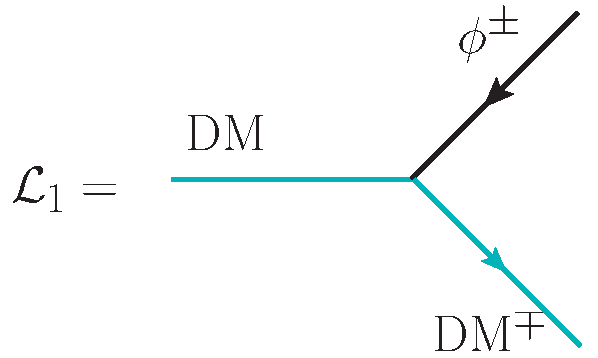
\includegraphics[height=1.4cm]{figures/dg1}}
}
\newcommand{\dgdos}{
\raisebox{-.5\height}{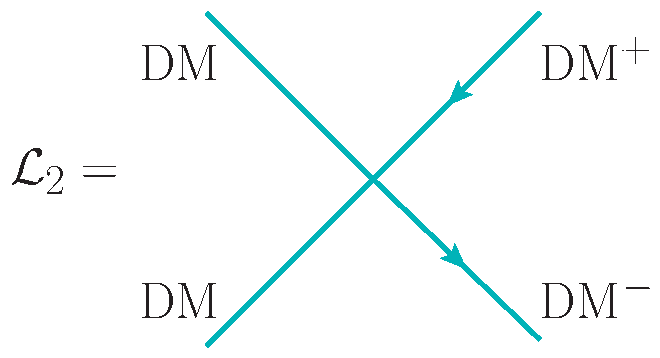
\includegraphics[height=1.4cm]{figures/dg2}}
}
\newcommand{\dgtres}{
\raisebox{-.5\height}{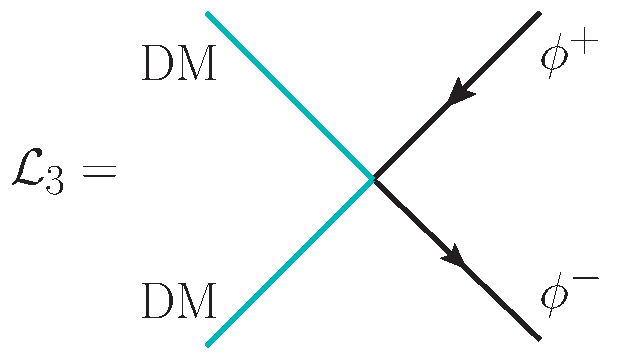
\includegraphics[height=1.4cm]{figures/dg3}}
}
\newcommand{\dgcuatro}{
\raisebox{-.5\height}{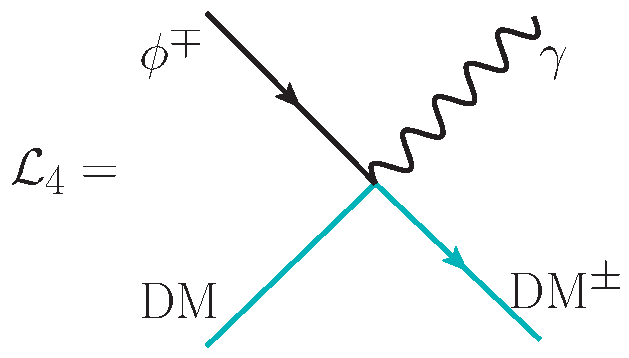
\includegraphics[height=1.4cm]{figures/dg4}}
%\newcommand{\Lfour}{${\cal L}_4$}%
}
%
\newcommand{\dgcinco}{
\raisebox{-.5\height}{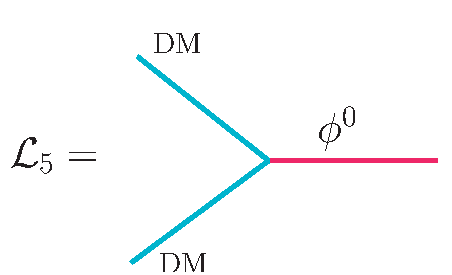
\includegraphics[height=1.6cm]{figures/dg5}}
}
%
\newcommand{\dgseis}{
\raisebox{-.5\height}{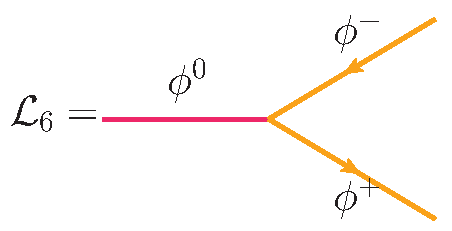
\includegraphics[height=1.3cm]{figures/dg6}}
}
%
\newcommand{\dgsiete}{
\raisebox{-.37\height}{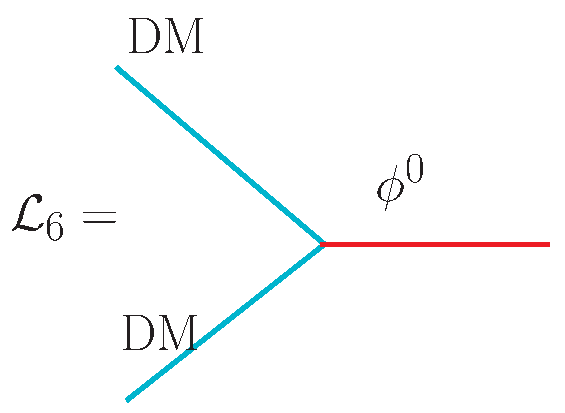
\includegraphics[height=1.7cm]{figures/dg7}}
}
%
\newcommand{\dgocho}{
\raisebox{-.5\height}{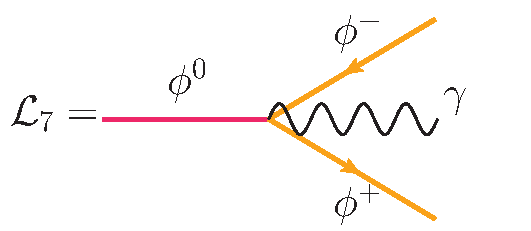
\includegraphics[height=1.7cm]{figures/dg8}}
}
%\newcommand{\Leleven}{{\small Tree-level coupling DM-$\gamma$}}%
\newcommand{\Leleven}{{\footnotesize   Violates (ii)}} %\hyperref[condition:ii]{(ii)}}}%
\newcommand{\Ltwelve}{{\footnotesize  Violates(iii)}} %\hyperref[condition:iii]{(iii) }}}%
%\newcommand{\Lfour}{
%\raisebox{-.5\height}{\includegraphics[height=1.7cm]{dg10}}
%}%
%%%%%%%%%%%%%%%%%%%%%%%%%%%%%%%%%%%%%%%%%%%%%%%%%%%%%%%%%%%%%%%%%%%%%%%%%%%%%%%%%%%%%%%%%%%%%%%%%%%%%%




%%%%%%%%%%%%%%%%%%%%%%%%%%%%%%%%%%%%%%%%%%%%%%%%%%%%%%%%%%%%%%%%%%%%%%%%%%%%%%%
%
%
%%%%%%%%%%%%%%%%%%%%%%%%%%%%%%%%%%%%%%%%%%%%%%%%%%%%
%% UNIVERSITY INFO 
%%%%%%%%%%%%%%%%%%%%%%%%%%%%%%%%%%%%%%%%%%%%%%%%%%%%
%
% University Name
%
	\UniversityName{Universidad de Antioquia}
%
% School Name
%
	\SchoolName{Instituto de Física}
%
% Department Name
%
	\DepartmentName{Facultad de Ciencias Exactas y Naturales \\
						{\large{Grupo de Fenomenolog\'ia de Interacciones Fundamentales (GFIF)}} }
%
% Location
%
	\UniversityLocation{Medellín}
%
%
%%%%%%%%%%%%%%%%%%%%%%%%%%%%%%%%%%%%%%%%%%%%%%%%%%%%
%% THESIS INFO 
%%%%%%%%%%%%%%%%%%%%%%%%%%%%%%%%%%%%%%%%%%%%%%%%%%%%
%
%% -------------------------------------------------------------------
% Thesis Type
%
	\ThesisType{\\PhD Thesis}
%
%% -------------------------------------------------------------------
% Thesis Title 
%
% To force line breaks in title, use "\\".
% If different line break locations are to be used for the cover page and the inner title page (page 3) 
% repeat the cover page title as an optional argument of the \title macro, including line breaks.
%
% Examples:
% 1. Automatic title line breaks in cover page and inner title page: 
%	    \title{This is my title}
% 2. Title breaking after ''my'' in both cover page and inner title page:
%	    \title{This is my \\ title}
% 3. Title breaking after ''my'' in cover page, and after ''is'' in inner title page:
%	    \title[This is my \\ title]{This is \\ my title}
%
	\title{ {\bf{\Large{\\Phenomenology of the singlet-doublet fermion scotogenic model }}} }
%%
%
%% -------------------------------------------------------------------
%% Thesis subtitle (optional)
%
% If no subtitle is required, set argument to blank, or comment-out the \subtitle macro.
%
% Example:
%%	\subtitle{This is my subtitle}
	\subtitle{}
%
%% -------------------------------------------------------------------
%
%% Author name
%
% For more than one authors, separate with ",".
% Example:
%	\authorName{Albert Einstein, George W. Bush} 
	\authorName{Andrés Felipe Rivera Romero} 
%
%% -------------------------------------------------------------------
%
%% Supervisor's name
% 
	\supervisor{Dr. Diego Alejandro Restrepo Q.\,,  }
	\cosupervisor{Dr. Oscar Alberto Zapata N.  }
%
%% -------------------------------------------------------------------
%% Supervisor's title
%
	\supervisorTitle{}
%
%
%% -------------------------------------------------------------------
%% Place and date of publication
%
	\thesisPlaceDate{Medellín, 2017}
%
%% -------------------------------------------------------------------
%% Place and date in acknowledgements (if applicable).
%
	\ackPlaceDate{Medellín, 2017}
%
%% -------------------------------------------------------------------
%% Approval information
%
	\examinationDate{ Date:}
	\approvalStatement{Approved by \hspace{2.0 cm}}
%
%% -------------------------------------------------------------------
%% Copyright Year
%
	\copyrightYear{2019}
%
%% -------------------------------------------------------------------
%% Name of first examiner
%
%	\firstExaminer{Professor A}
	\firstExaminer{\hspace{5.0 cm}}
%
%% -------------------------------------------------------------------
%% Title of first examiner
%
	\firstExaminerTitle{}
%
%% -------------------------------------------------------------------
%% Name of second examiner
%
	\secondExaminer{\hspace{5.0 cm}}
%
%% -------------------------------------------------------------------
%% Title of second examiner
%
	\secondExaminerTitle{}
%%
%%
%%%%%%%%%%%%%%%%%%%%%%%%%%%%%%%%%%%%%%%%%%%%%%%%%%%%%%%%%%%%%%%%%%%%%%
%% THESIS COLORS: 
%%%%%%%%%%%%%%%%%%%%%%%%%%%%%%%%%%%%%%%%%%%%%%%%%%%%%%%%%%%%%%%%%%%%%%
%%
%% Color for cover and chapters
	\chaptercolor{brown!75!magenta}
%%
%% Color for appendices
	\appendixcolor{brown!80!magenta}
%%
%% hyperlink color (ignored if the "hyperref" option is omitted)
    	\hyperlinkcolor{red!55!brown}
%%
%% Thesis title foreground color in cover page (ignored if the "plain" option is used)
    	\titlecolor{white}
%%
%% Thesis title background color in cover page (ignored if the "plain" option is used)
    	\titlebackgroundcolor{brown!85!magenta}  
%%
%%
%%%%%%%%%%%%%%%%%%%%%%%%%%%%%%%%%%%%%%%%%%%%%%%%%%%%%%%%%%%%%%%%%%%%%%
%% COVER PAGE IMAGE: 
%%%%%%%%%%%%%%%%%%%%%%%%%%%%%%%%%%%%%%%%%%%%%%%%%%%%%%%%%%%%%%%%%%%%%%
%%
%% Cover page image (optional)
%% If no cover page image is required, set argument to blank, or comment-out the \coverpageimage macro.
%%
%% Syntax:
%%          \coverpageimage{scale factor}{path to cover page image}
%%      or
%%          \coverpageimage[tikz]{scale factor}{TikZ commands}
%%          (commands may include \usetikzlibrary statements, etc.)
%%      
%% Examples:
%%      - Use the image in "figures/rdf.png" scaled by 0.8 (=80%):
%%          \coverpageimage{0.8}{figures/rdf.png}
%%      - Use a TikZ drawing scaled by 0.5 (=50%):
%%          \coverpageimage[tikz]{0.5}{
%%              \draw[thick, magenta] \foreach \x in {18,90,...,306} {
%%                  (\x:4) node{} -- (\x+72:4)
%%                  (\x:4) -- (\x:3) node{}
%%                  (\x:3) -- (\x+15:2) node{}
%%                  (\x:3) -- (\x-15:2) node{}
%%                  (\x+15:2) -- (\x+144-15:2)
%%                  (\x-15:2) -- (\x+144+15:2)
%%              };
%%          }
%%
     \coverpageimage{0.4}{figures/neutrino_mass_diagram}
     %\coverpageimage{0.3}{figures/bullet2}  
     \vspace{2.0 cm}
%%
%%
%%%%%%%%%%%%%%%%%%%%%%%%%%%%%%%%%%%%%%%%%%%%%%%%%%%%%%%%%%%%%%%%%%%%%%
%% MISCELLANEOUS SETTINGS: 
%%%%%%%%%%%%%%%%%%%%%%%%%%%%%%%%%%%%%%%%%%%%%%%%%%%%%%%%%%%%%%%%%%%%%%
%%
% Path to University Logo (all supported formats are allowed)
	%\UniversityLogoPath{logo/teikal_logo.eps}
	\UniversityLogoPath{figures/logo-udea}
%
% Path to University Logo (grayscale version to be used with the `printer' option)
	\UniversityBWLogoPath{figures/logo-udea.eps}
%
% Scalefactor for University logos (1 for 100%)
	\LogoScaleFactor{1.1}
% Draft Indication (watermark text to be used with the `watermark' option)
	\draftIndication{}%poner algo debajo de superviso en la primera hoja
%
% Frontispiece settings (ignored if the `frontispiece' option is omitted)
%	Syntax: \setFrontispiece[scale factor]{path to frontispiece image}{frontispiece image legend}
	\setFrontispiece[0.3]{figures/logo-udea}{Universidad de Antioquia} %figura detras de la primera página ---> GUITARRA
%
%%%%%%%%%%%%%%%%%%%%%%%%%%%%%%%%%%%%%%%%%%%%%%%%%%%%%%%%%%%%%%%%%%%%%%
%
% add custom hyphenation rules here
%\hyphenation{} 
%
%%%%
%
%
%%%%
\begin{document}

\maketitle

\beginfrontmatter
	
% Abstract (content in `abstract.tex')
	\begin{abstract}

In this thesis, we extend the singlet-doublet fermion dark matter model (SDFDM) with
additional $Z_2$--odd real  singlet scalars fields and we show that neutrino masses and mixings
can be generated at one-loop level.  We discuss the salient 
features arising from the combination of the two resulting
simplified dark matter models. 
%
Also, we examine the sensitivities of dark matter searches in the SDFDM scenario using \textit{Fermi}-LAT, CTA, IceCube/DeepCore, LUX, PICO and LHC with an emphasis on exploring the regions of the parameter space that can account for the excess of gamma rays from the Galactic Center (GCE).
 We find that DM particles present in this model with masses close to $\sim 99$ GeV and $\sim (173-190)$ GeV annihilating predominantly into the $W^+W^-$ channel and $t\bar{t}$ channel respectively, provide an acceptable fit to the GCE while being consistent with different current experimental bounds. We also find that much of the obtained parameter space can be ruled out by future direct search experiments such as LZ and XENON-1T.
Interestingly, we show that the most recent data by LUX is starting to probe the best fit region in the SDFDM model.
%
Moreover, we report a master equation for the velocity averaged annihilation cross section $\langle\sigma v\rangle$ of DM self-annihilation into two photons in a general model when the DM is its own antiparticle and whose stability is guaranteed by the $Z_2$ symmetry.
This master equation is general and leads to the same results found in the literature for popular dark matter candidates.

   \begin{keywords}
    	Dark matter, neutrino masses, scotogenic models, galactic center excess of gamma-rays
   \end{keywords}

\end{abstract}

% Dedication
	\thesisDedication{To my family and friends.
	\\Especially to Juliana for all your support.}
% Acknowledgements (content in `acknowledgements.tex')
	%%%%%%%%%%%%%%%%%%%%%%%%%%%%%%%%%%%%%%%%%%%%%%%%%%%%%%%%%%%%%%%%%%
%%
%% use the starred version of the "acknowledgements" environment
%% to omit signatures from this section, e.g.:
%% \begin{acknowledgements*} ... \end{acknowledgements*}
%% 
%%%%%%%%%%%%%%%%%%%%%%%%%%%%%%%%%%%%%%%%%%%%%%%%%%%%%%%%%%%%%%%%%
\begin{acknowledgements}

I would like to thanks all the people that in some way have helped me with the elaboration of this thesis.

First, I would like to thanks to my family. They are all that I have! My mom had always seen me as a superstar, my nephews always spoiling my homework but in a good way, my grandma always thinking that I am a mathematician, my brother and sister breaking their heads thinking why I spend a lot of time doing these strange things and \textit{Julianita} that has  been the way and my inspiration since she appeared on my way. All of them had encouraged me to follows this way without stopping in the difficult moments that always are there no matter where you are.

I would like to thanks to my advisors, the professor Oscar Zapata N. and especially to the professor Diego Alejandro Restrepo Q. for all the help, support, and amiability. He has been an excellent advisor. Sometimes he has shown me the way in those dark days of the academy work, discovering when I have been lost and pulling me when I have needed. 

Although it is difficult to list them, I would like to thanks to all my friends.  They always have been there with a good hand extended for me without taking care of my bad mood. Especially, I would like to thanks to the GFIF group. They have welcomed me and I have learned something from all of them.

Finally, I would like to thanks to COLCIENCIAS (Doctorado Nacional-6172) and the Institute of Physics at Universidad de Antioquia, the crazy place where I have spent a lot of time with the propose of complete this puzzle.

\end{acknowledgements}
% Table of Contents
	\tableofcontents
% List of Figures
	%\listoffigures
% List of Illustrations
	%\listofillustrations
% List of Tables
	%\listoftables
% Preface (content in `preface.tex') 
	%\begin{preface}
	Preface goes here ...  
\end{preface}
	
\beginmainmatter

%%%%%%%%%%%%%%%%%%%%%%%%%%%%%%%%%%%%%%%%%%%%%%%%%%%%%
%% INCLUDE YOUR CHAPTERS/SECTIONS HERE
%%
% Introduction
	\chapter{Physical problems addressed in this thesis} 
%
\InitialCharacter{T}he physical problems addressed in this thesis are introduced in this chapter. 
First, the dark matter (DM) observed in the Universe and the features that support its presence are explained. 
Also, the gamma-ray excess found in the galactic center of the Milky Way Galaxy is discussed in the context of the possible observation of DM annihilation. 
At the end, the chapter is focused in the neutrino masses and the possible relation between the DM and neutrino physics at one-loop level.  










\section{The dark matter in the Universe}
\label{sec:intro-dark-matter}
%
It is well established that the DM makes up about $26\%$ of the energy density of the Universe. It is about six times more abundant than ordinary matter~\cite{Ade:2015xua}.
However, its fundamental nature remains mysterious.
There is not known particle with the properties needed to constitute the DM, whose identity begs for new physics beyond the standard model (SM).
Unveiling which particle accounts for the majority of the matter in the Universe is a key open question at the interface of particle physics and cosmology.

Promising candidates for DM particles are weakly interacting massive particles (WIMPs).
These are generally assumed to be at equilibrium in the early Universe, but then freeze-out due to the rapid expansion of the Universe.
If the WIMP masses are in the GeV to TeV range, and the annihilation cross sections are of order the weak interaction scale, the relic DM density measured by experiments today arises naturally~\cite{Kolb:1990vq}.
% * <restrepo@udea.edu.co> 2016-09-21T12:20:31.236Z:
% 
% Esto ya no es del todo cierto. En esa época se referían a la mediación 
% con el Z que ya esta descartada.  Ver las slides de la charla de Oscar en Ibague, slide 16: 
% https://goo.gl/1s9QH8
% 
% ^. --> Falta (Andrés)
In general, there are some experimental facts that support the DM idea and therefore the structure formation in the Universe~\cite{Kolb:1990vq}. 
Some of them are shown in Fig.~\ref{fig:evidences} and they will be briefly discussed in the following. 
%
\begin{figure}[h]
\centering
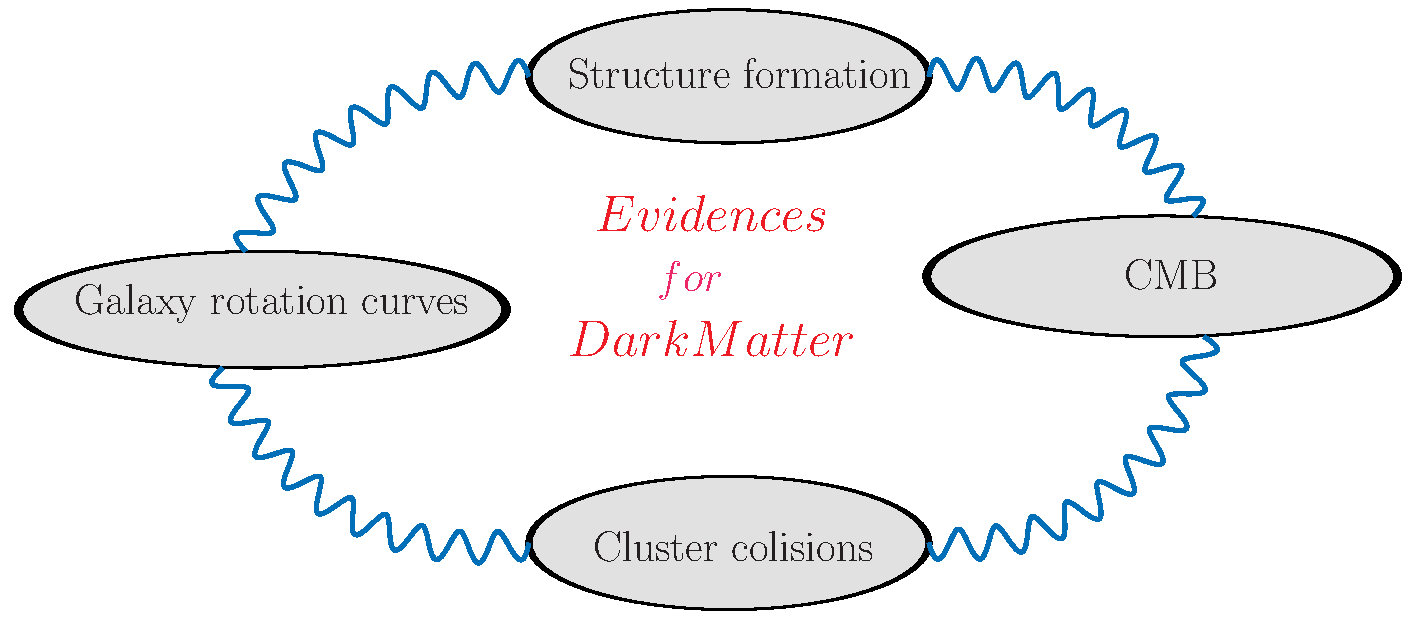
\includegraphics[width=10 cm, height=5.0 cm]{fig3.pdf}
\caption{Some of the most important evidences for Dark Matter.}
\label{fig:evidences}
\end{figure}










\begin{itemize}
\item[i.] \textbf{Galaxy rotation curves}

The rotation curve of a Galaxy (cluster) is the profile of the circular velocity
of the stars (galaxies) around the mass center of the system. 
It plays an important role because it is possible
to infer the mass distribution of the Galaxy (cluster)  after the analysis of this profile. 
Historically, the relation between the mass distribution and the rotation curve was first proposed by Fritz Zwicky in 1937.
He analyzed the velocity dispersion of the galaxies in the Coma cluster, assuming that the outer galaxies were in circular motion around its mass center.
He applied the virial theorem to the Coma cluster in order to estimate its mass and found that roughly 800 galaxies should  exhibit velocities of 80 km/h, however, the observed velocity dispersion was approximately 1000 km/h~\cite{1937ApJ-86-217Z}. 
The problem was known as the \textbf{Galaxy rotation problem} (for a complete historical discussion see the Ref.~\cite{Bertone:2016nfn}). 
%
\begin{figure}[h]
\begin{center}
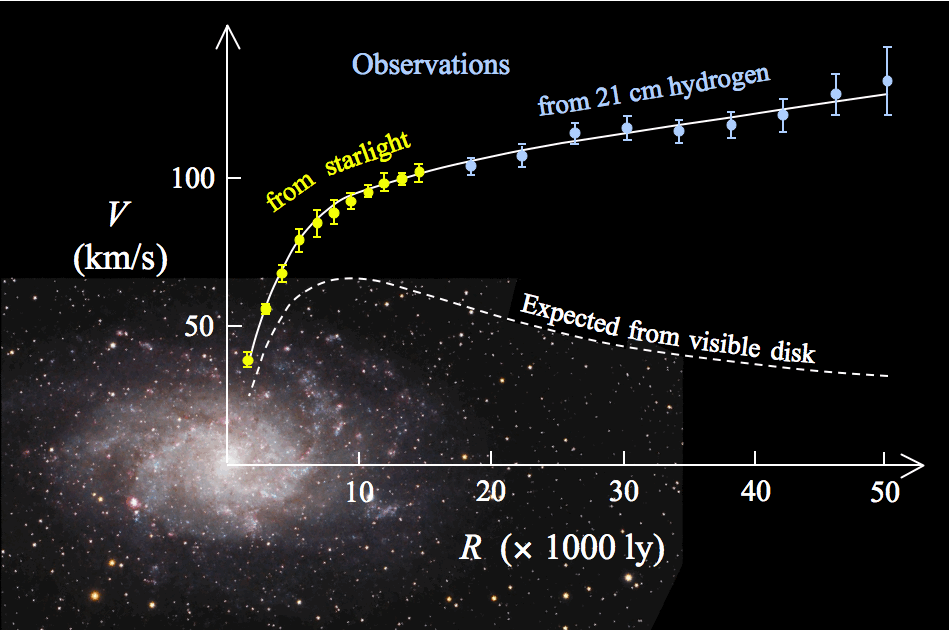
\includegraphics[scale=0.35]{M33_rotation_curve_HI}
\end{center}
\caption{Rotation curve of the typical spiral Galaxy M 33 (yellow and blue points with errorbars) and the predicted one from the distribution of the visible matter (white dashed line). The best fit model for rotation curve is represented by the continuous white line ~\cite{Corbelli:1999af} (Taken from Wikipedia - Public Domain).}
\label{fig:M33}
\end{figure}
%
The general idea under this problem is that when the Newton mechanics is used to explain the velocity distribution of the stars and visible gas in a Galaxy, the obtained profile (dashed white line in Fig.~\ref{fig:M33}) does not match with the observed behavior that is measured with some astrophysical techniques such as mass-to-light ratio~\footnote{The mass-to-light ratio ($\Upsilon$) is the relation between the total mass of a Galaxy and its luminosity. In astrophysics the reference value is the mass-to-light ratio of the sun, for that reason for big objects dominated by DM have a big mass-to-light ratio.} and the distribution of stars in the spiral galaxies.  
This problem is solved if the existence of dark hidden mass is supposed (dark, because it does not have electromagnetic interactions). Dark hidden mass is present in the Galaxy with a special distribution which governs its gravitational behavior, giving the characteristical name of \textit{dark matter} (DM).










\item[ii.] \textbf{The cosmic microwave background (CMB) }

\begin{figure}[h]
\begin{center}
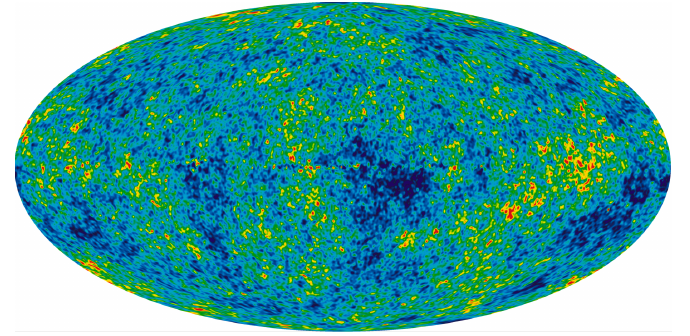
\includegraphics[scale=0.6]{CMB}
\end{center}
\caption{Nine Year Microwave Sky The detailed, all-sky picture of the infant Universe created from nine years of WMAP data. The image reveals $13.77$ billion-year-old temperature fluctuations (shown as color differences) that correspond to the seeds that grew to become the galaxies. The signal from our Galaxy was subtracted using the multi-frequency data. This image shows a temperature range of $\pm 200$ microKelvin. Credit: NASA / WMAP Science Team WMAP $\# 121238$ Image Caption $9$ year WMAP image of background cosmic radiation ($2012$).  (Taken from Wikipedia - Public Domain).}
\label{fig:CMB}
\end{figure}

The cosmic microwave background (CMB) is the oldest snapshot of the Universe that we have.
It is the thermal radiation when the Universe was approximate  $380.000$ years old after the big bang ($z\approx 1100, T\approx 3000$ K).
This radiation was generated in a time in the thermal history of the Universe called recombination or ``time of the last scattering'', which was the time when the electrons and protons formed bound states and created the neutral hydrogen in the Universe. Consequently, it was the time when the Universe began to be transparent to the photons because the atoms could not longer absorb the thermal radiation (photon decoupling). From that moment,  photons have been freely propagating.

The CMB was accidentally discovered in 1964 by the American radio astronomers Arno Penzias and Robert Wilson. For that achievement, they were awarded the Nobel Prize in 1978. This discovery was considered a big test of the big bang theory and the cosmological lambda cold dark matter model (Lambda-CDM or $\Lambda$-CDM).

In general, the CMB map shown in Fig.~\ref{fig:CMB} has a thermal black body spectrum at a temperature of $2.72548 \pm 0.00057$ K with a spectral radiance of 160.23 GHz, i.e. in the microwave range of frequencies. Even more, this spectrum  shows tiny temperature fluctuations that correspond to regions of slightly different densities that were the seeds of all the structures as the galaxies that are present in the Universe. 
%
Theoretically, those temperature fluctuations are generally expanded in the basis of spherical harmonics ($Y_{lm}$) as~\cite{Dodelson:1282338, Kolb:1990vq}
%
\begin{align}
\dfrac{\Delta T}{T}=\sum_{l,m} a_{l,m} Y_{lm}(\theta,\phi) \,,
\end{align}
%
where $\theta$ and $\phi$ are the spherical angles on the sky. Using this expansion, it follows that the two-point function of the coefficients $a_{lm}$:
%
\begin{align}
\langle a_{lm} a^*_{l^{'}m^{'}} \rangle = \dfrac{2\pi \delta_{ll^{'}}\delta_{mm^{'}}}{l(l+1)} \mathcal{D}_l \,,
\end{align}
%
determines the power spectrum of temperature $\mathcal{D}_l$ shown in Fig.~\ref{fig:T-spectrum}.
%
\begin{figure}[h]
\begin{center}
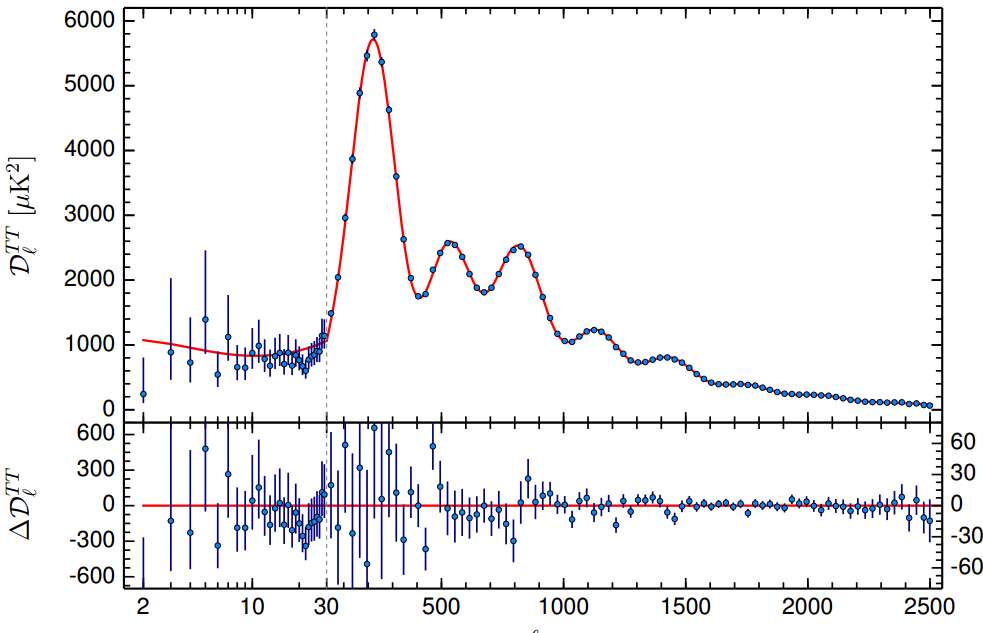
\includegraphics[scale=0.42]{spectrum}
\end{center}
\caption{Planck 2015 temperature power spectrum~\cite{Ade:2015xua}. For multipoles $l \geq 30$ is show the maximum likelihood frequency-averaged temperature spectrum. The best-fit, i.e. the $\Lambda$CDM theoretical spectrum is fitted in the upper panel. Residuals with respect to this model are shown in the lower panel. The error bars show $\pm \sigma$ uncertainties.}
\label{fig:T-spectrum}
\end{figure}

A careful analysis of the spectrum in Fig.~\ref{fig:T-spectrum} shows some special features associated with the primordial (secondary) anisotropies that occurred before (after) the photon decoupling, which are associated with the interactions of the background radiation with the hot gas and the gravitational potentials. Those anisotropies are principally determined by two effects that can be clearly seen in Fig.~\ref{fig:CMB} and Fig.~\ref{fig:T-spectrum}. Briefly, those are:
%
\begin{itemize}
\item[\textbullet ] The acoustic oscillation: In the primordial plasma there was a competition between the photons and baryons. The former tend to erase all the anisotropies and the later moving at a speed much slower than light tend to collapse to form overdensities. It is in this way that  the peaks of the CMB spectrum correspond to resonances in which the photons have decoupled from the plasma with a particular mode. 
Roughly speaking, the angular scale of the first peak in Fig.~\ref{fig:T-spectrum} with $l\approx 200$ ($\approx 1^o$ in galactic coordinates) determines the curvature of the Universe. For instance, the latest Planck data  combined with gravitational lensing and baryon acoustic oscillation (BAO)~\cite{Ade:2015xua} indicate that $\Omega_k = 0.000 \pm 0.005$ to $95\%$ confidence level. This means that the Universe is spatially flat at high precision.  
The ratio between the second and the first peak determines the baryon density. For instance, $\Omega_bh^2= 0.02230 \pm 0.00014$~\cite{Ade:2015xua}.
Finally, the third peak in combination with the first and the second peak can be used to obtain information about the dark matter density in the Universe, it is $\Omega_{\text{DM}}=(0.1197\pm 0.0022)$~\cite{Ade:2015xua}.

\item[\textbullet ] The diffusion damping: It is a physical process which reduced density inequalities (anisotropies) in the early Universe making the CMB more uniform. It happened when the photons traveled from the hot regions to the cold ones. It is important when the Boltzmann equation is computed for the CMB, which is not the scope of this work. 

\end{itemize}












\item[iii.] \textbf{Cluster collisions}

In $2006$ a group of astronomers published other direct empirical proof of the existence of the DM~\cite{Clowe:2006eq}. They studied the merging of two clusters of galaxies 1E 0657-558 ($z=0.296$) collectively known as the bullet cluster which collision is estimated that happened $\sim 100$ Mys ago and approximately in the plane determined by the velocities of the galaxies (see Fig.~\ref{fig:bullet}). 
%
In general, they found that there are two concentrations of galaxies separated by $\sim 0.72$ Mpc. The right one is moving away at $\sim 4700$ km s$^{-1}$ and it is creating a bow shock that gives its famous name of bullet cluster. 
%
\begin{figure}[h]
\centering
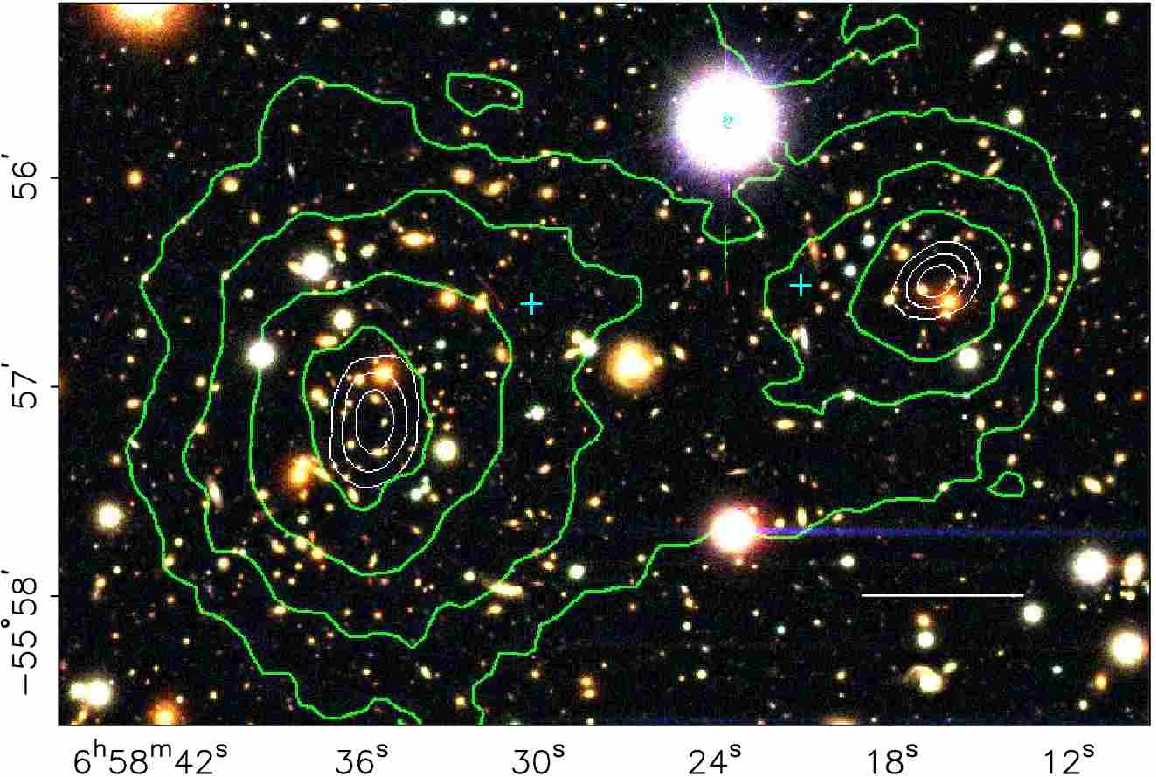
\includegraphics[scale=0.4]{bullet1}
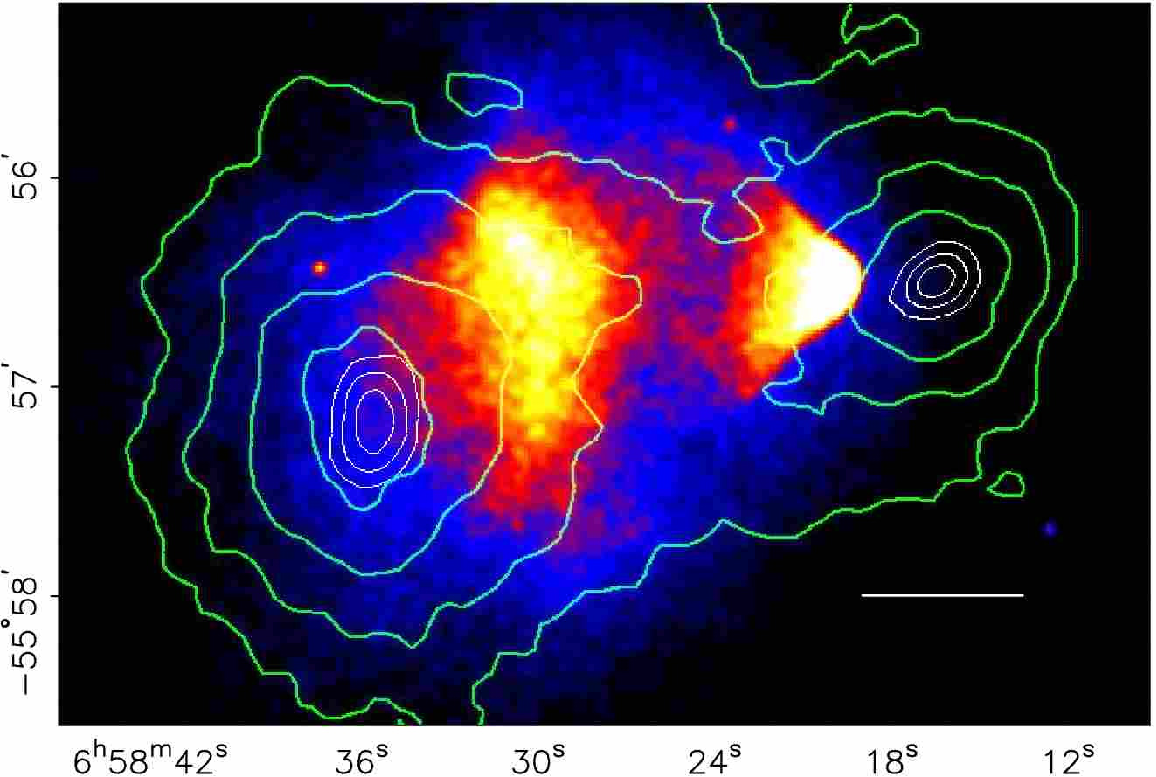
\includegraphics[scale=0.4]{bullet2}
\caption{The bullet cluster. The green contours are the reconstruction with gravitational lensing which is proportional to the mass of the system. The white bar represents a distance of $200$ kpc at the location of the cluster. The colored map on the right shows the same image seen in X-ray for the merging cluster. It was taken with the Chandra satellite after $500$ seconds of exposure. Taken from~\cite{Clowe:2006eq}.}
\label{fig:bullet}
\end{figure}
%

This observation is basically the discovery of one system in which the baryonic matter was separated from the mass center of each cluster involved in the collision. It was inferred as follows.
%
On the one hand, using gravitational lensing, the astronomers were able to reconstruct the contours of the mass projected for the system. They are represented by the green contours in Fig.~\ref{fig:bullet}. 
Basically, the gravitational lensing technique measures the distortion of the images caused by the gravitational deflection of light by the mass of the clusters and create a profile of the mass distribution inside the clusters itself. 
%
On the other hand, using the Chandra observation of X-rays they were able to see the X-rays emitted by the baryonic plasma of the system. The centers of the plasma are shown with the plus signs in the left panel of Fig.~\ref{fig:bullet}. Yellow and red parts of the image represent the baryonic plasma which emits the X-rays. Clearly, this hot plasma does not trace the mass distribution found with the gravitational lensing reconstruction. 

As a conclusion, during the merger, the galaxies behave to be almost collisionless and the hot plasma decouples of mass that is inferred by gravitational lensing. 
It can be understood if we think in two clouds of particles that are colliding. Almost all the particles pass through each other, i.e. they are collisionless and only the particles that represent the baryonic mass of the system collides.
According to this interpretation, the principal component of the mass of the system does not interact, it is dark (not baryonic) and correspond to the green contours shown in Fig.~\ref{fig:bullet}. 
%
Note that this observation is in favor of the DM interpretation as a particle. Even more, an alternative explanation using theories of Modified Newtonian Dynamics of the gravity  (MOND) does not predict an offset between mass and light and could fail to explain this observation of the bullet cluster~\cite{Angus:2006qy}.

\end{itemize}








%CONECTION
After this brief discussion of some of the facts that support the dark matter idea, it is important to describe briefly how to looking for  those  particles. 










\section{How to search for dark matter?}
\begin{itemize}

\item \textbf{Direct detection:}

The idea of direct detection of DM is based on the fact that DM particle (WIMP) is capable of collide with nucleons.
%For that reason, some experiments have been built with the purpose of collecting the signature when the DM collides with %nucleons.
%
In general, the cross section $\sigma$ for this interaction will depend on the naturalness of the DM. 
In particular, if the cross section depends of the spin of nucleons, it is called spin-dependent ($\sigma_{\text{SD}}$), otherwise,  spin-independent ($\sigma_{\text{SI}}$).
%
Until now, among the experiments for direct detection of DM, the most restrictive is the Large Underground Xenon experiment (LUX)~\footnote{\url{http://luxdarkmatter.org/}} ,
which is located 1,510 m underground at the Sanford Underground Laboratory in the Homestake Mine in Lead, South Dakota.
It is operated underground to reduce the noise signal caused by high-energy cosmic rays at the Earth's surface.
It is hoped that the interaction between DM and the liquid Xenon in the detector generates 175 nm ultraviolet photons and some electrons.
In this case, the photons will be detected by two arrays of 61 photomultiplier tubes at the top and bottom of the detector. 
The electrons generated by the particle interactions drift upwards through the xenon gas by an electric field and produce electroluminescence photons which are detected by the photomultiplier tubes. 
Those two signals commonly called S1 and S2 constitute the observable signal in the LUX experiment.
The last result of the LUX experiment for DM interaction spin-dependent and spin-independent are shown in Fig.~\ref{fig:LUX-SD-2016} and Fig.~\ref{fig:LUX-SI-2016} respectively. Not signal observed for DM is interpreted as an exclusion (region above lines).
%
\begin{figure}[h]
\begin{center}
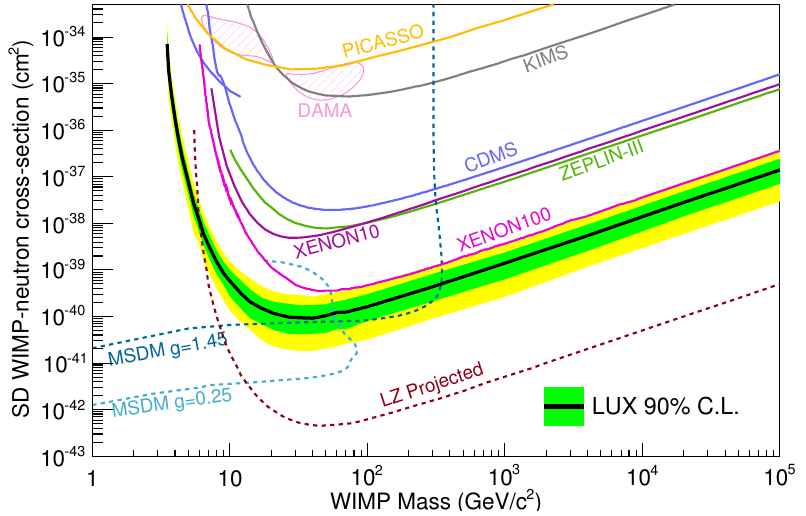
\includegraphics[scale=0.36]{LUX-SD-neutrons}
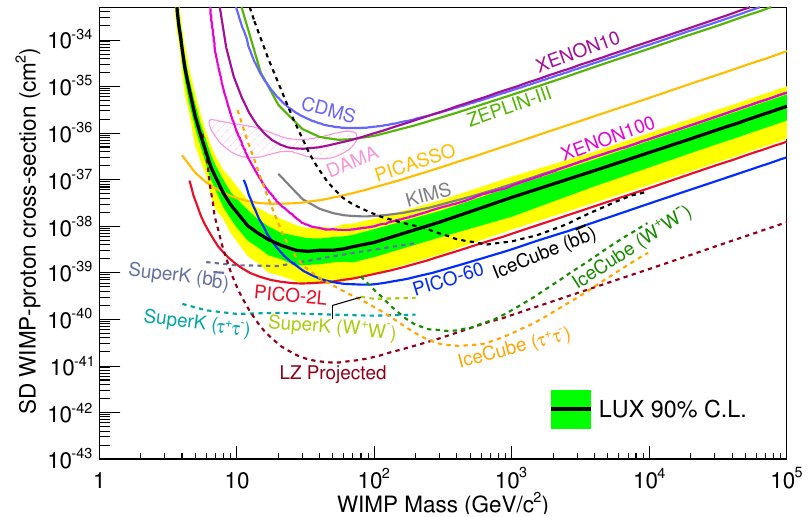
\includegraphics[scale=0.36]{LUX-SD-protons}
\end{center}
\caption{LUX upper limits on the WIMP-neutron (left) and -proton (right) elastic SD cross section at $90\%$ CL.
The Observed limit is shown in black with $\pm 1\sigma \, (\pm 2\sigma)$ band in green (yellow). Also, are shown the results from others experiments 
and the projected sensitivity for the LZ experiment. Taken from~\cite{Akerib:2016lao}. }
\label{fig:LUX-SD-2016}
\end{figure}
%
\begin{figure}[h]
\begin{center}
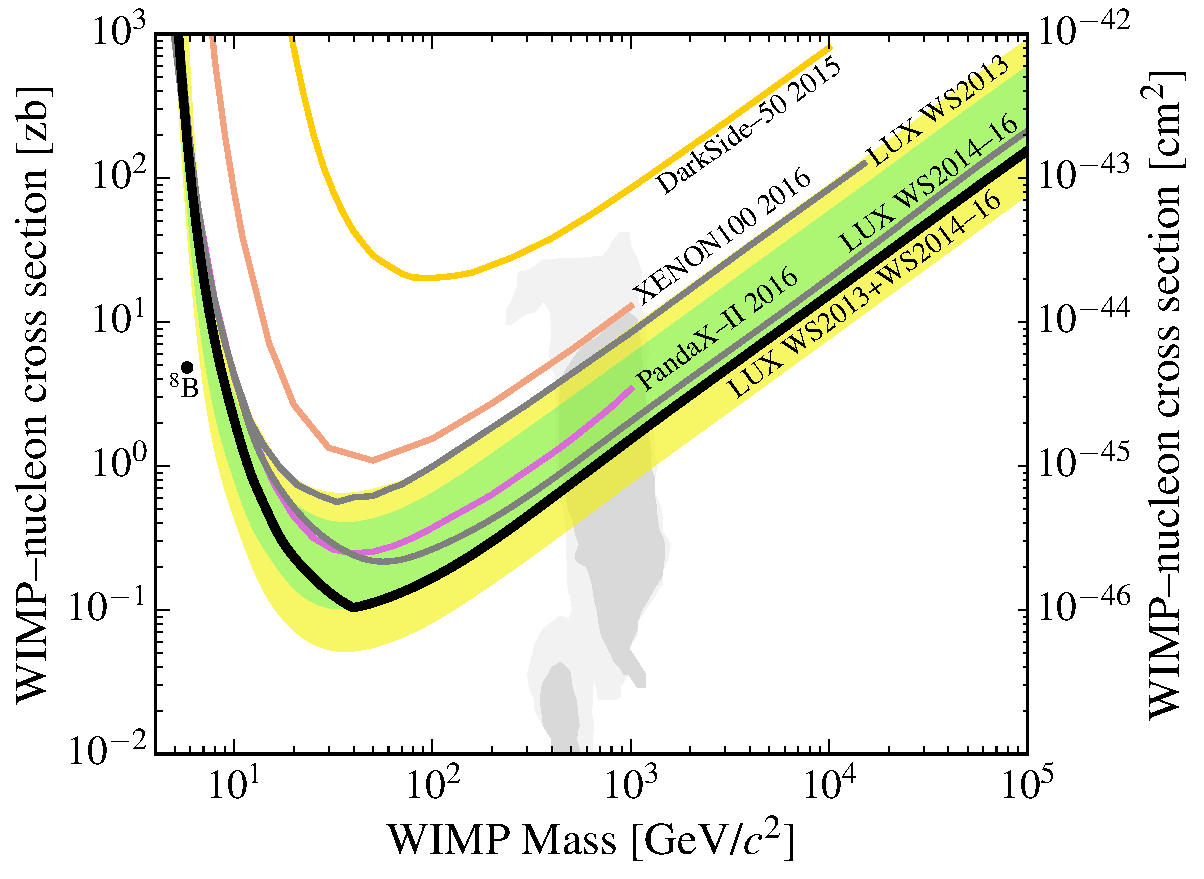
\includegraphics[width=10 cm,height=7 cm]{LUX-SI-2016}
\end{center}
\caption{LUX upper limits on the spin-independent elastic WIMP-nucleon
cross section at $90\%$ CL~\cite{Akerib:2016vxi}. }
\label{fig:LUX-SI-2016}
\end{figure}
%
The upper limits put strong constraints for all the DM theories based on the WIMP paradigm (Weakly Interacting Massive Particles). Specifically, all the region above the black line is excluded at $90\%$ CL.

\item \textbf{Indirect detection:}

Stable DM particles in the Universe could annihilate and produce a flux of gamma-rays, cosmic rays, neutrinos and anti-matter which can appear as an excess over the expected background, which is created by astrophysical features. In general, this flux can be written as
%
\begin{equation}
\underbrace{\frac{d\Phi}{d\Omega dE}}_{\text{Diff. Flux}} =  \frac{ \overbrace{\langle\sigma v \rangle}^{\text{Anni.\, Cross\, Section}}}{8\pi m_{\chi}^2} \times \underbrace{\frac{dN}{dE}}_{\text{Energy\, Spectrum}} \times \int_{\text{l.o.s}} ds \underbrace{\rho^2 (\overrightarrow{r}(s,\Omega))}_{\text{Dark\, Matter\, Distribution}},
\label{eq:flux}
\end{equation}
%
where $\Omega$ is the solid angle of the region of interest, $dN/dE$ is the energy spectrum (e.g. the number of particles produced per annihilation), $\sigma v$ is the annihilation cross section, and $\rho (\overrightarrow{r}(s,\Omega))$ is the DM density which should be integrated over the line of sight (l.o.s) from the observer to the source. This density is described by a specific profile, for instance, those shown in Table~\ref{table:DM-profiles}, where $\rho_{\odot}=0.3\, \text{GeV}/\text{cm}^3$ is the DM density at the sun, $r_s=20$~kpc is the scale radius of the halo and $R_{\odot}=8.5$~kpc is the distance from the sun to the center of the Galaxy~\cite{belanger2014micromegas}.
%
\begin{table}[h]
\centering
\begin{tabular}{|c|c|c|}\hline
Profile's name & Profile & \\\hline\hline
 & & \\
Zhao & $\rho(r) = \rho_{\odot} \left(\dfrac{R_{\odot}}{r}\right)^{\gamma} \left(\dfrac{r_s^{\alpha}+R_{\odot}^{\alpha}}{r_s^{\alpha}+r^{\alpha}}\right)^{\dfrac{\beta-\gamma}{\alpha}}$ & $\alpha=1$ \,, $\beta=3$ \,, $\gamma=1$ \\
 (in micrOMEGAS~\cite{belanger2014micromegas}) & &  \\\hline
 &  & \\
 Navarro-Frenk-White & $\rho(r) = \rho_{\odot}\, \frac{r_s}{r[1+ r/r_s]^2}$ & $\alpha=0.17$\\
 & & \\\hline
 &  & \\
Einasto profile & $\rho(r) = \rho_{\odot} \, exp \left[ -\frac{2}{\alpha} \left(\,  \left(\dfrac{r}{R_{\odot}}\right)^{\alpha}-1 \right) \right]$ &   $\alpha=0.17$ \\
 & & \\\hline
\end{tabular}
\caption{Mass density profiles for the dark matter in the Galaxy.}
\label{table:DM-profiles}
\end{table}

Several experiments for indirect detection of DM have been constructed. One of them is the \textit{Fermi} Large Area Telescope (\textit{Fermi}-LAT) which has a particle detector on board the Fermi gamma-ray space telescope spacecraft launched in 2008~\footnote{\url{http://fermi.gsfc.nasa.gov/}}. 
%
The searches of this experiment are focused in numerous exotic and beautiful phenomena, which can generate a lot of energy. For instance, Supermassive black holes, merging neutron stars, streams of hot gas moving close to the speed of light, etc. 
These are some of the marvels that generate gamma-ray radiation and the telescope is prepared to see it.
%
One of the searches has been concentrated in the dwarf spheroidal satellite galaxies (dSphs) of the Milky Way Galaxy, which are one of the most DM dominated objects known. 
In general, the \textit{Fermi}-LAT measures the flux of gamma-rays and reconstructs the signal as an interpretation of DM annihilation. 
Until now, the satellite has not seen a DM signal. 
However, it has presented upper limits on the thermal velocity averaged annihilation cross section $\langle \sigma v \rangle$ using some combined analysis~\cite{Ackermann:2015zua}. 
One of the principal results for DM self-annihilation are based on the photons created by the hadronization of the quarks, for instance, after the process $\text{DM DM} \to q\bar{q}$. 
The previous fact gives us a strong constraint in the $\langle \sigma v \rangle$ and will play an important roll in some of the analysis in this thesis.
 
%CONNECTION
Regarding indirect detection of dark matter, there is currently a puzzle related to the observation of an excess of gamma-ray with the \textit{Fermi}-LAT satellite that is one of the topics addressed in this thesis and for that reason will be briefly described in the next section.

\end{itemize}











%%%%%%%%%%%%%%%%%%%%%%%%%%%%%%%%%%%%%%%%%%%%%%%%%%%%%%%%%%%%%%%%%%%%%
\section{Dark matter interpretation of the galactic center excess}
\label{sec:intro-gce}
%
%TEXTO AMPLIADO DEL PAPER... MUCHOS PARRAFOS SON COPIADOS LITERALMENTE
WIMP particles appear effortlessly in many extensions of the SM that resolve outstanding theoretical and phenomenological problems which are not necessarily related to the DM puzzle.
 In some of these models, WIMPs can be produced in high energy colliders (collider DM searches), in elastic scatter with nucleons (direct DM searches) or in the annihilation and production of observable particles in astrophysical environments (indirect DM searches).
 High-energy photons in the gamma-ray ($\gamma$-ray) frequency constitute the most notable search channel of the latter category because they can travel almost unperturbed from their sources to the detectors.
 The Large Area Telescope on board the \textit{Fermi} satellite (\textit{Fermi}-LAT)~\cite{Fermi} is the most sensitive $\gamma$-ray detector in the range from 20 MeV to 300 GeV~\cite{Ackermann:2015zua}.

At the bottom of the gravitational well of the Milky Way Galaxy, the Galactic Center (GC) is expected to be the region displaying the brightest emission of DM annihilations in the $\gamma$-ray sky~\cite{Funk:review}.
However, there are multitude of non-thermal astrophysical sources in that region that complicate the identification of a tentative DM signal~\cite{Funk:review}. Observations of the inner few degrees around the GC with the \textit{Fermi}-LAT have revealed an excess of $\gamma$-rays ~\cite{Goodenough2009gk,Vitale:2009hr,Hooper:2010mq,hooper,AbazajianKaplinghat2012,AbazajianKaplinghat2013,GordonMacias2013}. 
The spectrum of the Galactic Center excess (GCE) peaks at about 1-3 GeV and its spatial morphology is spherically symmetric varying with radius $r$ around the GC as $r^{-2\gamma}$ with  $\gamma\sim 1.2$ which is clearly compatible with the DM density profile. 
This emission has been found to extend out in Galactic latitude ($b$) up to about $|b|\lesssim 20^\circ$ ~\cite{hooperslatyer2013,Daylan:2014,CaloreCholisWeniger2015,TheFermi-LAT:2015kwa} and its presence appears  to be robust with respect to systematic uncertainties~\cite{GordonMacias2013,MaciasGordon2014,Daylan:2014,Zho2015,CaloreCholisWeniger2015,PorterMurgia2015,TheFermi-LAT:2015kwa}.

Fig.~\ref{fig:GCE-less2} shows the GCE observed for $|b|<2^{\circ}$ and Galactic longitude $|l|<2^{\circ}$. 
This is the remaining excess after subtracting the Gamma Diffuse Emission of gamma rays (GDE) produced by cosmic rays that generate pions $\pi^0$ in collisions with the interstellar gas that latter decay and produce photons, by cosmic electrons which produce photons by bremsstrahlung emission and by photons accelerated by Inverse Compton scattering (ICS).
Fig.~\ref{fig:GCE-bigger2} shows the complete signal observed of the Galaxy for   $|b|>2^{\circ}$ and the remaining GCE after cleaning the map using the best GDE models. 

\begin{figure}[h]
\begin{center}
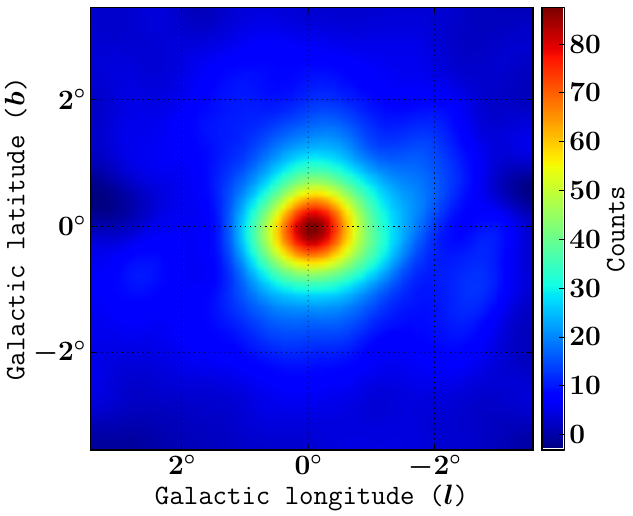
\includegraphics[scale=0.4]{latitude-less2}
\end{center}
\caption{Residual map or GCE signal for $|b,l|<2^{\circ}$. The counts were summed over the energy range 
$300$ MeV-$10$ GeV. The map spans a $7^{\circ}\times 7^{\circ}$ region of the sky centred in the Sgr A$^*$ position with a pixel size of $0.1^{\circ}\times 0.1^{\circ}$. Taken from~\cite{GordonMacias2013}.}
\label{fig:GCE-less2}
\end{figure}
%
\begin{figure}[h]
\begin{center}
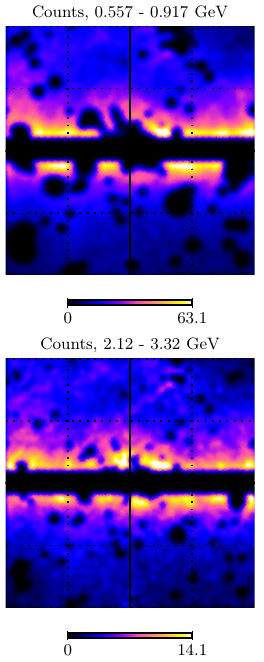
\includegraphics[scale=0.6]{latitude-bigger2a}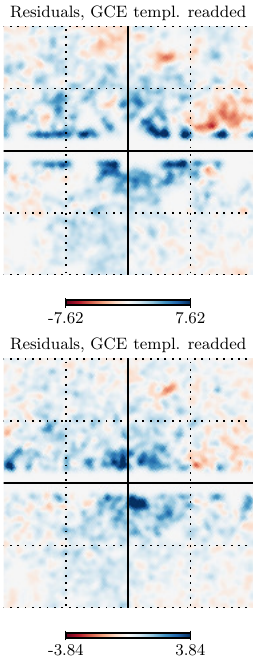
\includegraphics[scale=0.6]{latitude-bigger2b}
\end{center}
\caption{\textit{Left panels}: Counts map a various energies, with the disk cut $|b|>2^{\circ}$. \textit{Right panels}: Residual after sustracting the best Gamma Difuse emition model (GDE). Taken from~\cite{CaloreCholisWeniger2015}.}
\label{fig:GCE-bigger2}
\end{figure} 

There is an ongoing and intense debate as to what the origin of this signal is. A tentative explanation is an unresolved population of $\sim 1000$ millisecond pulsars (MSPs)~\cite{Abazajian:2010zy,AbazajianKaplinghat2012,Wharton2012,GordonMacias2013,GordonMacias2013erratum,Mirabal2013,MaciasGordon2014,YuanZhang2014,BrandtKocsis2015,Lacroix:2015wfx,O'Leary:2016osi} or young pulsars \cite{OLeary2015,O'Leary:2016osi}.
 Nevertheless, some studies~\cite{Hooper2013,CholisHooperLinden2015,PetrovicSerpicoZaharijas2015,Lee2015,BartelsKrishnamurthyWeniger2015,Linden2015} have pointed out about the difficulties of reconciling this hypothesis with the GCE extending out as far as $\sim 10^\circ$ from the GC. On the other hand, recent works claim that the GCE is not smooth~\cite{Lee:2015fea,Bartels:2015aea}, and if confirmed, this would lend support to the MSPs alternative.
 Another scenario put forward is a series of energetic cosmic-ray injections in the GC \cite{CarlsonProfumo,Petrovic2014}.
 However, if the injected particles are mainly protons, it has been shown~\cite{MacGorCroProf2015} that this scenario is incompatible with the spatial morphology of the GCE in the inner $\sim 2^\circ$ of the Galaxy.
 In case the burst events contain protons as well as leptons, Ref~\cite{Cholis2015} finds suitable models that appear fine-tuned.

Despite these astrophysical uncertainties, a DM interpretation of the GCE cannot be ruled out yet~\cite{Goodenough2009gk,Hooper:2010mq,hooper,AbazajianKaplinghat2012,AbazajianKaplinghat2013,GordonMacias2013,MaciasGordon2014,Abazajian2014,Daylan:2014,Lacroix:2015wfx}.
   In this context, the spatial morphology of the GCE can be accommodated with a Navarro-Frenk-White (NFW) profile with a mildly contracted cusp of $\gamma\sim 1.2$, the measured spectrum implies a WIMP mass in the GeV energy range and an interaction cross section that coincides with the thermal relic cross section. 

A recent study of the GCE~\cite{CaloreCholisWeniger2015} selected a target region ($|b|>2^\circ$) that excluded the core of the GC. Additionally, the systematic uncertainties in the Galactic diffuse emission were estimated in a manner that made the low and high energy tails of the spectrum more uncertain than in previous analyses~\cite{GordonMacias2013,MaciasGordon2014,Abazajian2014,Daylan:2014}, which focused on a smaller region containing the inner $\sim 2^\circ$ of the GC. Although it is possible that the greater degree of uncertainty in the tails found by~\cite{CaloreCholisWeniger2015} is due to an intricate overlap of the GCE with the Fermi Bubbles~\cite{suslatyerfinkbeiner2010,Fermi-LAT:AnnaFranckowiak}, it is interesting that this uncertainty also allows much more freedom for DM models fitting the GCE~\cite{Logan:2010nw,Buckley:2010ve,Zhu:2011dz,Marshall:2011mm,Boucenna:2011hy,Buckley:2011mm,Anchordoqui:2013pta,Buckley:2013sca,Hagiwara:2013qya,Okada:2013bna,Huang:2013apa,Modak:2013jya,Boehm:2014hva,Alves:2014yha,Berlin:2014tja,Agrawal:2014una,Izaguirre:2014vva,Cerdeno:2014cda,Ipek:2014gua,Boehm:2014bia,Ko:2014gha,Abdullah:2014lla,Ghosh:2014pwa,Martin:2014sxa,Basak:2014sza,Berlin:2014pya,Cline:2014dwa,Han:2014nba,Detmold:2014qqa,Wang:2014elb,Chang:2014lxa,Arina:2014yna,Cheung:2014lqa,McDermott:2014rqa,Huang:2014cla,Balazs:2014jla,Ko:2014loa,Okada:2014usa,Ghorbani:2014qpa,Banik:2014eda,Borah:2014ska,Cahill-Rowley:2014ora,Guo:2014gra,Freytsis:2014sua,Heikinheimo:2014xza,Arcadi:2014lta,Richard:2014vfa,Cao:2014efa,Bell:2014xta,Cerdeno:2015ega,Caron:2015wda,Bertoneetal,Freeseetal}.  


Significant effort has been made in exploring the properties of DM models that can explain the GCE while being consistent with other indirect, direct and collider constraints~\cite{Logan:2010nw,Buckley:2010ve,Zhu:2011dz,Marshall:2011mm,Boucenna:2011hy,Buckley:2011mm,Anchordoqui:2013pta,Buckley:2013sca,Hagiwara:2013qya,Okada:2013bna,Huang:2013apa,Modak:2013jya,Boehm:2014hva,Alves:2014yha,Berlin:2014tja,Agrawal:2014una,Izaguirre:2014vva,Cerdeno:2014cda,Ipek:2014gua,Boehm:2014bia,Ko:2014gha,Abdullah:2014lla,Ghosh:2014pwa,Martin:2014sxa,Basak:2014sza,Berlin:2014pya,Cline:2014dwa,Han:2014nba,Detmold:2014qqa,Wang:2014elb,Chang:2014lxa,Arina:2014yna,Cheung:2014lqa,McDermott:2014rqa,Huang:2014cla,Balazs:2014jla,Ko:2014loa,Okada:2014usa,Ghorbani:2014qpa,Banik:2014eda,Borah:2014ska,Cahill-Rowley:2014ora,Guo:2014gra,Freytsis:2014sua,Heikinheimo:2014xza,Arcadi:2014lta,Richard:2014vfa,Cao:2014efa,Bell:2014xta,Cerdeno:2015ega,Caron:2015wda,Bertoneetal,Freeseetal}.
 Of great interest are the properties of minimal supersymmetric extensions of the SM (MSSM)~\cite{Cheung:2014lqa,Cahill-Rowley:2014ora,Cao:2014efa,Cerdeno:2015ega,Caron:2015wda,Bertoneetal,Freeseetal} that can fit the GCE.
 When these extensions are studied in light of the GCE extracted from the region $|b|>2^\circ$ of the GC, the required neutralino annihilation rates to mainly the $W^+W^-$ and $\bar{t}t$ channels are found to comply with the LEP or LHC bounds on sfermion masses.
However, we do not restrict ourselves to supersymmetric models. Instead, we take the approach of studying a simplified DM model in which the DM candidate is a mixture, generated by the interaction with the Higgs boson, of a SM fermion singlet and the neutral components of an electroweak doublet vector-like fermion~\cite{ArkaniHamed:2005yv,Mahbubani:2005pt,D'Eramo:2007ga,Enberg:2007rp}. This model, also known as the singlet$-$doublet fermion DM (SDFDM) model, is one of the simplest UV realizations of the fermion Higgs portal ~\cite{Patt:2006fw} with the SM Higgs boson as the mediator between the visible and dark sectors. In fact, the dark sector of the SDFDM model (along with the stabilizing discrete symmetry) is part of the minimal setup expected when the SM is extended by new physics which is to some extent related to lepton and baryon number conservation~\cite{Arbelaez:2015ila,Arkani-Hamed:2015vfh}. While being free of many theoretical biases, this  model allows us to extract maximal phenomenological information from a framework that is a good representation of the WIMP paradigm \cite{ArkaniHamed:2005yv,Mahbubani:2005pt,D'Eramo:2007ga,Enberg:2007rp,Cohen:2011ec,Cheung:2013dua,Abe:2014gua,Calibbi:2015nha,Freitas:2015hsa,Abdallah:2015ter}.%\footnote{ If scalar singlets are added to its particle content, neutrino masses can also be radiatively generated in this generic class of models~\cite{Restrepo:2015ura}.}.     
Accordingly, the SDFDM model is set to become one of the models to be implemented in future searches for DM particles at the LHC \cite{Abdallah:2015ter} and a future 100 TeV hadron collider \cite{Gori:2014oua,Arkani-Hamed:2015vfh}.  

To understand how neutrino masses will be incorporated in a SDFDM model, it is important to explain briefly the relation between the dark matter and neutrino masses, more specifically, how to generated neutrino masses from a dark sector. This relation will be described in the next section.











%%%%%%%%%%%%%%%%%%%%%%%%%%%%%%%%%%%%%%%%%%%%%%%%%%%%%%%%%%%%%%%%%%%%%
\section{Relations between dark matter and the non-zero neutrino masses}

\subsection*{Neutrino physics in a nutshell}
\label{sec:intro-neutrino}
%
Although, neutrinos in the SM are massless, current neutrino oscillation data had established the non-zero value of neutrino masses, which is a clear indication of new physics beyond the SM. 
These neutrino data can be described within the framework of a $3\times 3$ mixing matrix $U$ between the flavor eigenstates $\nu_l=(\nu_e,\nu_{\mu},\nu_{\tau})$ and the mass eigenstates $\nu_i=(\nu_1,\nu_2,\nu_3)$, such that
%
\begin{align}
|\nu_l\rangle = \sum_i U_{li}^*|\nu_i\rangle \,.
\end{align}
%
In the case of Dirac neutrinos, the mixing matrix  $U$ depends on three mixing angles $\theta_{12}$, $\theta_{13}$, $\theta_{23}$ and one CP-violating phase $\delta$, while in the case of Majorana neutrinos there are two additional phases~\cite{Akhmedov:1999uz}. 
In general, it is convenient to use the parametrization that coincides with the quark mixing matrix given by
%
\begin{displaymath}
U=\left(\begin{array}{c c c}
c_{12}c_{13} & s_{12}c_{13}& s_{13}e^{-i\delta}\\
-s_{12}c_{23}-c_{12}s_{23}s_{13}e^{i\delta} & c_{12}c_{23}-s_{12}s_{23}s_{13}e^{i\delta} & s_{23}c_{13}\\
s_{12}s_{23}-c_{12}c_{23}s_{13}e^{i\delta} & -c_{12}s_{23}-s_{12}c_{23}s_{13}e^{i\delta} & c_{23}c_{13}
\end{array} \right)\,,
\end{displaymath}
%
where $c_{ij}=\cos \theta_{ij}$ and $s_{ij}=\sin \theta_{ij}$.

In the neutrino oscillation theory, the probability of the transformation of a flavor eigenstates neutrino $\nu_{a}$ into another one $\nu_{b}$ in a time $t$ is given by~\cite{Akhmedov:1999uz}
%
\begin{align}
P(\nu_a \to \nu_b; t)=|U_{bj}e^{-iE_j t}U_{aj}^*|^2\,,
\end{align}
%
where the energy $E_i$ and the momenta $p$ for the eigenstate of mass $m_i$ are related by
\begin{align}
E_i=\sqrt{p^2+m_i^2}\approx p+\dfrac{m_i^2}{2p}\,.
\end{align}
%
There are some important limit cases in which this probability is computed. For instance, when the neutrino mass squared differences $\Delta m_{ij}^2=m_i^2-m_j^2$ have a hierarchy
%
\begin{align}
|\Delta m_{21}^2| \ll |\Delta m_{31}^2| \simeq |\Delta m_{32}^2|
\Rightarrow
\left\{
\begin{array}{ll}
 m_1 \ll (\lesssim)\, m_2 \ll m_3 & \text{ Normal hierarchy NH } \\
 m_3 \ll m_1 \approx m_2 & \text{ Inverted  hierarchy IH }\,.
\end{array}
\right. 
\end{align}
%
These hierarchies are good motivated by the fact that the solar neutrino data indicates $\Delta m_{21}^2 =\Delta m_{\odot}^2 \sim 10^{-5}$ eV$^2$ for the solution of the solar neutrino problem through the matter neutrino oscillations ($\Delta m_{\odot}^2 \sim 10^{-10}$ eV$^2$ through the vacuum oscillations).  Whereas the explanation of the atmospheric neutrino oscillations experiments requires $\Delta m_{32}^2 =\Delta m_{\text{atm}}^2 \sim 10^{-3}$ eV$^2$ much larger than  $\Delta m_{\odot}^2$. For a complete list of neutrino oscillation parameters see Table~\ref{tab:neutrino-parameters}.

\begin{table}[h]\centering
   \begin{tabular}{lccc}
    \hline
    parameter & best fit $\pm$ $1\sigma$ &  2$\sigma$ range& 3$\sigma$ range
    \\
    \hline
    $\Delta m^2_{21}\: [10^{-5}\eVq]$
    & 7.60$^{+0.19}_{-0.18}$  & 7.26--7.99 & 7.11--8.18 \\[3mm] 
    %%
    $|\Delta m^2_{31}|\: [10^{-3}\eVq]$ (NH)
    &  2.48$^{+0.05}_{-0.07}$ &  2.35--2.59 &  2.30--2.65\\
    $|\Delta m^2_{31}|\: [10^{-3}\eVq]$ (IH)
    &  2.38$^{+0.05}_{-0.06}$ &  2.26--2.48 &  2.20--2.54 \\[3mm] 
    %%	
    $\sin^2\theta_{12} / 10^{-1}$
    & 3.23$\pm$0.16 & 2.92--3.57 & 2.78--3.75\\
    $\theta_{12}$ 
    & 34.6$\pm$1.0 & 32.7--36.7 & 31.8--37.8\\[3mm]  
    %%
    $\sin^2\theta_{23} / 10^{-1}$ (NH)
    &	5.67$^{+0.32}_{-1.28}$ 
    & 4.13--6.23 & 3.92 -- 6.43 \\
    $\theta_{23}$ %(NH)
    & 48.9$^{+1.9}_{-7.4}$ & 40.0--52.1 & 38.8--53.3 \\ 
    $\sin^2\theta_{23} / 10^{-1}$ (IH)
    & 5.73$^{+0.25}_{-0.43}$ & 4.32--6.21 & 4.03--6.40 \\
    $\theta_{23}$ %(IH)
    & 49.2$^{+1.5}_{-2.5}$ & 41.1--52.0 & 39.4--53.1\\[3mm]  
    %%	
    $\sin^2\theta_{13} / 10^{-2}$ (NH)
    & 2.34$\pm$0.20 & 1.95--2.74 & 1.77--2.94 \\
    $\theta_{13}$ %(NH)
    &	8.8$\pm$0.4 & 8.0--9.5 & 7.7--9.9\\
    $\sin^2\theta_{13} / 10^{-2}$ (IH)
    & 2.40$\pm$0.19 & 2.02--2.78 & 1.83--2.97 \\
     $\theta_{13}$ %(IH)
     & 8.9$\pm$0.4 & 8.2--9.6 & 7.8--9.9\\[3mm]
    %%	
   $\delta/\pi$ (NH)
   	& 1.34$^{+0.64}_{-0.38}$ & 0.0--2.0 & 0.0--2.0 \\
   $\delta/\pi$ (IH)	
   	& 1.48$^{+0.34}_{-0.32}$ & 0.0--0.14 \& 0.81-2.0 & 0.0--2.0 \\	
       \hline
     \end{tabular}
     \caption{ \label{tab:summary} Neutrino oscillation parameters
       summary taken from~\cite{Forero:2014bxa}. For $\Delta m^2_{31}$, $\sin^2\theta_{23}$, $\sin^2\theta_{13}$, 
       and $\delta$ the upper (lower) row corresponds to normal (inverted)
       neutrino mass hierarchy.}
\label{tab:neutrino-parameters}
\end{table}











\subsection*{How to generate neutrino masses from a dark sector?}
%
In this thesis, it is assumed that the neutrinos of the SM are Majorana particles.
In that case, their so small masses can be understood if there is a new physics beyond the SM as it will briefly describe in the present section. 
It have been shown that the lower operator which generates Majorana neutrino masses is the $d=5$ Weinberg operator~\cite{PhysRevLett.43.1566}
%
\begin{align}
\label{eq:weinberg-operator}
\mathcal{L}=\dfrac{1}{2}c_{\alpha\beta}^{d=5} \,\, \left(\overline{L_{\alpha}^c}\widetilde{H}^*\right) \left( \widetilde{H}^{\dagger}L_{\beta}\right) + \text{h.c.}  \,,
\end{align}
%
where $H=\left(H^+,H^0\right)^T$ is the Higgs doublet, $\widetilde{H}=i\sigma_2 H^*$,  $L_{\alpha}=\left(\nu_{\alpha L},e_{\alpha L}\right)^T$ are the left-handed lepton doublets of the SM with $\alpha$ the flavor number and $c_{\alpha\beta}^{d=5}\propto 1/\Lambda $ is a model dependent coefficient that characterize the scale of the new physics.  
All the models where the neutrinos are Majorana particles are reduced to this operator or a higher dimensional equivalent $(d > 5)$ when the new physics is integrated out~\cite{Bonnet:2012kz}.

At tree level, there are three ways to generate this operator. These are known as type-I, type-II and type-III see-saw mechanisms when the mediator is a singlet fermion $N$, a triplet scalar $\Delta$ or a triplet fermion $\Sigma$ respectively. These three cases are schematically shown in Fig.~\ref{fig:see-saw-tree-level}.
%
\begin{figure}[h]
\begin{center}
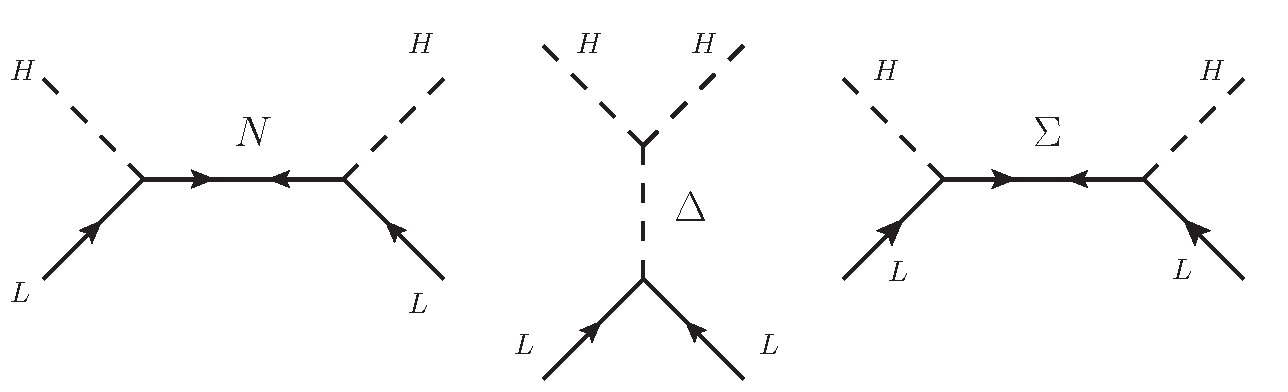
\includegraphics[scale=0.7]{fig4.pdf}
\end{center}
\caption{The three realizations of the see-saw mechanism at tree level.}
\label{fig:see-saw-tree-level}
\end{figure} 

From Eq.~\eqref{eq:weinberg-operator} we can see that the neutrino mass scale is roughly given by $m_{\nu_{\alpha}}\propto \langle H^0\rangle^2/\Lambda$,  where $\langle H^0\rangle$ is the vacuum expectation value of the SM Higgs boson. Notice that in order to have small neutrino masses the $\Lambda$ points to the scale of a grand unified theory (GUT).  
%Therefore, in these see-saw models the new physics scale will be impossible to test at the LHC.

On the other hand, at one-loop level, when the neutrino masses are generated radiatively, 
one additional suppression comes from the loop.
In this case, the new physics and consequently the dark sector could be at the electroweak scale (EW) and the mechanism could be tested with the current direct, indirect and colliders experiments.
%
\begin{figure}[h]
\begin{center}
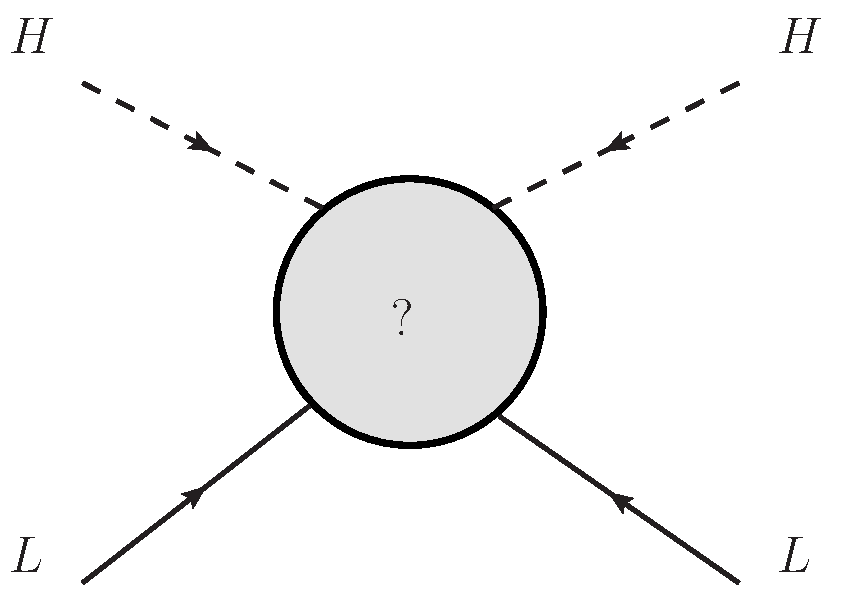
\includegraphics[scale=0.4]{fig5.pdf}
\end{center}
\caption{Schematic realization of the radiative see-saw mechanism at one-loop level. The new dark sector and consequently the DM particle is circling in the loop.}
\label{fig:see-saw-one-loop}
\end{figure} 
%
This realization of the $d=5$ Weinberg operator is diagrammatically shown in Fig.~\ref{fig:see-saw-one-loop}. 
For a complete diagrammatically and systematic study of the $d=5$ Weinberg operator at one-loop level see the Ref.~\cite{Bonnet:2012kz}.  
In particular, in this thesis, one specific realization of a well-motivated DM model is studied which will be described in the next chapter.

As a final comment and motivation, it is important to keep in mind that at one-loop level, the neutrino masses are approximately given by 
%
\begin{align}
m_{\nu}\propto 
\dfrac{\langle H^0\rangle ^2 }{\Lambda} \times \left(\dfrac{\epsilon}{16\pi^2}\right) \,,
\end{align}
%
where $\epsilon$ expresses symbolically the loop suppression. 
Therefore, the small neutrino masses are explained by the loop suppression and by the scale of the new physics.  See, for example, the see-saw radiative model described in~\cite{Ma:2006km}.



% Parts/Chapters
%	\part{Part A}
\chapter{Introduction to the singlet-doublet fermion DM model}
%
\InitialCharacter{T}he singlet-doublet fermion dark matter model (SDFDM) is introduced in this chapter.  
Its features are described in detail focusing in the contributions to the electroweak precision tests parameters, 
the Higgs and the $Z$ invisible decays, and its prospects for direct and indirect detection of dark matter. Also, it is described the implementation of this model and how the dark matter observables are computed using some high energy tools. At the end, it is shown how to enlarge the model with new reals scalar singlets in order to have radiative massive neutrinos.

\section{The SDFDM model}
\label{sec:model}
%
The SDFDM model has been previously studied in~\cite{D'Eramo:2007ga,Enberg:2007rp,Cohen:2011ec,Calibbi:2015nha,Abdallah:2015ter,Abe:2014gua}.
The particle content of the model consists of two $SU(2)_L$-doublets of
Weyl fermions $\widetilde{R}_u$, $R_d$  with opposite hypercharges and one singlet
Weyl fermion $N$ of zero hypercharge. 
All of them are odd under one imposed $Z_2$ symmetry, under which the SM
particles are even. 
The new particle content is summarized in Table~\ref{tab:partcont}.
%
\begin{table}
  \centering
  \begin{tabular}{|l|l|l|l|}
    \hline  
    Symbol     & $\left( SU(2)_L, U(1)_Y \right)$ & $Z_2$ & \text{Spin}\\ \hline
    $N$  & $(1,0)$ & $-$ & 1/2\\
     $\widetilde{R}_u$, & $(2, +1/2)$ & $-$ & 1/2\\ 
     $R_d$ & $(2, -1/2)$ & $-$ & 1/2\\ \hline
  \end{tabular}
  \caption{New $Z_2$-odd Weyl fermions in the SDFDM model.}
  \label{tab:partcont}
\end{table}
%
The most general $Z_2$-invariant Lagrangian is given by
\begin{align}
\label{eq:lt13A}
 \mathcal{L}= &\mathcal{L}_{\text{SM}}+\left[\mathcal{L}_{\text{Kin}}+ M_D \epsilon_{ab}R^a_d \widetilde{R}^b_u-\tfrac{1}{2}M_N NN-\lambda_d\, \epsilon_{ab}H^a R_d^b N-\lambda_u \epsilon_{ab}\widetilde{H}^a \widetilde{R}_u^b N+\text{h.c} \right]\,,
\end{align}
where
\begin{align}\label{eq:weyl-doublets}
  R_{d}=&
  \begin{pmatrix}
    \psi_{L}^{0}\\
    \psi_{L}^{-}
  \end{pmatrix}
&  
\widetilde{R}_{u}=&
  \begin{pmatrix}
   - \left( \psi_{R}^{-} \right)^{\dagger}\\
     \left(\psi_{R}^{0}\right)^{\dagger}
  \end{pmatrix}\,,
\end{align}
and $H=1/\sqrt{2} \begin{pmatrix}-iG^+ & h+v+iG^0\end{pmatrix}^{\operatorname{T}}$ is the SM Higgs doublet with $\widetilde{H}=i\sigma_2H^*$. 

In general, this model has four complex parameters ($-M_D, M_N, \lambda_u, \lambda_d$) of which
three  can be chosen reals with a redefinition of the fermion fields $N$, $R_d$ and $\widetilde{R}_{u}$. 
Therefore, in this work the three parameters  $-M_D$, $M_N,$ and $\lambda_u$ are chosen to be reals and positives. 
The last parameter $\lambda_d$ can be complex, but it was chosen real in order to avoid CP violation~\cite{Abe:2014gua}. 

Expanding the Lagrangian~\eqref{eq:lt13A} is obtained
\begin{align}
\label{eq:lt13a-expanded}
\mathcal{L}  \supset \, & \mathcal{L}_{\text{Kin}}+M_D(R_d^1\widetilde{R}_u^2-R_d^2\widetilde{R}_u^1)-\tfrac{1}{2}M_N NN
-\lambda_d(H^1R_d^2-H^2R_d^1)N-\lambda_u(\widetilde{H}^1R_u^2-\widetilde{H}^2R_u^1)N+\text{h.c}\nonumber \\
=\,& \mathcal{L}_{\text{Kin}}+M_D(\psi_L^0{\psi_{R}^0 }^{\dagger}+\psi_L^-{\psi_{R}^- }^{\dagger})-\tfrac{1}{2}M_N NN
+\dfrac{\lambda_d (h+v)}{\sqrt{2}}\psi_L^0N - \dfrac{\lambda_u (h+v)}{\sqrt{2}}{\psi_R^0}^{\dagger}N +\text{h.c}\nonumber\\
=\,& \mathcal{L}_{\text{Kin}}+\left[M_D\psi_L^0{\psi_{R}^0 }^{\dagger}-\tfrac{1}{2}M_N NN + \dfrac{\lambda_d v}{\sqrt{2}}\psi_L^0N - \dfrac{\lambda_u v}{\sqrt{2}}{\psi_R^0}^{\dagger}N\right]
+ M_D\psi_L^-{\psi_{R}^- }^{\dagger}
\nonumber\\ & 
+ \dfrac{h}{\sqrt{2}}\left(\lambda_d\psi_L^0N - \lambda_u{\psi_R^0}^{\dagger}N\right)+\text{h.c}.
%
\end{align}
%
Therefore, the $Z_2$-odd fermion spectrum in this model is composed of a
charged Dirac fermion $X^{\pm}=(\psi^{\pm}_L,\, \psi^{\pm}_R)^T$ with a tree
level mass $m_{X^\pm}=-M_D$, and three Majorana fermions $X_i^0$ $(i=1,2,3)$ that arise from
the mixture between the two neutral parts of the $SU(2)_L$ doublets and
the singlet fermion, i.e. between $\psi_L^0, \, {\psi_R^0}^{\dagger}$ and $N$. This spectrum will be discussed in the next section.






%%%%%%%%%%%%%%%%%%%%%%%%%%%%%%%%%%%%%%%%%%%%%%%%%%%%%%%%%%%%%%%%%%%%%%%%%%%%%%%%%%%%%%%%%%%%%%%%%%%%%%
\subsection{Neutral mass spectra}
%
Defining the fermion basis through the vector
\begin{align}
\label{eq:vecgauge}
\boldsymbol{\Xi}^{0}=
\begin{pmatrix}
N & R_d^1 & \widetilde{R}_u^2   
\end{pmatrix}^{\operatorname{T}}=
\begin{pmatrix}
N & \psi_L^0 & \psi_R^{0\dagger}
\end{pmatrix}^{\operatorname{T}},
\end{align} 
the mass terms in the Lagrangian~\eqref{eq:lt13a-expanded} can be written as
\begin{align}
\label{eq:neutral_lagrangian}
\mathcal{L}_{\Xi}
=& \left[ M_D\psi_L^0{\psi_{R}^0 }^{\dagger}-\tfrac{1}{2}M_N NN
+\dfrac{\lambda_d v}{\sqrt{2}}\psi_L^0N 
- \dfrac{\lambda_u v}{\sqrt{2}} {\psi_R^0}^{\dagger}N\right] +\text{h.c}\nonumber\\
=&-\dfrac{1}{2}\bigg[M_N NN - M_D(\psi_L^0{\psi_{R}^0 }^{\dagger}+{\psi_{R}^0 }^{\dagger}\psi_L^0)
-\dfrac{\lambda_d v}{\sqrt{2}}(\psi_L^0N+N\psi_L^0) 
+\dfrac{\lambda_u v}{\sqrt{2}} ({\psi_R^0}^{\dagger}N+N{\psi_R^0}^{\dagger})\bigg] +\text{h.c}
\nonumber\\
  =&-\frac{1}{2}
\boldsymbol{\Xi}^{0\operatorname{T}}
\mathbf{M}^{\chi}\boldsymbol{\Xi}^0
+\text{h.c}\,,
\end{align}
where
\begin{align}
\label{eq:Mchis}
  \mathbf{M}^{\chi}=\begin{pmatrix}
  M_N                 &-\dfrac{\lambda_d v}{\sqrt{2}}&\dfrac{\lambda_u v}{\sqrt{2}}\\
-\dfrac{\lambda_d v}{\sqrt{2}} &  0                  & -M_D\\
\dfrac{\lambda_u v}{\sqrt{2}}&  -M_D                &  0  \\
\end{pmatrix}\,.
\end{align} 
By defining
%%%%%%%%%%%%%%%%%%%%%%%%%%%%%%%%%%%%%%%%%%%%%%%%%%%%%%%%
\begin{align}
  \label{eq:etabeta}
m_{\lambda}=&  \frac{\lambda v }{\sqrt{2}}\,,&
  \lambda=&\sqrt{\lambda_u^2+\lambda_d^2}\,,&
  \tan\beta=&\frac{\lambda_u}{\lambda_d}\, ,
\end{align}
the neutral fermion mass matrix is given by
\begin{align}
\label{eq:Mchi}
  \mathbf{M}^{\chi}=\begin{pmatrix}
 M_N                 &-m_{\lambda}\cos\beta&m_{\lambda}\sin\beta\\
-m_{\lambda}\cos\beta &  0                  & -M_D\\
m_{\lambda}\sin\beta&  -M_D                &  0  \\
\end{pmatrix}\,,
\end{align}
%
which follow the same
convention of the bino-higgsino sector in the neutralino mass matrix of the
minimal supersymmetric standard model (MSSM)~\cite{Martin:2012us}. 
This convention facilitates the comparison between the present study and previous analysis
regarding the bino-higgsino DM limit of the MSSM. 
Such a limiting scenario occurs in the MSSM when the winos are decoupled from the spectrum and is accommodated within the SDFDM model when
$m_\lambda=m_Z\sin\theta_W$ ($\lambda=g'/\sqrt{2}$).










%%%%%%%%%%%%%%%%%%%%%%%%%%%%%%%%%%%%%%%%%%%%%%%%%%%%%%%%%%%%%%%%%%%%%%%%%%%%%%%%%%%%%%%%%%%%%%%%%
\subsubsection{Neutral mass eigenstates}
In order to get the physics eigenstates, this mass matrix needs to be diagonalized,
in such a way that the fermion mass eigenstates $\mathbf{X}=(\chi_1^0,\chi_2^0,\chi_3^0)^T$ are obtained through the rotation
matrix $\mathbf{N}$\footnote{In~\cite{Horiuchi:2016tqw} was used $\mathbf{U}$ instead $\mathbf{N}$. The equivalence is $\mathbf{N}=\mathbf{U}^T$.} as 

\begin{align}
\label{eq:rotation}
\boldsymbol{\Xi}^0 = \begin{pmatrix}N\\ \psi_L^0 \\ (\psi_R^0)^\dagger\end{pmatrix}= 
\mathbf{N}\begin{pmatrix}\chi_1^0\\ \chi_2^0 \\ \chi_3^0\end{pmatrix}= \mathbf{N}\mathbf{X} \,,
\end{align}
such that

\begin{align}
\label{eq:chidiag}
 \mathbf{N}^{\operatorname{T}}\mathbf{M}^\chi \mathbf{N}=\mathbf{M}^\chi_\text{diag}\,,
\end{align}
%
with $\textbf{M}^\chi_{\text{diag}}=\operatorname{Diag}(m^\chi_1,m^\chi_2,m^\chi_3)$ and $m^\chi_n$ being the corresponding physical masses (not mass ordering is implied). 
Even more, CP invariance is assumed and therefore $\mathbf{N}$ can be chosen real. By using the neutral Lagrangian~\eqref{eq:neutral_lagrangian} and the Eq.~\eqref{eq:rotation} for the rotation, 
it is possible to get the following expressions for the masses
%
\begin{align}
\label{eq:masses_diag}
m^\chi_1=&\tfrac{1}{2}M_NN_{11}^2 - M_D N_{21}N_{31}-\dfrac{\lambda_dv}{\sqrt{2}}N_{11}N_{21}+\dfrac{\lambda_uv}{\sqrt{2}}N_{11}N_{31}\\
m^\chi_2=&\tfrac{1}{2}M_NN_{12}^2 - M_D N_{22}N_{32}-\dfrac{\lambda_dv}{\sqrt{2}}N_{12}N_{22}+\dfrac{\lambda_uv}{\sqrt{2}}N_{12}N_{32}\\
m^\chi_3=&\tfrac{1}{2}M_NN_{13}^2 - M_D N_{23}N_{33}-\dfrac{\lambda_dv}{\sqrt{2}}N_{13}N_{23}+\dfrac{\lambda_uv}{\sqrt{2}}N_{13}N_{33} \,.
\end{align}
%
The analytical diagonalization of the neutral fermion mass matrix is
carried out in Appendix~\ref{sec:analyt-form-mass}. 
It is useful and convenient in some analysis to have approximate expressions in
the limit of small fermion mixing ($m_\lambda\ll M_D,M_N)$. For instance,
expanding the analytical expressions for the eigensystem of
Eq.~\eqref{eq:chidiag} given in Appendix~\ref{sec:analyt-form-mass}
up to order $m_{\lambda}^2$, the fermion masses are given by
%
\begin{align}
\label{eq:ml2}
m^\chi_1=&M_{N} + \frac{M_{D} \sin{\left (2 \beta \right )} + M_{N}}{M_{N}^{2}- M_{D}^{2} }\, m_{\lambda}^{2}+\mathcal{O}\left( m_{\lambda}^4 \right) \nonumber\\
m^\chi_2=&M_{D} + \frac{ \sin(2 \beta ) + 1}{2 \left( M_{D} -  M_{N} \right)}\,m_{\lambda}^{2}+\mathcal{O}\left( m_{\lambda}^4 \right) \nonumber\\
m^\chi_3=&- M_{D} + \frac{ \sin(2 \beta ) - 1}{2 \left( M_{D} + M_{N} \right) }\,m_{\lambda}^{2}+\mathcal{O}\left( m_{\lambda}^4 \right)\,.
\end{align}
Approximate expressions for the mixing matrix are also given in the Appendix~\ref{sec:analyt-form-mass}.











%%%%%%%%%%%%%%%%%%%%%%%%%%%%%%%%%%%%%%%%%%%%%%%%%%%%%%%%%%%%%%%%%%%%%%%%%%%%%%%%%%%%%%%%%%%%%%%%%%%%%%%%%%%
\subsection{The interaction Lagrangian}
%
According to the Lagrangian Eq.~\eqref{eq:lt13a-expanded}, the interaction terms, and the free-fermion Lagrangian  are given by
%
\begin{align}
\label{eq:lint1}
\mathcal{L} \, \supset \, &\mathcal{L}_{\text{Kin}}
- \dfrac{h}{\sqrt{2}}\left(-\lambda_d\psi_L^0N + \lambda_u{\psi_R^0}^{\dagger}N\right)+\text{h.c}\nonumber\\
= \, & \dfrac{i}{2}\left(N^{\dagger}\overline{\sigma}^{\mu}\partial_{\mu}N 
+  R_d^{\dagger}\overline{\sigma}^{\mu}D_{\mu}R_d 
+  \widetilde{R}_u^{\dagger}\overline{\sigma}^{\mu}D_{\mu}\widetilde{R}_u \right)
- \dfrac{h}{\sqrt{2}}\left(-\lambda_d\psi_L^0N + \lambda_u{\psi_R^0}^{\dagger}N+\text{h.c}\right)\,,
\end{align}
%
where $D_{\mu}$ is the SM covariant derivative. 

Although, this Lagrangian is written in terms of Weyl spinors,
in the  Appendix~\ref{sec:lag-interaction}
the Majorana spinors $X_i^0$ and the Dirac spinor $X^{\pm}$  are constructed as
\begin{align}
X_i^0=\begin{pmatrix}
(\chi_{i}^0)_\alpha \\ (\chi_i^{0\dagger})^{\dot{\alpha}}
\end{pmatrix}
=\begin{pmatrix}
N_{ji}\,\boldsymbol{\Xi}^{0}_j \\
N_{ji}^{\dagger}\,\boldsymbol{{\Xi}^{\dagger}}^{0}_j
\end{pmatrix}
\hspace{1.5 cm}
X^{\pm}=\begin{pmatrix}
\chi^{\pm}_{\alpha} \\ {\chi^{\mp}}^{\dagger\dot{\alpha}}
\end{pmatrix}
=\begin{pmatrix}
\psi_L^{\pm} \\
{\psi_R^{\mp}}^{\dagger}
\end{pmatrix}\,,
\end{align}
%
and it is shown that the interaction Lagrangian in terms of four-component spinors is given by
%
\begin{align}
\label{eq:lint4}
\mathcal{L}_{\text{Int}}= & 
-\dfrac{g}{\sqrt{2}}\left(\bar{X}^-\slashed{W}\left(N_{2i}P_L-N_{3i}P_R\right)X_i^0 + \text{h.c}\right)
+ \dfrac{g}{4\cos\theta}\bar{X}_i^0\slashed{Z}\left(N_{2i}N_{2j}-N_{3i}N_{3j}\right)\gamma^5X_j^0 \nonumber\\
+& g\left(\dfrac{2\cos^2\theta_W-1}{2\cos\theta_W}\right)
\bar{X}^-\slashed{Z}X^-
-e\bar{X}^-\slashed{A}X^- 
-\dfrac{1}{\sqrt{2}}h\bar{X}_i^0\left(-\lambda_dN_{2i}N_{1j} + \lambda_uN_{3i}N_{1j}\right)X_j^0\,.
\end{align}
%
In particular, the interaction of the DM particle $X_i^0$ with the $W$, $Z$ and $h$ SM gauge boson is given by 
%
\begin{align}
\mathcal{L^{\chi}}_{\text{Int}}=
-\bar{X}^-\slashed{W}c_{WXX_i}X_i^0
-c_{ZX_iX_j}\bar{X}_i^0\slashed{Z}\gamma^{5}X_j^0
-c_{hX_iX_j}h\bar{X}_i^0X_j^0 \,,
\end{align}
where 
\begin{align}
c_{WXX_i}=& \dfrac{g}{\sqrt{2}}\left(N_{2i}P_L-N_{3i}P_R\right)  \label{eq:cWXXi}\\
c_{ZX_iX_j}=&\frac{g}{4\cos\theta_W}(N_{3i}N_{3j}-N_{2i}N_{2j}) \label{eq:cZXiXj}\\
%problema en el orden
c_{hX_iX_j}=&\frac{1}{\sqrt{2}}(-\lambda_dN_{2i}N_{1j}+\lambda_uN_{3i}N_{1j})\label{eq:cHXiXj}\,,
\end{align}
%
which it is in agreement with the Ref.~\cite{Abdallah:2015ter}.
 
As is usually done, we denote the lightest stable particle in our model by 
$\chi^0\,$~\footnote{Actually, it is the lightest stable Majorana four-component spinor $X_i^0$, which will be denote as $\chi^0$ for simplicity.}, whose couplings with the $Z$ and $h$ gauge bosons can explicitly written as~\cite{Calibbi:2015nha}
\begin{align}
c_{Z\chi^0\chi^0}&=-\frac{m_Z\lambda^2v(m_{\chi^0}^{2}-M_D^2)\cos2\beta}{2(m_{\chi^0}^{2}-M_D^2)^2+\lambda^2v^2\left(2\sin2\beta m_{\chi^0} M_D+m_{\chi^0}^{2}+M_D^2\right)} \,,\label{eq:cZXX}\\
c_{h\chi^0\chi^0}&=-\frac{(M_D\sin 2\beta+m_{\chi^0})\lambda^2v}{M_D^2+\lambda^2v^2/2+2M_N\,m_{\chi^0}-3m_{\chi^0}^{2}}\label{eq:cHXX}\,.
\end{align}










%%%%%%%%%%%%%%%%%%%%%%%%%%%%%%%%%%%%%%%%%%%%%%%%%%%%%%%%%%%%%%%%%%%%%%%%%%%%%%%%%%%%%%%%%%%%%%%%%%%%%%%%%%%%
\section{Invisible decays}
%
This model has a new contribution to the Higgs and $Z$ gauge bosons invisible decay fraction. Those are given by
%
\begin{align}
\Gamma(h \rightarrow \chi^0\chi^0) = \dfrac{m_h}{4\pi}\bigg(1-\dfrac{4m_{\chi^0}^2}{m_h^2}\bigg)^{3/2}|c_{h\chi^0\chi^0}|^2
\end{align}
and
\begin{align}
\Gamma(Z \rightarrow \chi^0\chi^0) = \dfrac{m_Z}{6\pi}\bigg(1-\dfrac{4m_{\chi^0}^2}{m_Z^2}\bigg)^{3/2}|c_{Z\chi^0\chi^0}|^2 \,.
\end{align}
%
Therefore, in order to do a good and viable study in this model, it is necessary to restrict the parameter space to all the points that have a BR($h\rightarrow\chi^0\chi^0) < 0.19$ to $2\sigma$ in accord with the LCH an ILC prospects~\cite{Bechtle:2014ewa} and $\Gamma(Z\rightarrow\chi^0\chi^0) \lesssim 3$ MeV in accord with LEP~\cite{ALEPH:2005ab}.









%%%%%%%%%%%%%%%%%%%%%%%%%%%%%%%%%%%%%%%%%%%%%%%%%%%%%%%%%%%%%%%%%%%%%%%%%%%%%%%%%%%%%%%%%%%%%%%%%%%%%%%%%%%%
\section{Electroweak precision observables (EWPO) }
\label{sec:EWPO}
%%%%%%%%%%%%%%%%%%%%%%%%%%% PLOT STU  %%%%%%%%%%%%%%%%%%%%%%%%%%%
\begin{figure}[h]
\begin{center}
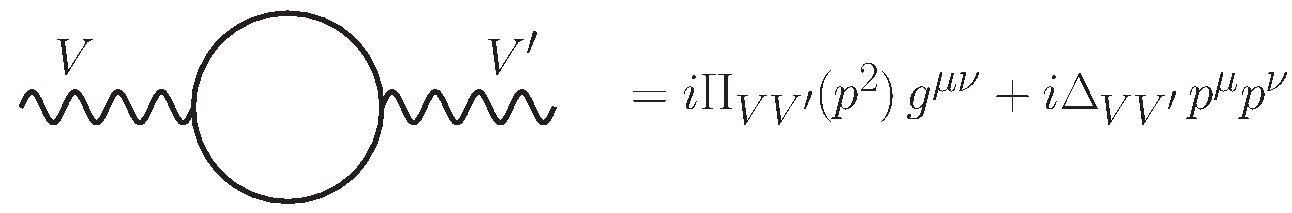
\includegraphics[scale=0.5]{fig1.pdf}
\end{center}
\caption{Gauge boson two-point  functions.}
\label{fig:STU-propagator}
\end{figure}
%%%%%%%%%%%%%%%%%%%%%%%%%%%%%%%%%%%%%%%%%%%%%%%%%%%%%%%%%%%%%%%%%
The SDFM model presents new contributions to the electroweak precision observables (EWPO). 
The ($V = W,\gamma, Z$) gauge bosons  two-point functions shown in Fig.~\ref{fig:STU-propagator} are modified by the presence of the new $Z_2$-odd particles circulating in the loop. 
It gives a new contribution to the Peskin-Takeuchi $S$, $T$, $U$ parameters~\cite{PhysRevD.46.381}, which are defined as
%
\begin{align}
\label{eq:ST-definition}
S=&\dfrac{4s^2c^2}{\alpha}\left(\dfrac{\Pi_{ZZ}(m_Z^2)
-\Pi_{ZZ}(0)}{m_Z^2}-\dfrac{c^2-s^2}{sc}\dfrac{\Pi_{Z\gamma}(m_Z^2)}{m_Z^2}
-\dfrac{\Pi_{\gamma\gamma}(m_Z^2)}{m_Z^2}\right)\\
T=&\dfrac{1}{\alpha}\left(\dfrac{\Pi_{WW}(0)}{m_W^2}-\dfrac{\Pi_{ZZ}(0)}{m_Z^2}\right)\\
U=&\dfrac{4 s^2}{\alpha}\left(\Pi'_{WW}(0)-c^2\,\Pi'_{ZZ}(0)-2\,sc\,\Pi'_{Z\gamma}(0)-s^2\Pi'_{\gamma\gamma}(0)\right) \,,
\end{align}
with $s=\sin\theta_W$ and $c=\cos\theta_W$ \footnote{The definition for the $\Pi$ functions can be found in the Refs.~\cite{Abe:2014gua} and \cite{D'Eramo:2007ga}.}.  
%
Actually, the only important parameters are $S$ and $T$. The $U$ parameter is not useful in practice because its contribution from most new physics models is very small. It can be shown that $U$ actually parametrizes the coefficient of a dimension-eight operator, while $S$ and $T$ can be represented as a dimension-six operator. 
%
Something important is that a charge conjugation symmetry ($\tilde{R}_u\leftrightarrow R_d$) in the Lagrangian~\eqref{eq:lt13A} 
is obtained when $\lambda_u=|\lambda_d|$ and this causes a vanishing DM coupling with the $Z$ gauge boson ($N_{21}=N_{31}$ in the Eq.\eqref{eq:cZXiXj}). Even more, due to this custodial symmetry, the new contribution to the $T$ parameter vanishes for this particular case. 

For the analysis carried out in this work, it has been used the correction $\Delta S$ and $\Delta T$  reported in the Ref.~\cite{D'Eramo:2007ga}~\footnote{ A crosscheck has been done with the Ref.~\cite{Abe:2014gua}.}. 
Those are given by
%
\begin{eqnarray}
\Delta T & = & \sum_{i=1}^{3}\left[
\left(V_{1i}\right)^{2}\widetilde{A}\left(M,m_{i}\right)+
\left(V_{2i}\right)^{2}\widetilde{A}\left(M,-m_{i}\right)\right]
\nonumber\\ & & -\frac{1}{2}\sum_{i,j=1}^{3}
\left(V_{1i}V_{2j}+V_{2i}V_{1j}\right)^{2}\widetilde{A}\left(m_{i},-m_{j}\right) \,,
\end{eqnarray}
%
\begin{equation}
\Delta S =   \frac{1}{2}\sum_{i,j=1}^{3}
\left(V_{1i}V_{2j}+V_{2i}V_{1j}\right)^{2}\widetilde{F}\left(m_{i},-m_{j}\right)-\widetilde{F}\left(\mu,\mu\right) \,,
\end{equation}
where
\begin{equation}
\widetilde{A}\left(m_{1},m_{2}\right)\equiv
\frac{1}{2\alpha_{em}v^{2}}\Pi\left(0\right) \,,
\end{equation}
%
\begin{equation}
\widetilde{F}\left(m_{1},m_{2}\right)\equiv 4\pi
\Pi^{'}\left(0\right) \,,
\end{equation}
%
\begin{eqnarray}
\Pi(0) & = & \frac{1}{16\pi^{2}}\left[
\left(m_{1}-m_{2}\right)^{2}\ln\frac{\Lambda^{4}}{m_{1}^{2}m_{2}^{2}}-2m_{1}m_{2}\right.
\nonumber\\ & &
+\left.\frac{2m_{1}m_{2}\left(m_{1}^{2}+m_{2}^{2}\right)-m_{1}^{4}-m_{2}^{4}}{m_{1}^{2}-m_{2}^{2}}
\ln\frac{m_{1}^{2}}{m_{2}^{2}}\right] \,,
\end{eqnarray}
%
\begin{eqnarray}
\Pi^{'}(0) & = & \frac{1}{24\pi^{2}}\left[
-\ln\frac{\Lambda^{4}}{m_{1}^{2}m_{2}^{2}}-
\frac{m_{1}m_{2}\left(3m_{1}^{2}-4m_{1}m_{2}+3m_{2}^{2}\right)}{\left(m_{1}^{2}-m_{2}^{2}\right)^{2}}\right.
{}\nonumber\\ & &
{}+\left.\frac{m_{1}^{6}+m_{2}^{6}-3m_{1}^{2}m_{2}^{2}\left(m_{1}^{2}+m_{2}^{2}\right)+6m_{1}^{3}m_{2}^{3}}
{\left(m_{1}^{2}-m_{2}^{2}\right)^{3}}\ln\frac{m_{1}^{2}}{m_{2}^{2}}\right] \,.
\end{eqnarray}
%
These expressions are valid for Dirac particles and for Majorana fermions with an extra factor of two and with $\Lambda$ the cutoff of the loop integral which
disappears at the end of the computation.

To be compatible with the parametrization used in the Eq.~\eqref{eq:Mchis}, the next identification was carry out: $M\to -M_D$ , $\mu\to -2M_N$ , $\alpha=\frac{\lambda_u+\lambda_d}{2}$ , $\beta'=\frac{\lambda_u-\lambda_d}{2}$ and the $V_{ij}$ coefficients were obtained after the diagonalization of the matrix
%
\begin{equation}
 \mathbf{M}^{\chi}=\left(
\begin{array}{ccc}
M & 0 & -\beta' v \\
0 & -M & -\alpha v\\
-\beta' v & -\alpha v & -2 \mu
\end{array} \right) \,,
\end{equation}
which is the neutral fermion mass matrix obtained in the basis used in the Ref.~\cite{D'Eramo:2007ga}.

%
%%%%%%%%%%%%%%%%%%%%%%%%%%% PLOT EDM   %%%%%%%%%%%%%%%%%%%%%%%%%%%
\begin{figure}[h]
\begin{center}
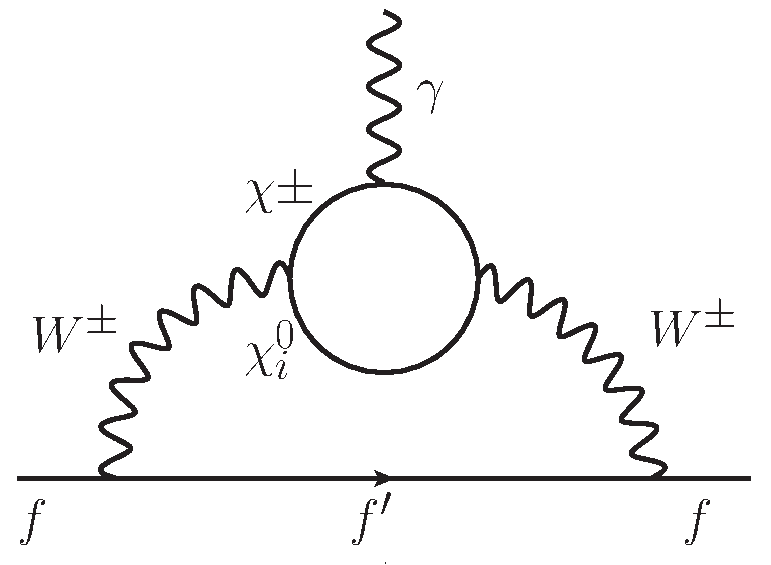
\includegraphics[scale=0.4]{fig2.pdf}
\end{center}
\caption{Contribution to the electric dipole moment (EDM) of a fermions $f$ in the SM.}
\label{fig:EDM}
\end{figure}
%%%%%%%%%%%%%%%%%%%%%%%%%%%%%%%%%%%%%%%%%%%%%%%%%%%%%%%%%%%%%%%%%
%

As a final comment, the contributions to the electric dipole moment (EDM) of the particles in the SM, which is the process shown in Fig.~\ref{fig:EDM}
happens when the Yukawa couplings $\lambda_u , \lambda_d$ are complex numbers. However, this work is not focused on that direction because the couplings were chosen as real numbers. Those issues were discussed in the Ref.~\cite{Abe:2014gua}.










%%%%%%%%%%%%%%%%%%%%%%%%%%%%%%%%%%%%%%%%%%%%%%%%%%%%%%%%%%%%%%%%%%%%%%%%%%%%%%
\section{The dark matter abundance $\Omega h^2$ }
\label{sec:abundance}
%
%%%%%%%%%%%%%%%%%%%%%%%% PLOT Fig8. %%%%%%%%%%%%%%%%%%%%%%%%%%%
\begin{figure}[h]
\begin{center}
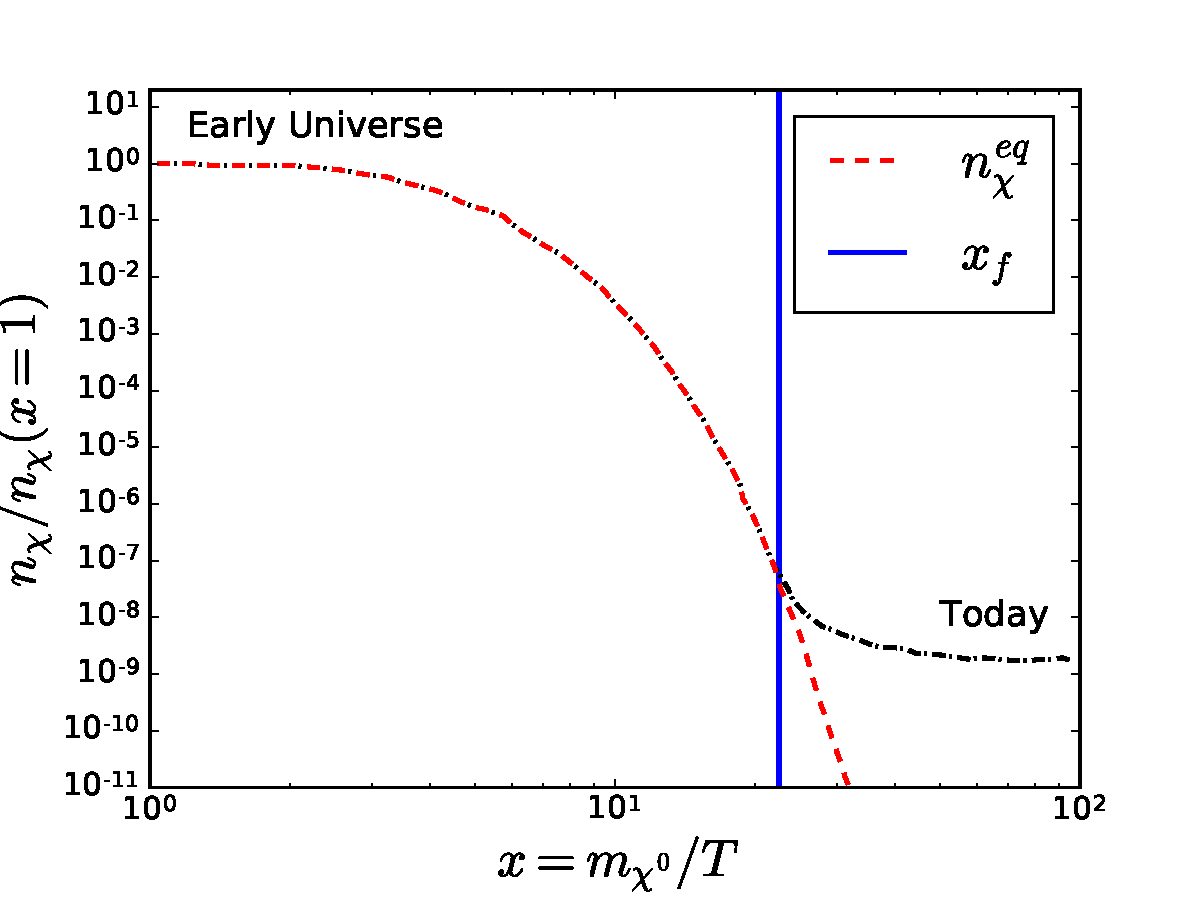
\includegraphics[scale=0.45]{freeze-out.pdf}
\end{center}
\caption{A DM number density illustration which follows the equilibrium density ($n_{\chi}^{\text{eq}}$) to the point $x_f$ (``freeze-out"). After that it remains constant to today.}
\label{fig:freeze-out}
\end{figure}
%%%%%%%%%%%%%%%%%%%%%%%%%%%%%%%%%%%%%%%%%%%%%%%%%%%%%%%%%%%%%%%%%
%
The DM abundance for the SDFDM model can be computed using the standard analysis for a cold relic density decoupled in the early Universe. In this picture, the evolution of the number density of the DM particles $n_{\chi}$ is governed by the Boltzmann equation~\cite{Kolb:1990vq}
\begin{align}
\dfrac{dn_{\chi}}{dt}+3Hn_{\chi}=&-\langle \sigma v \rangle \left[n_{\chi}^2-(n_{\chi}^{\text{eq}})^2\right]\,,
\end{align}
where $H$ is the Hubble parameter that characterize the Universe's expansion, $n_{\chi}^{\text{eq}}$ is the number density when the DM particles are in equilibrium, i.e. when the DM particles are not decoupled in the early Universe and $\langle \sigma v \rangle$ is the thermal velocity averaged self-annihilation cross section.

The Boltzmann equation can be solved approximately when
the temperature dependence of the  $\langle \sigma v \rangle$ is parameterized as
%
\begin{align}
\langle\sigma v\rangle= &\, \sigma_0\, x^{-n}\,,
\end{align} 
%
where $\sigma_0$ is the cross section to zero temperature, $x=m_{\chi^0}/T$ and $n=0$ corresponds to the s-wave  contribution, $n=1$ to the p-wave, etc.

The idea of the concept of the relic density is shown in Fig.~\ref{fig:freeze-out}. In the early Universe the DM number density $n_{\chi}$ is approximately given by $n_{\chi}^{\text{eq}}$.
However, with the expansion of the Universe, the temperature drops below the mass of the DM particle and the reaction rate $\Gamma(\chi^0\chi^0\leftrightarrow \text{SM\, SM})$ gets slower than the expansion of the Universe and the $n_{\chi}^{\text{eq}}$ drops exponentially until a point called ``freeze-out" ($x_f=m_{\chi^0}/T_f$).
In this point, the reaction is not fast enough to hold the equilibrium and the DM particle is decoupled of the SM particles and its density remains constant to today.  
In general, the Boltzmann equation can be solved  before the ``freeze-out" when $n_{\chi}\approx n_{\chi}^{\text{eq}}$ and  after that,  when $n_{\chi}^{\text{eq}} \ll n_{\chi}$ and $n_{\chi}^{\text{eq}}$ can be neglected.
The complete solution is obtained by using the matching between last two solutions just at the `freeze-out" point.
Without entering in more details, this solution is given by~\cite{D'Eramo:2007ga}
%
\begin{align}
\Omega h^2  \approx & (n+1)\dfrac{x_f}{g_*^{1/2}}\dfrac{0.034\, \text{pb}}{\langle \sigma v_r\rangle} \,,
\end{align} 
where the variable $x_f$ at the ``freeze-out" is computed solving the equation
\begin{align}
x_f+(n+1)\log x_f \approx \log\left[0.038\left(n+1\right)\left(\dfrac{g}{g_*^{1/2}}\right)M_{p}\,m_{\chi^0}\,\sigma_{0}\right]\,,
\end{align} 
with $M_{p}=1.22 \times 10^{19}$ GeV the Planck mass.

These expressions were computed and checked using \textsc{micrOMEGAs 4.1.8}~\cite{Belanger:2014vza}. A good agreement was obtained for some special cases of the parameter space where the $\langle \sigma v \rangle$ is easily computed by hand. However, the numerical solution obtained with \textsc{micrOMEGAs} was used because it takes care of the complete $\langle \sigma v \rangle$ when the self-annihilation of DM takes place in all the possible final channels that will be described later. Even more,  \textsc{micrOMEGAs} takes care of difficult regions of the parameter space, for instance, the process of coannihilations and resonances~\cite{Griest:1990kh}. 












%%%%%%%%%%%%%%%%%%%%%%%%%%%%%%%%%%%%%%%%%%%%%%%%%%%%%%%%%%%%%%%%%%%%%%%%%%%%%%%%%%%%%%%%%%%%%%%%%%%%%%%%%%%%
\section{Model's implementation}
%
%%%%%%%%%%%%%%%%%%%%%%%% PLOT Fig8. %%%%%%%%%%%%%%%%%%%%%%%%%%%
\begin{figure}[h]
\begin{center}
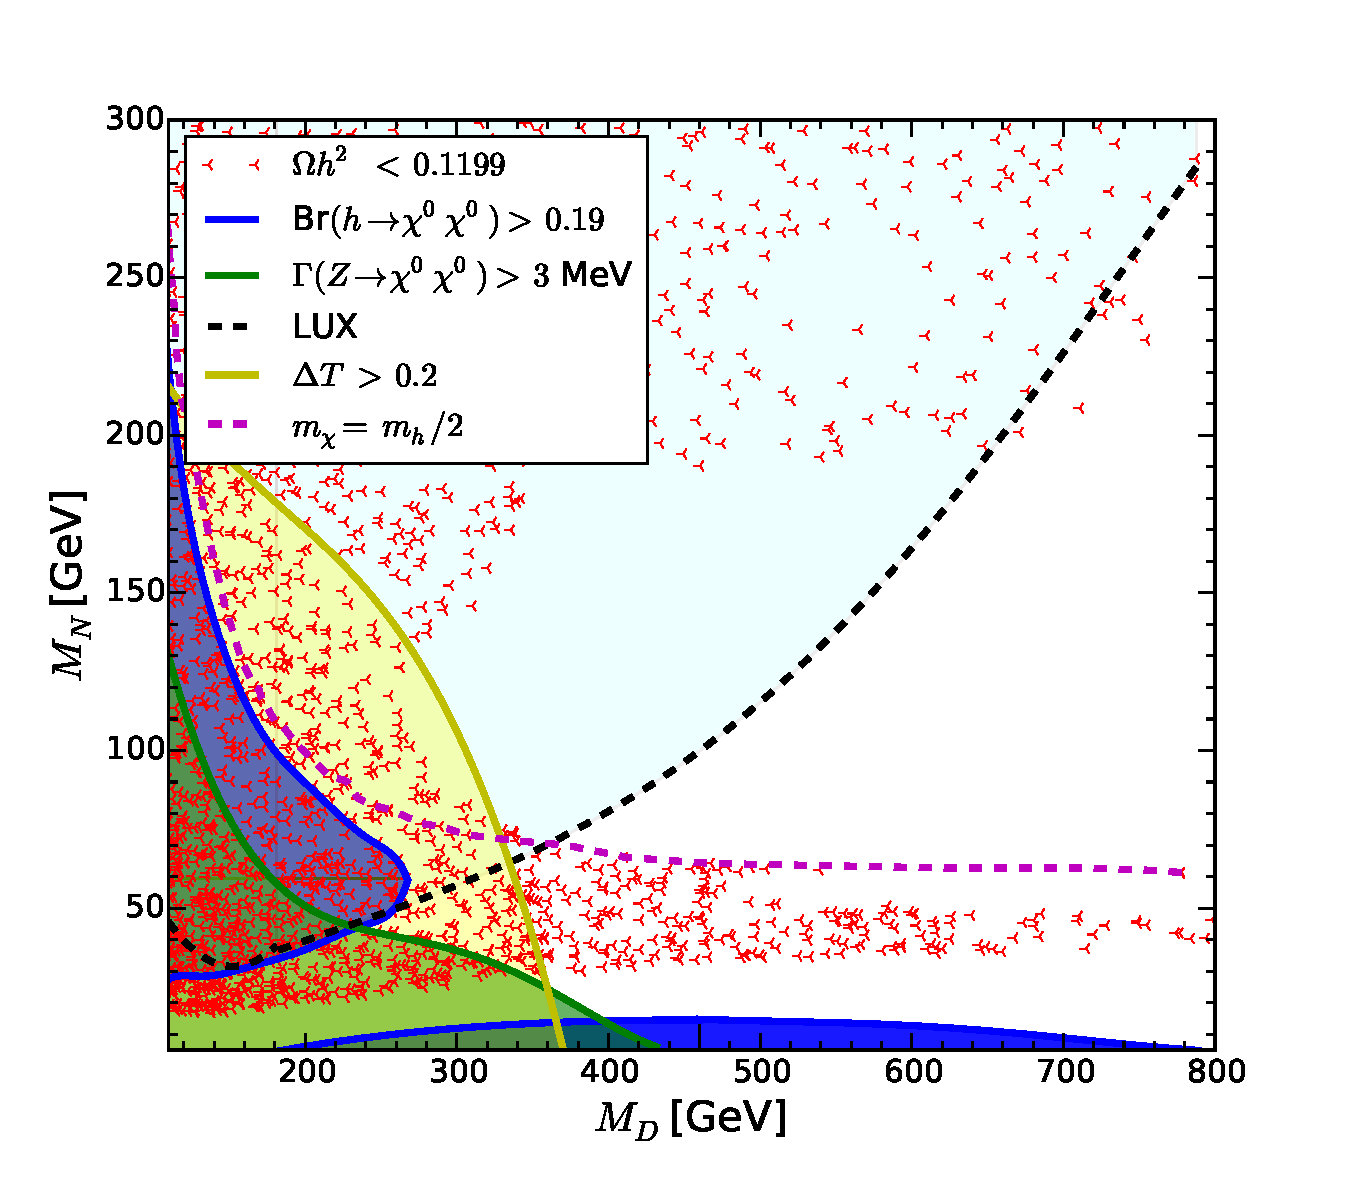
\includegraphics[scale=0.5]{fig8.pdf}
\end{center}
\caption{Constraints on the SDFDM model in the low mass region for $\lambda=1$ and $\tan\beta=-20$. Above the black dashed line: region exclude by LUX ($\sigma_{SI}$). Yellow: region excluded by EWPO. Green (Blue): region excluded by the $Z$ ($h$) invisible decay. The magenta dashed line corresponds to $m_{\chi^0}=m_h/2 $.}
\label{fig:fig8-1505.03867}
\end{figure}
%%%%%%%%%%%%%%%%%%%%%%%%%%%%%%%%%%%%%%%%%%%%%%%%%%%%%%%%%%%%%%%%%

The SDFDM model was implemented in \textsc{Feynrules 2.3}~\cite{Christensen:2008py} and a crosscheck was done using the \texttt{BSM-Toolbox}~\cite{Staub:2011dp} of \texttt{SARAH}~\cite{Staub:2008uz,Staub:2013tta}.
%
The first step was to reproduce some of the known results for this model. 
For that purpose, a benchmark point was taken in order to check the implementation.
For instance, Fig.8 of the Ref.~\cite{Calibbi:2015nha} that shows the behavior of the model for the specific case of $\lambda=1$ and $\tan\beta=-20$.
% 
We used the LUX-2013~\cite{Akerib:2013tjd}  limits for spin-independent cross section with nucleons
and we assumed that the DM  relic density saturates the Planck measurement $\Omega h^2=(0.1199 \pm 0.0027)$~\cite{Ade:2013zuv} at the $3\,\sigma$. 
The results are shown in Fig.~\ref{fig:fig8-1505.03867}.
There, the region above the black dashed line is excluded by LUX. In the same way, the green (blue) region is excluded by the $Z$ ($H$) invisible decay and the yellow region  is excluded by the correction to the EWPO parameters (we disagree with the Ref.~\cite{Calibbi:2015nha} by a factor two in the $\Delta T$ computation,
that factor takes into account that DM particles are Majorana fermions).
Note that the boundary of the region given by the red points reproduces the experimental value of  $\Omega h^2$, while the remaining white zones have an overabundance of the DM relic density.



 






%%%%%%%%%%%%%%%%%%%%%%%%%%%%%%%%%%%%%%%%%%%%%%%%%%%%%%%%%%%%%%%%%%%%%%%%%%%%%%
\section{Indirect detection }
\label{sec:indirec-detection}

%\subsection{DM self-annihilation channels}

\begin{figure}
\begin{center}
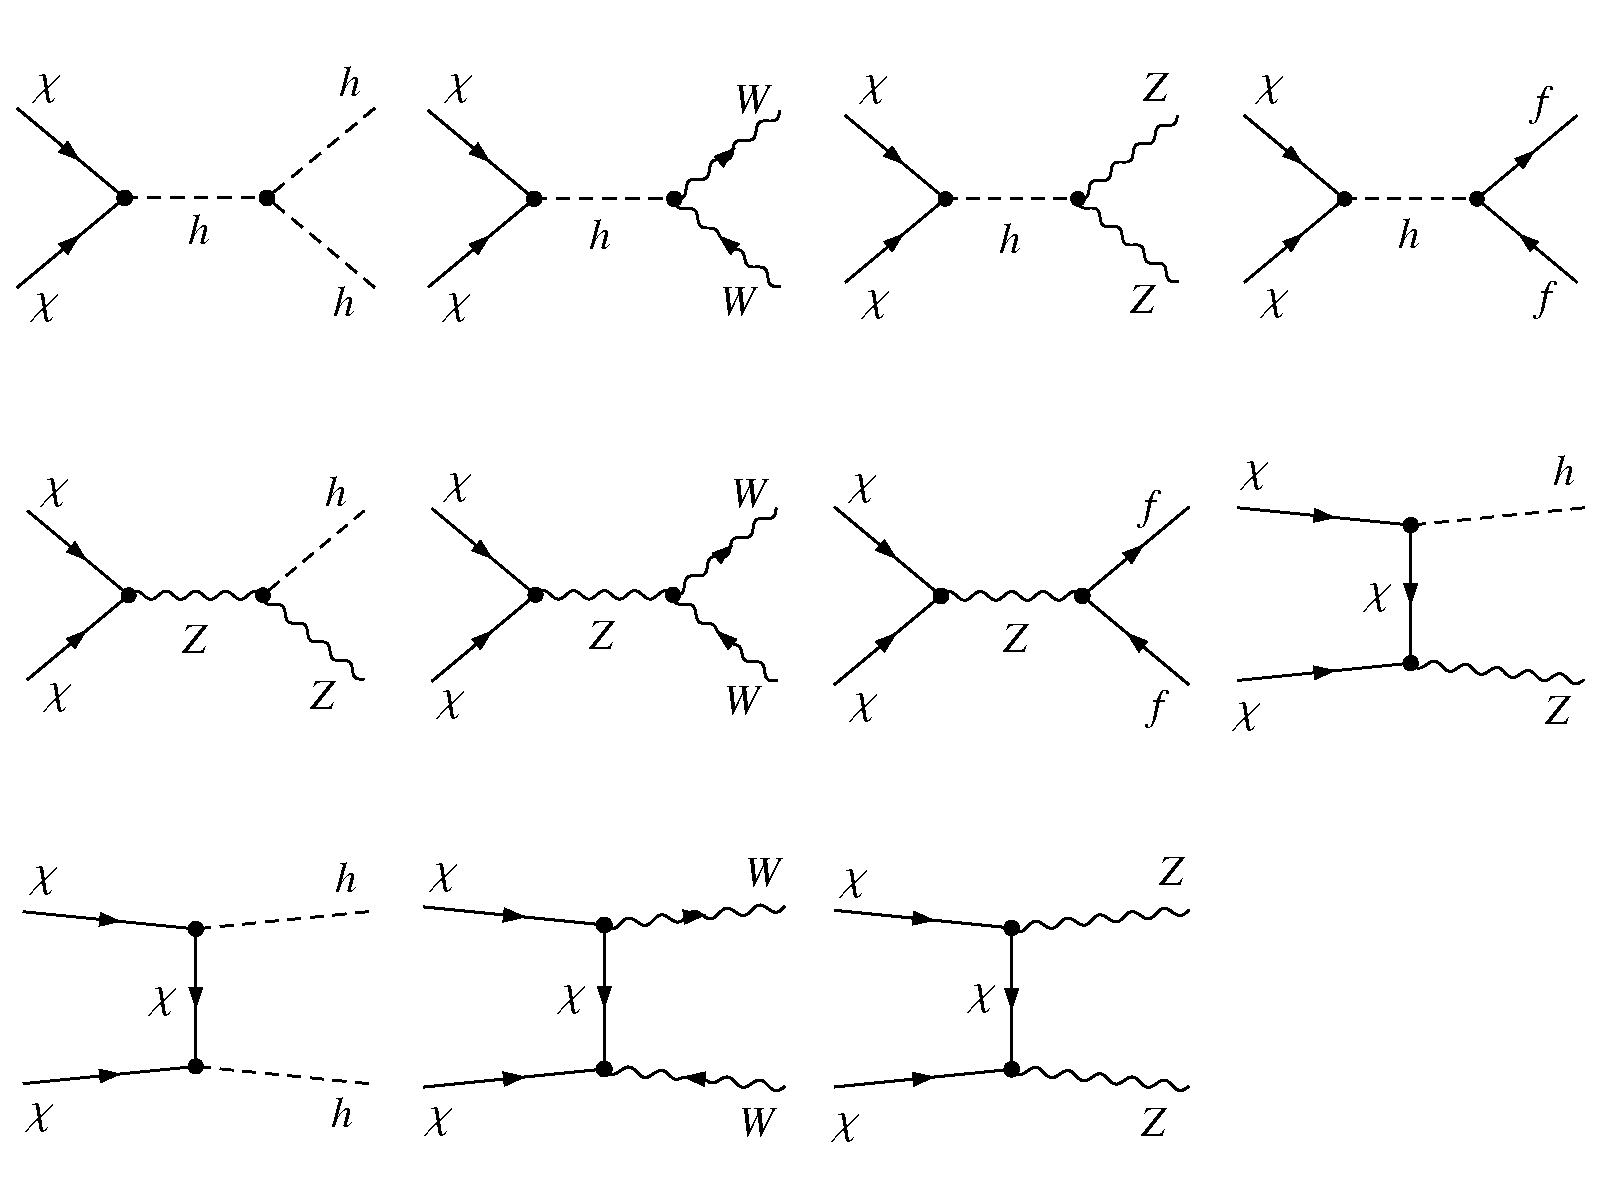
\includegraphics[scale=0.47]{XXtoSM}
\end{center}
\caption{Self-annihilation channels a tree level in the SDFDM model. The u-channels are not shown. They were generated using \textsc{FeynArts}~\cite{Hahn:2000kx}.}
\label{fig:self-channels}
\end{figure}

At tree level, the interaction between the DM and the SM sector is mediated by the $W$, $Z$ and $H$ gauge bosons.
In this model, DM particle ($\chi^0$) can self-annihilate into $\bar{f}f$, $ZZ$, $W^+W^-$ and $hh$ final states through  $s$-channel Higgs and $Z$ boson exchange and into $ZZ$, $W^+W^-$ states via $t$-channel $\chi_i^0$ and $\chi^{\pm}$ exchange. Annihilation into a mixture of weak gauge bosons $Zh$ is also possible through the exchange of a $\chi_i\neq\chi^0$  in the $t$-channel or a $Z$ in the $s$-channel. Those annihilation channels are shown in Fig.~\ref{fig:self-channels}.  We remark in passing that gamma-ray lines $\gamma\gamma$ and $\gamma Z$ can also be produced at one-loop level.
Of particular importance for indirect detection studies in this framework is the fact that since DM annihilations into fermion pairs mediated by the Higgs are $p$-wave suppressed and there is not $s$-wave amplitude, the annihilations produced through the $Z$ exchange are dominant. We note that the later is also helicity suppressed, which implies that the main annihilation channel is the $t\bar{t}$ ($b\bar{b}$) for a dark matter mass above (below) the top mass, with $\langle\sigma v \rangle\lesssim 10^{-27}$ cm$^3$ s$^{-1}$ for $m_{\chi^0}<m_W$ \cite{Calibbi:2015nha}. 

In the case of DM particles going into gauge bosons, only those processes in the $t$-channel are relevant because they do not suffer velocity suppression. Such a non-velocity suppression is also present in $s$ and $t$ channels for the annihilation into $Zh$. 
In contrast, processes in which DM self-annihilates into Higgs bosons are velocity suppressed. 










\subsection{Scanning and constraints}
\label{sec:Parameter-scan}

In order to see the behavior of the DM observables in this model, the parameter space was scanned considering the following ranges of model parameters   
\begin{align}\label{eq:scan}
100<M_D/\text{GeV}<1000 \,, &\hspace{1cm}10 <M_N/\text{GeV}<1000\,,\nonumber\\
10^{-4}<\lambda<10 \,,&\hspace{1cm} 1\leq\left|\tan\beta\right|<60\,.
\end{align}
%
Essentially, we throw darts into this large space, generating several million random model points, and for each generated point we computed the DM relic density and the direct and indirect DM observables using \textsc{micrOMEGAs 4.1.8}~\cite{Belanger:2014vza} through \textsc{Feynrules 2.3}~\cite{Christensen:2008py}. Each individual model is then subjected to a large set of dark matter, precision measurement, and collider constraints. 
In particular, we assume that the DM  relic density saturates the Planck measurement $\Omega h^2=(0.1199 \pm 0.0027)$~\cite{Ade:2013zuv} at the $3\,\sigma$ level as we are interested in considering the case where this model accounts for the majority of DM. The model points are also required to be compatible with \textit{Fermi}-LAT \footnote{\textit{Fermi}  Large Area Telescope: \url{http://fermi.gsfc.nasa.gov/}.} constraints coming from dwarf spheroidal galaxies~\cite{Ackermann:2015zua}, as well as LUX~\cite{Akerib:2013tjd}, IceCube~\cite{2013PhRvL.110m1302A}, PICO-2L~\cite{Amole:2016pye} and PICO-60~\cite{Amole:2015pla}  limits for spin-independent and spin-dependent detection studies. 
Since the SDFM model presents new contributions to the EW precision observables (EWPO) as was described in the section~\ref{sec:EWPO}, we impose the condition that $\Delta T < 0.2$ given that the contribution to $S$ is always negligible \cite{Calibbi:2015nha}.  Finally, the limit obtained from searches of charged vector-like particles by LEP~\cite{ALEPH:2005ab} has been taken into account by imposing the condition $M_D > 100$~GeV in Eq.~\eqref{eq:scan}. 

%%%%%%%%%%%%%%%%%%%%%%%% PLOT SV %%%%%%%%%%%%%%%%%%%%%%%%%%%
\begin{figure}[h]
\begin{center}
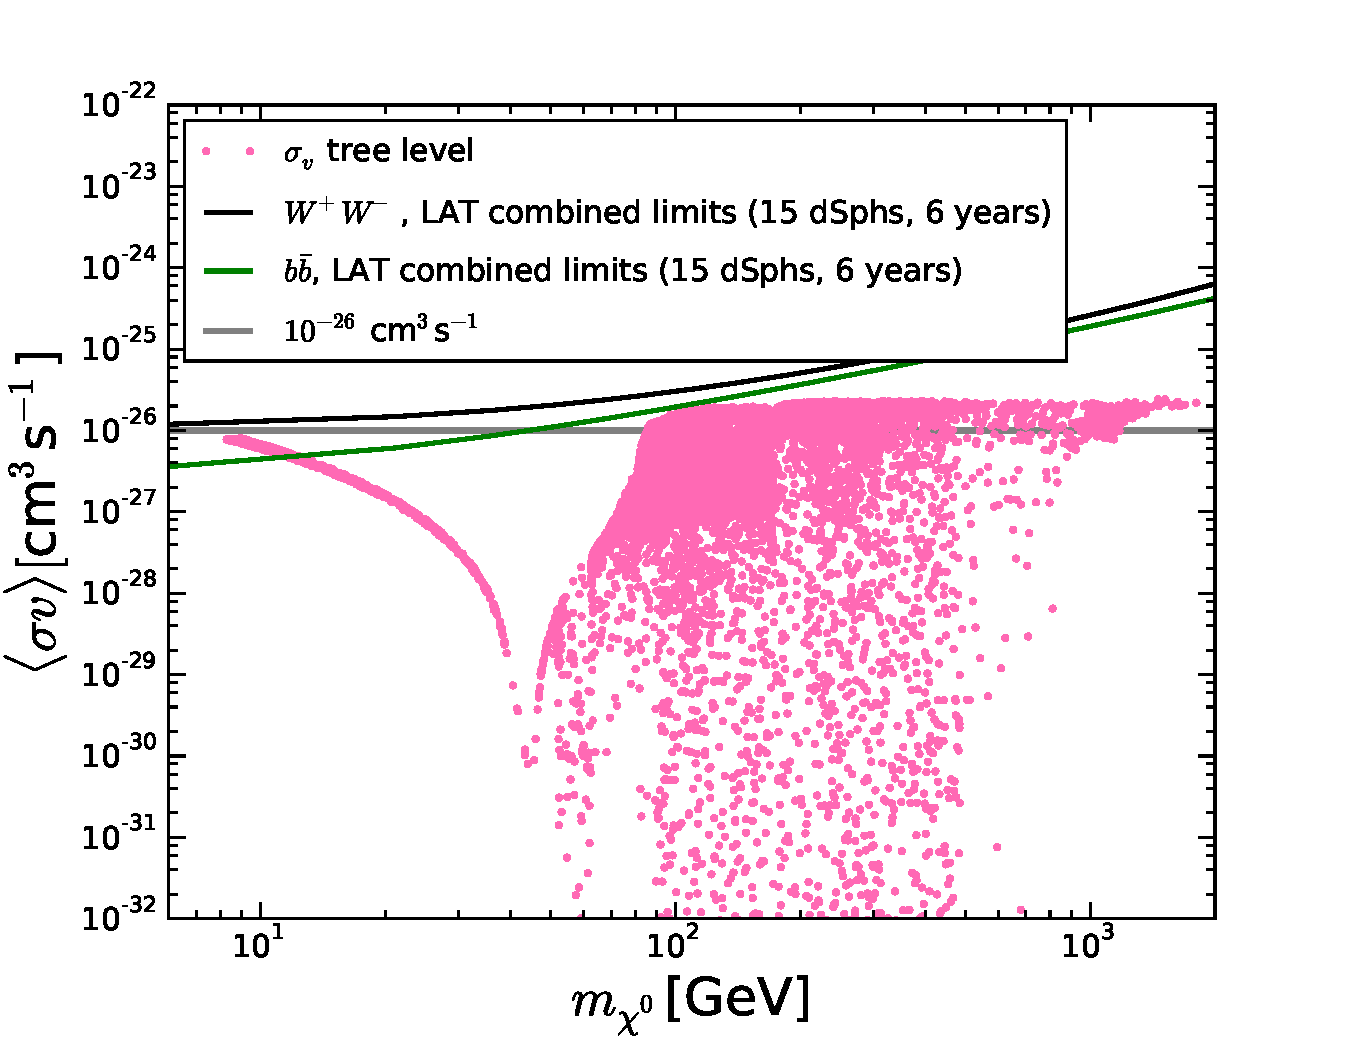
\includegraphics[scale=0.45]{sigmav-T13A}
\end{center}
\caption{Velocity average annihilation cross-section $\langle\sigma v\rangle$, generated randomly for a big sample of the parameters of the SDFDM model that take into account the correct relic density (see section~\ref{sec:Parameter-scan}). The green (black) line is the current constraint of indirect detection for DM self-annihilation into $b\bar{b}$ ($W^+W^-$) in the dwarf spheroidal galaxies (dSph) at 95$\%$ C.L~\cite{Ackermann:2015zua}. The gray line represents the prediction of the WIMP paradigm where the $\langle\sigma v\rangle$ reach the thermal value $10^{-26}\text{cm}^{3}\text{s}^{-1}$.}
\label{fig:sigmav-random}
\end{figure}
%%%%%%%%%%%%%%%%%%%%%%%%%%%%%%%%%%%%%%%%%%%%%%%%%%%%%%%%%%%%%%%%%

In Fig.~\ref{fig:sigmav-random}, it is shown the total velocity average annihilation cross-section $\langle\sigma v\rangle$ for the DM self-annihilation into SM particles including two and three final states.
%
Also, it is shown the current and strongest \textit{Fermi}  Large Area Telescope (LAT)
constraints of DM self-annihilation into $b\bar{b}$ quarks and $W^+W^-$ gauge bosons in the dwarf spheroidal galaxies (dSph). It can be seen that indirect detection does not put strong constraints on the parameter space of the SDFDM model. All the models are alive with the current indirect detection constraints.    









%%%%%%%%%%%%%%%%%%%%%%%%%%%%%%%%%%%%%%%%%%%%%%%%%%%%%%%%%%%%%%%%%%%%%
\section{Direct detection}
Regarding direct detection, the Higgs $h$ ($Z$ gauge bosson) exchanging leads to spin-independent (spin-dependent) DM nucleon scattering (see Fig.~\ref{fig:SD_SI}). From Eq.~\eqref{eq:cZXX} is clear that the spin-dependent (SD) cross section vanishes for $\cos2\beta=0$ or $|m_{\chi^0}|=M_D$, implying for both cases that $\tan\beta=\pm 1$. In the same vein, from Eq.~\eqref{eq:cHXX} the spin-independent (SI) cross section vanishes (i.e. a blind spot as discussed by Ref.~\cite{Cheung:2013dua}) for $\sin2\beta=-m_{\chi^0}/M_D$, which using the characteristic equation of the Appendix~\eqref{sec:analyt-form-mass}
leads to $m_{\chi^0}=M_N, M_D$. Note that $\sigma_{SI}=0$ if $\tan\beta<0$ and only if $M_N>M_D$, both $\sigma_{SI}$ and $\sigma_{SD}$ can be zero simultaneously. 
%
\begin{figure}[h]
  \centering
  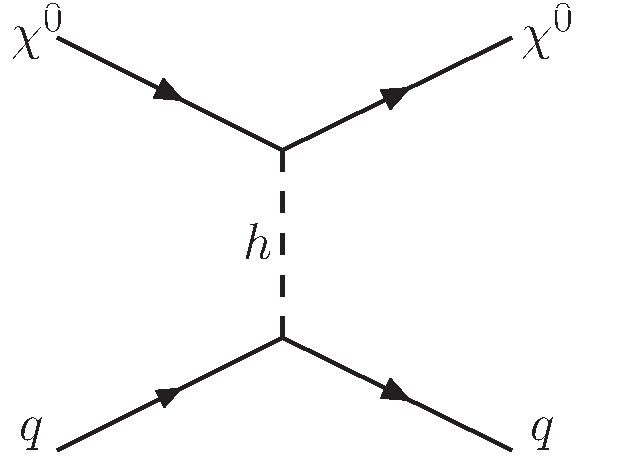
\includegraphics[scale=0.4]{SI} 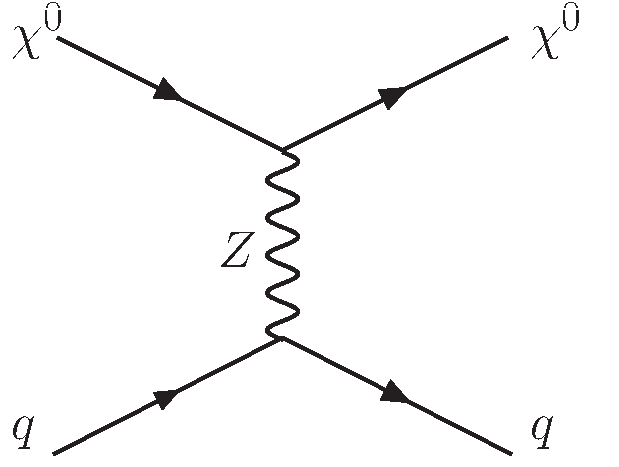
\includegraphics[scale=0.4]{SD}
  \caption{DM inelastic scattering with the quarks that compose the nucleons (protons and neutrons).}
  \label{fig:SD_SI}
\end{figure}









%%%%%%%%%%%%%%%%%%%%%%%%%%%%%%%%%%%%%%%%%%%%%%%%%%%%%%%%%%%%%%%%%%%%%%%%%%%%%%%%%%%%%%%%%%%%%%%%%%%%
\subsection{The spin-independent cross section $\sigma_{SI}$}
%
The DM scattering with the nucleons $N$ (protons and neutrons) is an effective interaction because nucleons are made of quarks. When the mediator is the Higgs gauge boson, the scalar interaction is spin-independent. In order to compute this scattering is reasonable to think in the next effective interaction
%  
\begin{align}
\mathcal{L}_{\text{SM}}\supset \sum_{q}\dfrac{m_q}{v}h\bar{q}q
= & |N\rangle\langle N|\sum_{q}\dfrac{m_q}{v}h\bar{q}q |N\rangle\langle N|
=  \dfrac{h}{v}\langle N|\sum_{q}m_q\bar{q}q|N\rangle |N\rangle\langle N| \nonumber \\
= & \dfrac{m_Nf_N}{v}h\bar{N}N\,,
\end{align}
where $\langle N|\sum_{q}m_q\bar{q}q|N\rangle=m_Nf_N$ is a QCD form factor, which is experimentally determined~\cite{Belanger:2014vza}~\cite{Abdallah:2015ter}. Using this Lagrangian, it is possible to compute the spin-independent cross section (see the Appendix~\ref{sec:SI-amplitude}). It is given by
\begin{align}
\label{eq:SI-tree-level}
\sigma_{SI}=\dfrac{m_r^2}{\pi}\left(\dfrac{c_{hX_1X_1}}{vm_h^2}\right)^2f_N^2m_N^2\,,
\end{align}
%
where $m_r=\dfrac{m_Nm_{\chi^0}}{(m_N+m_{\chi^0})}$
is the reduced mass of the dark matter-nucleon system ($m_N\approx 0.939\, \text{GeV}$ for the neutron and $m_N\approx 0.938\, \text{GeV}$ for the proton). 

%%%%%%%%%%%%%%%%%%%%%%%%%%%%%%%%%%%% PLOT: SI %%%%%%%%
\begin{figure}[h]
\begin{center}
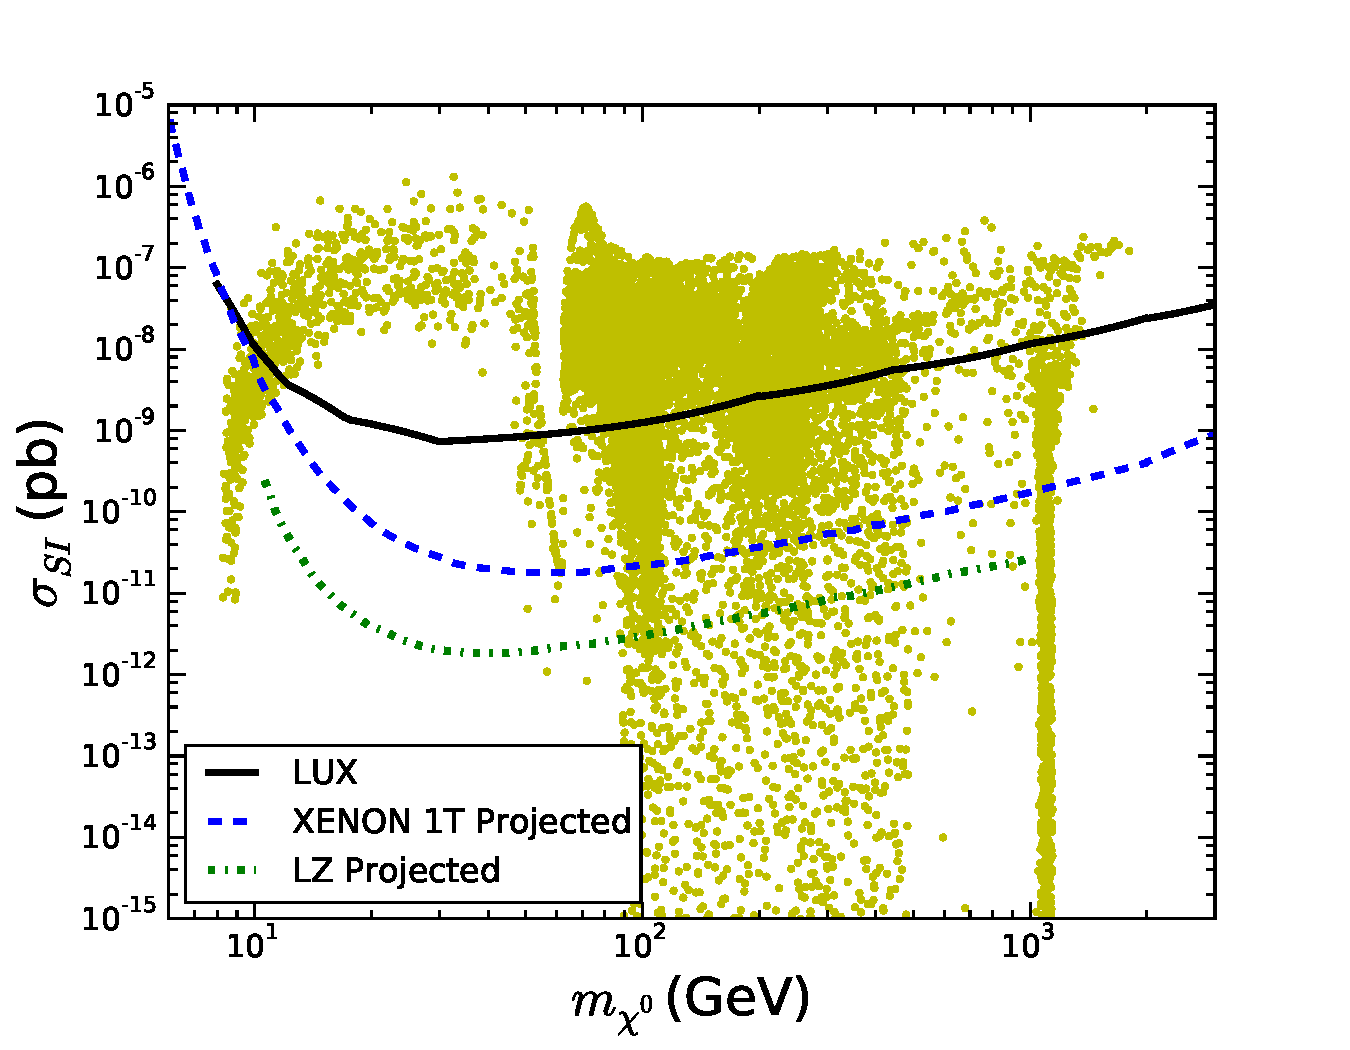
\includegraphics[scale=0.45]{sigmaSI-T13A}  
\caption{Spin-independent cross section in the SDFDM model in comparison to current and future direct detection limits. 
The panel displays current limits from the LUX experiment (black solid line)~\cite{2013arXiv1310.8214L} and the expected limits from the forthcoming XENON-1T and LZ~\cite{Cushman:2013zza} experiments (blue dashed and green dot-dashed lines).
}
\label{fig:sigma-SI}
\end{center}
\end{figure}
%%%%%%%%%%%%%%%%%%%%%%%%%%%%%%%%%%%%%%%%%%%%%%%%%%%%%%

In Fig.~\ref{fig:sigma-SI}, it is shown the spin-independent cross sections computed for a big sample of the parameters of the SDFDM model in Eq.~\eqref{eq:scan}. 
Also, it is shown the limits from the LUX-2013 experiment (black solid line)~\cite{2013arXiv1310.8214L} and the expected limits from the forthcoming XENON-1T and LZ~\cite{Cushman:2013zza} experiments (blue dashed and green dot-dashed lines).  
It can be seen that direct detection rules out some parameters space of this model. However, some of the models are alive with the current direct detection constraints.     








%%%%%%%%%%%%%%%%%%%%%%%%%%%%%%%%%%%%%%%%%%%%%%%%%%%%%%%%%%%%%%%%%%%%%%%%%%%%%%%%%%%%%%%%%%%%%%%%%%%%%%%%%%%
\subsection{The spin-dependent cross section $\sigma_{SD}$}

As it was said before, when the mediator in the scattering of the DM with nucleons $N$ (protons and neutrons) 
is the $Z$ gauge boson, the interaction is spin-dependent.
%
%%%%%%%%%%%%%%%%%%%%%%%%%%%%%%%%%%%% PLOT: SD  %%%%%%%%%%%
\begin{figure}[h]
\begin{center}
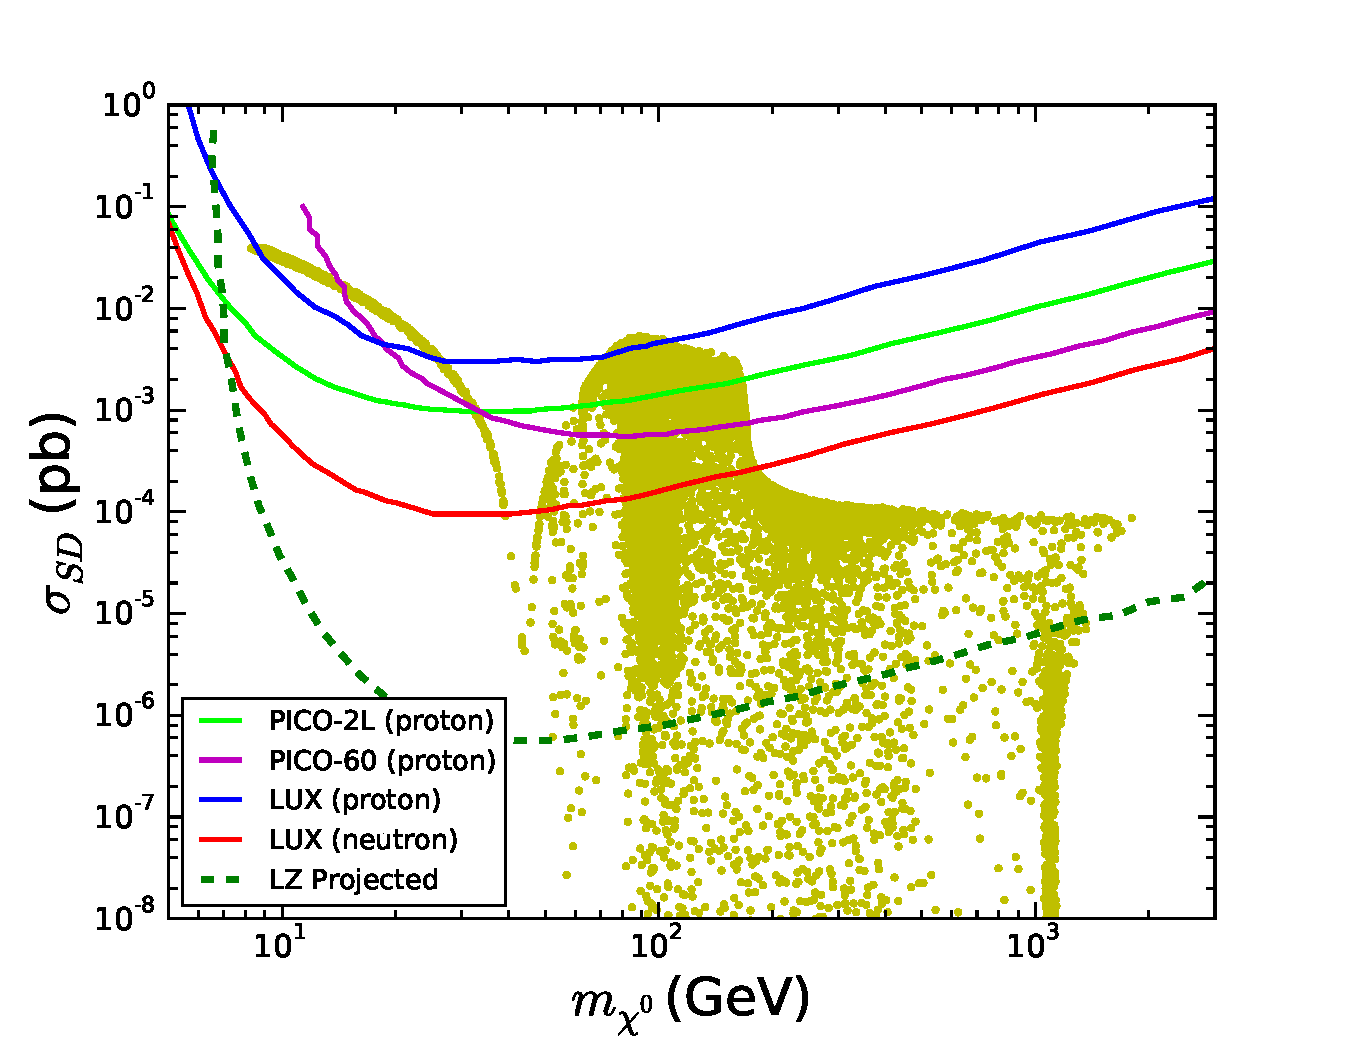
\includegraphics[scale=0.45]{sigmaSD-T13A} 
\caption{Spin-dependent cross section in the SDFDM model in comparison to current and future direct detection limits. 
The panel shows the PICO-2L~\cite{Amole:2016pye} (green light solid line) and PICO-60~\cite{Amole:2015pla} (magenta solid line) limits, as well as the LZ sensitivity (green dashed line). The most recent constraints from LUX~\cite{Akerib:2016lao} (red and blue solid lines) are also overlaid. 
}
\label{fig:sigma-SD}
\end{center}
\end{figure}
%%%%%%%%%%%%%%%%%%%%%%%%%%%%%%%%%%%%%%%%%%%%%%%%%%%%%%%%%%%%%%%
%
In Fig.~\ref{fig:sigma-SD}, it is shown the spin-dependent cross sections computed with \textsc{micrOMEGAs 4.1.8}~\cite{Belanger:2014vza} through \textsc{Feynrules 2.3}~\cite{Christensen:2008py}. Each individual model (point) saturates the Planck measurement value for the relic density $\Omega h^2=(0.1199\pm0.0027)$~\cite{Ade:2013zuv} at $3\sigma$ level. 
In Fig.~\ref{fig:sigma-SD}, it is also shown the PICO-2L~\cite{Amole:2016pye} (green light solid line) and PICO-60~\cite{Amole:2015pla} (magenta solid line) limits, as well as the LZ sensitivity (green dashed line). The most recent constraints from LUX-2016~\cite{Akerib:2016lao} (red and blue solid lines) are also overlaid. 
It can be seen that direct detection rules out some parameter space of this model. However, some of the models are alive with the current direct detection constraints, but in the future, the LZ experiment will rule out or confirm this model.

%CONECCTION
To finish this chapter, in the next section is described how to enlarge the SDFDM model in order to have masses for the active neutrinos of the SM.








%%%%%%%%%%%%%%%%%%%%%%%%%%%%%%%%%%%%%%%%%%%%%%%%%%%%%%%%%%%%%%%%%%%%%%%%%%%%%%%%%%%NEW
\section{Neutrino masses in the SDFDM model}
%
In view of the lack of signals of new physics in strong production at the
LHC, there is a growing interest in simplified models where the
production of new particles is only through electroweak processes,
with lesser constraints from LHC limits.
In particular, there are simple SM extensions with
dark matter candidates, such as the singlet scalar dark
matter (SSDM)
model~\cite{Silveira:1985rk,McDonald:1993ex,Burgess:2000yq}, or the
singlet-doublet fermion dark matter (SDFDM)
model~\cite{ArkaniHamed:2005yv,Mahbubani:2005pt,D'Eramo:2007ga,Enberg:2007rp,Cohen:2011ec,Cheung:2013dua}.
In this kind of models, the prospects for signals at LHC are in general
limited because of the softness of final SM particles coming from the
small charged to neutral mass gaps of the new particles, which is usually required 
to obtain the proper relic density.
In this sense, the addition of new particles motivated for example by
neutrino physics could open new detection possibilities, either
through new decay channels or additional mixings which increase the
mass gaps.

On those lines, scotogenic models~\cite{Ma:2006km}, featuring neutrino masses suppressed
by the same mechanism that stabilizes dark matter, have been thoroughly studied with specific predictions in almost all the current terrestrial and satellite detector experiments (For a review
see for example~\cite{Boucenna:2014zba}).
The simplest models correspond to extensions of the inert doublet
model~\cite{Deshpande:1977rw,Barbieri:2006dq} with extra singlet or
triplet fermions.
Recently, the full list of 35 scotogenic models with neutrino masses at
one-loop~\cite{Ma:1998dn,Bonnet:2012kz}~\footnote{The general
  realization of the Weinberg operator at two-loops have been undertaken
  in~\cite{Sierra:2014rxa}}, and at most triplet representations of
$SU(2)_L$, was presented in~\cite{Restrepo:2013aga} (and partially
in~\cite{Law:2013saa}).
The next to simplest scotogenic model is possibly the one where the
role of the singlet fermions is played by singlet scalars and the role
of the scalar inert doublet is played by a vector-like doublet fermion.
One additional singlet fermion is required to generate neutrino masses
at one-loop level.
This kind of extension of the singlet dark matter model is labeled
as the model T13A with $\alpha=0$ in \cite{Restrepo:2013aga}. The
extra fermion, required in order to have radiative neutrino masses, can
be the singlet in the SDFDM model.

In the simplest scotogenic model~\cite{Ma:2006km}, singlet fermion
dark matter is possible but quite restricted by lepton flavor
violation (LFV)~\cite{Toma:2013zsa,Vicente:2014wga}. 
In contrast, in the present model is shown that the region of the
parameter space, corresponding to fermion dark matter, is well below
the present and near future constraints on $\operatorname{Br}(\mu\to
e\gamma)$.

On the other hand, when the lightest $Z_2$-odd particle (LOP) is one
of the scalar singlets, in the regions of the parameter space 
compatible with constraints from LFV, the SDFDM model has promising signals at colliders,
thanks to the electroweak production of fermion doublets and possible
large branchings into charged leptons.

The dark matter phenomenology of both the SSDM and SDFDM models has
been extensively studied in the literature and recently
revisited in~\cite{Abe:2014gua}.
In this work both models will be joined and the possible effect of coannihilations with the
scalar singlets for fermion dark matter will be considered. 
We will see if these coannihilations tend to increase the relic
density of dark matter and if could modify the viable parameter space of
the SDFDM model. 








%%%%%%%%%%%%%%%%%%%%%%%%%%%%%%%%%%%%%%%%%%%%%%%%%%%%%%%%%%%%%%%%%%%%%%%%%%%%%%%%%%%%%%%%%%%%%%%%%%%%%
\subsection{The SDFDM model with reals scalars singlets}
\label{sec:model-with-scalars}
%
When the SDFDM model is extended with a set of 
real scalar singlets  $S_{\alpha}$ of zero hypercharge
and odd under the imposed $Z_2$ symmetry,
the most general $Z_2$-invariant Lagrangian is given by
\begin{align}
\label{eq:lt13a}
 \mathcal{L}= &\mathcal{L}_{\text{SM}}+ M_D \epsilon_{ab}R^a_d \widetilde{R}^b_u-\tfrac{1}{2}M_N NN-h_{i\alpha} \epsilon_{ab}\widetilde{R}_u^a L_{i}^b S_{\alpha}-\lambda_d\, \epsilon_{ab}H^a R_d^b N-\lambda_u \epsilon_{ab}\widetilde{H}^a \widetilde{R}_u^b N+\text{h.c}\nonumber\\
&-\left[ 
\tfrac{1}{2}\left({M}_S^2\right)_{\alpha\beta} S_{\alpha}S_\beta
   +\lambda^{SH}_{\alpha\beta} \epsilon_{ab}\widetilde{H}^{a}H^bS_{\alpha}S_{\beta}+\lambda^{S}_{\alpha\beta\gamma\delta}S_{\alpha}S_{\beta}S_{\gamma}S_{\delta} 
\right], 
\end{align}
where $L_{i}$ are the lepton doublets and $H$ is the SM Higgs.

In the scalar potential, it is assumed that the $M_{S}^{2}$ matrix has only
positive entries and $\left(M_S^2 \right)_{\alpha\beta}+\lambda^{SH}_{\alpha\beta}v^2=0$ for $\alpha\ne\beta$,  which means that $S_\alpha$ are mass eigenstates with masses $m_{S_{\alpha}}^{2}=\left({M}_S^2 \right)_{\alpha\alpha}+\lambda^{SH}_{\alpha\alpha}v^2$ and $m_{S_\alpha}<m_{S_{\alpha+1}}$.
%







%%%%%%%%%%%%%%%%%%%%%%%%%%%%%%%%%%%%%%%%%%%%%%%%%%%%%%%%%%%%
\subsection{One-loop neutrino masses}
\label{sec:one-loop masees}
%
In this framework, the new fields $N,\widetilde{R}_u,R_d,S$ do not carry lepton number so that the
only lepton-number violating terms is the one with coupling $h_{i\alpha}$. 
The radiative neutrino mass matrix is obtained 
using the realization of the Weinberg operator a one-loop {\color{blue} how it was pointed out in Fig.[5] of the Ref.~\cite{Ma:1998dn} and as one of the topology T1-iii in~\cite{Bonnet:2012kz}}. 
The computation of the neutrino mass matrix can be done in the interaction basis as it is shown on the Appendix~\ref{sec:mass-interaction-basis}.
However, it is more illustrative to show the calculation on the basis of mass eigenstates as follows.

After the EWSB, each entry of the neutrino mass matrix have the three fermion contributions ($n=1,2,3$) displayed in Fig.~\ref{fig:T13Aweylme}, each one with divergent parts which must cancel between them.  
\begin{figure}
  \centering
  %\includegraphics[scale=0.25]{T13Aweylme1} \includegraphics[scale=0.25]{T13Aweylme2} \includegraphics[scale=0.25]{T13Aweylme3}
  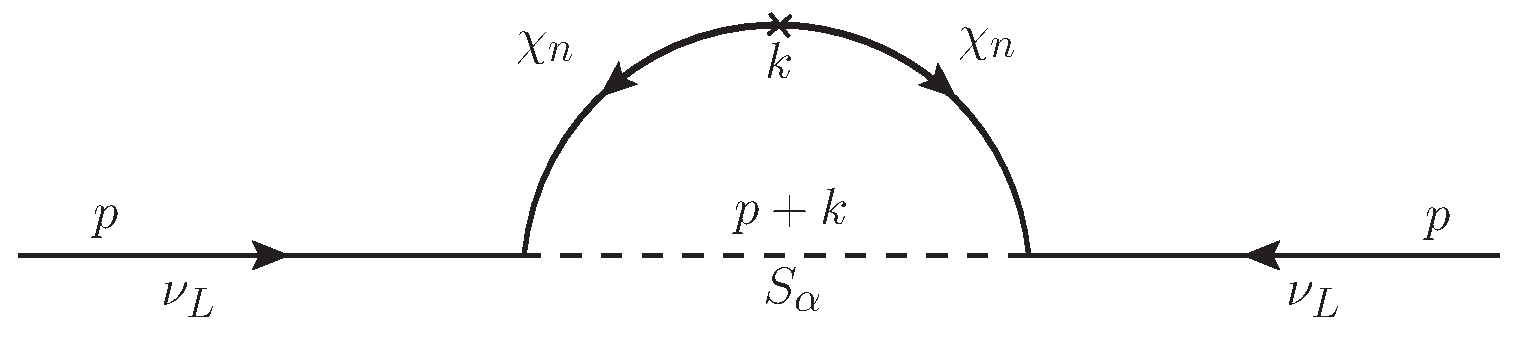
\includegraphics[scale=0.4]{neutrino_mass_diagram}
  \caption{Contributions to the neutrino mass matrix.}
  \label{fig:T13Aweylme}
\end{figure}
%
The neutrino mass matrix in this basis is given by
\begin{align*}
  M^{\nu}_{ij}=&i\sum_{\alpha}\int \frac{d^4k}{(2\pi)^4}\sum_{n=1}^3 \left( -i h_{i\alpha} N_{3n} \right) i S_F(k)\left( -i h_{j\alpha} N_{3n} \right)i\Delta_F(p+k)\nonumber\\
=&i\sum_{\alpha}\frac{h_{i\alpha}h_{j\alpha}}{16\pi^2}\sum_{n=1}^3 \left( N_{3n} \right)^2\int \frac{d^4k}{\pi^2}\frac{\cancel{k}+m_{\chi_n}}{\left(k^2-m_{\chi_n}^2  \right)\left[\left(p+k\right)^2-m_{S_\alpha}^2\right]}\,.
\end{align*}
In the limit of $p\to 0$, we have
\begin{align}
\label{eq:mnueig}
  M^{\nu}_{ij}=&i^2\sum_{\alpha}\frac{h_{i\alpha}h_{j\alpha}}{16\pi^2}\sum_{n=1}^3 \left( N_{3n} \right)^2m_{\chi_n}\; B_0 \left(0;m_{\chi_n}^2,m^2_{S_{\alpha}} \right)\,,
\end{align}
where $B_0$ is the Passarino Veltman functions given by~\cite{Passarino:1978jh}
%
\begin{align}
B_0 \left(0;m_{\chi_n}^2,m^2_{S_{\alpha}} \right)=&\int \frac{d^4k}{i\pi^2}\frac{1}{\left(k^2-m_{\chi_n}^2\right)\left(k^2-m_{S_\alpha}^2\right)}
=\frac{1}{m_{\chi_n}^2-m_{S_\alpha}^2}\left[ A_0\left(m_{\chi_n}^2\right)-A_0\left(m_{S_\alpha}^2\right)  \right] 
\end{align}
%
with
\begin{align}
A_0\left(m^2\right)=&\, m^2 \left[ \left( \frac{2}{\epsilon}-\ln\pi+\gamma_E \right)+1-\ln \left(\dfrac{m^2}{\mu^2} \right) \right] \,.
\end{align}

In order to compute this matrix, two things need to be used. 
First, the Eq.~\eqref{eq:mnueig}, where 
\begin{align}
\label{eq:mnueigdev}
\sum_{n=1}^3& \left( N_{3n} \right)^2m_{\chi_n}\; B_0 \left(0;m_{\chi_n}^2,m^2_{S_\alpha} \right)\nonumber\\
  &=\sum_{n=1}^3 \left( N_{3n} \right)^2m_{\chi_n}
   \left\{\frac{1}{m_{\chi_n}^2-m_{S_\alpha}^2}\left[m^2_{\chi_n} \left[ \Delta+1-\ln \left( m_{\chi_n}^2/\mu^2 \right) \right]   
-m_{S_\alpha}^2 \left[ \Delta+1-\ln \left( m_{S_\alpha}^2/\mu^2 \right) \right]\right] \right\}\nonumber\\
&=\sum_{n=1}^3 \left( N_{3n} \right)^2m_{\chi_n}
   \left\{(\Delta+1)+\frac{m_{S_\alpha}^2\ln \left( m_{S_\alpha}^2/\mu^2 \right)-m_{\chi_n}^2\ln \left( m_{\chi_n}^2/\mu^2 \right)}{m_{\chi_n}^2-m_{S_\alpha}^2} \right\}\nonumber\\
&=\sum_{n=1}^3 \left( N_{3n} \right)^2m_{\chi_n}
   \left\{\left[\Delta+1+\ln\left( \mu^2 \right) \right]+\frac{m_{S_\alpha}^2\ln \left( m_{S_\alpha}^2 \right)-m_{\chi_n}^2\ln \left( m_{\chi_n}^2 \right)}{m_{\chi_n}^2-m_{S_\alpha}^2} \right\}\,,
\end{align}
%
and second, the Eq.~\eqref{eq:chidiag}, where
%
\begin{align}
\label{eq:divcan}
\mathbf{N} \mathbf{M}^\chi_{\text{diag}}\mathbf{N}^{\operatorname{T}}=\mathbf{M}^\chi\Rightarrow \sum_mN_{lm}m_{\chi_m} N_{nm}=(M^\chi)_{ln}\,, \Rightarrow
  \sum_m N_{3m}^2m_{\chi_m}=(M^\chi)_{33}=0\,.
\end{align}
%
%The explicit expression for $\mathbf{M}^{\chi}$ was used for $l=n=3\,$~\eqref{eq:Mchi}.
 
Finally, using the Eq.~\eqref{eq:mnueigdev} and Eq.~\eqref{eq:divcan} the neutrino mass matrix takes the form
%
\begin{align}
\label{eq:neutrino-mass-matrix}
M^{\nu}_{ij}=&\sum_{\alpha}\frac{h_{i\alpha}h_{j\alpha}}{16\pi^2}\sum_{n=1}^3 \left( N_{3n} \right)^2m_{\chi_n}
\left[ \frac{m_{\chi_n}^2\ln \left( m_{\chi_n}^2 \right)-m_{S_\alpha}^2\ln \left( m_{S_\alpha}^2 \right)}{m_{\chi_n}^2-m_{S_\alpha}^2} \right]\,.
\end{align}







%
\chapter{Phenomenology of the SDFDM model with real scalars singlets}

\begin{flushright}
This chapter in based in our work published in \textbf{PhysRevD.92.013005 (2015)}\\ 
\url{http://dx.doi.org/10.1103/PhysRevD.92.013005}
\end{flushright}
\begin{center}
\textbf{Abstract}
\end{center}

  \InitialCharacter{W}hen the singlet-doublet fermion dark matter model is extended with
  additional $Z_2$--odd real  singlet scalars, neutrino masses and mixings
  can be generated at one-loop level.  In this work, we discuss the salient 
  features arising from the combination of the two resulting
  simplified dark matter models.  When the $Z_2$-lightest odd particle is a
  scalar singlet, $\operatorname{Br}(\mu\to e \gamma)$ could be
  measurable provided that the singlet-doublet fermion mixing is small
  enough. In this scenario, also the new decay channels of vector-like
  fermions into scalars can generate interesting leptonic plus
  missing transverse energy signals at the LHC. On the other hand, in
  the case of doublet-like fermion dark matter, scalar coannihilations
  lead to an increase in the relic density which allows to lower the bound of
  doublet-like fermion dark matter.








%%%%%%%%%%%%%%%%%%%%%%%%%%%%%%%%%%%%%%
\section{Neutrino masses}

When we extended the SDFDM model with real scalars singlets we were able to get neutrino masses using the realization of the Weinberg operator as it was described in the section~\ref{sec:one-loop masees}.  
In general, is possible to write the neutrino mass matrix~\eqref{eq:neutrino-mass-matrix} as
%
\begin{align}
   M^{\nu}_{ij}=&\sum_{\alpha}\frac{h_{i\alpha}h_{j\alpha}}{16\pi^2}\sum_{n=1}^3 \left( N_{3n} \right)^2m_{\chi_n}
\,f\left( m_{S_\alpha},m_{\chi_n} \right) ,\\\label{eq:Mnuij}
=&\sum_{\alpha} h_{i\alpha} \Lambda_{\alpha} h_{j\alpha}\\\label{eq:CI}
=&\left( \mathbf{h}\mathbf{\Lambda}\mathbf{h}^{\operatorname{T}} \right)_{ij}\,,
\end{align}
with
$f \left( m_1,m_2 \right)= (m_1^2\,\ln  m_1^2 -m_2^2\,\ln m_2^2 )/(m_1^2-m_2^2)$, $\boldsymbol{\Lambda}=\operatorname{Diag}\left(\Lambda_1,\Lambda_2,\Lambda_3\right)$ and
\begin{align}
\label{eq:Lambda}
  \Lambda_\alpha=&\frac{1}{16\pi^2}\sum_{n=1}^3 \left( N_{3n} \right)^2m_{\chi_n}\,f\left( m_{S_\alpha},m_{\chi_n} \right)\,.
\end{align}

As we described in the Appendix~\ref{sec:casas-ibarra}, the flavor structure of the neutrino mass matrix $M^{\nu}_{ij}$, given
by Eq.~\eqref{eq:CI}, allows us to express the Yukawa couplings in
terms of the neutrino oscillation observables (ensuring the proper
compatibility with them) through the Casas-Ibarra parametrization introduced in
\cite{Casas:2001sr,Ibarra:2003up}. 
Thus, by using an arbitrary complex orthogonal rotation matrix
$\boldsymbol{\mathcal{R}}$, the Yukawa couplings $h_{i\alpha}$ are
given by
\begin{align}
  \label{eq:ht}
  \mathbf{h}^{T}=\mathbf{D}_{\sqrt{{\Lambda}^{-1}}}\,\boldsymbol{\mathcal{R}}\,\mathbf{D}_{\sqrt{m_{\nu}}}\,\mathbf{U}^{\dagger} \,,
\end{align}
where $\mathbf{D}_{\sqrt{m_\nu}}=\operatorname{Diag}
\left(\sqrt{m_{\nu 1}} , \sqrt{m_{\nu2}},\sqrt{m_{\nu3}}\right)$,
$\mathbf{D}_{\sqrt{\Lambda^{-1}}}=\operatorname{Diag}
\left(\sqrt{\Lambda_1^{-1}} , \sqrt{\Lambda_2^{-1}},\cdots\right)$ and
$\mathbf{U}$ is the PMNS~\cite{Maki:1962mu} neutrino mixing matrix.

Henceforth, we will consider the case of three scalar singlets, $\alpha=1,2,3$,
where the Yukawa couplings take the form
\begin{align}
\label{eq:Y_CIww}
 h_{i\alpha}=&\frac{\sqrt{m_{\nu 1}}{\mathcal{R}}_{\alpha 1}U_{i1}^*+\sqrt{m_{\nu 2}}{\mathcal{R}}_{\alpha 2} U^{*}_{i2}+ \sqrt{m_{\nu 3}}{\mathcal{R}}_{\alpha 3} U^{*}_{i3}}{\sqrt{\Lambda_\alpha}}\,.
\end{align}
In the above equation, the $3\times3$ matrix
$\boldsymbol{\mathcal{R}}$ can be cast in terms of three rotation
angles $\theta_{23},\theta_{13},\theta_{12}$, which are assumed to be real. 
It is worth mentioning that for the case two scalar singlets
$\alpha=1,2$ a viable scenario is also possible with the remarks that
one massless neutrino is obtained. 
To fully exploit the generality of $h_{i\alpha}$ couplings obtained
from~\eqref{eq:Y_CIww}, we stick to the case with three scalar singlets.

In summary, the set of input parameters of the model are the scalar masses
$m_{S_\alpha}$, $M_N$, $M_D$, $\lambda$,
$\tan\beta$, the lightest neutrino mass $m_{\nu1}$, the three rotation 
angles present in $\boldsymbol{\mathcal{R}}$  
and $\lambda^{SH}_{\alpha\beta}$\footnote{The couplings $\lambda^{S}_{\alpha\beta\gamma\delta}$ are irrelevant for phenomenological purposes.}. Without not loss of generality we assume for the latter to be small $\lambda^{SH}_{\alpha\beta}\lesssim0.01$, except for the case of scalar dark matter where $\lambda^{SH}_{11}$ is set to give 
the proper relic density.

In order to have an approximate expression for $\Lambda_\alpha$ in terms of this set of input parameters, it is possible to use the identity~(\ref{eq:divcan}) to obtain
\begin{align*}
\Lambda_\alpha=&\frac{1}{16\pi^2}\left\{N_{31}^2\,m^\chi_1\left[ f(m_{S_\alpha},m^\chi_1)-f(m_{S_\alpha},m^\chi_3)\right]
                                +N_{32}^2\,m^\chi_2\left[f(m_{S_\alpha},m^\chi_2)-f(m_{S_\alpha},m^\chi_3)\right]\right\}\,.
\end{align*}
The expression for the matrix elements $N_{31}^2$ at $\mathcal{O}\left( m_{\lambda}^2 \right)$ are given in the Appendix~\ref{sec:analyt-form-mass}. Since $N_{31}^2$ and $f(m_{S_\alpha},m^\chi_2)-f(m_{S_\alpha},m^\chi_3)$ are already $\mathcal{O}\left( m_{\lambda}^2 \right)$, we can use the leading order values for the other masses and mixings parameters to obtain
\begin{align*}
  \Lambda_\alpha\approx&\frac{1}{16\pi^2}\left\{N_{31}^2 M_N\left[ f(m_{S_\alpha},M_N)-f(m_{S_\alpha},M_D)\right]
                                +\frac{1}{2}M_D\left[f(m_{S_\alpha},m^\chi_2)-f(m_{S_\alpha},m^\chi_3)\right]\right\}
+\mathcal{O}\left( m_\lambda^4 \right)\,.
\end{align*}
With the last two approximate formula for masses in \eqref{eq:ml2},  and the $N_{31}^2$  mixing in~\eqref{eq:mixl2}, we have
\begin{align}
\label{eq:lambdaappr}
16\pi^2\frac{\Lambda_\alpha}{m_{\lambda}^{2}}\approx & \left(\frac{M_{D} \cos\beta + M_{N} \sin\beta}{M_{D}^{2} - M_{N}^{2}}\right)^{2}
                                  M_{N}\left[f(m_{S_\alpha},M_N)-f(m_{S_\alpha},M_D)\right]\nonumber\\
&+\frac{ M_{D}^{2}\left[M_{D} \sin\left(2 \beta \right ) + M_{N}\right] 
        }{\left(M_{D}^{2} - M_{N}^{2}\right) \left(M_{D}^{2} - m_{S_\alpha}^{2}\right)^{2}} \left\{M_{D}^{2} - m_{S_\alpha}^{2} \left[\log{\left (\frac{M_{D}^{2}}{m_{S_\alpha}^{2}} \right )} + 1\right]\right\}+\mathcal{O}\left( m_\lambda^2 \right)\,.
\end{align}
%
To illustrate the dependence in $\tan\beta$ of $\Lambda_{\alpha}$, we consider the following set of input masses (SIM) compatible with singlet scalar dark matter:
\begin{align}
\label{eq:bp}
  m_{S_1}&=\SI{60}{GeV} & m_{S_2}=&\SI{800}{GeV} & m_{S_3}=&\SI{1500}{GeV}\, \nonumber\\
  m_N&=\SI{100}{GeV} & m_D=&\SI{550}{GeV}\,.
\end{align}
The results for $\lambda=\num{5E-3}$ are shown in
Fig.~\ref{fig:Lambdaa}(a). For large values of $\tan\beta$, the
$\Lambda_{\alpha}$ are positive. However, there are specific values of $\tan\beta$ for which each $\Lambda_{\alpha}$ 
goes to zero and turns to negative values, as illustrated by the red lines in the plot. 
The specific point with $\beta=\pi/6$ is depicted by the yellow stars in the figure.

\begin{figure}
\centering
(a) \hfill (b)\\
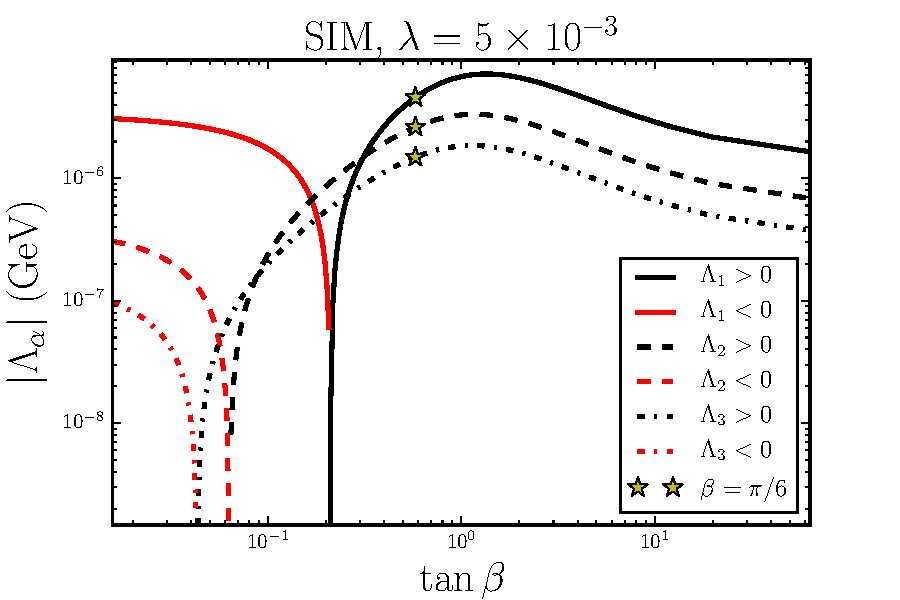
\includegraphics[scale=0.55]{tanbdependence}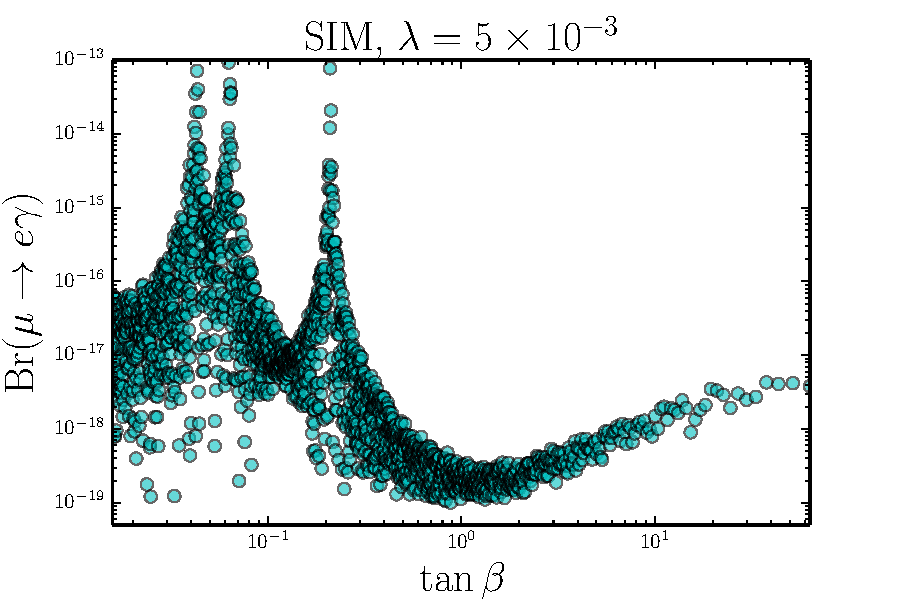
\includegraphics[scale=0.55]{brmuegammatanb}
\caption{$\tan\beta$ dependence of (a) $\Lambda_a$ and (b) $\operatorname{Br}(\mu \rightarrow e \gamma)$, for the set of input masses in Eq.~\eqref{eq:bp} with
$\lambda=\num{5E-3}$.}
\label{fig:Lambdaa}
\end{figure}









%%%%%%%%%%%%%%%%%%%%%%%%%%%%%%%%%%%%%%%%%%%%%%%%%%%%%%%%%%%%%%%%%%%%%%%%%%%%%%%%%%%%%%%%%%%%%%%%%%%%
\section{Lepton flavor violation}
\label{sec:lept-flav-viol}

The size of the lepton flavor violation (LFV) is controlled by the lepton
number violating couplings $h_{i\alpha}$.  
From the approximate expression for $\Lambda_{\alpha}$ found in the Eq.~\eqref{eq:lambdaappr} and the analysis of the previous section, we
will show that these couplings are inversely related to the Yukawa
coupling strength $\lambda$.
Since in SDFDM the observed dark matter abundance is typically
obtained for $\lambda\gtrsim 0.1$~\cite{Cheung:2013dua}, the lepton
flavor observables are not expected to give better constraints than
the obtained from direct detection experiments. Therefore, we will
focus our discussion of LFV in regions of the parameter space
where $S_1$ is the dark matter candidate.

\begin{figure}[h]
\centering
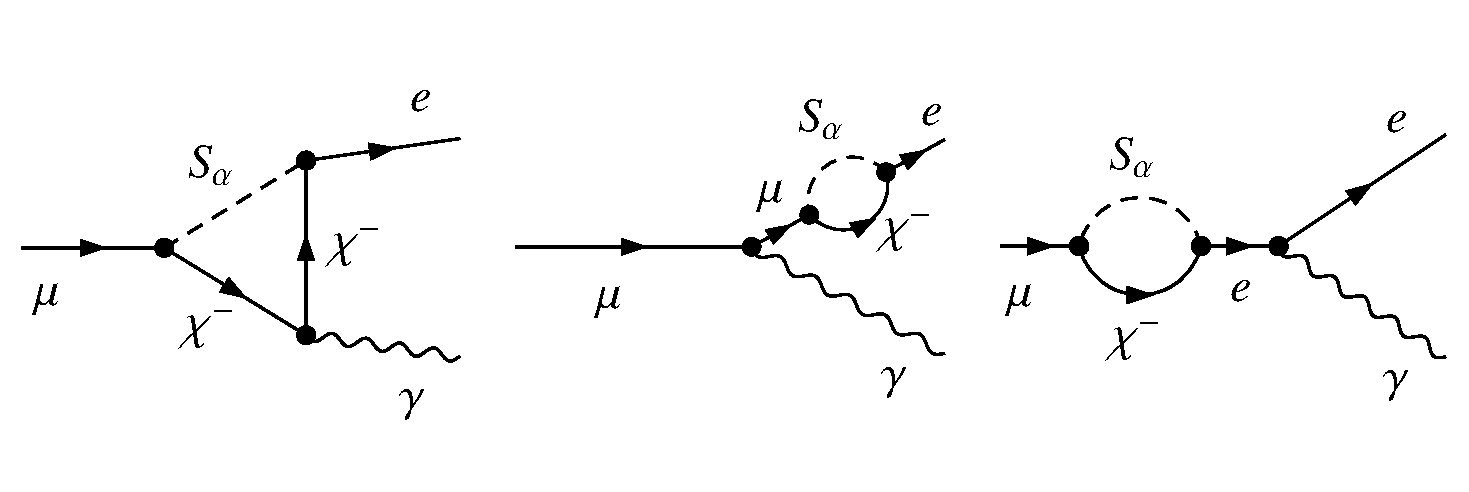
\includegraphics[scale=0.5]{t13a-muegamma1}
\caption{$\mu \to e \gamma$ process generated using \textsc{FeynArts}~\cite{Hahn:2000kx}.}
\label{fig:muegamma}
\end{figure}

It is well known that LFV processes put severe constraints on the LFV
couplings and, in general, on the model's parameter space. 
One of the most restrictive LFV processes is the radiative muon decay
$\mu\to e\gamma$ shown in Fig.~\ref{fig:muegamma}, which in the present model is mediated by same
particles present in the internal lines of the one-loop neutrino mass
diagram shown in Fig.~\ref{fig:T13Aweylme}. 
The corresponding expression for the branching ratio is computed in the Appendix~\ref{sec:Ap-muegamma}. It is given by
%
\begin{align}
\label{eq:muegamma}
\operatorname{Br}(\mu \rightarrow e \gamma)=&\dfrac{3}{4}\dfrac{\alpha_{\text{em}}}{16 \pi G_F^2}\left|\sum_{\alpha}
h_{1\alpha}\frac{F\left(M_D^2/m_{S_{\alpha}}^2  \right) }{m_{S_\alpha}^2}h_{2\alpha}^{*}  \right|^2 ,
\end{align}
where
\begin{align}
F(x)=\dfrac{x^3-6x^2+3x+2+6x\ln x}{6(x-1)^4}\,.
\end{align}
%
With the implementation of the model in the
\texttt{BSM-Toolbox}~\cite{Staub:2011dp} of
\texttt{SARAH}~\cite{Staub:2008uz,Staub:2013tta}, we have crosschecked
the one-loop results for both neutrino masses and $\operatorname{Br}(\mu
\rightarrow e \gamma)$.
Moreover, with the \texttt{SARAH}
\texttt{FlavorKit}~\cite{Porod:2014xia}, we have also checked that the
most restrictive lepton flavor violating process in the scan is just Br($\mu\to e\gamma$).
%
From Eqs.~\eqref{eq:Mnuij} and~\eqref{eq:ht}, we obtain
\begin{align}
  M^{\nu}_{12}=\sum_{\alpha} h_{1\alpha} \Lambda_{\alpha}
  h_{2\alpha}=\left[ \mathbf{U}^{*}\mathbf{M}^{\nu}_{\text{diag}}\mathbf{U}^{\dagger} \right]_{12}\,.%=\sum_{j}m_{\nu j}U_{1j}^{*}U_{2j}^{*}\,.
\end{align}
Comparing this result with the corresponding combination of couplings
in the expression for Br$(\mu\to e\gamma)$ in Eq.~\eqref{eq:muegamma},
we expect that for a set of fixed input masses $\operatorname{Br}(\mu
\rightarrow e \gamma)$ turns out to be inversely proportional to
$\Lambda_\alpha^2$.
This is illustrated in Fig.~\ref{fig:Lambdaa}(b)
for $\lambda=\num{5E-3}$, where the scatter plot of
$\operatorname{Br}(\mu\to e \gamma)$ is shown for the same range of $\tan\beta$ values 
 than in Fig.~\ref{fig:Lambdaa}(a).  In such a case, once
$h_{i\alpha}$ are obtained from the Casas-Ibarra parametrization, the
specific hierarchy of $\Lambda_{\alpha}$ fixes the several contributions
to $\operatorname{Br}(\mu \rightarrow e \gamma)$.  The dispersion of
the points is due to the 3-$\sigma$ variation of neutrino oscillation
data~\cite{Forero:2014bxa} used in the numerical implementation of the Casas-Ibarra
 parametrization, along with the random variation of the parameters of
$\boldsymbol{\mathcal{R}}$. The minimum value of
$\operatorname{Br}(\mu \rightarrow e \gamma)$ around $\tan\beta=1$
corresponds to the maximum value of $\Lambda_{\alpha}$, while the
maximum values happen at the cancellation points of each
$\Lambda_{\alpha}$. In the subsequent analysis, and for a fixed SIM and $\lambda$, we allow 
for cancellations only by two orders of magnitude from the maximum
value of each $\Lambda_{\alpha}$. 

The full scan of the input masses up to $\SI{2}{TeV}$, with
$m_{S_1}>\SI{53}{GeV}$~\cite{Abe:2014gua} as the dark matter candidate,
$M_D>\SI{100}{GeV}$ to satisfy LEP constraints, and
$10^{-2}\le\tan\beta\le 10^2$, give to arise the dark-gray plus
light-gray regions in Fig.~\ref{fig:brmuegamma}. In particular, the
$\lambda$ variation for the SIM with $\beta=\pi/6$, denoted by yellow
stars in Fig.~\ref{fig:Lambdaa}(a), is illustrated
with the white dots in Fig.~\ref{fig:brmuegamma}.   The
corresponding dashed line is obtained for the best-fit values of the
neutrino oscillation data and $\boldsymbol{\mathcal{R}}$ fixed to the
identity. The horizontal dotted line in the plot corresponds to the
current experimental bound for $\operatorname{Br}(\mu\to e
\gamma)<\num{5.7E-13}$ at $90\%\,\si{CL}$~\cite{Adam:2013mnn}.  
The upper part of the 
light-gray region is restricted by our imposition to avoid too strong
cancellation in  $\Lambda_{\alpha}$ . We check that for all the sets of
input masses in the random scan, this cancellation region always
happens when $\tan\beta<1$. In this way, points with $\tan\beta>1$ are
absent from the light-gray region, as labeled in
Fig.~\ref{fig:brmuegamma}. For the same reason, in the dark-gray
region there are not points with $\Lambda_{\alpha}\ll
\Lambda_{\beta}\sim \Lambda_\gamma$ ($\alpha\ne\beta\ne\gamma$). We can check for example that
points with $\Lambda_1\ll \Lambda_2<\Lambda_3$ are absent inside the
dark-gray region of Fig.~\ref{fig:brmuegamma}.


\begin{figure}
  \centering
  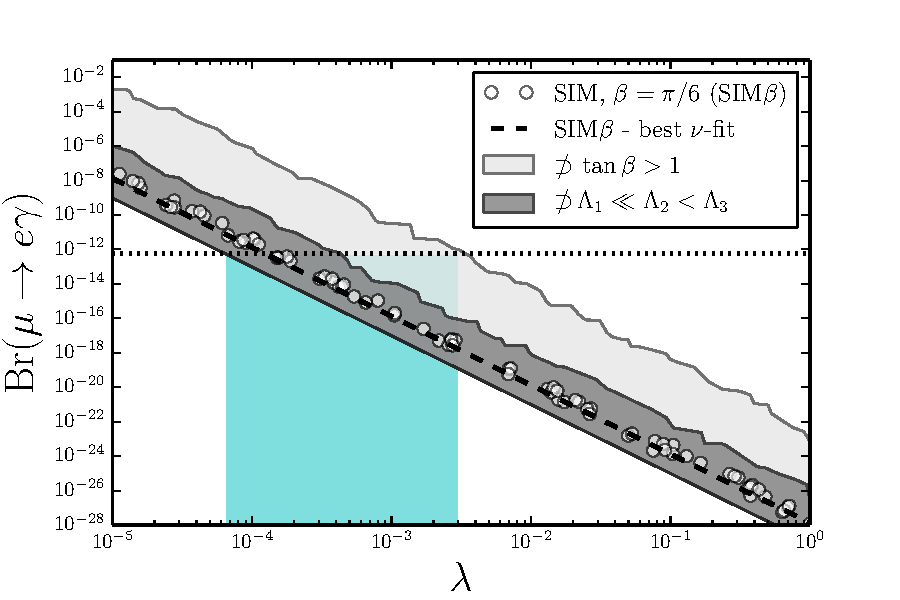
\includegraphics[scale=0.7]{brmuegamma}
  \caption{$\operatorname{Br}(\mu \rightarrow e \gamma)$ in terms of
    the Yukawa coupling strength $\lambda$ for the SIM in
    Eq.~\eqref{eq:bp} with $\beta=\pi/6$, and the general scan
    described in the text.}
  \label{fig:brmuegamma}
\end{figure}



The lower part of the dark-gray region is saturated by the values of
$M_{D}=\SI{2}{TeV}$, and gives rise to the lower bound $\lambda\gtrsim
\num{6E-5}$. 
With our restriction in the cancellation of
$\Lambda_{\alpha}$,  points in the scan with $\lambda\lesssim\num{3E-3}$ 
can be excluded from the Br$(\mu\to e\gamma)$ limit.    









%%%%%%%%%%%%%%%%%%%%%%%%%%%%%%%%%%%%%%%%%%%%%%%%%%%%%%%%%%%%%%%%%%%%%%%%%%%%%%%%%%%%%%%%%%%%%%%%%%%%
\section{Collider phenomenology}
\label{sec:collider-phenomenology}

The LHC phenomenology in the case of the singlet-doublet fermion
dark matter was already analyzed in~\cite{Abe:2014gua}. They concluded that
the recast of the current LHC data is easier to evade, but the
long-run prospects are promising, since the region $M_N,m_\lambda\ll M_D$ could be 
probed up to $M_D\lesssim 600-\SI{700}{GeV}$ for the 14-TeV run of the LHC with 
$\SI{3000}{fb}^{-1}$. 

On the other hand, in the case of the singlet scalar dark matter, the
main production processes associated with the new fermions remain the
same, but there are new signals from the mediation, or presence in the
final decay chains, of the new scalars.
The most promising possibility is the dilepton plus missing
transverse energy signal coming from the production of
charged fermions decaying into leptons and the lightest scalar.
This signal can be important when $\lambda$ is
not too large, $\lambda\lesssim 0.1$, and $M_N\gtrsim M_D$. 
For a fixed set of input parameters, the random phases in the
Casas-Ibarra can be chosen to have all the possibilities in the lepton
flavor space associated with the coupling $h_{i1}$, with
$i=e,\mu,\tau$. 
In view of that, we will focus in the best scenario where
$\operatorname{Br}(\chi^\pm\to l^\pm \, S_1 )\approx 1$ ($l^\pm=e^\pm$ or
$\mu^\pm$). 
The Feynman diagram for the processes is displayed in
Fig.~\ref{fig:chain_signal}.

   
The mass of the  charged  Dirac fermion $\chi^{\pm}$, can be
constrained from dilepton plus missing transverse energy  searches at the  LHC.
In~\cite{Aad:2014vma}, this kind of signals was used by the ATLAS
collaboration to establish bounds on the slepton masses from the
search for $pp \rightarrow \tilde{l}^+\tilde{l}^- \rightarrow l^+l^-
\tilde{\chi}^0\tilde{\chi}^0$, where $\tilde{\chi}^{0}$ are the neutralinos,
and the same exclusion is reported for $l=e$ or $\mu$.
Purely left-handed sleptons produced and decaying this way, have been
excluded up to masses of about $300$ GeV at 95\% CL, from the data
with integrated luminosity of 20.3 fb$^{-1}$ and the $pp$ collision
energy of 8 TeV. 
This corresponds to an excluded cross section of $\SI{1.4}{fb}$ at NLO
calculated with \texttt{PROSPINO}~\cite{Beenakker:1996ed}.

In the present model, the charged fermion field may decay in the
mode $\chi^{\pm} \rightarrow e_i^{\pm}S_1$ which are
proportional to the Yukawa couplings $h_{i1}$. 
Therefore, a similar final state as in the slepton pair production is
obtained through the process $pp \rightarrow \chi^+\chi^- \rightarrow
l^+l^- S_1 S_1$, as can be seen in Fig.~\ref{fig:chain_signal}.


\begin{figure}[h]
\begin{center}
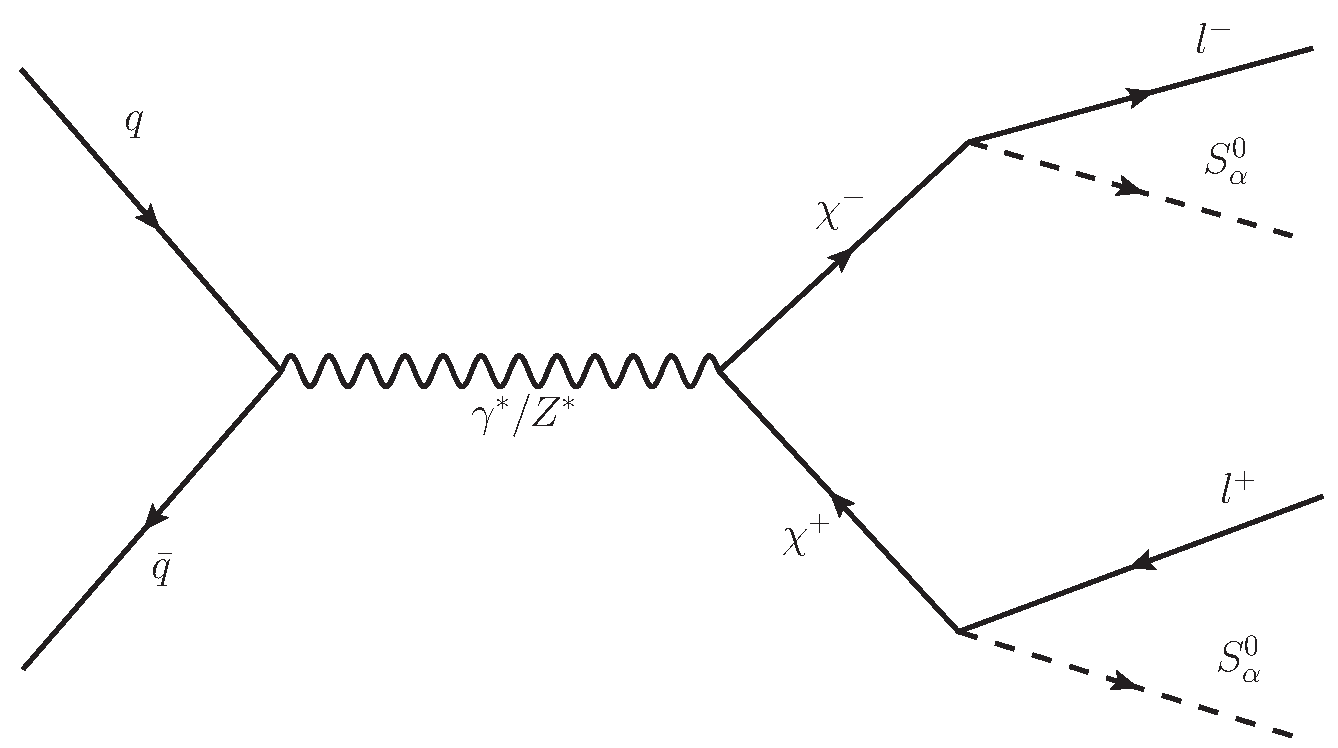
\includegraphics[scale=0.4]{chain1}
\caption{Feynman diagram for $pp \rightarrow \chi^+\chi^- \rightarrow l^+l^- S_{\alpha}S_{\alpha}$ (Drell-Yan process).}
\label{fig:chain_signal}
\end{center}
\end{figure}

In this case, the excluded cross section of this process can be estimated from:

\begin{align}
\label{eq:exccs}
\sigma(pp \rightarrow l^+l^-S_1 S_1)=\sigma(pp \rightarrow \chi^+\chi^-)\times \operatorname{Br}(\chi^{\pm} \rightarrow l^{\pm}S_1)^2 ,
\end{align}
where $\sigma(pp \rightarrow \chi^+\chi^-)$ is the pair production
cross section of charged Dirac fermion, and
$\operatorname{Br}(\chi^{\pm} \rightarrow l^{\pm}S_1)$ is the
branching fraction for $\chi^{\pm} \rightarrow l^{\pm}S_1$
mode.

The pair production of charged Dirac fermions can be
calculated in the pure-higgsino limit of the minimal supersymmetric
standard model. 
The NLO cross section calculated with \texttt{PROSPINO} is displayed
in Fig.~\ref{fig:chargino_production} as a function of the charged
Dirac fermion.

For points in the parameter space where the Casas-Ibarra solution is
chosen such that $\operatorname{Br}(\chi^\pm\to l^\pm\,S_1)\approx 1$,
and assuming the same efficiency as for the dilepton plus missing
transverse energy signal coming from left-sleptons in
Eq.~\eqref{eq:exccs}, the charged Dirac fermions of the present model
can be excluded up to $\SI{510}{GeV}$, as illustrated in
Fig.~\ref{fig:chargino_production}.

\begin{figure}[h]
\begin{center}
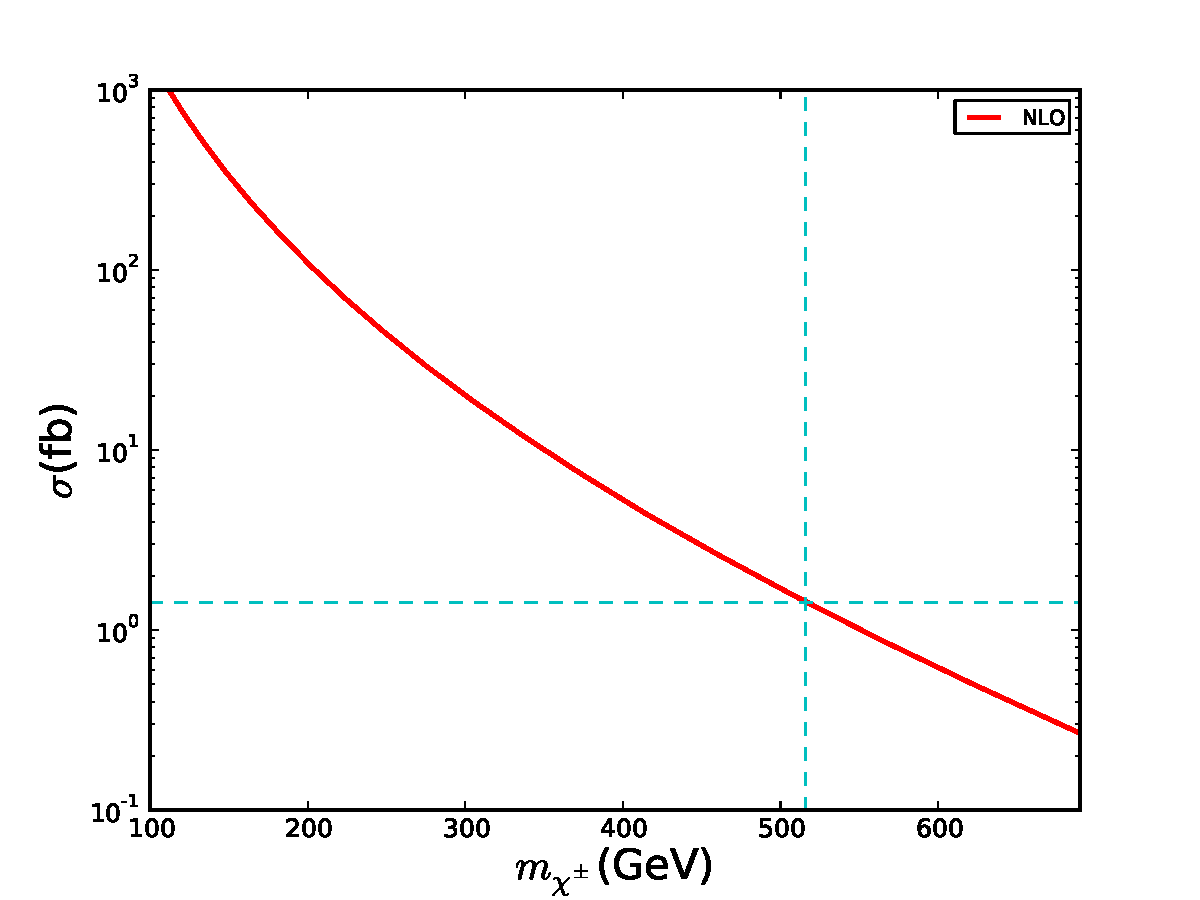
\includegraphics[scale=0.5]{cs2_chacha_prospino}
\caption{NLO cross section for the charged Dirac fermion pair
  production at the LHC with $pp$ collisions at $\sqrt{s}=8$ TeV. 
  The horizontal dashed line for the excluded cross section of
  $\SI{1.4}{fb}$, corresponds to the mass about $\SI{510}{GeV}$
  illustrated by the vertical dashed line.}
\label{fig:chargino_production}
\end{center}
\end{figure}

Note that many points in the scan of Fig.~\ref{fig:brmuegamma} with
$\lambda\lesssim 0.1$ and featuring $m_{S_1}\ll M_D$, could be
excluded by this LHC constraint. 
However, a detailed analysis of the restriction from the Run~I of the
LHC, in the full parameter space of the model, is beyond the scope of this
work.












%%%%%%%%%%%%%%%%%%%%%%%%%%%%%%%%%%%%%%%%%%%%%%%%%%%%%%%%%%%%%%%%%%%%%%%%%%%%%%%%%%%%%%%%%%%%%%%%%%%%
\section{Coannihilation }
\label{sec:singlet-doublet-dark}
In this model, the role of the dark matter particle can be played by
either the lightest of the fermions $\chi_{\text{LOP}}$ or the lightest of the
scalars $S_1$. 
In the latter case, the present model resembles the
singlet scalar DM model
\cite{Silveira:1985rk,McDonald:1993ex,Burgess:2000yq} as long as the
other $Z_2$-odd particles do not contribute to the total annihilation
cross section of $S_1$, namely through to the addition of new
(co)annihilation channels. 
Therefore, by choosing a non-degenerate mass spectrum and small Yukawa
couplings (which is in agreement with neutrino masses) the effects of these particles on dark matter can be neglected. 
Hence, we expect that the dark matter phenomenology to be similar to
that of the SSDM \cite{Cline:2013gha}. 

On the other hand, regarding the case of fermion DM, the present model includes the
singlet doublet fermion DM model
\cite{ArkaniHamed:2005yv,Mahbubani:2005pt,D'Eramo:2007ga,Enberg:2007rp,Cohen:2011ec,Cheung:2013dua}.
In such a scenario, when the dark matter candidate is mainly singlet
(doublet), the relic density is in general rather large (small). 
In particular, a pure doublet has the proper relic density for
$M_{D}\sim\SI{1}{TeV}$~\cite{Mahbubani:2005pt,Cheung:2013dua,Chattopadhyay:2005mv}
with decreasing  values as $M_D$ decreases.  
Nonetheless, in the present model, we have the additional possibility
of coannihilations between the $Z_2$-odd scalars and fermions. 
In this work, we explore at what extent coannihilation with
scalars may allow recovering pure-doublet DM regions with
$M_D\lesssim\SI{1}{TeV}$ and $\lambda\lesssim0.3$ while keeping the
proper relic density.  
Hereafter, we focus in that specific region.


In the simple radiative seesaw model with inert
doublet scalar dark matter, the coannihilations with singlet fermions can enhance
rather than reduce the relic density, as shown in~\cite{Klasen:2013jpa}. That work also presented a review of the several
models~\cite{Servant:2002aq,Kong:2005hn,Burnell:2005hm,Edsjo:2003us,Profumo:2006bx}
where such an enhancement also occurs.
In particular, supersymmetric models where
the neutralino is higgsino-like were considered in~\cite{Profumo:2006bx} and it
was shown that slepton coannihilations not only lead to an increase in
the relic density but also to an enhancement in the predicted
indirect detection signals. 
Below, we show that the singlet scalars can play the role of the
sleptons in our generalization of the higgsino-like dark matter with
radiative neutrino masses.


\begin{figure}
  \centering
  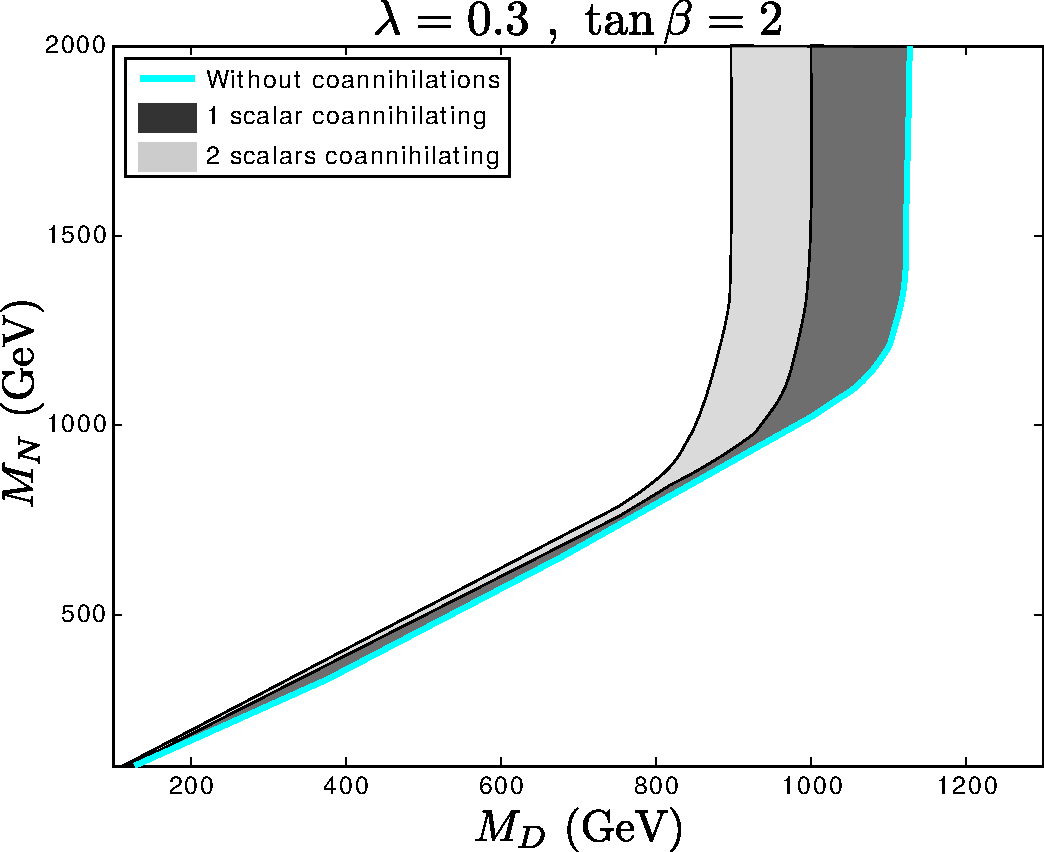
\includegraphics[scale=0.5]{sdfdm}
  \caption{Regions consistent with the observed relic density for $\lambda=0.3$
   and $\tan\beta=2$.    The solid cyan line corresponds to the observed relic density
   without coannihilations which were shown to be compatible with the
   current direct detection bounds from LUX~\cite{Akerib:2013tjd}
   in~\cite{Cheung:2013dua}.
   The effect of the coannihilations with the new scalars is shown for
   a mass degeneracy of 0.1 to 10\% between the scalars and the DM
   candidate. 
   The dark-gray region corresponds to coannihilations with one scalar
   singlet, while the dark plus light-gray regions correspond to
   coannihilations with two scalar singlets.  }
  \label{fig:5b}
\end{figure}


The interactions of the scalars $S_\alpha$ are described by the
$h_{i\alpha}$, $\lambda_{\alpha\beta}^{SH}$ terms in
Eq.~\eqref{eq:lt13a}. 
It turns out that Yukawa interactions are suppressed by neutrino
masses ($h_{i\alpha}\lesssim10^{-4}$) and the same occurs for the interaction
with the Higgs boson if we impose
$\lambda_{\alpha\beta}^{SH}\lesssim10^{-2}$.
In this way, the coannihilating scalars $S_\alpha$ act as parasite
degrees of freedom at freeze-out, leading to an increase of the
singlet-doublet fermion relic density. 

By following the discussion in~\cite{Klasen:2013jpa}, the maximum
enhancement of the relic density is achieved when
$\Delta_{S_\alpha}=(m_{S_{\alpha}}-m_{\text{LOP}}^{\chi})/m_{\text{LOP}}^{\chi}$
becomes negligible. 
Accordingly, one can write
\begin{align}
\frac{  \Omega^{S_{\alpha}}}{\Omega^{0}}\approx\left( \frac{g_0+g_{S_{\alpha}}}{g_0} \right)^2,
\end{align}
where $\Omega^{S_{\alpha}}$ ($\Omega^{0}$) denotes the relic density
with (without) including $S_{\alpha}$ coannihilations,
$g_{S_{\alpha}}$ represents the total number of internal degrees of
freedom related to the scalars participating in the in the
coannihilation process, and $g_{0}$ is the total number of internal
degrees of freedom when $\Delta_{S_\alpha}\gg1$. 
When the DM particle is pure doublet ($M_D\sim1$ TeV and $M_N\gg M_D$),
the fermion masses are $m_1^{\chi}=M_N,\,m_{2,3}^{\chi}\approx
m_{\chi^\pm}=M_D$ and therefore
$g_{0}=g_{\chi_2}+g_{\chi_3}+g_{\chi^\pm}=8$.
Since each real scalar has one degree of freedom, we have
$g_{S_{\alpha}}=1,2,3$ depending on the number of scalars
coannihilating. Thus, it follows that the maximum enhancement is
$\Omega^{S_{\alpha}}/\Omega^{0}=1.27,\, 1.56,\,1.89$, respectively. 
This enhancement results in that, for the present model with
doublet-like DM and $\lambda\lesssim0.3$, the $M_D$ required to explain
the correct relic density lies in the range $[0.9,1.1]$~TeV instead of
taking a single value as in the SDFDM model.  
The values inside this range arise due to no mass-degeneracy
between the fermions and scalars. 
In Fig.~\ref{fig:5b}, we show the effect of coannihilations on the
relic density~\footnote{The relic density is calculated with the
  \texttt{BSM-Toolbox} chain: 
\texttt{SPheno}~3.3.6~\cite{Porod:2011nf}-\texttt{MicrOMEGAs}~4.1.7~\cite{Belanger:2006is,Belanger:2014vza}.}
of $m_{\text{LOP}}^{\chi}$ for a mass degeneracy of 0.1
to 10\% between  scalar singlets and the DM candidate and for
$\lambda=0.3$ and $\tan\beta=2$. 
In particular, in the light-gray region, we plot the coannihilations
with two scalars to facilitate the comparison with the results
in~\cite{Profumo:2006bx} for higgsino-like dark matter coannihilating
with a right-handed stau ($g\approx 2$ in their plots).
As expected, the upper limit in the LOP mass is about $20\%$ smaller
with respect to the case without coannihilation, and we could 
expect similar enhancements for indirect DM searches
as  in ~\cite{Profumo:2006bx} for $g\approx 2$.
Note that, when $M_D,\,M_N<\SI{1}{TeV}$, the impact of the $S_\alpha$ coannihilation is reduced because, in such case, the
dark matter particle is a mixture of singlet and doublet
(well-tempered DM \cite{ArkaniHamed:2006mb}), and the non-negligible
splitting among the fermion particles $\chi$ leads to a non-zero
Boltzmann suppression. 
We have checked that the same results are obtained when
$\lambda\lesssim0.3$.

With regard to DM direct detection in the pure-doublet DM scenario
discussed above, it is not restricted by the current LUX~\cite{Akerib:2013tjd} bounds as
long as $\tan\beta>0$.  
This is due to the existence of zones, known as blind spots, where the
spin-independent cross section vanishes identically and they occur
only for positive values of $\tan\beta$
\cite{Cheung:2013dua}\footnote{Note that $\tan\beta>0$ corresponds to
  $\tan\theta<0$ in notation of  \cite{Cheung:2013dua}.}. 
In consequence, the recovered pure-doublet DM regions are still viable
in light of the present results of direct searches of dark matter.  
%%%%%%%%%%%%%%%%%%%%%%%%%%%%%%%%%%%%%%%%%%%%%%%%%%%%%%%%%%%%%%%%%%%%%%%%







%
\chapter{The \textit{Fermi}-LAT gamma-ray excess at the galactic center in the SDFDM model}

\begin{flushright}
This chapter in based in our work published in \textbf{JCAP03(2016)048}\\ 
\url{doi.org/10.1088/1475-7516/2016/03/048}
\end{flushright}
\begin{center}
\textbf{Abstract}
\end{center}
\InitialCharacter{T}he singlet-doublet fermion dark matter model (SDFDM) provides a good DM candidate as well as the possibility of generating neutrino masses radiatively.
 The search and identification of DM require the combined effort of both indirect and direct DM detection experiments in addition to the LHC.
 Remarkably, an excess of GeV gamma rays from the Galactic Center (GCE) has been measured with the \textit{Fermi}  Large Area Telescope (LAT) which appears to be robust with respect to changes in the diffuse galactic background modeling.
 Although several astrophysical explanations have been proposed, DM remains a simple and well-motivated alternative.
 In this work, we examine the sensitivities of dark matter searches in the SDFDM scenario using \textit{Fermi}-LAT, CTA, IceCube/DeepCore, LUX, PICO and LHC with an emphasis on exploring the regions of the parameter space that can account for the GCE.
 We find that DM particles present in this model with masses close to $\sim 99$ GeV and $\sim (173-190)$ GeV annihilating predominantly into the $W^+W^-$ channel and $t\bar{t}$ channel respectively, provide an acceptable fit to the GCE while being consistent with different current experimental bounds. We also find that much of the obtained parameter space can be ruled out by future direct search experiments like LZ and XENON-1T, in the case of null results by these detectors. Interestingly, we show that the most recent data by LUX is starting to probe the best fit region in the SDFDM model.











\section{The Galactic Center excess in a nutshell }
%
As we described in the section~\ref{sec:intro-gce}, WIMP particles can self-annihilate and for differents mechanisms (one-loop, hadronization) produce High-energy photons in the gamma-ray ($\gamma$-ray) frequency.
Those are the most notable searches channel because they can travel almost unperturbed from their sources to the detectors like the Large Area Telescope on board the \textit{Fermi} satellite (\textit{Fermi}-LAT)~\cite{Fermi}, which is the most sensitive $\gamma$-ray detector in the few GeVs energy range.

The Galactic Center (GC) of the Milky Way Galaxy is expected to be the region displaying the brightest emission of DM annihilations in the $\gamma$-ray sky~\cite{Funk:review}.
However, a multitude of non-thermal astrophysical sources present in that region complicates the identification of a tentative DM signal~\cite{Funk:review}. 
With all this in mind, observations of the inner few degrees around the GC with the \textit{Fermi}-LAT have revealed an excess of $\gamma$-rays ~\cite{Goodenough2009gk,Vitale:2009hr,Hooper:2010mq,hooper,AbazajianKaplinghat2012,AbazajianKaplinghat2013,GordonMacias2013}. 
The spectrum of the Galactic Center excess (GCE) peaks at about 1-3 GeV and its spatial morphology is spherically symmetric varying with radius $r$ around the GC as $r^{-2\gamma}$ with  $\gamma\sim 1.2$, which is clearly compatible with the DM density profile. 
%
This emission has been found to extend out in Galactic latitude ($b$) up to about $|b|\lesssim 20^\circ$ ~\cite{hooperslatyer2013,Daylan:2014,CaloreCholisWeniger2015,TheFermi-LAT:2015kwa} and its presence appears  to be robust with respect to systematic uncertainties~\cite{GordonMacias2013,MaciasGordon2014,Daylan:2014,Zho2015,CaloreCholisWeniger2015,PorterMurgia2015,TheFermi-LAT:2015kwa}.
%
The spatial morphology of the GCE can be accommodated with a Navarro-Frenk-White (NFW) profile with a mildly contracted cusp of $\gamma\sim 1.2$, the measured spectrum implies a WIMP mass in the GeV energy range and an interaction cross section that coincides with the thermal relic cross section. 

A recent study of the GCE~\cite{CaloreCholisWeniger2015} selected a target region ($|b|>2^\circ$) that excluded the core of the GC. Additionally, the systematic uncertainties in the Galactic diffuse emission were estimated in a manner that made the low and high energy tails of the spectrum more uncertain than in previous analyses~\cite{GordonMacias2013,MaciasGordon2014,Abazajian2014,Daylan:2014}, which focused on a smaller region containing the inner $\sim 2^\circ$ of the GC. Although it is possible that the greater degree of uncertainty in the tails found by~\cite{CaloreCholisWeniger2015} is due to an intricate overlap of the GCE with the Fermi Bubbles~\cite{suslatyerfinkbeiner2010,Fermi-LAT:AnnaFranckowiak}, it is interesting that this uncertainty also allows much more freedom for DM models fitting the GCE.

In this chapter, we examine the coverage of WIMP parameter space in the SDFDM model by using mainly indirect and direct DM search techniques in light of the recent detection of the GCE. We show the set of parameters in the SDFDM model that are compatible with the GCE while being consistent with current experimental bounds. Following the same methods explained in Ref.~\cite{Silverwood:2014yza} we compute the expected limits in the annihilation cross-section by the Cherenkov Telescope Array (CTA) and find that observation toward the GC by this instrument will not be able to confirm this model as an explanation of the GCE. However, we find that the viable models can be ruled out by future
direct search experiments such as LZ and XENON-1T, in the case of null results by these detectors. Interestingly, we show that the most recent data by LUX is starting to probe the best fit region in the SDFDM model.











\section{Good self-annihilation channels in the high region of the SDFDM model}
\label{sec:modelgce}

As it was explained in the section~\ref{sec:indirec-detection}, in the SDFDM model DM particles ($\chi^0$) can self-annihilate into $\bar{f}f$, $ZZ$, $W^+W^-$ and $hh$ final states through  $s$-channel Higgs and $Z$ boson exchange and into $ZZ$, $W^+W^-$ states via $t$-channel $\chi_i^0$ and $\chi^{\pm}$ exchange. Annihilations into a mixture of weak gauge bosons $Zh$ are also possible through the exchange of a $\chi_i\neq\chi^0$  in the $t$-channel or a $Z$ in the $s$-channel.  We remark that gamma-ray lines $\gamma\gamma$ and $\gamma Z$ can also be produced at one-loop level. 
%
However, the velocity averaged annihilation cross section $\langle\sigma v\rangle$ of the SDFDM model we have three principal features for indirect detection. First, at low energy the SDFDM model does not exhibit high values for the $\langle\sigma v\rangle$ as it is shown in the left part of Fig.~\ref{fig:good-sv}, 
%
second, at the higher order in scattering theory, the loop suppression leads to small values of the corresponding thermal cross sections \cite{Calibbi:2015nha}, 
%
and third, for DM masses bigger than $m_W$, the $\langle\sigma v\rangle$ exhibit high values as it is shown in the right part of Fig.~\ref{fig:good-sv}.
%
This third feature was one of the prime motivations of the present study. It is clearly shown that the principals channels in the high mass region are the DM self-annihilation into $W^+W^-, ZZ, t\bar{t}$ and $Zh$. 

\begin{figure}[h]
\begin{center}
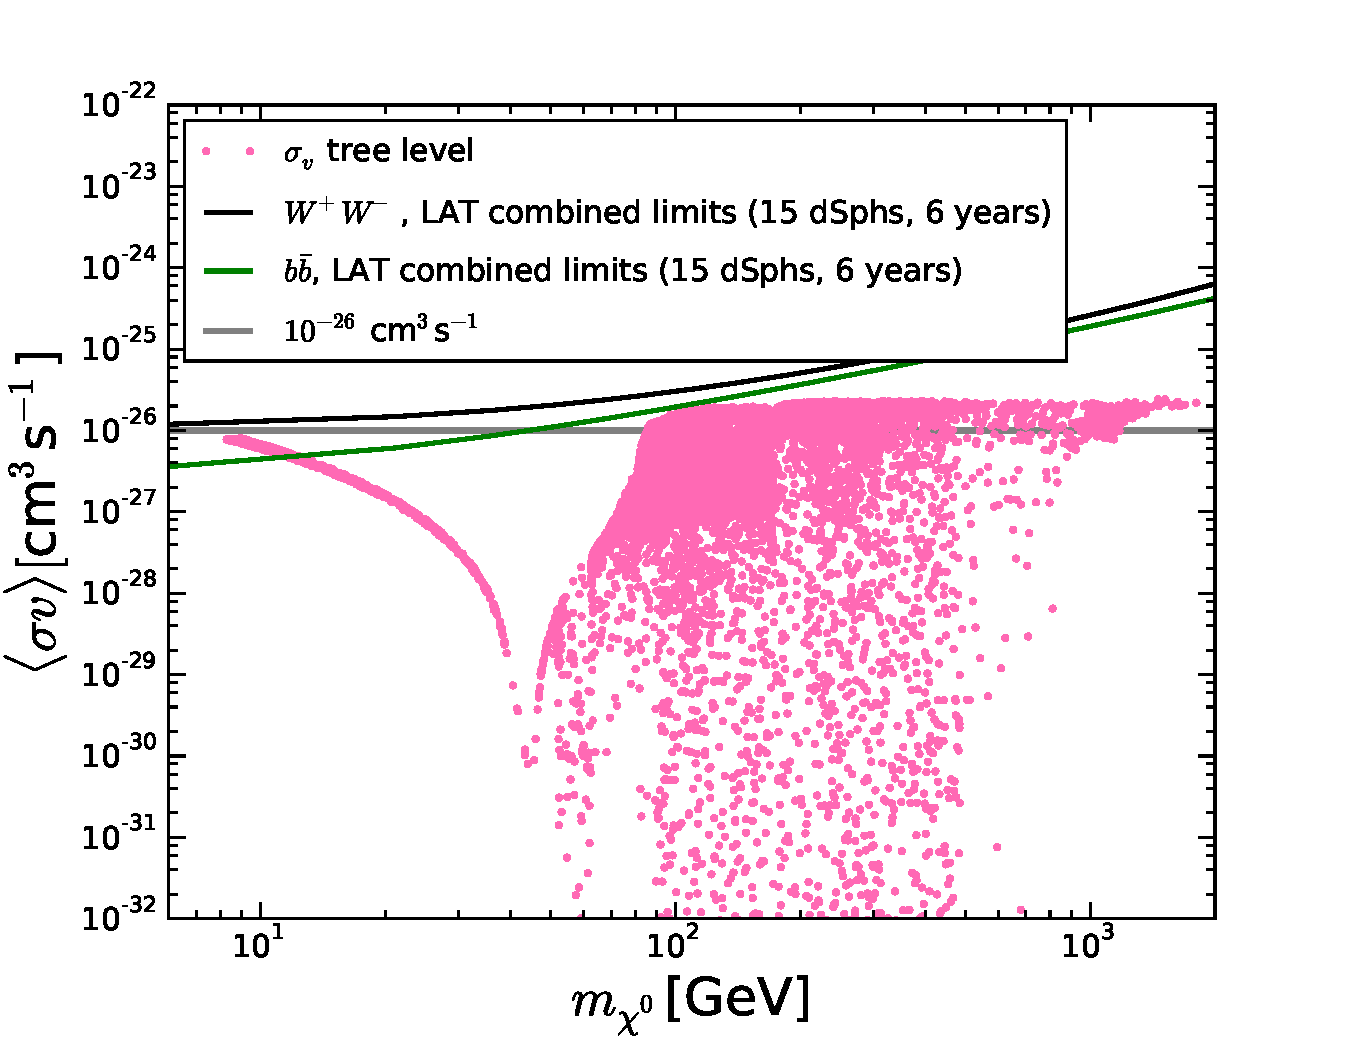
\includegraphics[scale=0.37]{sigmav-T13A}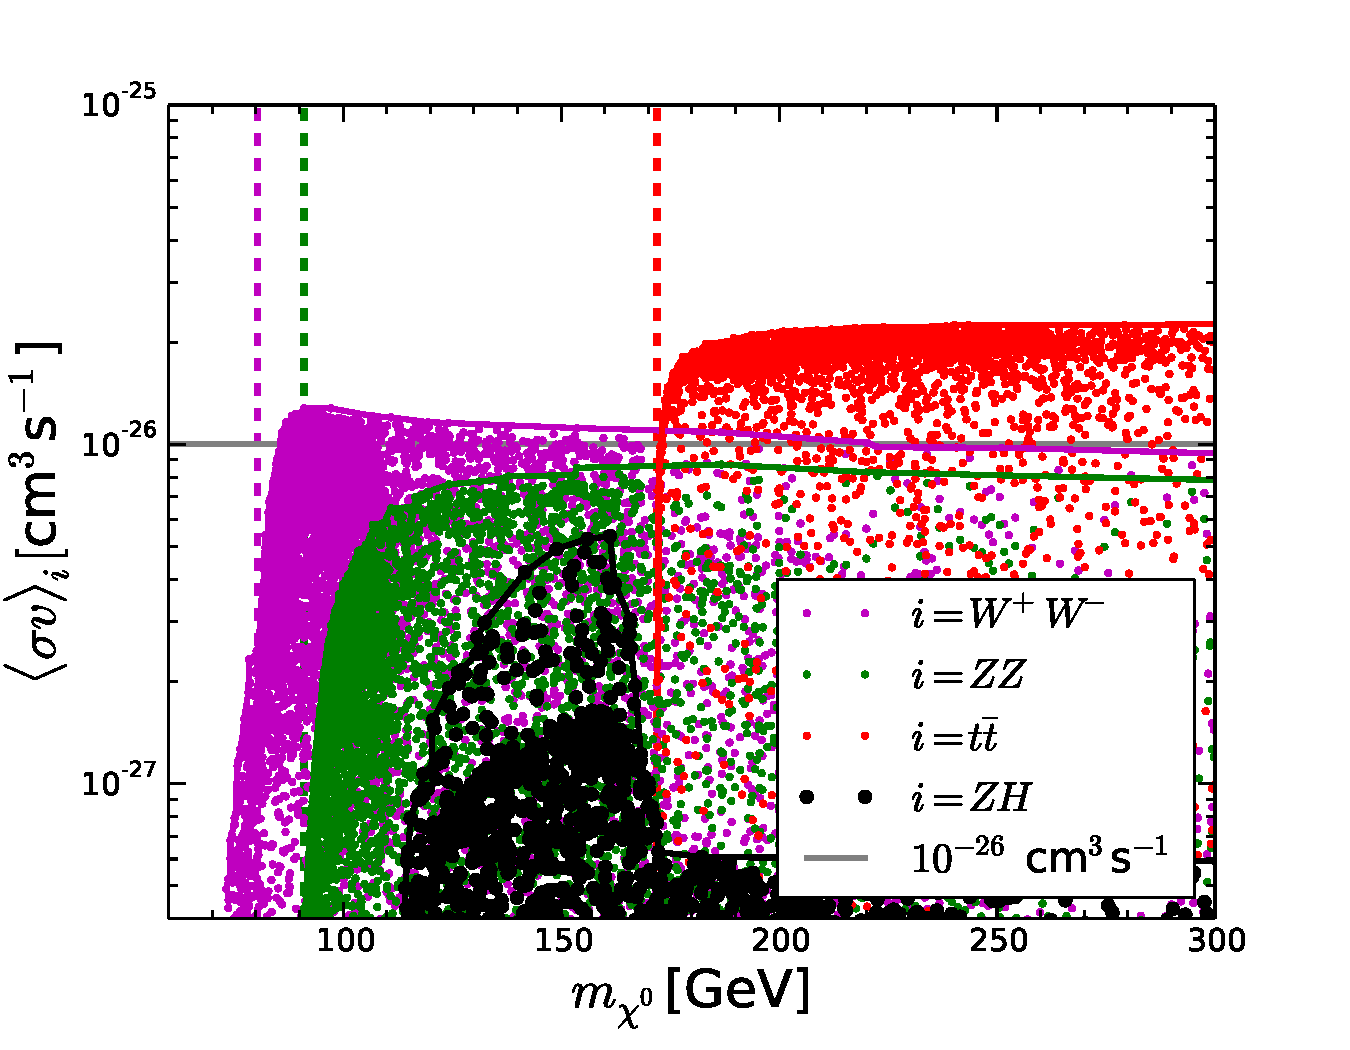
\includegraphics[scale=0.37]{GCE_MDM_vs_canales}
\end{center}
\caption{\textit{Left:} $\langle\sigma v\rangle$ generated randomly for a big sample of the parameters of the SDFDM model (see section \ref{sec:Parameter-scan}). The green (black) line is the current constraint of indirect detection for DM annihilation into $b\bar{b}$ ($W^+W^-$) in the dwarf spheroidal galaxies (dSph)~\cite{Ackermann:2015zua}. The gray line represent the prediction of the WIMP paradigm where the $\langle\sigma v\rangle$ reach the thermal value $10^{-26}\text{cm}^{3}\text{s}^{-1}$. \textit{Right:} Specific region where the $\langle\sigma v\rangle$ reaches the thermal value and the specific channels of DM annihilation.}
\label{fig:good-sv}
\end{figure}











\section{Gamma-rays from the Galactic Center }
\label{sec:gammarays_from_the_GC}
%
The Galactic $\gamma$-ray intensity $\Phi(E_{\gamma},b,l)$ produced in self-annihilations of DM particles, where $b$ and $l$ are the Galactic latitude and longitude respectively, can be obtained from the following relation~\cite{Baltz, Bergstrom,Rott}
\begin{equation}
\Phi(E_{\gamma},b,l)= \frac{1}{2}\frac{\left\langle\sigma v \right\rangle}{4\pi m_{\chi^0}}\sum_{f} \frac{dN_{f}}{dE_{\gamma}}B_f \times J(b,l),
\label{Phi}
\end{equation}
which is the product of a term that depends solely on the inherent properties of the DM particle and an astrophysical factor $J(b,l)$ accounting for the amount of DM in the line of sight.
 The former is given in terms of the velocity averaged annihilation cross-section $\left\langle \sigma v \right\rangle$, the differential $\gamma$-ray multiplicity per annihilation $dN_{f}/dE_{\gamma}$, the DM mass $m_{\chi^0}$ and the branching ratio $B_f$ where $f$ denotes the final state particles resulting from the annihilation. 
The astrophysical factor can be drawn as ~\cite{Bergstrom, Rott}
\begin{equation}
J(b,l)=\int^{\infty}_0 ds\; \rho\left(\sqrt{R^2_{\odot}-2sR_{\odot}\cos(b)\cos(l)+s^2}\right)^2,
\label{J}
\end{equation}
where the DM density-square is integrated along the line-of-sight $s$ and $R_{\odot}=8.25$ kpc is the distance from the solar system to the GC.

The DM halo density $\rho(r)$ is determined by N-body cosmological simulations, with recent studies preferring a generalized NFW profile~\cite{navarrofrenkwhite1997} of the form
\begin{equation}
\rho(r)=\frac{\rho_s}{\left(\frac{r}{r_s}\right)^{\gamma}\left[1+\left(\frac{r}{r_s}\right)^{\alpha}\right]^{(\beta-\gamma)/\alpha}},
\label{nfw}
\end{equation}
where we adopt the scale radius $r_s=23.1$ kpc and the parameters $\alpha=1$, $\beta=3$ as default choices.
 Recent analyses of the GCE~\cite{GordonMacias2013,Daylan:2014,CaloreCholisWeniger2015} find a best fit profile inner slope $\gamma \simeq 1.2$, corresponding to a mildly contracted DM halo.
 We normalized the density profile by fixing the local dark matter $\rho(R_\odot=8.25\; \mbox{kpc})=0.36$ GeV cm$^{-3}$.
 This was done by maximizing the likelihood of microlensing and dynamical data for the chosen profile slope (see Fig.5 of Ref.~\cite{ioccopatobertone2011}). 

The $\gamma$-ray spectra ($dN_{f}/dE_{\gamma}$) resulting from $\chi^0$ annihilations was generated with the software package \textsc{PPPC4DMID} \cite{Cirelli_cookbook}.
 We noticed that for some channels, the interpolation functions provided by this useful tool are incomplete close to the rest mass thresholds.
 In such cases, we instead generated the spectra with the Monte Carlo event generator \textsc{PYTHIA 8.1} \cite{Sjostrand:2007gs} making sure that these were in agreement with the ones in \textsc{PPPC4DMID} for higher mass ranges.
 
Because of the quadratic dependence of Eq.~\ref{Phi} on the dark matter density, the GC is expected to be the brightest DM source in the $\gamma$-ray sky. However, this region also harbors many $\gamma$-ray compact objects and the Galaxy's most intense diffuse $\gamma$-ray emission produced by the interaction of cosmic rays with interstellar material. The impact of these uncertainties in the interpretation of the GCE is currently not very well understood and is the subject of many recent studies.

There are also large uncertainties associated with the predicted signal from DM self-annihilations in the GC. The DM distribution in the innermost region of our Galaxy is poorly constrained by numerical DM-only simulations and kinematic measurements of Milky Way constituents. In principle, ordinary matter is expected to affect the inner dark matter profile obtained from simulations at a certain level. The DM density could be either flattened by star burst activity that ejects baryonic material from the inner region or steepened through adiabatic contraction. Indeed, depending on the assumed DM distribution, different estimates of the expected $\gamma$-ray emission can differ by a factor of up to $\sim 50$ (see Ref.~\cite{Funk:review,Catena:2009mf}).

Dwarf spheroidal galaxies (dSph) of the Milky Way are generally thought to be much simpler targets for indirect DM detection. Although their  $J(b,l)$ factor is orders of magnitude lower than that of the GC, they contain a much cleaner $\gamma$-ray background. Reference~\cite{Ackermann:2015zua} shows that the null detection of $\gamma$-ray emission from such objects imposes strong constraints on the properties of DM models. In the next sections, we will discuss the effects of these limits on the DM interpretation of the GCE. 

Here we entertain the possibility that the SDFDM model can account for the GCE while being consistent with a variety of experimental limits on DM. This is accomplished by following closely the procedure developed in Ref.~\cite{CaloreCholisWeniger2015} and expanded upon in  Ref.~\cite{Caron:2015wda,Bertoneetal}. In summary, the $\gamma$-ray fluxes obtained from our model scans are compared to the GCE data made available in Ref.~\cite{CaloreCholisWeniger2015}. In that work, the systematic and statistical uncertainties in the Galactic diffuse emission model were provided in the form of a covariance matrix $\Sigma_{ij}$, which we use here to the full extent (we refer the reader to the aforementioned article for details on the statistical formalism and the implementation of the $\chi^2$ function). As was done in Refs.~\cite{Caron:2015wda,Bertoneetal}, we modified the covariance matrix to also account for theoretical uncertainties in the $\gamma$-ray spectra generation. Namely, we rewrite $\Sigma_{ij}$ as 
\begin{equation}
\Sigma_{ij} \rightarrow \Sigma_{ij} + \delta_{ij} d^2_{i} \sigma^2_s,
\end{equation}
where $\delta_{ij}$ is the Kronecker delta, $d_i$ are the measured photon fluxes and $\sigma_s=10$\% is the adopted theoretical uncertainty~\cite{Caron:2015wda,Bertoneetal}.


For each of the SDFDM models, we calculate the corresponding $\chi^2$ (or $p$-value) and make sure that these are consistent with the null \textit{Fermi}-LAT detection of $\gamma$-rays in dSphs. As recommended in the 3FGL catalog article~\cite{Acero:2015hja}, a given source spectral model is rejected when its associated $p$-value is less than $10^{-3}$. This is the same as to say that for $24-4$ degrees of freedom ($d.o.f$), model points having a $\chi^2>45.37$ are considered bad fits to the GCE. In all relevant figures, we incorporate the 95\% upper limits on the value of $\left\langle\sigma v \right\rangle$ as extracted from Ref.~\cite{Ackermann:2015zua}.










\section{Numerical analysis}

Having identified the main annihilation channels and established the procedure to calculate the $\gamma$-ray fluxes, we moved to explore the regions of the parameter space that can account for the {\it Fermi} GeV excess. Namely, in this section, we determine the regions that are compatible with current constraints coming from colliders, electroweak phase transition (EWPT), indirect and direct DM searches, and then assess them in light of the quality of the fit to the GCE.  

For this analysis we used the random general scan described in the section \ref{sec:Parameter-scan},    
where each individual model saturates the Planck measurement $\Omega h^2=(0.1199 \pm 0.0027)$~\cite{Ade:2013zuv} at the $3\,\sigma$ level for the relic density. Even more, all the models  are also required to be compatible with \textit{Fermi}-LAT constraints coming from dwarf spheroidal galaxies~\cite{Ackermann:2015zua}, as well as LUX~\cite{Akerib:2013tjd}, IceCube~\cite{2013PhRvL.110m1302A}, PICO-2L~\cite{Amole:2016pye} and PICO-60~\cite{Amole:2015pla}  limits for spin-independent and spin-dependent detection studies, EW precision observables (EWPO) \cite{D'Eramo:2007ga},\cite{Calibbi:2015nha} and searches of charged vector-like particles by LEP~\cite{ALEPH:2005ab}.

%%%%%%%%%%%%%%%%%%%%%%%%%%%%%%%%%%%% PLOT: MD, MN, TANBETA, LAMBDA parameters
\begin{figure}[h]
\begin{center}
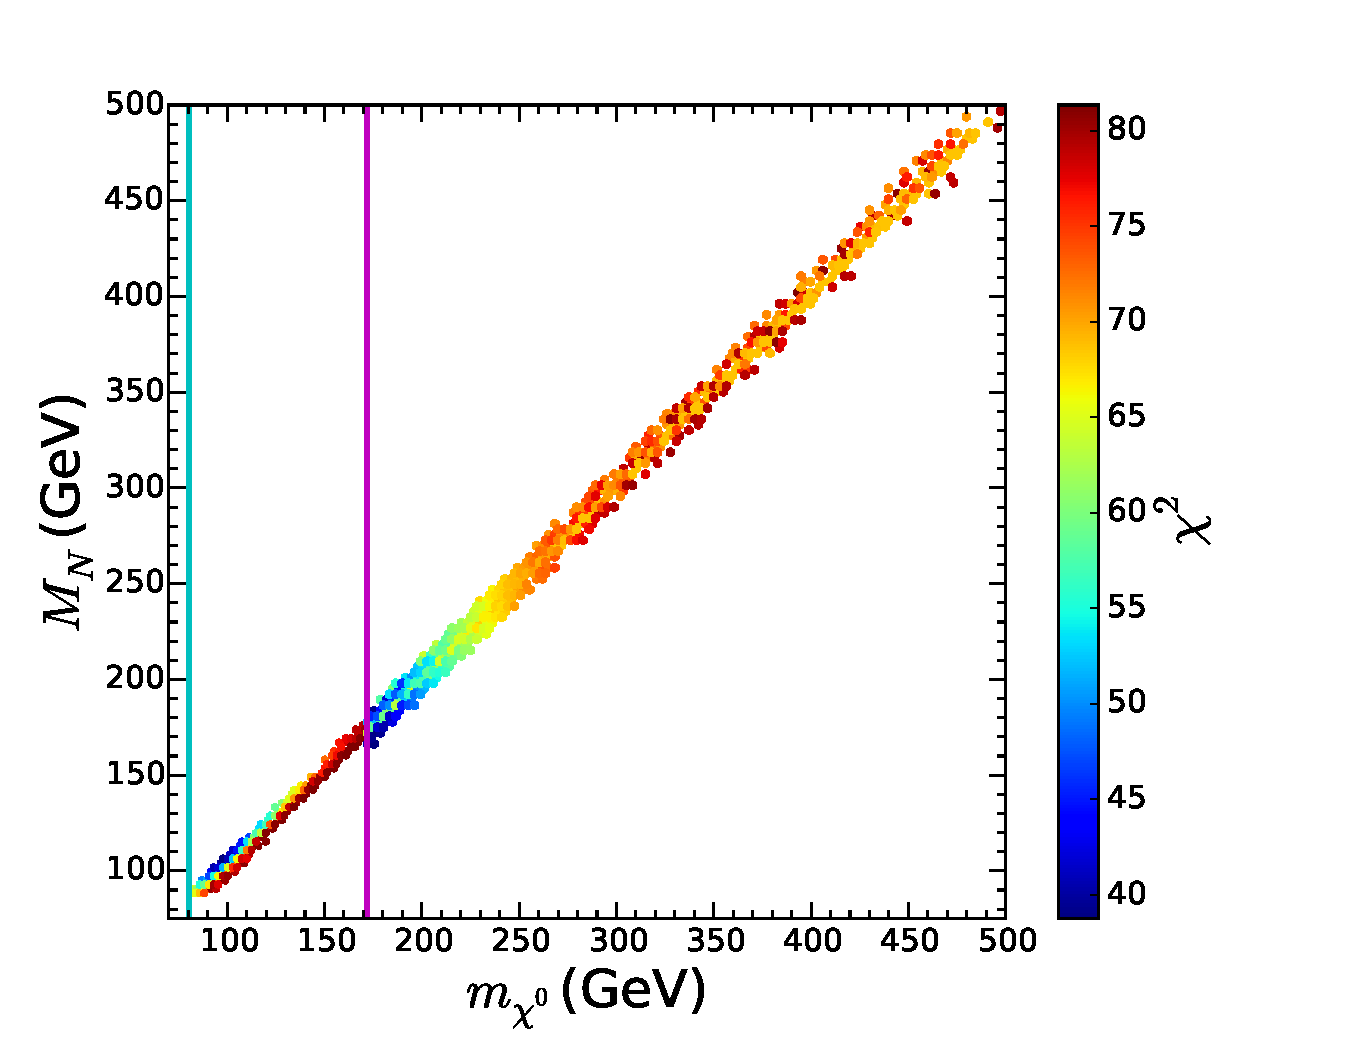
\includegraphics[scale=0.35]{GCE_MDM_vs_MN_2}  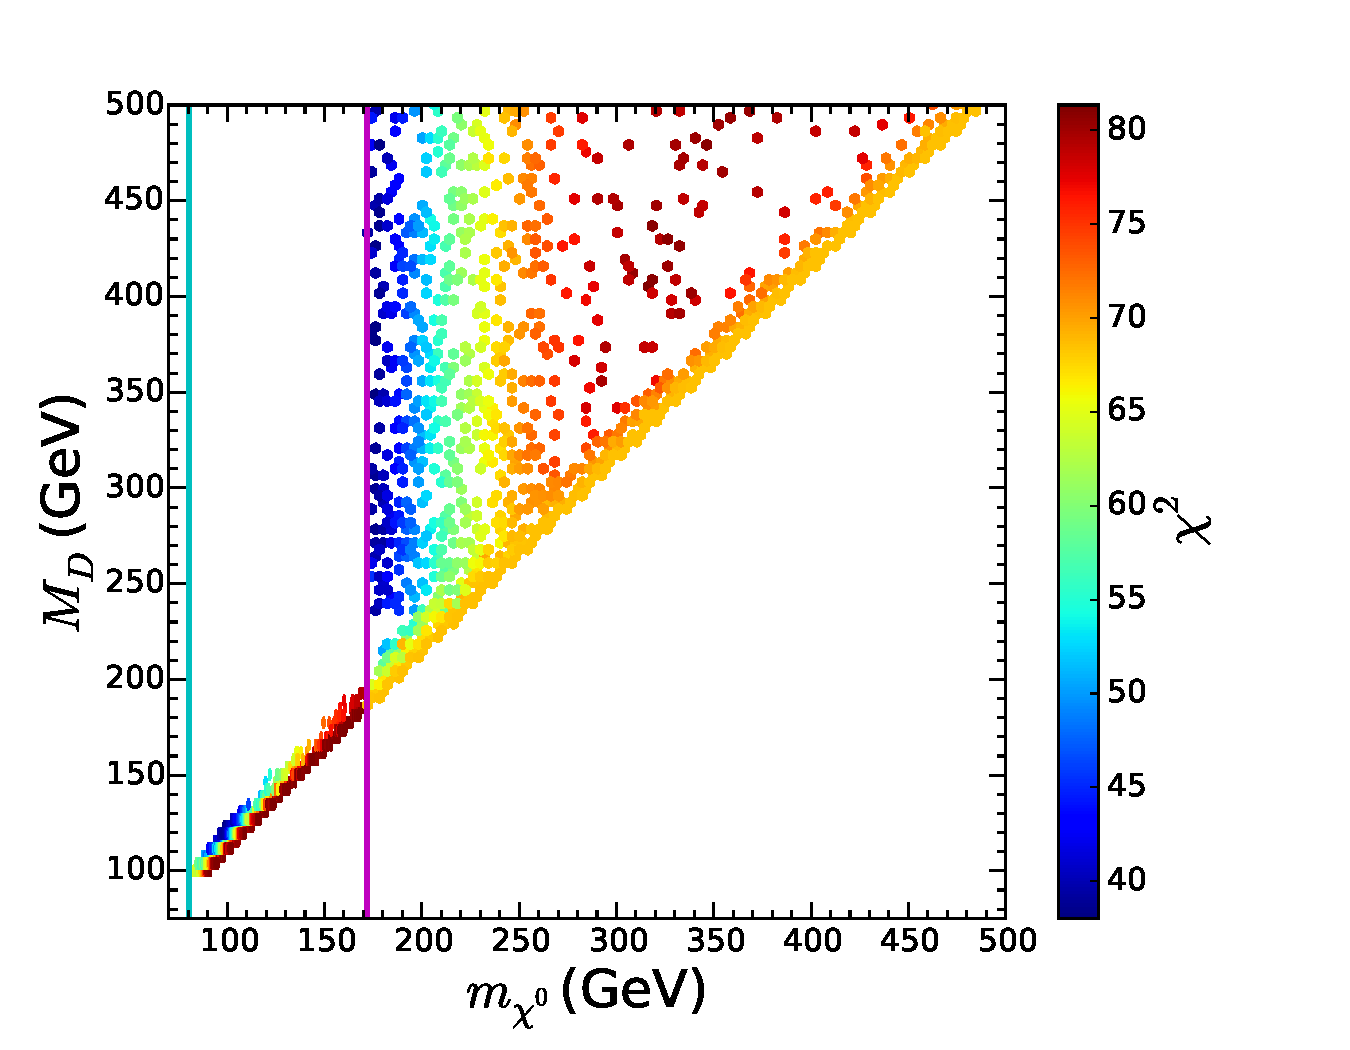
\includegraphics[scale=0.35]{GCE_MDM_vs_MD_2} 
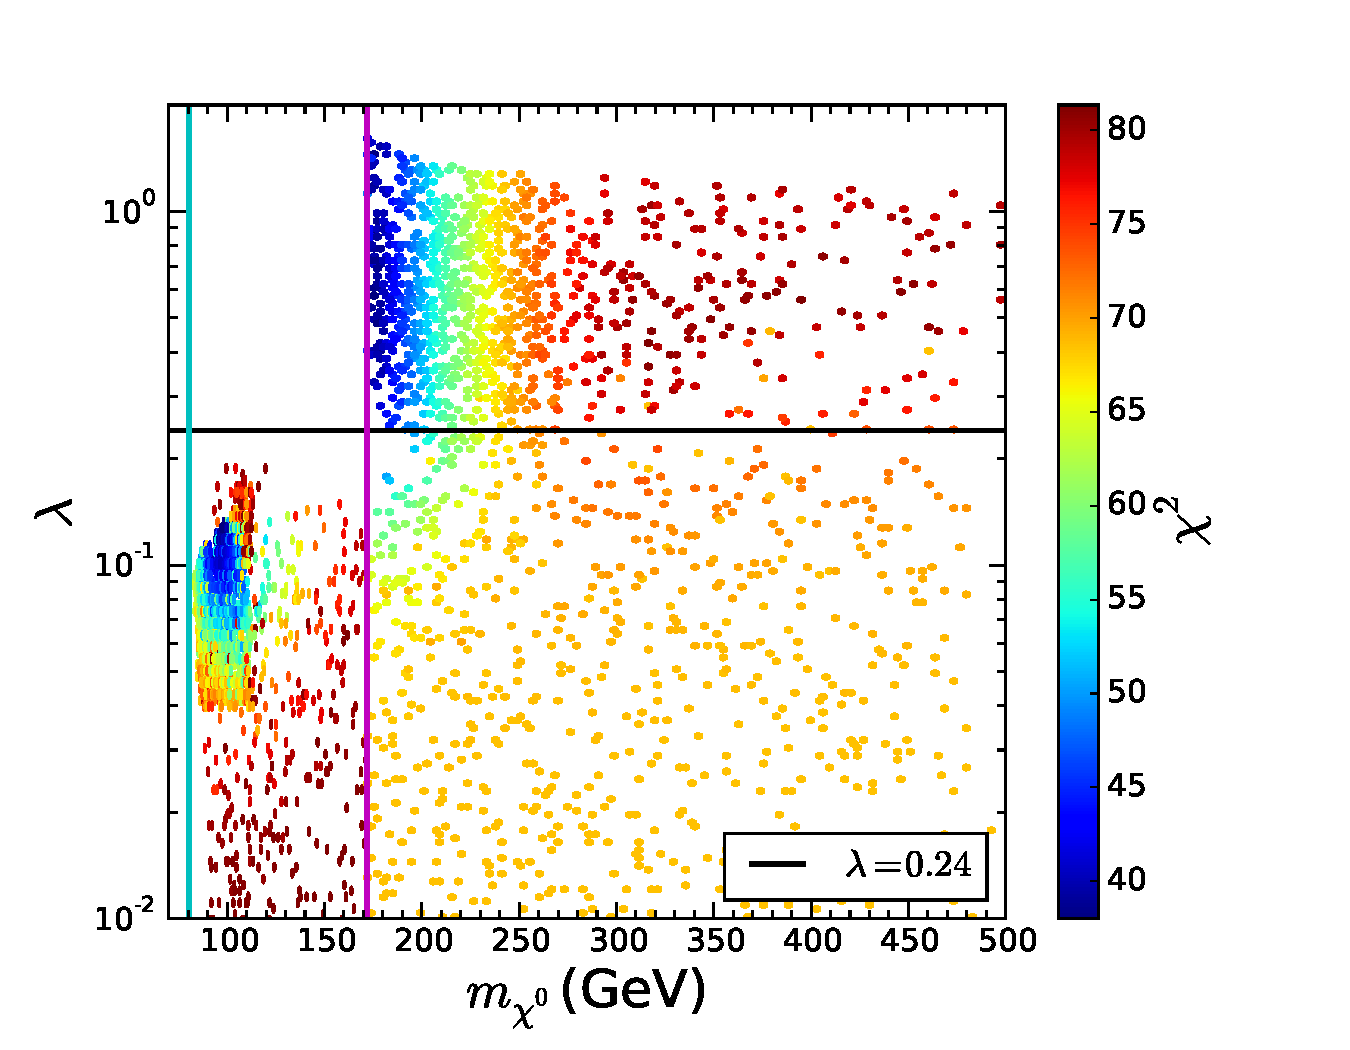
\includegraphics[scale=0.35]{GCE_MDM_vs_lambda_2}  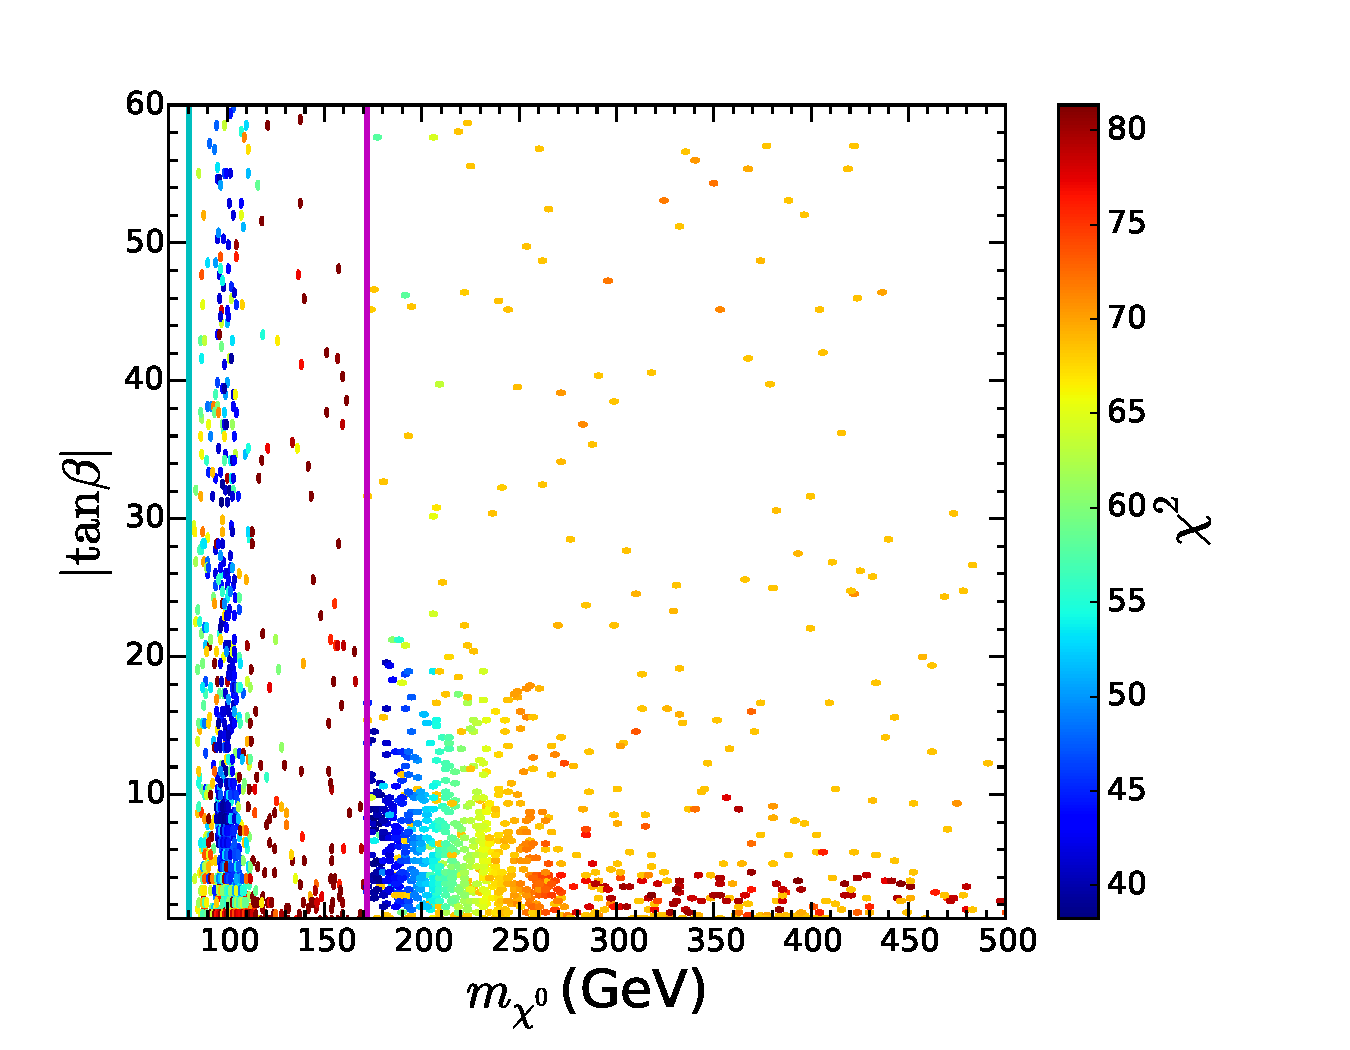
\includegraphics[scale=0.35]{GCE_MDM_vs_tanb_2}
\caption{Two-dimensional projection of the $\chi^2$ values of our fit, showing each one of the four free parameters in the SDFDM model ($M_N$, $M_D$, $\lambda$ and $|\tan \beta|$) versus the dark matter mass ($m_{\chi^0}$). 
In the bottom left panel the black line represents the supersymmetry value $\lambda\sim 0.24$, while the cyan and magenta vertical lines in all panels represent the $W$ boson mass and the top quark mass, respectively. Model points able to fit the GCE are those having a $\chi^2<45.37$ for $24-4$ d.o.f.}
\label{fig:parameters}
\end{center}
\end{figure}
%%%%%%%%%%%%%%%%%%%%%%%%%%%%%%%%%%%%%%%%%%%%%%%%%%%%%%%%%%%%%%%%%%%%%%%%%%%%%












\subsection{Results}
\label{subsec:Results}
Fig.~\ref{fig:parameters} displays the viable models in the planes ($M_N$, $m_{\chi^0}$),  ($M_D$, $m_{\chi^0}$),  ($\lambda$, $m_{\chi^0}$) and  ($|\tan\beta|$, $m_{\chi^0}$), along with the corresponding $\chi^2$ values obtained from a fit to the GCE. 
Since the fit tends to be worse for large values of $m_{\chi^0}$, we only considered DM masses  below 500 GeV. 
Furthermore, as it was discussed in Sec.~\ref{sec:modelgce}, we only studied models with $m_{\chi^0}$ above the $W$ gauge boson mass. 
It is convenient to split the results of our scan into two different regions (DM mass ranges): one in which $m_{\chi^0}$ is below the top mass (Region I) and a second one in which $m_{\chi^0}$ is larger than the mass of the top quark (Region II).  

The viable models belonging to Region I are characterized for having  $M_N\approx M_D\approx m_{\chi^0}$, that is, the DM particle is a mixture of singlet and doublet states (well-tempered DM \cite{ArkaniHamed:2006mb,Cheung:2013dua}). 
The non-observation of direct detection signals constrains the Yukawa coupling to small values ($y<0.2$). We note that this limit excludes the MSSM value $\lambda \sim 0.24$. However, $|\tan\beta|$ is not constrained to a specific value or range. 
Regarding Region II, our analysis shows that $M_N\approx m_{\chi^0}$ while $M_D\gtrsim m_{\chi^0}$. For $y\lesssim 0.3$ the DM particle should be again well tempered ($M_D\approx M_N$) whereas for larger values of $y$ we have that $M_D$ is larger than $M_N$.      
In this case, the upper bound $y\lesssim 5$ comes from the Planck measurement of the DM relic density.

The viable solutions to the GCE found in Region I feature the following parameters: $M_N\sim 105$ GeV, $M_D\sim 120$ GeV, $\lambda\sim 0.12$ and $|\tan\beta|\sim 9$ which generates a DM mass of $\sim 99$ GeV with a $\chi^2$ value of $45.3$. For these parameters the dark matter annihilates mostly into $W^+W^-$. 
While for the Region II we found that the viable solutions correspond to the sample:
\begin{align}
166  < & \, M_N/\text{GeV} < \, 197 , \nonumber \\
236  < & \, M_D/\text{GeV} < \, 988 , \nonumber \\ 
0.25  < & \, \lambda < \, 1.60 ,\nonumber \\
1.87 <  &\, \tan\beta < \, 19.6,
%0.067 <  \, \tan\beta < \, 0.62,&\,\,\,\, \text{and}\,\,\,\, 1.87 <  \, \tan\beta < \, 19.6,
\end{align}
which leads to a DM mass in the range $(173-190)$ GeV with $\langle\sigma v\rangle_{t\bar{t}}/\langle\sigma v\rangle\geq 0.9$ and $\langle\sigma v\rangle_{WW}/\langle\sigma v\rangle\leq 0.1$. The fact that $\chi^0\chi^0\to t\bar{t}$ dominates, via $s$-channel exchange of a $Z$, is reflected in the required values for $y$, because it controls the coupling $c_{Z\chi^0\chi^0}$ whenever $|\tan\beta\neq1|$. 
Note also that, since $\tan\beta>0$ and $\tan\beta\neq1$, the SI and SD cross sections respectively can not be zero (no blind spot occurs). This means that the hypothesis of the SDFDM model being an explanation of the GCE can be probed in future experiments (see next section). Concerning the best $\chi^2$ obtained, we have obtained the value $38.0$ which is represented by the white star in Fig.~\ref{fig:sigmav} and Fig.~\ref{fig:sigma-SI-SD}. 

Overall, the two sets of models capable of explaining GCE have DM particles $\chi^0$ with masses around $99$ GeV and $173-190$ GeV annihilating into $W^+W^-$ and $t\bar{t}$, respectively\footnote{The fact that the DM should annihilate into $W^+W^-$ and $t\bar{t}$ in order to explain the GCE is in accordance with what was stated in Ref.~\cite{Agrawal:2014oha}.}. As explained above, all of our solutions saturate the thermal relic density, making them also consistent with cosmological constraints on dark matter. 








\subsection{Probing the viable solutions with future observations}
%%%%%%%%%%%%%%%%%%%%%%%%%%%%%%%%%%%% PLOT: SIGMAV %%%%%%%%%%%%%%%%%%%%%%%%
\begin{figure}[t]
\begin{center}
\includegraphics[scale=0.5]{GCE_MDM_vs_sigmav_3} 
\caption{The present velocity averaged annihilation cross-section as a function of the dark matter mass in comparison to current indirect detection limits in different channels. 
The 95\% C.L gamma-ray upper limits from dSphs are extracted from Ref.~\cite{Ackermann:2015zua}. The CTA limits correspond to future 100 hr of $\gamma$-rays observations of the GC and assume a generalized NFW profile with an inner slope of $\gamma=1.2$.
The star is the best-fitting model obtained from our scan. 
Vertical lines and color code are the same as in Fig.~\ref{fig:parameters}.}
\label{fig:sigmav}
\end{center}
\end{figure}
%%%%%%%%%%%%%%%%%%%%%%%%%%%%%%%%%%%%%%%%%%%%%%%%%%%%%%%%%%%%%%%%%%%%%%%%%%
The velocity averaged annihilation cross-section as a function of the dark matter mass in
comparison to current indirect detection limits in different channels along with the $\chi^2$ values found in a fit to the GCE are shown in Fig.~\ref{fig:sigmav}. 
Note that current upper limits from dSphs~\cite{Ackermann:2015zua} do not presently constrain any of the viable points. This is a consequence of the imposed requirement that models must comply with the observed DM relic density. Once this condition is applied, it generally restricts the parameter space of the SDFDM model to have a $\langle\sigma v\rangle$ less than $\sim 2\times 10^{-26}$ cm$^3$s$^{-1}$.

Future dSphs analyses with the \textit{Fermi}-LAT telescope will benefit from larger statistics and potential discoveries of new ultra-faint dwarfs. At low energies, the point spread function (PSF) sensitivity for the LAT instrument increases approximately as the square-root of the observation time, while at high energies, the PSF increases roughly linearly with time. The $\gamma$-ray bounds reported in Ref.~\cite{Ackermann:2015zua} used 6 years of \textsc{Pass8} \textit{Fermi} data taken from 15 dwarf spheroidals. Thus, we can conservatively estimate that with 15 years of \textit{Fermi} data and 3 times more dSphs discovered (45 dSphs) in the next few years, the LAT constraints will improve by a factor of $(\sqrt{15}/\sqrt{6})\times 3 \simeq 5$ compared to the current ones. 

As can be seen in Fig.~\ref{fig:sigmav}, the 15 years \textit{Fermi}-LAT forecast in the $W^{+}W^{-}$ channel indicates that future dSphs observations will be in significant tension with the set of favored models found in Region I. Although the \textit{Fermi} collaboration have not yet released equivalent limits for $t\bar{t}$ final states, these should be comparable at the percentage level~\cite{Cirelli_cookbook} with those in the $b\bar{b}$ channel. We thus use the latest limits accordingly, and show that \textit{Fermi}-LAT dwarfs will also have the ability to test our $t\bar{t}$ solution (Region II). However, here an important remark is in order. As discussed in Ref.~\cite{Caloreetal:Taleoftails}, astrophysical uncertainties in the DM parameters can affect the expected $\gamma$-ray emission in a manner that makes the annihilation cross-section uncertain by a factor of $\sim 5$ up and down. Hence, both of our solutions could in principle still escape future \textit{Fermi}-LAT dwarfs limits if astrophysical uncertainties are taken into consideration. Also, as there is likely to be at least some millisecond pulsar contribution, the actual $\langle\sigma v\rangle$ could be correspondingly lower and so even harder to detect.     

Using the method presented in Ref.~\cite{Silverwood:2014yza}, we compute the 95\% confidence level upper limits on the annihilation cross section that will be achievable with the upcoming ground-based $\gamma$-ray observatory CTA~\cite{2011ExA....32..193A}, assuming annihilation into $W^+W^-$ and $t\bar{t}$ channels and the halo model described earlier in this paper. These limits use the 28 spatial bin morphological analysis and include a systematic uncertainty of 1\% and the effects of the galactic diffuse emission. We find the 95\% confidence level upper limits by first calculating the best fit annihilation cross section, and then correctly increasing the cross section until $-2 \ln \mathcal{L}$ increases by 2.71 whilst profiling over the remaining signal model parameters. These limits are shown in Figure~\ref{fig:sigmav}, and show that observations towards the GC by CTA will be unable to confirm or exclude the SDFDM model as an explanation of the GCE. 

%
%%%%%%%%%%%%%%%%%%%%%%%%%%%%%%%%%%%% PLOT: SI , SD  %%%%%%%%%%%
\begin{figure}[h]
\begin{center}
\includegraphics[scale=0.37]{GCE_MDM_vs_sigmaSI_5}\includegraphics[scale=0.37]{GCE_MDM_vs_sigmaSD_5} 
\caption{Spin-independent $\sigma_{SI}$ (left) and spin-dependent $\sigma_{SD}$ (right) direct detection cross sections in the SDFDM model in comparison to current and future direct detection limits. 
The left panel displays current limits from the LUX experiment (black solid line) and the expected limits from the forthcoming XENON-1T and LZ~\cite{Cushman:2013zza} experiments (blue dashed and green dot-dashed lines).
The right panel shows the IceCube limits in the $W^+W^-$ channel (black solid line) from null observations of the sun,  the PICO-2L~\cite{Amole:2016pye} (green light solid line) and PICO-60~\cite{Amole:2015pla} (yellow solid line) limits as well as the LZ sensitivity (green dashed line). The most recent constraints from LUX~\cite{Akerib:2016lao} (red and blue solid lines) are also overlaid. 
The star is the best-fitting model obtained from our scan. 
Vertical lines and color code are the same as in Fig.~\ref{fig:parameters}.
}
\label{fig:sigma-SI-SD}
\end{center}
\end{figure}
%%%%%%%%%%%%%%%%%%%%%%%%%%%%%%%%%%%%%%%%%%%%%%%%%%%%%%%%%%%%%%%
%
The SDFDM model can also be tested through direct dark matter detection searches. This results from either the spin-independent (SI) or spin-dependent (SD) scattering of the $\chi^0$ particle off a target nucleus. Fig.~\ref{fig:sigma-SI-SD} displays the predicted SI and SD cross sections for our model set together with several present and anticipated experimental constraints. Namely, we overlaid the upper limits from the LUX experiment, and the expected limits from XENON-1T and LZ~\cite{Cushman:2013zza}. As can be seen, these future experiments, in particular, LZ, will be able to cut deeply into the model set and confirm or rule out the DM explanation of the GCE if it is the only extended source emitting high energy photons in the GC. 
We also note that available constraints from IceCube are just on the edge of probing the set of models that could account for the excess. In fact, the most recent limits on the spin-dependent WIMP-nucleon elastic cross-section from LUX~\cite{Akerib:2016lao} have begun to disfavor the best-fit region. This is per se, a great example of the importance of a combined effort of different search techniques in the quest for dark matter.    
 

%\section{Conclusions}
%\label{sec:conclusions}
%
%In this work we have entertained the possibility of finding model points in the SDFDM model that can explain the GCE while being in agreement with a multitude of different direct and indirect DM detection constrains. We found two viable regions: (i) DM particles present in the model with masses of $\sim 99$ GeV annihilating mainly into $W$ bosons with branching ratios greater than $\sim 70\%$, (ii) and a second region where the DM particle mass is in the range $\sim (173-190)$ GeV annihilating predominantly into the $t\bar{t}$ channel with branching ratios greater than $\sim 90\%$. Our analysis assumed that the DM is made entirely out of the lightest stable particle $\chi^0$ of the SDFDM model. Despite this being a very restrictive assumption, we have demonstrated that there exist models capable of accounting for the GeV excess in the GC that can be fully tested by the forthcoming XENON-1T and LZ experiments as well as by future \textit{Fermi}-LAT observations in dwarf galaxies. Interestingly, the most recent limits presented by LUX are able to probe a fraction of the good fitting models to the GCE found in this work. We also showed through realistic calculations of CTA performance when observing the GC that this instrument will not have the ability to confirm the SDFDM model if it is causing the GCE.

         



%
\label{sec:gammarays-SDFDM}
\chapter{Dark matter annihilation into two photons}
%
\InitialCharacter{A}fter the freeze-out of the DM, its annihilation continuous but in smaller rate, principally in regions where its concentration is so high, for instance, the center of the Milky Way Galaxy. 
Therefore, exists the possibility to measure this annihilation in flux that reaches the earth.
However, to measure this flux is so challenging because it is typically much smaller than the background flux generated by others astrophysical processes.
Is in this way that one strategy to identify DM signals is to search for gamma-ray spectral features as gamma-ray lines, which are generated directly by the DM annihilation into photons. Fortunately, in the case of the center of the Milky Way Galaxy, DM particles are expected to be very non-relativistic ($v\approx 10^{-3}$) thus generating monoenergetic photons in the annihilation process that are qualitatively very different from the ones expected from the known astrophysical background.
% and for that reason a good form to find signals of DM in the Universe.
It is in this way that searches for gamma-ray spectral features could be competitive for example with direct-detection experiments.  
With this motivation, in this chapter, we compute the cross sections for DM annihilation into two photons for a general model where DM is its own antiparticle and whose stability is guaranteed by the $Z_2$ symmetry. We accomplish this  by carefully classifying all possible one-loop diagrams and reading off the interaction of the DM with the possible mediators from them. Our approach is general and leads to the same results found in the literature for popular dark matter candidates such as neutralino dark matter, minimal dark matter scenarios and Kaluza-Klein dark matter (work in process). The final goal of this chapter is to develop this general scheme that could be useful in the future for indirect-detection studies.
%%SEE INTRODUCTION FO THE ARTICLE for more details










\section{General properties of the annihilation process DM DM $\to \gamma \gamma$}
\label{sec:cond}
In order to systematically study DM annihilations into two photons, we will assume that the DM model satisfies the following conditions: 
%
\begin{enumerate}
\item[\label{condition:i}(i)] DM is its own antiparticle and its stability is guaranteed by a $Z_2$ symmetry. 
\item[\label{condition:ii}(ii)] DM is electrically neutral.
\item[\label{condition:iii}(iii)] As in the SM, additional neutral particles, including the DM, do not couple to two photons at tree level. 
\item[\label{condition:iv}(iv)] In a cubic vertex, photons couple to particles belonging to the same field.  The contribution of possible FCNC is thus neglected. 
\item[ \label{condition:v}(v)] DM has spin zero, one-half or one. 
\item[ \label{condition:vi}(vi)]  The underlying DM theory is renormalizable.
\item[ \label{condition:vii}(vii)]  CP is conserved. 
\end{enumerate}

According to condition~\hyperref[condition:v]{(i)} and~\hyperref[condition:v]{(v)},  DM must be a real scalar, a Majorana fermion or a real vector field. %We write a letter in front for later convenience.  
For each of them, the  amplitude for the process $\text{DM}\text{DM}\to\gamma\gamma$  has  a complicated Lorentz structure. However, exploiting the fact that  we are only interested in non-relativistic DM, %annihilating into photons,  %we will see that for the the parameter space of interest, 
we will show that all the information can be specified by some form factors depending on the spin of the DM.

In the following, $\DM$ is the DM field, $p_i$ and $\sigma_i$  (with $i =3, 4$) stand for the momentum and the helicity of the final state photons in the annihilation process, and $\epsilon_i=\epsilon(p_i,\sigma_i)$ is the corresponding polarization vector. Moreover, we assume vanishing DM relative velocity, $v=0$, and hence  both particles of the initial state have the same four-momentum $p \equiv (\mDM,0,0,0) = (p_3+p_4)/2$.









\subsection{Scalar DM}

In this case, the annihilation amplitude can be cast as
$
{\cal M }_S= {\cal M}^{\mu\nu} \epsilon_{3\mu}^* \epsilon_{4\mu}^*\,.
$
The tensor ${\cal M}^{\mu\nu}$ depends only on $p_3$ and $p_4$ and satisfies $p_{3\mu} {\cal M}^{\mu\nu} = p_{4\nu} {\cal M}^{\mu\nu} =0$ according to the Ward identities. Using this, the property $\epsilon_i\cdot p_i =0$ and the fact that two scalar particles at rest form a CP-even state, 
it can be shown  that  
%
\begin{equation}
  {\cal M}_S ={\cal B} \left( -g^{\mu\nu} + \frac{{p_4}^{\mu} {p_3}^{\nu}}{2\,\mDM^2} \right) \epsilon_{3\mu}^* \epsilon_{4\mu}^*
\,,
\label{eq:Mscalar}
\end{equation}
%
where $\cal B$ is a  scalar function. In terms of this, the cross section reads (see the Appendix~\ref{sec:sigmav})
\begin{equation}
\sigma v \left(\DM\DM \to \gamma\gamma\right) = \frac{|{\cal B}|^2}{32\pi\mDM^2}\,.
\label{eq:cross}
\end{equation}
Hence, for spin-zero DM, our goal is to calculate $\cal B$.






\subsection{Majorana DM}

In this case, we first  write the annihilation amplitude as $\overline{v_1} {\cal M}^{\mu\nu} u_2 \epsilon_{3\mu}^* \epsilon_{4\nu}^*$. That is,  $\cal M^{\mu\nu}$ is the amplitude after stripping out the spinors of the DM particles in the initial state (accordingly, it has spinor indices). This object has more information than we actually need because we are only interested in initial states with  total spin zero. This is because two fermions at rest (i.e. with zero orbital angular momentum) and with total spin one  form a totally symmetric state, which  is  banned for identical particles.  Following Refs.~\cite{Bergstrom:1997fh,Kuhn:1979bb}, we can obtain the amplitude corresponding to the spin-zero initial configuration as
\begin{equation}
\begin{split}
{\cal M}_\text{F} =- \frac{1}{\sqrt2}
\text{Tr} \left\{ {\cal M}^{\mu\nu} \left(\slashed{p}+\mDM\right) \gamma^5 \right\} \epsilon_{3\mu}^* \epsilon_{4\nu}^*\,.
\end{split}
\label{eq:P0}
\end{equation}
%
Similar to the scalar case, gauge invariance and CP conservation restrict the annihilation amplitude. Taking into account that two Majorana particles with no orbital angular momentum form a CP-odd state, we must have 
\begin{equation}
{\cal M}_\text{F} 
%  - \frac{1}{\sqrt2}
%\text{Tr} \left\{ {\cal M}^{\mu\nu} \left(\slashed{p}+\mDM\right) \gamma^5 \right\} 
=\frac{{i\,\cal B}}{2\mDM^2}\,{\epsilon}^{\alpha\beta \mu \nu } {p_{3}}_\alpha {p_{4}}_\beta \epsilon_{3\mu}^* \epsilon_{4\nu}^*
\,.
\label{eq:MMaj}
\end{equation}
%
where $\cal B$ is a  scalar function\footnote{
The overall factor in Eq.~\eqref{eq:MMaj} has been chosen for convenience. In terms of helicities, Eq.~\eqref{eq:MMaj} reads ${\cal M}_\text{F} ={\cal B}\,\sigma_3  \delta_{\sigma_3\,\sigma_4}$. Similarly, 
Eq.~\eqref{eq:Mscalar} reads  ${\cal M}_\text{S} ={\cal B}\, \sigma_3 \delta_{\sigma_3\,\sigma_4}$. Both of them show that the helicities of the final state particles must equal. This can be understood from the fact that the total angular momentum is zero when the DM relative velocity is zero. For scalar particles, this is because there is no spin. For Majorana particles, that follows from the fact that the spin-one state is not possible, as explained above.}, which can be used to calculate the cross section by means of Eq~\eqref{eq:cross} with an extra factor of $1/4$ due to the spin-average of fermions.

\subsection{Vector DM}

In this case, both the initial and final state particles are vector bosons and we can write the amplitude as $
\mathcal{M}_\text{V}=\mathcal{M}_{\mu_1\mu_2\mu_3\mu_4} \epsilon^{\mu_1}_1\epsilon^{\mu_2}_2\epsilon^{\mu_3*}_3\epsilon^{\mu_4*}_4 \,.
$
Assuming at CP-even initial state, as pointed out in Ref.~\cite{Bergstrom:2004nr}, from gauge invariance and Bose statistics it follows that this object can be decomposed as 
%
\begin{align}
\mathcal{M}^{\mu_1\mu_2\mu_3\mu_4} &= 2\left(\dfrac{{\cal B}_2-{\cal B}_6 }{\mDM^4}\right)\,p_3^{\mu_1}p_4^{\mu_2}p^{\mu_3}p^{\mu_4}
+\dfrac{{\cal B}_1}{\mDM^2}g^{\mu_1\mu_2}p^{\mu_3}p^{\mu_4}
-\dfrac{{\cal B}_2}{\mDM^2}g^{\mu_1\mu_3}p_4^{\mu_2}p^{\mu_4}
+\dfrac{{\cal B}_2}{\mDM^2}g^{\mu_1\mu_4}p_4^{\mu_2}p^{\mu_3}\nonumber \\
&+\dfrac{{\cal B}_2}{\mDM^2}g^{\mu_2\mu_3}p_3^{\mu_1}p^{\mu_4}
-\dfrac{{\cal B}_2}{\mDM^2}g^{\mu_2\mu_4}p_3^{\mu_1}p^{\mu_3}
+\dfrac{{\cal B}_6}{\mDM^2}g^{\mu_3\mu_4}p_3^{\mu_1}p_4^{\mu_2}-\frac{1}{2}{\cal B}_1 \, g^{\mu_1\mu_2}g^{\mu_3\mu_4}\nonumber \\
&+{\cal B}_2 \,\left( g^{\mu_1\mu_3}g^{\mu_2\mu_4}
+ g^{\mu_1\mu_4}g^{\mu_2\mu_3}\right)\,.
\label{eq:Mvec}
\end{align}
Hence, our goal is to calculate the function ${\cal B}_1$, ${\cal B}_2$ and ${\cal B}_6$ (we use this notation to keep the conventions of Ref.~\cite{Bergstrom:2004nr} for decomposing the amplitude). In terms of these, the corresponding cross section is given by
\begin{equation}
\sigma v= \frac{1}{576 \pi\mDM^2} \left[3|{\cal B}_1|^2+12|{\cal B}_2|^2+4|{\cal B}_6|^2-4 Re\left( {\cal B}_1 ( {\cal B}_2^*+ {\cal B}_6^*)\right)\right]\,.
\end{equation}

As a closing remark, we would like to comment on the field corresponding to the DM in this case. We can not describe spin-1 DM  by the gauge boson associated to a local symmetry. This is because an ordinary gauge field can not be charged under a $Z_2$ symmetry, as the latter would be explicitly broken. To see this, consider one of the essential ingredients for establishing a local symmetry: the covariant derivate $\partial_\mu + i g A_\mu$. The whole object must transform in the same way under the $Z_2$ symmetry, if this is preserved. However, its  first term is even, while the second one would be odd if we used the gauge field to describe DM, according to condition \hyperref[condition:i]{(i)}.  The condition of renormalizability \hyperref[condition:vi]{(vi)} then implies that we can only use real massive vector fields for our spin-1 DM. 











\section{Classification of the diagrams}
\label{sec:top}

\begin{figure}
\centering
\includegraphics[scale=0.3]{t1}\hspace{-2.4cm}\textbf{T1}\hspace{2.4cm}
\includegraphics[scale=0.3]{t2}\hspace{-2.4cm}\textbf{T2}\hspace{2.4cm}
\includegraphics[scale=0.3]{t3}\hspace{-2.4cm}\textbf{T3}\\
\includegraphics[scale=0.3]{t4}\hspace{-2.4cm}\textbf{T4}\hspace{2.4cm}
\includegraphics[scale=0.3]{t5}\hspace{-2.4cm}\textbf{T5}\hspace{2.4cm}
\includegraphics[scale=0.3]{t6}\hspace{-2.4cm}\textbf{T6}
\caption{Topologies of one-loop diagrams with four external legs.}
\label{fig:topologies}
\end{figure}

\begin{table}[h]
\centering
\begin{tabular}{|lccc|}\hline
Particle & {\bf $Z_2$} & {\bf $U(1)_\text{em}$} & Line\\\hline\hline
$\DM$ & -1 & 0 & \includegraphics[scale=0.2]{../figures/lineDM} \\
$\DMp(\DM^{\pm})$ & -1 & $1$ & \includegraphics[scale=0.2]{../figures/lineDMp} \\
$\medp$ & 1 & $1$ & \includegraphics[scale=0.2]{../figures/linephip}\\
$\medz$ & 1 & 0 & \includegraphics[scale=0.2]{../figures/linephi0}\\\hline
\end{tabular}
\caption{Generic particle content.}
\label{table:mediators}
\end{table}

Conditions \cond  $\,$allow us to classify all diagrams leading to DM annihilation into photons. Eventually, from this classification, we will write down the interaction Lagrangians that give rise to those processes.  
Let us first notice that condition \hyperref[condition:ii]{(ii)}  implies that DM does not annihilate into two photons at tree level. Moreover, as a consequence of requirement \hyperref[condition:vi]{(vi)}, the corresponding one-loop amplitude  must be finite.  

Notice that every one-loop diagram must take the form of one of the topologies shown in Fig.~\ref{fig:topologies}, which we enumerated for later convenience. From condition \hyperref[condition:i]{(i)}, we also know that each diagram must have  a $Z_2$ line starting and ending at the DM particles in the initial state. Moreover, since conditions \hyperref[condition:ii]{(ii)} and \hyperref[condition:iii]{(iii)} forbid the radiation of photons from neutral particles in the diagrams, the fields running in the loop must have electric charge. This means that in addition to the $Z_2$ line, there is closed line in each  diagram  carrying  electric charge.  

According to condition \hyperref[condition:iv]{(iv)}, the electric charge loop is associated to only one field, which we generically call $\DMp$ if it is charged under the $Z_2$ symmetry or $\medp$ in the opposite case. For the sake of simplicity, we assume that  the electric charge of these fields is equal to the  electron charge, however our discussion can be straightforwardly generalized to an arbitrary charge.  
We would like to remark that even though there must be one of these fields in each diagram, we are not restricting ourselves to this minimal content. In fact,   there could be many of these fields in a  given DM theory. Moreover, as we will see later, some diagrams have neutral particles that are even under the  $Z_2$ symmetry and that we generically call $\medz$.  

All these  fields and their quantum numbers are summarized in Table~\ref{table:mediators}, where we also show how we will represent them in Feynman diagrams. In particular, lines associated to the $Z_2$ symmetry are in cyan, whereas, as usual, those associated to the electric charge have an arrow. 
With this assignments, we just proved that every one-loop diagram have a cyan line with its ends in the DM particles in the initial state as well as a loop carrying an arrow. 

Using this observation, we can take each topology in Fig.~\ref{fig:topologies} and assign  fields to its lines by following the next procedure. First, we consider all the possible permutations of the external legs. Second, we draw the lines carrying the $Z_2$ and the electric charge %$U(1)_\text{em}$ 
quantum numbers. Finally, we discard the diagrams that violate one of the conditions stated above. In particular,  according to the requirements \hyperref[condition:ii]{(ii)} and \hyperref[condition:iii]{(iii)},  we will disregard diagrams whose initial legs radiate photons or have neutral particles directly  coupled to two photons.  Interestingly, this procedure %tells us the nature of the mediators involved in the annihilation process and also 
determines the vertices  between the DM and the mediators involved in the annihilation process.  %In fact, our  goal is to determine the Lagrangian associated to these vertices and then calculate the annihilation amplitude from the corresponding Feynman rules. 
%
\newsavebox{\Ta}
\newsavebox{\Tb}
\newsavebox{\Tc}
\newsavebox{\Lagrangian}
\newsavebox{\schLagrangian}
\newsavebox{\Aform}
\newsavebox{\Lagrangianone}
\newsavebox{\Lagrangiantwothree}




%%%%%%%%%%%%%%%%%%%%%%%%%%%%%%%%%%%%%%%%%%%%%%%%

%T1, T2, T3

%%%%%%%%%%%%%%%%%%%%%%%%%%%%%%%%%%%%%%%%%%%%%%%%%%%
%
%
%\begin{table}[h]
\begin{lrbox}{\Ta}
\centering
\begin{tabular}{|c|c|c|}\hline
{\bf Topology} & {\bf Diagrams}% & {\bf Required fields }
 & {\bf Interactions}\\\hline\hline
\multirow{2}{*}{\raisebox{-\height}{\includegraphics[height=2cm]{t1}}}
&
\raisebox{-.5\height}{\includegraphics[height=2.3cm]{figures/t1r1}\includegraphics[height=2.3cm]{figures/t1r2}}
%&$\DM, \DM^\pm, \phi^\pm$
&
\dguno

\\\cline{2-3}
T1
&
\raisebox{-.5\height}{\includegraphics[height=2.3cm]{figures/t1r3}}
%&$\DM, \DM^\pm, \phi^\pm$
&
\dguno

\\\hline
%%%%%%%%%%%%%%%%%%%%%%%%%%%%%%%%%%%%%%%%%%%%%%%
\multirow{2}{*}{\raisebox{-\height}{\includegraphics[height=2cm]{t2}}}
&
\raisebox{-.5\height}{\includegraphics[height=2.3cm]{figures/t2r1}\includegraphics[height=2.3cm]{figures/t2r2}}
%&$\DM, \DM^\pm, \phi^\pm$
&
\dgtres 
\dgdos

\\\cline{2-3}
T2
&
\raisebox{-.5\height}{\includegraphics[height=2.3cm]{figures/t2r3}}
%&$\DM, \DM^\pm, \phi^\pm$
&
%\raisebox{-.5\height}{\includegraphics[height=1.5cm]{dg3}}
\dgcuatro

\\\hline
%%%%%%%%%%%%%%%%%%%%%%%%%%%%%%%%%%%%%%%%%%%%%%%
\multirow{3}{*}{\raisebox{-1.5\height}{\includegraphics[height=2cm]{t3}}}
&
\raisebox{-.5\height}{\includegraphics[height=2.3cm]{figures/t3r1}\includegraphics[height=2.3cm]{figures/t3r2}}
%&$\DM, \DM^\pm, \phi^\pm$
&
\dguno

\\\cline{2-3}
&
\raisebox{-.5\height}{\includegraphics[height=2.3cm]{figures/t3r3}\includegraphics[height=2.3cm]{figures/t3r4}}
%&$\DM, \DM^\pm, \phi^\pm$
&
\dgtres
\dgdos

\\\cline{2-3}
\raisebox{5\height}{T3}
&
\raisebox{-.5\height}{\includegraphics[height=2.3cm]{figures/t3r5}\includegraphics[height=2.3cm]{figures/t3r6}}
%&$\DM, \DM^\pm, \phi^\pm$
&
\dguno
\dgcuatro

\\\hline
\end{tabular}
%\end{table}
%
%
\end{lrbox}






%%%%%%%%%%%%%%%%%%%%%%%%%%%%%%%%%%%%%%%%%%%%%%%%%%%%%%%%%%%%%%%%%%%%%%%%%%

%s-channel: T4 and T5

%%%%%%%%%%%%%%%%%%%%%%%%%%%%%%%%%%%%%%%%%%%%%%%%%%%

\begin{lrbox}{\Tb}
%\begin{table}[h]
\centering
\begin{tabular}{|c|c|c|c|}\hline
{\bf Topology} & {\bf Diagrams} %& {\bf Required fields } 
& {\bf Interactions}\\\hline\hline
\multirow{3}{*}{\raisebox{-1.5\height}{\includegraphics[height=2cm]{t4}}}
&
\raisebox{-.5\height}{\includegraphics[height=2.3cm]{figures/t4r1}\includegraphics[height=2.3cm]{figures/t4r2}}
%&$\DM, \DM^\pm, \phi^\pm$
&
\Ltwelve

\\\cline{2-3}
&
\raisebox{-.5\height}{\includegraphics[height=2.3cm]{figures/t4r3}}%\includegraphics[height=2cm]{figures/t4r4}}
%&$\DM, \DM^\pm, \phi^\pm$
&
\dgcinco \dgseis 
%
\\\cline{2-3}
\raisebox{1.5\height}{T4}
&
\raisebox{-.5\height}{\includegraphics[height=2.3cm]{figures/t4r5}\includegraphics[height=2.3cm]{figures/t4r6}}
%&$\DM, \DM^\pm, \phi^\pm$
&
\Leleven
%
\\\hline
\multirow{3}{*}{\raisebox{-1.5\height}{\includegraphics[height=2cm]{t5}}}
&
\raisebox{-.5\height}{\includegraphics[height=1.7cm]{figures/t5r1}}%\includegraphics[height=2.3cm]{figures/t5r2}}
%&$\DM, \DM^\pm, \phi^\pm$
&
\dgcinco  \dgseis 

\\\cline{2-3}
&
\raisebox{-.5\height}{\includegraphics[height=1.7cm]{figures/t5r3}\includegraphics[height=1.7cm]{figures/t5r4}}
%&$\DM, \DM^\pm, \phi^\pm$
&
\Ltwelve

\\\cline{2-3}
\raisebox{5\height}{T5}
&
\raisebox{-.5\height}{\includegraphics[height=2.9cm]{figures/t5r5}}
%&$\DM, \DM^\pm, \phi^\pm$
&
\Leleven

\\\hline
\end{tabular}
%\end{table}
\end{lrbox}




%%%%%%%%%%%%%%%%%%%%%%%%%%%%%%%%%

% Topology T6

%%%%%%%%%%%%%%%%%%%

\begin{lrbox}{\Tc}
%\begin{table}[h]
\centering
\begin{tabular}{|c|c|c|}\hline
{\bf Topology} & {\bf Diagrams} &% {\bf Required fields } &
 {\bf Interactions}\\\hline\hline
\multirow{4}{*}{\raisebox{-1.7\height}{\includegraphics[height=2cm]{t6}}}
&
\raisebox{-.5\height}{\includegraphics[height=2.3cm]{figures/t6r1}}
&
%$\DM, \DM^\pm, \phi^\pm$&
\Leleven

\\\cline{2-3}
&
\raisebox{-.5\height}{\includegraphics[height=2.3cm]{figures/t6r2}}%\includegraphics[height=2.3cm]{figures/t6r3}}
&
\dgcinco \dgocho
%$...$
\\\cline{2-3}
T6
&
\raisebox{-.5\height}{\includegraphics[height=2.3cm]{figures/t6r4}}
&
%$\DM, \DM^\pm, \phi^\pm$&
\Ltwelve 

\\\cline{2-3}
&
\raisebox{-.5\height}{\includegraphics[height=2.3cm]{figures/t6r5}\includegraphics[height=2.3cm]{figures/t6r6}}
&
%$\DM, \DM^\pm, \phi^\pm$&
\Leleven

\\\hline
\end{tabular}
%\end{table}
\end{lrbox}
%%%%%%%%%%%%%%%%%%%%%%%%%%%%%%%%%%%%%%%%%%%%%%%%%%%%%%%%%%%%%%%%%%%%%%%%%%%%%


%%%%%%%%%%%%%%%%%%%%%%%%%%%%%%%%%%%%%%%%%%
%Lagrangian 
%%%%%%%%%%%%%%%%%%%%%%%%%%%%%%%%%%%%%%%%%%%%%
\begin{lrbox}{\Lagrangian}
	\centering
		\begin{tabular}{|c|c|c|c|c|} \hline
%
\multirow{2}{*}{DM field} & \multicolumn{2}{c|}{\multirow{2}{*}{Mediators}}&  \multirow{3}{*}{\dguno}& \multirow{3}{*}{\dgdos\dgtres}\\
\multirow{2}{*}{ $\DM$}&\multicolumn{2}{c|}{}& &
\\\cline{2-3}
 &\,\,$\medp$\,\,\,&$\DMp$&    & \\\hline\hline
\multirow{3}{*}{Real scalar} & S 
 & S
&$g_1\, \DM \, \DMm  \medp  $
&
$\DM^2 \left(g_2\,  \DMp \DMm + g_3\, \medp \medm\right) $
\\\cline{2-5}
&
F & F
&
$
\, \DM\, \overline{\DMp} \left(g_{1L} P_L 
+g_{1R} P_R\right) \medp
$
&
$0$
\\\cline{2-5}
&
V
& S
&$
i  \, {\medp}^\mu\left(g_{11} \DM {\cal D}_\mu  \DMm +g_{12}{\cal D}_\mu \DM\DMm \right)
$
&
$
 \DM^2 (g_2\, \DMp \DMm +g_3\, \medp_\mu {\medm}^\mu )
$
\\\hline
%
\multirow{3}{*}{Majorana}
& S 
& F
& 
$
\medp \overline{\DM} \left(g_{1L} P_L
+g_{1R} \,P_R \right)\DMm 
$
&
\multirow{3}{*}{0}
\\\cline{2-4}
& F
& S
&
$
\DMm\overline{\DM}\left(g_{1L} P_L +g_{1R} P_R \right) \medp 
$
&
\\\cline{2-4}
& V 
& F
&
$
 \overline{\DM}\medp^\mu \gamma_\mu \left( g_{1L} P_L + g_{1R}  P_R \right)\DMm 
$
&
\\\hline
\multirow{2}{*}{Real vector} &
S
 & S
&
$ i g_1  \,\DM^{\mu}  ( {\cal D}_\mu \DMm \medp - \DMm {\cal D}_\mu \medp) $ 
&

$ \DM_\mu \DM^\mu \left(g_2\,  \DMp \DMm+ g_3\, \medm  \medp\right)$
\\\cline{2-5}
&
F & F
&
$
 \overline{\DMp} \DM^{\mu }\gamma_{\mu }  \left( g_{1L} P_L  
+g_{1R}  P_R \right)\medp
$
&
0
\\\hline
\end{tabular}
\end{lrbox}


%%%%%%%%%%%%%%%%%%%%%%%%%%%%%%%%%%%%%%%%%%
%Lagrangian s-channel 
%%%%%%%%%%%%%%%%%%%%%%%%%%%%%%%%%%%%%%%%%%%%%


\begin{lrbox}{\Aform}
	\centering
		\begin{tabular}{|c|c|c|} \hline
%
\multicolumn{2}{|c|}{\multirow{2}{*}{Mediators}}&  \multirow{3}{*}{\dgseis}\\
\multicolumn{2}{|c|}{}&
\\\cline{1-2}
 \,\, $\medz$\,\,\,&\,\,\,\,\,$\medp$\,\,\,\,\,&     \\\hline\hline
\multirow{3}{*}{CP-even}  
 & S
&$g_6 \medz \, \medm \medp   $
\\\cline{2-3}
& F
&
$g_6 \medz \, \overline{\medp} \medp   $
\\\cline{2-3}
&
V
&
$g_6 \medz {\medm}^\mu{\medp}_\mu$
\\\cline{2-3}
&
Gh
&
$g_6 \medz \, \left(\overline{\med}^-\medp+\overline{\med}^+ \medm \right)   $
\\\hline
\multirow{3}{*}{CP-odd}  
 & S
&$0  $
\\\cline{2-3}
& F 
&
$i g_6 \medz \, \overline{\medp}\gamma_5 \medp   $
\\\cline{2-3}
&
V
&
0 
\\\cline{2-3}
&
Gh
&
$ig_6 \medz \, \left(\overline{\med}^-\medp-\overline{\med}^+ \medm \right)   $
\\\hline
\end{tabular}
\end{lrbox}





\begin{lrbox}{\schLagrangian}
	\centering
		\begin{tabular}{|c|c|c|} \hline
%
%
\multirow{3}{*}{DM field $\DM$} & \multirow{3}{*}{ Mediator $\medz$}&  \multirow{3}{*}{\dgcinco}\\
& & 
\\ &&\\\hline\hline
\multirow{2}{*}{Real scalar} & CP-even  
&$g_5 \medz \DM^2$
\\\cline{2-3}
& CP-odd & 0
\\\hline
%
\multirow{2}{*}{Majorana}
& CP-even  
& 
$
g_5\medz \overline{\DM}\DM
$
\\\cline{2-3}
& CP-odd  
& 
$
i g_5\medz \overline{\DM}\gamma_5\DM
$
\\\hline
\multirow{2}{*}{
Real vector
}
&CP-even  
&
$
g_5 \medz \DM_\mu \DM^\mu
$
\\\cline{2-3}
& CP-odd & 0
\\\hline
\end{tabular}
\end{lrbox}



\begin{table}[H]
\usebox{\Ta}
\caption{Topologies 1, 2 and 3.}
\label{table:T123}
\end{table}

To illustrate the previous procedure, let us first discuss  topologies 1, 2 and 3. The corresponding diagrams are in Table~\ref{table:T123}.   
 None of them violates any of our conditions \cond. In fact, they all arise in the one-loop calculation as long as the interaction vertices listed in front exist. These are
%
\begin{align}&
\raisebox{-.5\height}{\includegraphics[height=2.0cm]{figures/dg1}}\,, &
\raisebox{-.5\height}{\includegraphics[height=2.0cm]{figures/dg2}}\,, \nonumber\\&
\raisebox{-.5\height}{\includegraphics[height=2.0cm]{figures/dg3}}\,,&
\raisebox{-.5\height}{\includegraphics[height=2.0cm]{figures/dg4}}\,.
\label{eq:T123}
\end{align}

%{\color{blue}We will do that in see Sec.~\ref{sec:T345}}

%%%%%%%%%%%% T4 and T5 %%%%%%%%%
\begin{table}[H]
\centering
\usebox{\Tb}
\caption{Topologies 4 and 5.}
\label{table:T45}
\end{table}
%%%%%%%%%%% T6 %%%%%%%%%
\begin{table}[h]
\centering
\usebox{\Tc}
\caption{Topology 6.}
\label{table:T6}
\end{table}

A similar discussion applies to topologies 4, 5 and 6. The corresponding diagrams are shown in Tables ~\ref{table:T45} and ~\ref{table:T6}. In front of each diagram,  we write either the interaction vertices that these diagrams require or if it must be discarded because it violates one of the conditions stated above.  Interestingly, all the viable diagrams that can be constructed out of topologies 4, 5 and 6 correspond to s-channel diagrams involving a neutral particle $\medz$, which couples to the DM at tree-level and that subsequently decays into two photons via a loop of charged particles. Hence,  for these particular topologies, our problem is reduced to calculating the off-shell decay of $\medz$.  We will discuss this more in detail in Sec.~\ref{sec:schannels}. Here, we just mention that for that to be possible  we need the interactions responsible for the production 
 
\begin{align}
\raisebox{-.5\height}{\includegraphics[height=2.6cm]{figures/dg5}}\,,
\label{eq:lscprod}
\end{align}
as well as those associated to the decay
\begin{align}&
\raisebox{-.5\height}{\includegraphics[height=2.5cm]{figures/dg6}} \,,&\raisebox{-.5\height}{\includegraphics[height=2.5cm]{figures/dg8}}\,.
\label{eq:lscdecay}
\end{align}


We arrive to conclusion that, in any DM model satisfying conditions \cond, the annihilation into two photons has an  amplitude  that  can be split into two pieces
\begin{equation}
{\cal B} ={\cal B}\bigg|_{\substack{\text{Topologies}\\\text{1, 2 and 3}}}+{\cal B}\bigg|_\text{s-channel} \,.
\label{eq:Msplit}
\end{equation}  
On the one hand, the first term includes diagrams associated to topologies 1, 2 and 3, which must be calculated by means of the vertices in Eq.~\eqref{eq:T123}. On the other hand,  the second term  is associated to a DM pair exchanging a neutral particle in the s-channel which subsequently decays into photons. Such amplitude requires the vertices in Eq.~\eqref{eq:lscprod} or  Eq.~\eqref{eq:lscdecay}. 


Before closing this section, we would like to remark that
even though the total annihilation amplitude is gauge invariant, that is not necessarily  the case of each piece in Eq.~\eqref{eq:Msplit}. Hence, we have to carefully specify a gauge for our one-loop amplitude. Conditions \cond $ $ also set restrictions on this matter. For fermions or scalars, condition \hyperref[condition:iv]{(iv)} just demands that no FCNC are present. However, for gauge bosons, the situation is more involved because photons could couple to Goldstone and gauge bosons in the same cubic vertex. For instance,  vertices such as $\gamma \,G^+ \,W^-$  are present in linear $R_\xi$ gauges of the SM such as the Feynman gauge (Here, $G^+$ is the Goldstone boson associated to the $W^+$ boson). Nevertheless, as pointed out in Ref.\cite{Bergstrom:1997fh}, in non-linear gauges, condition \hyperref[condition:ii]{(ii)} is satisfied because such vertices are absent~\cite{Fujikawa:1973qs}. We refer the reader to appendix~\ref{sec:Gauge} for a detailed discussion. Here, we just mention that  we  will always work in one of those non-linear gauges.

We can now write down explicitly each of the Lagrangians in Eqs.~\eqref{eq:T123}, \eqref{eq:lscprod} and \eqref{eq:lscdecay}, and calculate the corresponding amplitudes. This is the subject of the following section.










\section{Calculation of the amplitude}
\subsection{Topologies 1, 2 and 3}
\label{sec:T123}

\begin{table}[H]
\usebox{\Lagrangian}
\caption{General interactions.}
\label{table:Lagrangian}
\end{table}

In this section, we calculate the form factors ${\cal B}$ associated to topologies 1, 2 and 3, which lead to the diagrams shown in Table~\ref{table:T123}. To that end, we must specify the spin of both the DM and the mediators, or equivalently, what sort of fields they are, so that we can construct their Lagrangian. %We will be as general as possible. 


Let us start with the DM field.  Condition \hyperref[condition:v]{(v)} implies that DM must be a real scalar, a Majorana fermion or a real vector field. 
With respect to the mediators, we will assume that $\DMp$ is either a complex scalar (S) or a fermionic field (F). Since it is charged under $Z_2$,  we do not consider the possibility of $\DMp$ as a vector boson. Charged spin-1 particles can only be described in a renormalizable way by means of a non-abelian gauge boson, which must not be charged under a $Z_2$ symmetry, as explained above. 

Additionally, we will assume that $\medp$ is a scalar (S), a fermion (F) or a gauge boson (V). Note that Goldstone bosons - which are necessary in the non-linear Feynman gauge- are included in this list. Also, notice that the Padded--Popov ghosts are not considered here because  if they  arose in topologies 1, 2 or 3, DM would directly couple to them, that is, DM would be a gauge boson, a Goldstone particle or a scalar field acquiring a vev; all of which is forbidden by the $Z_2$ symmetry (See Appendix~\ref{sec:Gauge} for more details about  Ghosts in the non-linear gauge). We will see later that ghosts must nevertheless be considered for topologies 4 and 5, which involve s-channel mediators.  We discuss now the interaction Lagrangians.

\subsubsection{Interactions of DM field $\DM$ with  the charged mediators $\DMp$ and $\medp$} 
If we restrict to the previous possibilities, for each of them we can write down the most general Lagrangian associated to the interaction vertices of  Eq.~\eqref{eq:T123}. We show this in Table~\ref{table:Lagrangian}, where the letters S, F and V specify the nature of each field, and stand schematically for scalar , fermionic and vector, respectively. Furthermore, in each case we use generic couplings whose subindex corresponds to the Lagrangian they belong to. Notice that we did not write down the Lagrangians ${\cal L}_4$ of Eq.\eqref{eq:T123}.
This is because gauge invariance demands that these interactions can only arise from the covariant derivative associated to the photon gauge field. 

\begin{comment}
In fact, at it is clear from the table, this only happens for the cases SVS (i.e. scalar DM coupled to a vector field $\medp_\mu$ and scalar DM$^+$) and VSS (vector DM coupled to only scalars). The corresponding Lagrangians are  
%
\begin{align}
{\cal L}_4^{(\text{SVS})} = - ie\,\left(g^{\tiny (1)}_1 +g^{\tiny (2)}_1\right) \text{DM} {\medp}^\mu  \text{DM}^- A_\mu   
+h.c.
%
\\ 
{\cal L}_4^{(\text{VSS})} = - ie\,  \left( g^{\tiny (1)}_{1}+ g^{\tiny (2)}_{1}\right)   \text{DM}^{\mu}\,\medp \text{DM}^-  A_\mu 
+
h.c.
\label{eq:L4}
\end{align}
\CG{Check this!!}
%
\end{comment}
\subsubsection{Interactions of the charged mediators $\DMp$ and $\medp$ with  photons}  
For scalar and fermions, that is trivial as they are described by the usual expressions

\begin{align}
{\cal L}_{\substack{Scalar\\Mediators}} &=  {\cal D}_\mu \medm  {\cal D}^\mu \medp + 
 {\cal D}_\mu \DMm  {\cal D}^\mu \DMp - \mmed^2\, \medm \medp -\mDMp^2\, \DMm \DMp \,,\label{eq:ScalarMediator}
\\
{\cal L}_{\substack{Fermionic\\Mediators}} &=i\overline{\medp}  \slashed{\cal D}\medp +
 i\overline{\DMp}  \slashed{\cal D}\DMp - \mmed\, \overline{\medp} \medp- \mDMp\, \overline{\DMp} \DMp\,. \label{eq:FermionicMediator}
\end{align}
%
where ${\cal D}= \partial - ie A$ is the electromagnetic covariant derivative and $A$ is the photon field. 
The case of the vector mediators $\medp^\mu$ is more complicated. As mentioned above, they must be described by a massive gauge field. Hence, a general approach here is not possible because different gauge groups might lead to different charged vector boson interactions. For concreteness, from now on we will assume that the vector mediator reassembles the $W^+$ boson of the SM. This assumption is not so restrictive as it allows to study DM  with electroweak quantum number as well as other  scenarios where DM interacts with other gauge bosons arising from larger gauge symmetries  such as $W'$ bosons in left-right symmetric theories (See e.g. Ref.~\cite{Heeck:2015qra,Garcia-Cely:2015quu}) or 3-3-1 scenarios (See e.g. Ref.~\cite{TavaresVelasco:2001vb}). Therefore, the vector boson Lagrangian is given by 
\begin{equation}
{\cal L }_{\substack{Vector\\Mediator}}=-\frac{1}{2}\left({\cal D}_\mu \medm_\nu -{\cal D}_\nu \medm_\mu \right)\left({\cal D}^\mu \medp^{\nu} -{\cal D}^\nu \medp^{\mu} \right)+ \mmed^2\, \medm^{\mu}\medp_\mu-ie\,F^{\mu\nu} \medp_\mu\medm_\nu +\delta{\cal L}\, .
\label{eq:VectorMediator}
\end{equation}
where $F$ is the electromagnetic field strength and $\delta{\cal L}$ is the piece of the interaction obtained by the gauge-fixing  procedure in the Feynman non-linear gauge (see Appendix~\ref{sec:Gauge} for details)
\begin{equation}
\delta {\cal L}= 
 - e^2 A^\mu A^\nu  \medm_\mu \medp_\nu
+i  e A^\mu ( \medp_\mu \partial^\nu \medm_\nu-  \medm_\mu \partial^\nu \medp_\nu)\,.
\end{equation}
%
%Notice that, in contrast to the scalar and fermionic case, the interactions of the vector mediator with photons are not uniquely determined by electromagnetic gauge invariance.\footnote{The second term in Eq.~\eqref{eq:VectorMediator} arises in the SM from the $SU(2)$ structure of the electroweak interactions. Even though electromagnetic gauge invariance does not restrict the corresponding coupling for an arbitrary charged vector boson, it has been shown that deviations from the value in Eq.~\eqref{eq:VectorMediator} leads to problems with unitarity~\cite{Ferrara:1992yc}.}


Massive vector fields  come with Goldstone bosons and ghosts. While the latter are not relevant for topologies 1, 2 and 3, the former must be taken into account here. If we were to perform the calculation in any of the usual $R_\xi$ gauges, we would have to also introduce interactions between the Goldstone bosons, the charged vector fields and the photons. Nevertheless, the Goldstone bosons decouple from the gauge field  in the non-linear gauge and therefore in that case the relevant piece of their Lagrangian for our purposes  is simply given by Eq.~\eqref{eq:ScalarMediator} (with $\medp$ as the Goldstone boson).  
 
We are now ready  to calculate the ${\cal B}$ factors  for each scenario of Table~\ref{table:Lagrangian}. To that end, by means of \textsc{FeynRules}~\cite{Christensen:2008py,Alloul:2013bka},  we implement the Lagrangians quoted in this table as well as  those of Eqs.~\eqref{eq:ScalarMediator},\eqref{eq:FermionicMediator} and \eqref{eq:VectorMediator} in \textsc{FeynArts}~\cite{Hahn:2000kx} and \textsc{FormCalc}~\cite{Hahn:1998yk}. Then, we calculate the amplitude for the process DMDM$\to\gamma\gamma$ in each case and have \textsc{FormCalc} to reduce their tensor integrals to scalar Passarino-Veltman functions.
%%%% PONER REFERECIA
% {\color{blue}(See e.g. for a review on this procedure, see e.g. )}. 

Unfortunately, for relative DM velocities approaching zero, i.e. $v\to0$, the previous algorithm for reducing the  tensor integrals in the amplitude to scalar functions leads to numerical inestabilities and even breaks down for $v=0$. This pathological behavior is well-understood and stems from the assumption that the external momenta in the annihilation process are linearly independent. Following~\cite{STUART1988367}, we reduce the integrals dropping such assumption. For a detailed description of this procedure, we refer the reader to Appendix~\ref{sec:CD-reduction}.
%%% MY FINAL TEXT 
Specifically, this algorithm reduces the four-point function to three-point functions. Later, we used the \textsc{Package-X}~\cite{Patel:2015tea} to reduce all the remaining coefficients tensor $C_{\mu},C_{\mu\nu},C_{\mu\nu\rho}, \cdots $, to the scalar Passarino Veltman $C_0$~\cite{Passarino:1978jh}. Usually, the results are given in terms of $C_0$ which can be given in terms of the dilogarithm Li$_{2}$ functions. However, in the case of $C_0$, the notation is more compact and readable.

In Sec.~\ref{sec:cond}, based on general considerations such as Lorentz and gauge invariance, we argued that the annihilation amplitude can be cast as shown in Eqs.~\eqref{eq:Mscalar}, \eqref{eq:MMaj} and \eqref{eq:Mvec}. Using the previous procedure, we explicitly  corroborate  that. Furthermore, for a given set of interactions ${\cal L}_1$, ${\cal L}_2$ and ${\cal L}_3$, we can decompose each form factor in terms of Passarino-Veltman functions of two and three points describe in the Appendix~\ref{sec:passarino-veltman}. Concretely,

\begin{align}
%\label{eq:passarino-components}
{\cal B}\bigg|_{\substack{\text{Topologies}\\\text{1, 2 and 3}}}= \dfrac{\alpha}{\pi}\bigg[% {\color{red}\dfrac{x_1}{3(\rmed^2-\rDMp^2+1)}
&x_1 
+x_2 \dfrac{ \, C_0( 0, 1, -1, \rmed ^2, \rmed ^2, \rDMp^2)  }{(\rDMp^2-\rmed^2)(1+\rDMp^2-\rmed^2)}
+x_3 \dfrac{ \, C_0( 0, 1, -1, \rDMp^2, \rDMp^2, \rmed ^2)}{\left(-\rDMp^2+\rmed^2\right)\left(1-\rDMp^2+\rmed^2\right)}\nonumber\\
&+x_4 \,\, C_0\left( 0, 4 \, , 0, \rmed ^2, \rmed ^2, \rmed ^2\right)
+ x_5 \,\,  C_0\left( 0, 4 \, , 0, \rDMp^2,\rDMp^2, \rDMp^2 \right)\nonumber\\
&+x_6\, \left(B_0(4 , \rmed^2 ,\rmed^2 )- B_0(1 ,\rDMp^2, \rmed^2 )\right)\nonumber\\
&+x_7\, \left(B_0(4 , \rDMp^2,\rDMp^2)- B_0(1 ,\rDMp^2, \rmed^2 )\right)\nonumber\\
&+x_8\, \left(B_0(-1 , \rDMp^2,\rmed^2 )- B_0( 1,\rDMp^2, \rmed^2 )\right)%
%-(x_6+x_7)\, B_0( , \rmed ,\rDMp)
\bigg]\,,%\nonumber
\label{eq:B123expansion}
\end{align}

\begin{comment}
\begin{align}
%\label{eq:passarino-components}
{\cal B}_\text{T123}= \dfrac{\alpha}{\pi}\bigg[% {\color{red}\dfrac{x_1}{3(\rmed^2-\rDMp^2+1)}
&x_1 
+x_2 \dfrac{ \mDM^2\, C_0( 0, \mDM^2, -\mDM^2, \mmed^2, \mmed^2, \mDMp^2)  }{(\rDMp^2-\rmed^2)(1+\rDMp^2-\rmed^2)}
+x_3 \dfrac{ \mDM^2\, C_0( 0, \mDM^2, -\mDM^2, \mDMp^2, \mDMp^2, \mmed^2)}{\left(-\rDMp^2+\rmed^2\right)\left(1-\rDMp^2+\rmed^2\right)}\nonumber\\
&+x_4 \,\mDM^2\, C_0\left( 0, 4 \, \mDM^2, 0, \mmed^2, \mmed^2, \mmed^2\right)
+ x_5 \,\mDM^2\,  C_0\left( 0, 4 \, \mDM^2, 0, \mDMp^2,\mDMp^2, \mDMp^2 \right)\nonumber\\
&+x_6\, \left(B_0(4 \mDM^2, \mmed,\mmed)- B_0( \mDM^2,\mDMp, \mmed)\right)\nonumber\\
&+x_7\, \left(B_0(4 \mDM^2, \mDMp,\mDMp)- B_0( \mDM^2,\mDMp, \mmed)\right)\nonumber\\
&+x_8\, \left(B_0(- \mDM^2, \mDMp,\mmed)- B_0( \mDM^2,\mDMp, \mmed)\right)%
%-(x_6+x_7)\, B_0( \mDM^2, \mmed,\mDMp)
\bigg]\,,%\nonumber
\label{eq:B123expansion}
\end{align}
\end{comment}
%
where $\rmed \equiv \mmed/\mDM$, $\rDMp \equiv \mDMp/\mDM$  and $x_i$ are dimensionless coefficients for different combinations of mediators. The same expression holds for $\mathcal{B}_1$, $\mathcal{B}_2$ and $\mathcal{B}_6$ in the case of vector DM.
The goal of this work is to compute all the $x_i$ coefficients for each model (work in process). In this thesis, as an illustration, we only will apply this schema to two particular examples in the Sec.~\ref{sec:two-examples}.











\subsection{Topologies associated to s-channels }
\label{sec:schannels}

\begin{table}[H]
\begin{centering}
\begin{minipage}{0.44\textwidth}
\usebox{\schLagrangian}
\caption{Interactions of $\DM$ with neutral mediators.}
\label{table:schLagrangian}
\end{minipage}
\hspace{40pt}
\begin{minipage}{0.44\textwidth}
\usebox{\Aform}
\caption{Interaction among neutral and charge mediators.}
\label{table:Acal}
\end{minipage}
\end{centering}
\end{table}

As for previous topologies, we must first specify the nature of the particles involved in the annihilation diagram. Tables~\ref{table:T45} and \ref{table:T6} clearly show that the particle in the s-channel is a boson  electrically neutral and even under the $Z_2$ symmetry. 
In Appendix~\ref{sec:Gauge}, we prove that if the particle on the s-channel is a massive gauge boson, its contribution to the annihilation vanishes in the Landau gauge, and only the corresponding  (massless) Goldstone boson must be taken into account. Thus, without loss of generality, we will only consider the possibility of a scalar particle on the s-channel. Furthermore, because we are assuming that CP is conserved, we can classify the the possible s-channel diagrams according to the CP-parity of the scalar mediator.

Using this,  we divide the problem in two parts. On the one hand, we describe how the DM couples to the neutral mediator. This information is carried by the Lagrangian ${\cal L}_5$ of Eq.~\eqref{eq:lscprod}, which we write in  Table~\ref{table:schLagrangian} for each type of DM.  On the other  hand, we describe the off-shell decay of the mediator.  This is done by means of the Lagrangian ${\cal L}_6$ of Eq.\eqref{eq:lscdecay}, which we specify in Table~\ref{table:Acal} for all the possible charged mediators.  Notice that ${\cal L}_7$ vanishes\footnote{This only true if we demand that the charged particles in ${\cal L}_7$ belong to the same field. We do that because we want to satisfy condition~\hyperref[condition:iv]{(iv)} for closing the loop. If we drop this requirement, ${\cal L}_7$ does not vanish. For instance, if the particle in the s-channel is the Higgs boson, vertices such as $h W^+G^-\gamma $ would contribute to the annihilation into photons because the vertex $W^+G^- \gamma$ exists in general (for clearer picture, see the second row of Table~\ref{table:T6}). As discussed previously, in order to avoid these situations, we work in the non-linear Feynman gauge where the latter vertex does not exist.}. In contrast to case of topologies 1, 2 or 3, here we do need to take into account the presence of Ghosts because a scalar particle can interact with them if it also couples to charged gauge bosons. Notice that for each charged gauge boson, there are two  Ghosts, as shown in the Table.  

Combining the information on Tables~\ref{table:schLagrangian} and \ref{table:Acal}, we can calculate the annihilation amplitude for any s-channel process. 
%In analogy to Eq.~\eqref{eq:B123expansion}, for each set ${\cal L}_5$ and ${\cal L}_6$, we find
%
%\begin{align}
%{\cal B}\bigg|_\text{s-channel}= \dfrac{\alpha}{\pi}\bigg[
%&x_9 
%+x_{10}\, C_0\left( 0, 4 , 0, r_{\medp}^2,  r_{\medp}^2,  r_{\medp}^2\right)
%\bigg]\,.%\nonumber
%\label{eq:Bschexpansion}
%\end{align}
%%The coefficients for each case listed in the tables  are found in Appendix~\ref{sec:xs}. 
%
% Before finalizing this section,  w
We discuss the case the Higgs and the $Z$ boson as s-channel mediators. They are very important not only because they arise in many DM models but also because we know their couplings to SM particles and consequently their contribution to the annihilation amplitudes can be calculated precisely.
\begin{itemize}
\item $\medz$ as the Higgs boson. If SM scalar doublet is given by
\begin{equation}
H = \begin{pmatrix} G^+ \\ \frac{v+h +i G^0}{\sqrt{2}}\end{pmatrix}\,,
\end{equation}
the relevant couplings of Table~\ref{table:Acal} are  
\begin{equation}
g_6=
\left\{
\begin{array}{ll}
-\frac{m_h^2}{v}   &\text{for }\medp=G^+,\\
-\frac{m_f}{v}  &\text{for }\medp=\text{any SM fermion,}\\
+\frac{2 m_W^2}{v} &\text{for }\medp = W^+,\\
-\frac{m_W^2}{v} &\text{for the ghosts of }W^+.\\
\end{array}
\right.
\end{equation}
%
For scalar DM annihilating into photons via the Higgs on the s-channel, we found that the $\mathcal{B}$ factor is given by
%we can compute the amplitude by plugging the computed %$x_9$ and $x_1$ coefficients into the Eq.~\eqref{eq:Bschexpansion}. We find
%
\begin{eqnarray}
{\cal B}^h_\text{SM}\bigg|_\text{s-channel} &=&\frac{g_5 \alpha}{\pi v}  \left[\underbrace{ m_h^2 \left( 1-r_W^2 f_W\right)}_{\text{loop of $G^+$} } \underbrace{-4 \mDM  \sum_f  Q_f^2\, N_f\, m_f r_f \left( 1- (r_f^2-1)f_f\right)}_{\text{loop of SM fermions} } \right.\\
&&\left.
+ \underbrace{8 m_W^2\left(1-(r_W^2-2)f_W \right)}_{\text{loop of $W^+$} } \underbrace{-2  m_W^2\left(1-r_W^2f_W \right)}_{\text{loop of ghosts} }\right]\frac{1}{4\mDM^2-m_h^2+i\Gamma_h m_h}\nonumber\,,
\label{eq:schHiggslike0}
\end{eqnarray}

where we scale the fermions contribution with their electric charge and number of colors, $r_f=m_f/\mDM$, $r_W=m_W/\mDM$,  and  introduce a common way of expressing the Passarino-Veltman function
\begin{equation}
f_{\med} = -2 \, C_0\left( 0, 4 , 0, \rmed^2,  \rmed^2,  \rmed^2\right)\,.
\end{equation}
Moreover, if we define
\begin{align}
A^h_1(r_W) = -(2+3r_W^2)- 3(2-r_W^2)r_W^2 f_W & \,, & A^h_{1/2}(r_f) =  2\,r_f^2\left( 1-(r_f^2-1)f_f\right) \,,
\end{align}
and notice  that $\alpha\, m_h^2 = -\alpha(4\mDM^2-m_h^2+i\Gamma_h m_h)+  4\alpha\, \mDM^2+ {\cal O}(\alpha^2)$, Eq.~\eqref{eq:schHiggslike0} can be cast in a more compact form
\begin{eqnarray}
{\cal B}^h_\text{SM}\bigg|_\text{s-channel} &=&-\frac{2 \mDM^2g_5 \alpha \left[ \sum_f  Q_f^2\, N_f\,  A^h_{1/2}(r_f) + A^h_1(r_W)  \right]}{\pi v(4\mDM^2-m_h^2+i\Gamma_h m_h)}   - \frac{g_5 \alpha}{\pi v} \left( 1-r_W^2 f_W\right)\,.
\label{eq:schHiggslike}
\end{eqnarray}
In the following section, we will see that in realistic models the last term typically cancels with another one coming from topologies 2 and 3. 

%Finalizar frase
%Likewise, according to Appendix~\ref{sec:xs}, for Majorana DM the contribution to ${\cal B}$ involving the Higgs in the s-channel is zero, while for vector DM   ${\cal B}^h_2= {\cal B}^h_6=0$ and ${\cal B}^h_1$ is given by twice  ${\cal B}^h_\text{SM}$ of scalar DM.

Notice that  if the CP-even scalar $\medz$ is not the Higgs itself  but a neutral particle that mixes with the Higgs and inherits its couplings to the SM particles, we can use the previous expressions for calculating the decay amplitude (obviously, only after adding other possible contributions not present in the SM). 


\item $\medz$ as the $Z$ boson. For scalar and vector DM, the amplitude vanishes. For Majorana DM, as explained above, the vector boson $Z$ itself does not contribute to the amplitude in the Landau gauge but we have to to account for its Goldstone boson $G^0$ contribution to annihilation process. In that case, while  ghosts give zero, SM fermions running in the loop give  

\begin{eqnarray}
{\cal B}_\text{SM}^Z\bigg|_\text{s-channel} &=& \frac{4\sqrt{2}\,g_5\,\alpha\,\mDM^3  \sum_f \pm Q_f^2\, N_f\   r_f^2 f_f  }{\pi v(4\mDM^2-m_{G^0}^2+i\Gamma_{G^0} m_{G^0})} =\sqrt{2}\frac{\,g_5\alpha\mDM}{\pi v}\,  \sum_f \pm Q_f^2  N_f r_f^2 f_f  \,,
\label{eq:schZ}
\end{eqnarray}
\end{itemize}


where we took $g_6= \pm m_f/v$ with a negative sign for the charged leptons, the down, strange and bottom quarks, and a positive sign for the up, charm and top quarks. In the last equation we used the fact that the Goldstone boson is massless in the Landau gauge.












%\section{Master equation: how to compute the $\mathcal{B}$ factor?}
%In summary, the $\mathcal{B}$ factor involved in the amplitude are given by the next $\textbf{\textit{master equation}}$ 
%%
%\begin{align}
%\label{eq:B123expansion}
%{\cal B}= \dfrac{\alpha}{\pi} \left[\sum_{\substack{\text{Topologies}\\\text{ 1,2 and 3}}}\bigg(% {\color{red}\dfrac{x_1}{3(\rmed^2-\rDMp^2+1)}
%x_1 
%\right.&+\left. x_2 \dfrac{ \, C_0( 0, 1, -1, \rmed ^2, \rmed ^2, \rDMp^2)  }{(\rDMp^2-\rmed^2)(1+\rDMp^2-\rmed^2)}
%+x_3 \dfrac{ \, C_0( 0, 1, -1, \rDMp^2, \rDMp^2, \rmed ^2)}{\left(-\rDMp^2+\rmed^2\right)\left(1-\rDMp^2+\rmed^2\right)}\right.\\
%&\left.+x_4 \,\, C_0\left( 0, 4 \, , 0, \rmed ^2, \rmed ^2, \rmed ^2\right)
%+ x_5 \,\,  C_0\left( 0, 4 \, , 0, \rDMp^2,\rDMp^2, \rDMp^2 \right)\right.\nonumber\\
%&\left.+x_6\, \left(B_0(4 , \rmed^2 ,\rmed^2 )- B_0(1 ,\rDMp^2, \rmed^2 )\right)\right.\nonumber\\
%&\left.+x_7\, \left(B_0(4 , \rDMp^2,\rDMp^2)- B_0(1 ,\rDMp^2, \rmed^2 )\right)\nonumber\right.\\
%&\left.+x_8\, \left(B_0(-1 , \rDMp^2,\rmed^2 )- B_0( 1,\rDMp^2, \rmed^2 )\right)%
%%-(x_6+x_7)\, B_0( \mDM^2, \mmed,\mDMp)
%\bigg)\right.\nonumber\\
%\left.+
%\sum_\text{s-channels}\bigg(
%x_9\right.&+\left. x_{10}\, C_0\left( 0, 4 , 0, r_{\medp}^2,  r_{\medp}^2,  r_{\medp}^2\right)
%\bigg)\right]\,.\nonumber
%\end{align}











\section{Two concrete examples}
\label{sec:two-examples}
%
This general framework is currently in process. For that reason, we only will apply this general scheme to the particular case of the scalar DM involved in the extension of the SDFDM model with reals scalars singlets described by the Lagrangian~\ref{eq:lt13a}. In this case, this model is mapped to the specific general models SFF and SSS described before in the Table:~\ref{table:Lagrangian}.  
%
Those correspond respectively  to the specific scalar DM models:
%
%
%%%%%%%%%%%%%%%%%%%%%%%%%%%%%%%%%%%  MODEL 1 %%%%%%%%%%%%%%%%%%%%%%%%%%%%%%%%%%%%
\begin{itemize}
\item[1.]\textit{ Scalar DM with a vector-like fermion $X$} (\text{SFF})
\end{itemize}

\begin{figure}[h]
\centering
\includegraphics[scale=0.5]{SDMh-diagrams.pdf}
\caption{Feynman diagrams for $\DM \DM \to\gamma\gamma$ generated with \textsc{FeynArts}~\cite{Hahn:2000kx}.}
\label{fig:scalar-to-GGg}
\end{figure}

This model was study previously in the Literature for the case of SM's right-handed leptons (see e.g. Ref.~\cite{Ibarra:2014qma}). In this case, the dark sector interaction with the SM is carry out by the Lagrangian~\footnote{$\mathcal{L}=-h_{i\alpha}\epsilon_{ab}\widetilde{R}_u^aL_i^bS_{\alpha}$ in the extension of the SDFDM model with real scalars singlts $S_{\alpha}$ for left-handed SM leptons (Eq.~\eqref{eq:lt13a}).}
\begin{align}
\mathcal{L}=- (y \overline{X}f_R\DM + \text{h.c.})
\end{align}
%
In this case, the diagrams are classified in the topology 1 (boxes). Those are shown in Fig.~\ref{fig:scalar-to-GGg}.
%
The type of mediator, as well as the relevant couplings, are 
%HACER TABLA SFF
\begin{table}[H]
\centering
\begin{tabular}{ccccl} \hline
%
\,\,\,Mediator \,\,\,& \,\,\,Type\,\,\,\,\, &\,\,\, Mass\,\,\, &&DM Couplings\,\,\,\\\hline
%
$f$    & Fermion $\medp$ & $\mDM \rmed  $&& $g_{1L} = 0$\\
$X$   & Fermion $\DMp$  & $\mDM \rDMp$ && $g_{1R} = y$\\%\hline
\end{tabular}
%\caption{No caption SFF}
\end{table}

The only non-vanishing coefficients $x_i$ are: 
\begin{align}
x_1=\, & 2\,g_{1R} \nonumber\\ 
x_2=\, & 2\rmed^2(1-\rDMp^2+\rmed^2)\,g_{1R} && x_4= \dfrac{4\rmed^2(1-\rmed^2)}{1+\rDMp^2-\rmed^2}\,g_{1R} \nonumber\\
x_3=\, & 2\rDMp^2(1-\rDMp^2-\rmed^2)\,g_{1R} && x_5= \dfrac{4\rDMp^2(1-\DMp^2)}{1+\rmed^2-\rDMp^2}\,g_{1R} \,.
\end{align}
%
Therefore, after using the master equation~\eqref{eq:B123expansion}, this procedure gives
%
\begin{align}
\mathcal{B}
=&\dfrac{\alpha\, y^2}{\pi} \Bigg{\{ } 2 + \Big{[}
 \dfrac{1-\rDMp^2+\rmed^2}{1+\rDMp^2-\rmed^2}\dfrac{2\rmed^2}{\rDMp^2-\rmed^2}
 C_0(-1,1,0;\rmed^2,\rDMp^2,\rmed^2)\nonumber \\
+&\dfrac{1-\rDMp^2-\rmed^2}{1-\rDMp^2+\rmed^2}\dfrac{2\rDMp^2}{\rmed^2-\rDMp^2}C_0(-1,1,0;\rDMp^2,\rmed^2,\rDMp^2)
+\dfrac{4\rmed^2(1-\rmed^2)}{1+\rDMp^2-\rmed^2}C_0(4,0,0;\rmed^2,\rmed^2,\rmed^2)\nonumber \\
+&\dfrac{4\rDMp^2(1-\rDMp^2)}{1+\rmed^2-\rDMp^2}C_0(4,0,0;\rDMp^2,\rDMp^2,\rDMp^2) \Big{] } \Bigg{\} } \,,
\end{align}
%
%%original reesult in the notation of Ibarra.
%\begin{align}
%\mathcal{B}
%=&\dfrac{\alpha\, h_{i}^2}{\pi} \Bigg{\{ } 2+m^2 \Big{[}
% \dfrac{1-\mu+\epsilon}{1+\mu-\epsilon}\dfrac{2\epsilon}{\mu-\epsilon}C_0(-m^2,m^2,0;m_{fi}^2,M_D^2,m_{fi}^2)\nonumber \\
%+&\dfrac{1-\mu-\epsilon}{1-\mu+\epsilon}\dfrac{2\mu}{\epsilon-\mu}C_0(-m^2,m^2,0;M_D^2,m_{fi}^2,M_D^2)
%+\dfrac{4\epsilon(1-\epsilon)}{1+\mu-\epsilon}C_0(4m^2,0,0;m_{fi}^2,m_{fi}^2,m_{fi}^2)\nonumber \\
%+&\dfrac{4\mu(1-\mu)}{1+\epsilon-\mu}C_0(4m^2,0,0;M_D^2,M_D^2,M_D^2) \Big{] } \Bigg{\} } \,,
%\end{align}
%%
%where $m=m_{S_1}$ is the mass of the lightest scalar in the model, $\epsilon = m_{fi}^2/m_{S_1}^2$ and $\mu = M_D^2/m_{S_1}^2$.
%
%
which, according to Eq.~\eqref{eq:cross}, it corresponds to a cross section
\begin{eqnarray}
\sigma v= \dfrac{\mathcal{B}^2}{32\pi \mDM^2} \,.
\end{eqnarray}
%
In agreement with the results of the literature~\cite{Ibarra:2014qma}. 
%
%
%
%%%%%%%%%%%%%%%%%%%%%%%%%%%%%%%%%%%  MODEL 2  %%%%%%%%%%%%%%%%%%%%%%%%%%%%%%%%%%%%
\begin{enumerate}
\item[2.] \textit{ Singlet scalar DM} (\text{SSS}) 
\end{enumerate}

\begin{figure}[H]
\centering
\includegraphics[scale=0.45]{SDM-diagrams.pdf}
\caption{Feynman diagrams for $\DM \DM \to\gamma\gamma$ generated with \textsc{FeynArts}~\cite{Hahn:2000kx}.}
\label{fig:scalar-to-GG}
\end{figure}

In this case the DM is the scalar field, singlet under $SU(2)_L$. Then, the only non-trivial interaction of DM with the SM takes place via the so-called Higgs portal ${\cal L}= -\lambda_H\, \DM^2 H^\dagger H \supset  \lambda_H \DM^2 ( G^+ G^- + v \,h) $~\footnote{${\cal L}= -\lambda^{SH}_{11}\epsilon_{ab}\widetilde{H}^aH^b S_1^2$ in the Lagrangian~\eqref{eq:lt13a}.}. 
Hence,  there are two mediators. First, $G^+$, which gives rise to diagrams with topologies 2 and 3. Second, the Higgs boson, which acts as a mediator on the s-channel (see Fig.\ref{fig:scalar-to-GG}). The type of mediator, as well as the relevant couplings, are 
%
\begin{table}[H]
	\centering
		\begin{tabular}{ccccl} \hline
%
%
\,\,\,Mediator \,\,\,& \,\,\,Type\,\,\,\,\, &\,\,\, Mass\,\,\, &&DM Couplings\,\,\,\\\hline
%
%
%
$G^+$  & Scalar $\medp$& $\mDM r_W $&& $g_3 =\lambda_H$\\
$h$   & CP-even $\medz$& $m_h$ && $g_5 = \lambda_H v$\\%\hline
\end{tabular}
%\caption{No caption}
\end{table}

The contribution of the Higgs boson was already calculated and reported in Eq.~\eqref{eq:schHiggslike}. The contribution of $G^+$ from topologies 2 and 3 can be computed using Eq.~\ref{eq:B123expansion} with the only non-vanishing coefficients $x_1= g_3$ and  $x_4 =2 r_W^2 g_3$. 
Therefore, after using the master equation~\eqref{eq:B123expansion} and the Higgs s-channel~\ref{eq:schHiggslike}, this procedure gives
%
\begin{eqnarray}
{\cal B}&=& \underbrace{\frac{\alpha  \lambda_H}{\pi}  \left(1+2 r_W^2  C_0(0,4,0,r_W^2,r_W^2,r_W^2)\right)}_{\text{loops of $G^+$:}
\raisebox{-.5\height}{\includegraphics[height=2.3cm]{figures/t2r1}}+
\raisebox{-.5\height}{\includegraphics[height=2.3cm]{figures/t3r3}}
}+
\hspace{20pt}{\cal B}^h\bigg|_\text{s-channel}\nonumber\\
&=& -\dfrac{2 \mDM^2\alpha\,\lambda_H }{\pi \left(4\mDM^2-m_h^2 + i \Gamma_h m_h\right)} 
\left(\sum_f N_f Q_f^2 A^h_{1/2}(\tau_f)
+A^h_{1}(\tau_W) \right)\,,
\end{eqnarray}
which, according to Eq.~\eqref{eq:cross}, corresponds to a cross section
\begin{eqnarray}
\sigma v= \dfrac{ \mDM^2\alpha^2\,\lambda_H^2 }{8\pi^3 \left( (4\mDM^2-m_h^2)^2 + m_h^2 \Gamma_h^2 \right)}
\left(\sum_f  Q_f^2\, N_f\,  A^h_{1/2}(r_f) + A^h_1(r_W)\right)^2\,,
\end{eqnarray}
in agreement with the results of the literature (see the Ref.~\cite{Duerr:2015aka}).
%
As in the previous example, it helps us to check that our general scheme is working properly and it can be applied to a large number of models that fulfill the conditions~\ref{sec:cond}. This work is currently in process...













%
\chapter*{Conclusions\markboth{Conclusions}{Conclusions}}
\label{sec:Conclusions}
\addcontentsline{toc}{chapter}{Conclusions}
%taking from \section*{adapted from the the SDFDM model with scalars conclusions}
We have combined the singlet-doublet fermion dark matter (SDFDM) and
the singlet scalar dark matter (SSDM) models into a framework that generates radiative neutrino masses
taking care that the required lepton number violation only happens if the scalars are
real.   
We have then explored the novel features of the final model in flavor
physics, collider searches, and dark matter related experiments.  
The most notable conclusions after assembling these models were:
\begin{enumerate}
\item[i.] In the case of SSDM, the singlet-doublet fermion mixing
cannot be too small in order to be compatible with lepton flavor
violating (LFV) observables like $\operatorname{Br}(\mu\to e\gamma)$, 
while in the case of fermion dark matter the LFV constraints are
automatically satisfied.
\item[ii.] The presence of new decay channels for the next to lightest odd
particle opens the possibility of new signals at the LHC.
In particular, when the singlet scalar is the lightest
odd-particle and the singlet-like Majorana fermion is heavier than the
charged Dirac fermion, the production of the later yields dilepton plus missing transverse energy signals. 
For large enough $e^\pm$ or $\mu^\pm$ branchings, these signals could exclude charged
Dirac fermion masses of order $500\,\text{GeV}$ in the Run I of the LHC. 
\item[iii.] The effect of coannihilations with the scalar singlets was
studied in the case of doublet-like fermion dark matter.  In that
case, it is possible to obtain the observed dark matter relic density
with lower values of the mass for the lightest odd dark matter particle.
\end{enumerate}


%conection with the GCEplus \section*{adapte from the GCE conclusions}

In a second stage, we have entertained the possibility of finding model points in the SDFDM model (without scalars) that can explain the $\gamma$-ray excess in the galactic center (GCE) while being in agreement with a multitude of different direct and indirect dark matter detection constraints. We found two viable regions: 
%
\begin{itemize}
\item[i.]  DM particles with masses of $\sim 99$ GeV annihilating mainly into $W$ gauge bosons with branching ratios greater than $\sim 70\%$.
\item[ii.] DM particle with mass in the range $\sim (173-190)$ GeV annihilating predominantly into the $t\bar{t}$ channel with branching ratios greater than $\sim 90\%$.
\end{itemize}
%
The analysis of the $\gamma$-ray excess assumed that the dark matter is made entirely out of the lightest stable particle $\chi^0$ of the SDFDM model. Despite this being a very restrictive assumption, we have demonstrated that there exist models capable of accounting for the GeV excess that can be fully tested by the forthcoming XENON-1T and LZ experiments as well as by future \textit{Fermi}-LAT observations in dwarf galaxies. Interestingly, the most recent limits presented by LUX-2016 are able to probe a fraction of the good fitting models to the GCE found in this work. We also showed through realistic calculations of CTA performance when observing the GC that this instrument will not have the ability to confirm the SDFDM model if it is causing the GCE.

%conection with the final work plus \section*{For DM annihilation into photons}

As a final stage of this work, we have created a general framework in order to describe the dark matter self-annihilation into two photons. The principal conclusion is that we computed a master equation for this cross section in a general model when the dark matter is its own antiparticle and whose stability is guaranteed by the $Z_2$ symmetry.
This approach is general and leads to the same results found in the literature for popular dark matter candidates such as singlet scalar dark matter, neutralino dark matter, minimal dark matter scenarios and Kaluza-Klein dark matter, i. e. we developed a general scheme to compute the prospects for gamma-ray spectral features as gamma-ray lines in a general model that could be useful in the future for indirect-detection studies.





 
%
% Appendices
	\appendices
\chapter{Details: SDFDM  model}

%%%%%%%%%%%%%%%%%%%%%%%%%%%%%%%%%%%%%%%%%%%%%% Nij and m_i%%%%%%%%%%%%%%%%%%%%%%%%%%%%%%%%%%%%%%%%%%%%%%%
\section{Analytical formulas for masses and mixing matrix of neutral fermions}
\label{sec:analyt-form-mass}
%
The characteristic equation of the mass matrix~\eqref{eq:Mchi}
is~\cite{Cheung:2013dua}\footnote{The analytical formulas for the neutralino
  masses and the neutralino mixing matrix was
  analyzed in \cite{ElKheishen:1992yv}.}:
\begin{align}
\left[\left({M}^{\chi}_{\text{diag}}\right)_{ii}^2-M_D^2\right]
\left[M_N-\left({M}^{\chi}_{\text{diag}}\right)_{ii}^{\phantom{2}}
\right]
+\tfrac{1}{2}m_{\lambda}^2\left[\left({M}^{\chi}_{\text{diag}}\right)_{ii}+M_D\sin 2\beta
\right]=0\,.
\label{eq:characteristic-equation}
\end{align}
The solutions to the cubic equation in  $\left({M}^{\chi}_{\text{diag}}\right)_{ii}$ are:
\begin{align}
m_1^\chi=&z_2+\dfrac{M_N}{3}\,,&
m_2^\chi=&z_1+\dfrac{M_N}{3}\,, &
m_3^\chi=&z_3+\dfrac{M_N}{3}\,.
\end{align}
where
\begin{align}
z_1&=\left(-\dfrac{q}{2}+\sqrt{\frac{q^2}{4}+\frac{p^3}{27}}\right)^{1/3} + \left(-\dfrac{q}{2}-\sqrt{\dfrac{q^2}{4}+\dfrac{p^3}{27}}\right)^{1/3}\nonumber\\ 
z_2&=-\frac{z_1}{2}+\sqrt{\frac{z_1^2}{4}+\frac{q}{z_1}} \nonumber\\ 
z_3&=-\frac{z_1}{2}-\sqrt{\frac{z_1^2}{4}+\frac{q}{z_1}}\nonumber\\ 
p&=-\frac{1}{3}M_N^2-\left(M_D^2+m_{\lambda}^2\right)  \nonumber\\ 
q&=-\frac{2}{27}M_N^3-\frac{1}{3}M_N\left(M_D^2+m_{\lambda}^2\right)+\left[M_NM_D^2-m_{\lambda}^2\sin(2\beta) M_D\right].
\end{align}

Notice that ${q^2}/{4}+{p^3}/{27} < 0$ and therefore, we have three real masses $m_i^\chi$ $(i=1,2,3)$.

Expanding the eigensystem in Eq.~\eqref{eq:chidiag} by  assuming  that ${N}_{1i}\neq 0$, we have 

\begin{align*}
{M}^{\chi}_{21}\frac{{N}_{2i}}{{N}_{1i}}+{M}^{\chi}_{31}\frac{{N}_{3i}}{{N}_{1i}}&=-({M}^{\chi}_{11}-m_i^\chi)\nonumber \\
({M}^{\chi}_{22}-m_i^\chi)\frac{{N}_{2i}}{{N}_{1i}}+{M}^{\chi}_{32}\frac{{N}_{3i}}{{N}_{1i}}&=-{M}^{\chi}_{12} \nonumber\\
{M}^{\chi}_{23}\frac{{N}_{2i}}{{N}_{1i}}+({M}^{\chi}_{33}-m_i^\chi)\frac{{N}_{3i}}{{N}_{1i}}&=-{M}^{\chi}_{13}\,,
\end{align*}
where
\begin{align}
\label{eq:N1i}
{N}_{1i}=\left[1+\left(\frac{{N}_{2i}}{{N}_{1i}}\right)^2+\left(\frac{{N}_{3i}}{{N}_{1i}}\right)^2\right]^{-1/2}.
\end{align}

Using the matrix $\textbf{M}^{\chi}$ given in the Eq. \eqref{eq:Mchi}, we get the ratios

\begin{align}
\label{eq:exNmn}
\frac{{N}_{2i}}{{N}_{1i}}
&=-\frac{m_{\lambda} \cos\beta}{m_i^\chi}+\frac{M_D}{m_i^\chi}\frac{[m_i^\chi(M_N-m_i^\chi)+m_{\lambda}^2\cos\beta^2 ]}{m_{\lambda}(m_i^\chi\sin\beta +M_D\cos\beta )}\,, \nonumber\\  
\frac{{N}_{3i}}{{N}_{1i}}
&=-\frac{[m_i^\chi(M_N-m_i^\chi)+m_{\lambda}^2 \cos\beta^2]}{m_{\lambda} (m_i^\chi\sin\beta+M_D\cos\beta)}.
\end{align}


\subsection{Approximate mixing matrix}
By using the analytical expressions for the mixing ratios of
Eq.~\eqref{eq:exNmn} with the approximate eigenvalues~\eqref{eq:ml2}
in Eq.~\eqref{eq:N1i}, we obtain

\begin{align}
N_{11}^2=& 1-\frac{\left[M_D^2+M_N^2+2M_DM_N\sin(2\beta)\right]m^2_{\lambda}}{(M_D^2-M_N^2)^2}+\mathcal{O}\left( m_{\lambda}^4 \right)\nonumber\\
N_{12}^2 =&   \frac{[\sin (2 \beta )+1] m_{\lambda }^2}{2 \left(M_N-M_D\right)^2}+\mathcal{O}\left( m_{\lambda}^4 \right)\nonumber\\
N_{13}^2=&  -\frac{[\sin (2 \beta )-1] m_{\lambda }^2}{2 \left(M_D+M_N\right)^2}+\mathcal{O}\left( m_{\lambda}^4 \right)\,.
\end{align}
\begin{align}
N_{21}^2=&\frac{m_{\lambda }^2 \left(\sin\beta  M_D+\cos\beta
   M_N\right)^2}{\left(M_N^2-M_D^2\right)^2}+\mathcal{O}\left( m_{\lambda}^4 \right)\nonumber\\
N_{22}^2=&\frac{1}{2}-\frac{m_{\lambda }^2 (\sin\beta+\cos\beta) \left[\cos\beta M_N-\sin\beta  \left(M_N-2 M_D\right)\right]}{4 M_D \left(M_N-M_D\right)^2}+\mathcal{O}\left( m_{\lambda}^4 \right)\nonumber\\
   N_{23}^2=&\frac{1}{2}+\frac{m_{\lambda }^2 (\cos\beta-\sin\beta) \left[\sin\beta \left(2
   M_D+M_N\right)+\cos\beta M_N\right]}{4 M_D \left(M_D+M_N\right)^2}+\mathcal{O}\left( m_{\lambda}^4 \right).
\end{align}

\begin{align}
\label{eq:mixl2}
N_{31}^2=&\left(\frac{M_{D} \cos\beta + M_{N} \sin\beta}{M_{N}^{2}- M_{D}^{2}} \right)^{2}   m_{\lambda}^{2}
+\mathcal{O}\left( m_{\lambda}^4 \right)\nonumber\\
N_{32}^2=&\frac{1}{2}-\frac{\left[M_{N} \sin\beta - \left( M_{N}- 2 M_{D}\right) \cos\beta\right] \left(\cos\beta+\sin\beta \right)}{4 M_{D} \left(M_{N}- M_{D}\right)^{2}}\,m_{\lambda}^{2}+\mathcal{O}\left( m_{\lambda}^4 \right)  \nonumber\\
N_{33}^2=&\frac{1}{2}- \frac{\left[M_{N} \sin\beta + \left(M_{N} + 2 M_{D}\right) \cos\beta\right] \left(\cos\beta- \sin\beta \right)}{4 M_{D} \left(M_{N} + M_{D} \right)^{2}} \,m_{\lambda}^{2}+\mathcal{O}\left( m_{\lambda}^4 \right).
\end{align}
In particular, with Eq.~\eqref{eq:ml2} and the expressions for $N_{3i}^2$, the identity \eqref{eq:divcan}
is satisfied up to terms of order $\mathcal{O}\left( m_{\lambda}^4
\right)$.










%%%%%%%%%%%%%%%%%%%%%%%%%%%%%%%%%%%%%%%%%%%%%%%%%%%%%%%%%%%%%%%%%%%%%%%%%%%%%%%%%%%%%%%%%%%%%%%%%%%%%%%
\section{The interaction Lagrangian}
\label{sec:lag-interaction}
%
In the SDFDM model we have the next interaction terms (see the Eq.~\ref{eq:lint1})
\begin{align}
\label{eq:lint-weil}
\mathcal{L} = \, & \dfrac{i}{2}\left(
  R_d^{\dagger}\overline{\sigma}^{\mu}D_{\mu}R_d 
+  \widetilde{R}_u^{\dagger}\overline{\sigma}^{\mu}D_{\mu}\widetilde{R}_u \right)
- \dfrac{h}{\sqrt{2}}\left(-\lambda_d\psi_L^0N + \lambda_u{\psi_R^0}^{\dagger}N+\text{h.c}\right)\,,
\end{align}
%
where the field $N$ and the doublets $R_d$, $\widetilde{R}_u$ defined in the Eq.~\ref{eq:weyl-doublets} are constructed of Weyl spinors. 
%
In terms of four-components Dirac spinors constructed with the two-components Weyl spinors $\psi_{LR}^{0,\pm}$ and $N$ as 
%
\begin{align}
\Psi^0=\begin{pmatrix}
\psi_L^0 \\ {\psi_R^0}^{\dagger} 
\end{pmatrix}
\hspace{0.7 cm}
\Psi^{\pm}=\begin{pmatrix}
\psi_L^{\pm} \\ {\psi_R^{\mp}}^{\dagger} 
\end{pmatrix}
\hspace{0.7 cm}
\widetilde{N}=\begin{pmatrix}
N \\ N^{\dagger} 
\end{pmatrix}\,,
\end{align}
%
this Lagrangian can be cast as 
%
\begin{align}
\label{eq:lint-dirac}
\mathcal{L}
=\, & \overline{\Psi}_1i\slashed{D}\Psi_1 + \overline{\Psi}_2 i\slashed{D}\Psi_2
- \dfrac{h}{\sqrt{2}}\left(-\lambda_d\overline{\widetilde{N}}P_L\Psi^0 + \lambda_u \overline{\widetilde{N}}P_R\Psi^0+\text{h.c}\right)\,,
\end{align}
%
where
%
\begin{align}
\Psi_1=\begin{pmatrix}
\Psi_L^0 \\ \Psi_L^-
\end{pmatrix}
\hspace{0.3 cm} , \hspace{0.3 cm}
\Psi_2=\begin{pmatrix}
-\Psi_R^+ \\ \Psi_R^0 
\end{pmatrix}\,
\end{align}
%
are the SU(2)-doublets of Dirac fermions,
%
with $\Psi_{L}^0=P_{L}\Psi^0=(\psi_L^0,0)^{T}$,  $\Psi_{L}^{-}=P_{L}\Psi^{-}=(\psi_L^{-},0)^{T}$, 
$\Psi_{R}^0=P_{R}\Psi^0=(0,{\psi_R^0}^{\dagger})^{T}$ and 
$\Psi_{R}^+=P_{R}\Psi^+ =(0,{\psi_R^-}^{\dagger})^{T}$.
%
Therefore, taking the covariant derivative~\cite{Pich:2005mk}
%
\begin{align}
\label{eq:devcov}
\slashed{D}=&\gamma^{\mu}\left(\partial_{\mu}+ig\widetilde{W}_{\mu}(x)+ig'yB_{\mu}(x)\right)
=\gamma^{\mu}\left(\partial_{\mu}
+ig\dfrac{1}{2}\begin{pmatrix}
W_{\mu}^3 & \sqrt{2}W_{\mu}^{\dagger} \\
\sqrt{2}W_{\mu} & -W_{\mu}^3
\end{pmatrix}
-ig'\dfrac{1}{2} B_{\mu}(x)\right)
\end{align}
%
in the Eq.~\eqref{eq:lint-dirac}, we get explicitly that
%
\begin{align}
\label{eq:kin1}
\overline{\Psi}_1 i\slashed{D}\Psi_1 
=&\bar{R_d}i\gamma^{\mu}\left(\partial_{\mu}
+ig\dfrac{1}{2}\begin{pmatrix}
W_{\mu}^3 & \sqrt{2}W_{\mu}^{\dagger} \\
\sqrt{2}W_{\mu} & -W_{\mu}^3
\end{pmatrix}
-ig'\dfrac{1}{2} B_{\mu}(x)\right)R_d\nonumber\\
=&\begin{pmatrix}
\bar{\Psi}_L^0 & \bar{\Psi}_L^-
\end{pmatrix} i\gamma^{\mu}\left(\partial_{\mu}
+ig\dfrac{1}{2}\begin{pmatrix}
W_{\mu}^3 & \sqrt{2}W_{\mu}^{\dagger} \\
\sqrt{2}W_{\mu} & -W_{\mu}^3
\end{pmatrix}
-ig'\dfrac{1}{2} B_{\mu}(x)\right)\begin{pmatrix}
\Psi_L^0 \\ \Psi_L^-
\end{pmatrix}\nonumber\\
=&\left(\bar{\Psi}_L^0i\slashed{\partial}\Psi_L^0+\bar{\Psi}_L^-i\slashed{\partial}\Psi_L^-\right)
-\dfrac{g}{2}\left[\bar{\Psi}_L^0\gamma^{\mu}W_{\mu}^3\Psi_L^0+\sqrt{2}\bar{\Psi}_L^-\gamma^{\mu}W_{\mu}\Psi_L^0
+\sqrt{2}\bar{\Psi}_L^0\gamma^{\mu}W_{\mu}^{\dagger}\Psi_L^--\bar{\Psi}_L^-\gamma^{\mu}W_{\mu}^3\Psi_L^-\right]
\nonumber\\
+&\dfrac{g'}{2}\left(\bar{\Psi}_L^0\gamma^{\mu}B_{\mu}\Psi_L^0+\bar{\Psi}_L^-\gamma^{\mu}B_{\mu}\Psi_L^-\right)
\nonumber\\
=&\left(\bar{\Psi}_L^0i\slashed{\partial}\Psi_L^0+\bar{\Psi}_L^-i\slashed{\partial}\Psi_L^-\right)
-\dfrac{g}{\sqrt{2}}\left[\bar{\Psi}_L^-\gamma^{\mu}W_{\mu}\Psi_L^0
+\text{h.c}\right] - \dfrac{g}{2}\left[\bar{\Psi}_L^0\gamma^{\mu}W_{\mu}^3\Psi_L^0-\bar{\Psi}_L^-\gamma^{\mu}W_{\mu}^3\Psi_L^-\right]
\nonumber\\
+&\dfrac{g'}{2}\left(\bar{\Psi}_L^0\gamma^{\mu}B_{\mu}\Psi_L^0+\bar{\Psi}_L^-\gamma^{\mu}B_{\mu}\Psi_L^-\right)\nonumber\\
=&\left(\bar{\Psi}_L^0i\slashed{\partial}\Psi_L^0+\bar{\Psi}_L^-i\slashed{\partial}\Psi_L^-\right)
-\dfrac{g}{\sqrt{2}}\left(\bar{\Psi}_L^-\gamma^{\mu}W_{\mu}\Psi_L^0
+\text{h.c}\right)\nonumber\\
-& \dfrac{1}{2}\left[\bar{\Psi}_L^0\gamma^{\mu}(gW_{\mu}^3-g'B_{\mu})\Psi_L^0-\bar{\Psi}_L^-\gamma^{\mu}(gW_{\mu}^3+g'B_{\mu})\Psi_L^-\right]
\nonumber\\
=&\left(\bar{\Psi}_L^0i\slashed{\partial}\Psi_L^0+\bar{\Psi}_L^-i\slashed{\partial}\Psi_L^-\right)
-\dfrac{g}{\sqrt{2}}\left(\bar{\Psi}_L^-\gamma^{\mu}W_{\mu}\Psi_L^0
+\text{h.c}\right)\nonumber\\
-&\dfrac{1}{2}\left[\bar{\Psi}_L^0\gamma^{\mu}\left(\dfrac{g}{\cos\theta_W}Z_{\mu}\right)\Psi_L^0-\bar{\Psi}_L^-\gamma^{\mu}\left(g\left(\dfrac{2\cos^2\theta_W-1}{\cos\theta_W}\right)Z_{\mu}+2eA_{\mu}\right)\Psi_L^-\right]
\nonumber\\
=&\left(\bar{\Psi}_L^0i\slashed{\partial}\Psi_L^0+\bar{\Psi}_L^-i\slashed{\partial}\Psi_L^-\right)
-\dfrac{g}{\sqrt{2}}\left(\bar{\Psi}_L^-\gamma^{\mu}W_{\mu}\Psi_L^0
+\text{h.c}\right)
-\dfrac{g}{2\cos\theta}\bar{\Psi}_L^0\slashed{Z}\Psi_L^0 \nonumber\\
+& g\left(\dfrac{2\cos^2\theta_W-1}{2\cos\theta_W}\right)\bar{\Psi}_L^-\slashed{Z}\Psi_L^--\bar{\Psi}_L^-e\slashed{A}\Psi_L^-\,.
\end{align}
We used the SM relations~\cite{Pich:2005mk}
\begin{align}
g\sin\theta_W=g'\cos\theta_W=e \hspace{0.5 cm} , \hspace{0.5 cm} 
\begin{pmatrix}
Z_{\mu} \\ A_{\mu}
\end{pmatrix}=\begin{pmatrix}
\cos\theta_W & -\sin\theta_W \\
\sin\theta_W & \cos\theta_W
\end{pmatrix}\begin{pmatrix}
W^3_{\mu} \\ B_{\mu}
\end{pmatrix}\,.
\end{align}
%
Analogously
%
\begin{align}
\label{eq:kin2}
\overline{\Psi}_2i\slashed{D}\Psi_2
=&\left(\bar{{\Psi}}_R^0i\slashed{\partial}\Psi_R^0+\bar{\Psi}_R^+i\slashed{\partial}\Psi_R^+\right)
+\dfrac{g}{\sqrt{2}}\left(\bar{\Psi}_R^0\gamma^{\mu}W_{\mu}\Psi_R^+
+\text{h.c}\right)
+\dfrac{g}{2\cos\theta}\bar{\Psi}_R^0\slashed{Z}\Psi_R^0 \nonumber\\
-& g\left(\dfrac{2\cos^2\theta_W-1}{2\cos\theta_W}\right)\bar{\Psi}_R^+\slashed{Z}\Psi_R^+-\bar{\Psi}_R^+e\slashed{A}\Psi_R^+\,.
\end{align}
%
Now, replacing the Eq.~\eqref{eq:kin1} and Eq.~\eqref{eq:kin2} in the Eq.~\eqref{eq:lint-dirac} we have
%
\begin{align}
\label{eq:lint2}
\mathcal{L} =& 
\left(\bar{\Psi}_L^0i\slashed{\partial}\Psi_L^0+\bar{\Psi}_L^-i\slashed{\partial}\Psi_L^-+\bar{{\Psi}_R^0}i\slashed{\partial}
\Psi_R^0+\bar{\Psi}_R^+i\slashed{\partial}\Psi_R^+\right)\nonumber\\
-&\dfrac{g}{\sqrt{2}}\left(\bar{\Psi}_L^-\slashed{W}\Psi_L^0-\bar{\Psi}_R^0\slashed{W}\Psi_R^++\text{h.c}\right)
- \dfrac{g}{2\cos\theta}\left(\bar{\Psi}_L^0\slashed{Z}\Psi_L^0-\bar{\Psi}_R^0\slashed{Z}\Psi_R^0\right) \nonumber\\
+& g\left(\dfrac{2\cos^2\theta_W-1}{2\cos\theta_W}\right)\left(\bar{\Psi}_L^-\slashed{Z}\Psi_L^--\bar{\Psi}_R^+\slashed{Z}\Psi_R^+\right)
-\left(\bar{\Psi}_L^-e\slashed{A}\Psi_L^-+\bar{\Psi}_R^+e\slashed{A}\Psi_R^+\right)
\nonumber\\
-& \dfrac{h}{\sqrt{2}}\left(-\lambda_d\overline{\widetilde{N}}\Psi_L^0 + \lambda_u\overline{\widetilde{N}}\Psi_R^0+\text{h.c}\right)\,.
\end{align}
Therefore, the interaction Lagrangian in the SDFDM model is given by
\begin{align}
\label{eq:lint3}
\mathcal{L}_{\text{Int}} 
=-&\dfrac{g}{\sqrt{2}}\left(\bar{\Psi}_L^-\slashed{W}\Psi_L^0-\bar{\Psi}_R^0\slashed{W}\Psi_R^++\text{h.c}\right)
- \dfrac{g}{2\cos\theta}\left(\bar{\Psi}_L^0\slashed{Z}\Psi_L^0+\bar{\Psi}_R^0\slashed{Z}\Psi_R^0\right) \nonumber\\
+& g\left(\dfrac{2\cos^2\theta_W-1}{2\cos\theta_W}\right)\left(\bar{\Psi}_L^-\slashed{Z}\Psi_L^-+\bar{\Psi}_R^+\slashed{Z}\Psi_R^+\right)
-\left(\bar{\Psi}_L^-e\slashed{A}\Psi_L^-+\bar{\Psi}_R^+e\slashed{A}\Psi_R^+\right)
\nonumber\\
-& \dfrac{h}{\sqrt{2}}\left(-\lambda_d\overline{\widetilde{N}}\Psi_L^0 + \lambda_u\overline{\widetilde{N}}\Psi_R^0+\text{h.c}\right)\,.
\end{align}
%
Finally, we constructed the Majorana spinors $X_i^0$ and  the Dirac spinor $X^{\pm}$  as
\begin{align}
X_i^0=\begin{pmatrix}
(\chi_{i}^0)_\alpha \\ (\chi_i^{0\dagger})^{\dot{\alpha}}
\end{pmatrix}
=\begin{pmatrix}
N_{ji}\,\boldsymbol{\Xi}^{0}_j \\
N_{ji}^{\dagger}\,\boldsymbol{{\Xi}^{\dagger}}^{0}_j
\end{pmatrix}
\hspace{1.5 cm}
X^{\pm}=\begin{pmatrix}
\chi^{\pm}_{\alpha} \\ {\chi^{\mp}}^{\dagger\dot{\alpha}}
\end{pmatrix}
=\begin{pmatrix}
\psi_L^{\pm} \\
{\psi_R^{\mp}}^{\dagger}
\end{pmatrix}\,,
\end{align}
where we used the Eq.~\eqref{eq:vecgauge}. Thus, we can know explicitly the Dirac spinors $\Psi_{LR}^0$ and $\Psi_{LR}^{\pm}$ that we constructed in order to get the Eq.~\eqref{eq:lint3}. Those are
\begin{align}
\Psi_L^0=\begin{pmatrix}
\psi_L^0 \\0
\end{pmatrix}
=N_{2i}\begin{pmatrix}
\chi_i^0 \\ 0
\end{pmatrix}
=N_{2i}P_LX_i^0
\hspace{1.0 cm}
\Psi_R^0=\begin{pmatrix}
0 \\ {{\psi}_R^0}^{\dagger}
\end{pmatrix}=N_{3i}\begin{pmatrix}
0 \\ {\chi_i^0}^{\dagger}
\end{pmatrix}=N_{3i}P_RX_i^0\nonumber
\end{align}
%
\begin{align}
\Psi_L^{\pm}=\begin{pmatrix}
\psi_L^{\pm} \\ 0
\end{pmatrix}=P_LX^{\pm}
\hspace{1.0 cm}
\Psi_R^{\pm}=\begin{pmatrix}
0\\ {\psi_R^{\pm}}^{\dagger}
\end{pmatrix}=P_RX^{\pm}\,.
\end{align}
%
Therefore, replacing these spinors in the Eq.~\eqref{eq:lint3}, we get
\begin{align}
\label{eq:lint4}
\mathcal{L}_{\text{Int}}= & 
-\dfrac{g}{\sqrt{2}}(\bar{X}^-\slashed{W}\left(N_{2i}P_L-N_{3i}P_R\right)X_i^0 + \text{h.c})
+ \dfrac{g}{4\cos\theta}\bar{X}_i^0\slashed{Z}\left(N_{2i}N_{2j}-N_{3i}N_{3j}\right)\gamma^5X_j^0 \nonumber\\
+& g\left(\dfrac{2\cos^2\theta_W-1}{2\cos\theta_W}\right)
\bar{X}^-\slashed{Z}X^-
-e\bar{X}^-\slashed{A}X^- 
-\dfrac{1}{\sqrt{2}}h\bar{X}_i^0\left(-\lambda_dN_{2i}N_{1j} + \lambda_uN_{3i}N_{1j}\right)X_j^0\,,
\end{align}
i.e. the interaction of the DM with de $W$, $Z$ and $h$ SM gauge boson is given by
\begin{align}
\mathcal{L^{\chi}}_{\text{Int}}=-\bar{X}^-\slashed{W}c_{WXX_i}X_i^0
-c_{ZX_iX_j}Z_{\mu}\bar{X}_i^0\gamma^{\mu}\gamma^{5}X_j^0
-c_{hX_iX_j}h\bar{X}_i^0X_j^0
\end{align}
where 
\begin{align}
c_{WXX_i}=& \dfrac{g}{\sqrt{2}}\left(N_{2i}P_L-N_{3i}P_R\right)  \label{eq:cWXXi}\\
c_{ZX_iX_j}=&\frac{g}{4\cos\theta_W}(N_{3i}N_{3j}-N_{2i}N_{2j}) \label{eq:cZXiXj}\\
%problema en el orden
c_{hX_iX_j}=&\frac{1}{\sqrt{2}}(-\lambda_dN_{2i}N_{1j}+\lambda_uN_{3i}N_{1j})\label{eq:cHXiXj}\,.
\end{align}










%%%%%%%%%%%%%%%%%%%%%%%%%%%%%%%%%%%%%% AMPLITUDE SI CROSS SECTION %%%%%%%%%%%%%%%%%%%%%%%%%%%%%%%%%%%%%%%%%
\section{Spin-independent cross section in the SDFDM model}
\label{sec:SI-amplitude}
%
\begin{figure}[h]
  \centering
  \includegraphics[scale=0.45]{SI_N}
  \caption{Scalar elastic scattering with nucleons.}
  \label{fig:SI_N}
\end{figure}
%
The amplitude of the process shown in Fig.~\ref{fig:SI_N} is
\begin{align}
\mathcal{M}=&\bar{u}(s_3,p_3)u(s_1,p_1)\dfrac{im_Nf_N}{v}i\Delta_F(p_1-p_3)ic_{hX_1X_1}\bar{u}(s_4,p_4)u(s_2,p_2)\nonumber\\
=& -i\dfrac{im_Nf_N}{v}c_{hX_1X_1}\Delta_F(p_1-p_3) \bar{u}(s_3,p_3)u(s_1,p_1)\bar{u}(s_4,p_4)u(s_2,p_2)\,,
\end{align}
therefore,
\begin{align}
\sum_{s_i}|\mathcal{M}|^2=&\left(\dfrac{m_Nf_N}{v}c_{hX_1X_1}\Delta_F(p_1-p_3)\right)^2
\sum_{s_{1,3}}\left(\bar{u}_{s_3p_3}u_{s_1p_1}\right)\left(\bar{u}_{s_3p_3}u_{s_1p_1}\right)^{\dagger}
\sum_{s_{2,4}}\left(\bar{u}_{s_4p_4}u_{s_2p_2}\right)\left(\bar{u}_{s_4p_4}u_{s_2p_2}\right)^{\dagger}\nonumber\\
=&\left(\dfrac{m_Nf_N}{v}c_{hX_1X_1}\Delta_F(p_1-p_3)\right)^2
\sum_{s_{1,3}}\left(\bar{u}_{s_3p_3}u_{s_1p_1}\bar{u}_{s_1p_1}u_{s_3p_3}\right)
\sum_{s_{2,4}}\left(\bar{u}_{s_4p_4}u_{s_2p_2}\bar{u}_{s_2p_2}u_{s_4p_4}\right)\nonumber\\
=&\left(\dfrac{m_Nf_N}{v}c_{hX_1X_1}\Delta_F(p_1-p_3)\right)^2
\text{Tr}\left[(\slashed{p}_1+m_N)(\slashed{p}_3+m_N)\right]
\text{Tr}\left[(\slashed{p}_2+m_{\chi^0})(\slashed{p}_4+m_{\chi^0})\right]\nonumber\\
=&\left(\dfrac{m_Nf_N}{v}c_{hX_1X_1}\Delta_F(p_1-p_3)\right)^2
\left(4p_1\cdot p_3+4m_N^2\right)\left(4p_2\cdot
p_4+4m_{\chi^0}^2\right)\,.
\end{align}
Now, if we do the approximation of $p_i\to0$, we get
\begin{align}
\overline{|\mathcal{M}|^2}=\sum_{s_i}|\mathcal{M}|^2\approx&\left(\dfrac{m_Nf_N}{v}c_{hX_1X_1}\dfrac{1}{m_h^2}\right)^2 16m_N^2m_{\chi^0}^2
=\dfrac{16f_N^2c_{hX_1X_1}^2m_N^4m_{\chi^0}^2}{v^2m_h^4}\,.
\end{align}
Therefore, it means that for an elastic scattering, the differential cross section is given by
\begin{align}
\dfrac{d\sigma}{d\Omega}=\dfrac{1}{64\pi^2 s}\overline{|\mathcal{M}|^2}
\approx\dfrac{1}{64\pi^2 (m_N+m_{\chi^0}^2)^2}\dfrac{16f_N^2c_{hX_1X_1}^2m_N^4m_{\chi^0}^2}{v^2m_h^4}
=\dfrac{m_r^2}{4\pi^2}\left(\dfrac{c_{hX_1X_1}}{vm_h^2}\right)^2f_N^2m_N^2\,,
\end{align}
where $s=(E_N+E_{\chi^0})^2\approx(m_N+m_{\chi^0})^2$ in the limit of zero-momentum and $m_r=\dfrac{m_Nm_{\chi^0}}{(m_N+m_{\chi^0})}$ is the reduced mass of the system.
%
Finally, integrating in the solid angle, the spin-independent cross section a tree level is given by
\begin{align}
\label{eq:SI-tree-level}
\sigma_{SI}=\dfrac{m_r^2}{\pi}\left(\dfrac{c_{hX_1X_1}}{vm_h^2}\right)^2f_N^2m_N^2\,.
\end{align}
% 












%%%%%%%%%%%%%%%%%%%%%%%%%%%%%%%%%%%%%%%%%%%%%%%%%%%%%%%%%%%%%%%%%%%%%%%%%%%%%%%%%%%%%%%%%%%%%%%%%%%%%%%%%%%%
\section{One-loop neutrino masses in the interaction basis}
\label{sec:mass-interaction-basis}

By using the Feynman rules for Weyl spinors we have the diagrams for
neutrino masses at one-loop shown in \ref{fig:t13aweyl}
%
\begin{figure}[h]
  \centering
\includegraphics[scale=0.3]{T13AweylR}\qquad \includegraphics[scale=0.3]{T13AweylRL}
  \caption{One-loop neutrino mass in the interaction basis}
  \label{fig:t13aweyl}
\end{figure}

The results from the Refs.~\cite{Bonnet:2012kz,Suematsu:2010nd} adapted to our case imply that ($\lambda_d \to Y_L\; \lambda_u \to Y_R$)
%check nuint.pdf
\begin{align}
  M^{\nu}_{ij}=2\sum_{\alpha}h_{i\alpha}h_{j\alpha} &\left[  \lambda_u^2\int \frac{d^4 k}{(2\pi)^4}i S_F \left(k,M_D \right)P_R S_F \left(k,M_N \right)P_R i S_F \left(k,M_D \right)
             \Delta_F \left( k+p,m_{S_\alpha} \right)\right. \nonumber\\
          &\left.+\lambda_d^2\int \frac{d^4 k}{(2\pi)^4}i S_F \left(k,M_D \right)P_L S_F \left(k,M_N \right)P_L i S_F \left(k,M_D \right)
             \Delta_F \left( k+p,m_{S_\alpha} \right) 
            \right].
\end{align}

\begin{align}
  M^{\nu}_{ij}=\sum_{\alpha}\frac{2h_{i\alpha}h_{j\alpha}v^2 M_N}{(4\pi)^2} 
      \left[\lambda_u^{2} \, J_4\left(M_D^2,M_D^2,M_N^2,m^{S}_{\alpha}  \right)
            + \lambda_d^2 M_D^2  \, I_4\left(M_D^2,M_D^2,M_N^2,m^2_{S_\alpha}  \right)
      \right],
\end{align}
where
\begin{align}
   J_4\left(M_D^2,M_D^2,M_N^2,m^2_{S}  \right)=&\frac{(4\pi)^2}{i}
   \int \frac{d^4 k}{(2\pi)^4}
\frac{k^2}{\left(k^2-m_D^2\right)^2\left( k^2-M_N^2 \right)\left(k^2-m_{S_\alpha}^2\right)} \nonumber\\
   I_4\left(M_D^2,M_D^2,M_N^2,m^2_{S}  \right)=&\frac{(4\pi)^2}{i}
   \int \frac{d^4 k}{(2\pi)^4}
\frac{1}{\left(k^2-m_D^2\right)^2\left( k^2-M_N^2 \right)\left(k^2-m_{S_\alpha}^2\right)}.
\end{align}
After integration
%see calculoij.pdf
\begin{align*}
  J_4\left(M_D^2,M_D^2,M_N^2,m^2_{S}  \right)=
-&\left\{  \left[\frac{M_D^2}{\left(M_N^2-M_D^2\right)\left(m_{S}^2-M_D^2\right)} 
-\frac{M_D^4 \left(2M_D^2-M_N^2-m_{S_\alpha}^2\right)}{2\left(M_N^2-M_D^2\right)^2\left(m_{S}^2-M_D^2\right)^2} \right]\ln M_D^2\right.\nonumber\\
&-\frac{M_N^4\ln M_N^2}{2\left( m_{S_\alpha}^2-M_N^2 \right)\left( M_D^2-M_N^2 \right)^2}-
\frac{m_{S_\alpha}^4\ln m_{S_\alpha}^2}{2\left( m_N^2-m_{S_\alpha}^2 \right)\left( M_D^2-m_{S_\alpha}^2 \right)^2}
\nonumber\\
 &\left.+\frac{M_D^2}{2\left(M_N^2-M_D^2  \right)\left(m_{S_\alpha}^2-M_D^2  \right)} \right\},
\end{align*}
\begin{align}
      I_4&\left(M_D^2,M_D^2,M_N^2,m^2_{S}  \right)=\nonumber\\
&\left[\frac{M_N^2\ln \left( M_N^2/M_D^2 \right)}{\left( M_N^2-M_D^2 \right)^4\left( M_N^2-m_{S_\alpha}^2 \right)^2}
      -\frac{m_{S_\alpha}^2\ln \left( m_{S_\alpha}^2/M_D^2 \right)}{\left( m_{S_\alpha}^2-M_D^2 \right)^4\left( M_N^2-m_{S_\alpha}^2 \right)^2}-
      \frac{1}{\left(m_{S_\alpha}^2-M_D^2\right)^2\left(M_N^2 -M_D^2 \right)^2} 
 \right],
\end{align}
or
\begin{align}
   I_4\left(M_D^2,M_D^2,M_N^2,m^2_{S}  \right)=
-&\left[ \frac{\left(M_D^4-M_N^2 m_{S_\alpha}^2\right)\ln M_D^2}{\left(M_N^2 -M_D^2 \right)^2\left(m_{S_\alpha}^2 -M_D^2 \right)^2} 
+\frac{M_N^2 \ln M_N^2}{\left(m_{S_\alpha}^2 -M_N^2 \right)\left(M_D^2-M_N^2\right)^2}\right. \nonumber\\
&\left.+\frac{m_{S_\alpha}^2 \ln m_{S_\alpha}^2}{\left(M_N^2 -m_{S_\alpha}^2 \right)\left(M_D^2-m_{S_\alpha}^2\right)^2} 
-\frac{1}{\left(m_{S_\alpha}^2-M_D^2\right)\left(M_N^2 -M_D^2 \right)} 
\right].
\end{align}
%
In  the Ref.~\cite{Fraser:2014yha} only the contribution proportional to $\lambda_u$ is considered in the limit $M_N\to 0$~\footnote{$\lim_{x\to 0}x\ln x=\lim_{x\to 0}\dfrac{\ln x}{1/x}=0$}, 
\begin{align*}
   J_4\left(M_D^2,M_D^2,M_N^2,m^2_{S}  \right)=&
-\left\{  \left[-\frac{M_D^2}{M_D^2\left(m_{S}^2-M_D^2\right)} 
-\frac{M_D^4 \left(2M_D^2-m_{S_\alpha}^2\right)}{2M_D^4\left(m_{S}^2-M_D^2\right)^2} \right]\ln M_D^2\right.\nonumber\\
&\qquad+\frac{m_{S_\alpha}^4\ln m_{S_\alpha}^2}{2m_{S_\alpha}^2\left( M_D^2-m_{S_\alpha}^2 \right)^2} 
\left.-\frac{M_D^2}{2M_D^2\left(m_{S_\alpha}^2-M_D^2  \right)} \right\}\nonumber\\
=&  -\left\{  -\left[\frac{1}{\left(m_{S}^2-M_D^2\right)} 
+\frac{\left(2M_D^2-m_{S_\alpha}^2\right)}{2\left(m_{S}^2-M_D^2\right)^2} \right]\ln M_D^2
+\frac{m_{S_\alpha}^2\ln m_{S_\alpha}^2}{2\left( M_D^2-m_{S_\alpha}^2 \right)^2} 
-\frac{1}{2\left(m_{S_\alpha}^2-M_D^2  \right)} \right\}\nonumber\\
=&  -\frac{1}{\left(m_{S}^2-M_D^2\right)}\left\{  -\left[1 
+\frac{\left(2M_D^2-m_{S_\alpha}^2\right)}{2\left(m_{S}^2-M_D^2\right)} \right]\ln M_D^2
+\frac{m_{S_\alpha}^2\ln m_{S_\alpha}^2}{2\left( M_D^2-m_{S_\alpha}^2 \right)} 
-\frac{1}{2} \right\}\nonumber\\
= & \frac{1}{2\left(m_{S}^2-M_D^2\right)}\left\{  \frac{m_{S_\alpha}^2\ln M_D^2}{\left(m_{S}^2-M_D^2\right)}
-\frac{m_{S_\alpha}^2\ln m_{S_\alpha}^2}{\left( M_D^2-m_{S_\alpha}^2 \right)} +1 \right\}\nonumber\\
=&  \frac{1}{2\left(m_{S}^2-M_D^2\right)}\left[ 1+ \frac{m_{S_\alpha}^2\ln \left( M_D^2/m_{S_\alpha}^2 \right)}{\left(m_{S}^2-M_D^2\right)}
\right]\nonumber\\
=& - \frac{1}{2\left(M_D^2-m_{S}^2\right)}\left[ 1-\frac{m_{S_\alpha}^2\ln \left( M_D^2/m_{S_\alpha}^2 \right)}{\left(M_D^2-m_{S}^2\right)}
\right].
\end{align*}
So that
\begin{align*}
M^{\nu}_{ij}=-\sum_{\alpha}\frac{h_{i\alpha}h_{j\alpha}\left(\lambda_u^2 v^2\right)M_N}{16\pi^2\left(M_D^2-m_{S_\alpha}^2\right)}
\left[ 1-\frac{m_{S_\alpha}^2\ln \left( M_D^2/m_{S_\alpha}^2 \right)}{\left(M_D^2-m_{S_\alpha}^2\right)}\right].
\end{align*}









%%%%%%%%%%%%%%%%%%%%%%%%%%%%%%%%%%%%%%%%%%%%%%%%%%%%%%%%%%%%%%%%%%%%%%%%%%%%%%%%%%%%%%%%%%%%%%%%%%%%%%%%%
\section{$\mu  \rightarrow e \gamma$ process in the SDFDM model with real scalars singlets}
\label{sec:Ap-muegamma}

The $\mu  \rightarrow e \gamma$ process in this model is shown in Fig.~\ref{fig:muegamma}.
In general, the radiative decay $f_1(p_1)  \rightarrow f_2(p_2) \gamma (q)$, where, $q=p_1-p_2$, $f_1$ has a mass $m_1$ and $f_2 $ has a mass $m_2$ was computed in the Ref.~\cite{Lavoura:2003xp}. Here, we adapt their analysis to our model.

We take the fermions on shell, i.e. $p_1^2=m_1^2$  and $p_2^2=m_2^2$ and they are represented by spinors $u_1$ and $u_2$, which satisfy the relations $\cancel{p}_1u_1=m_1u_1$ and $\bar{u}_2\cancel{p}_2=m_2\bar{u}_2$.
%
The amplitude for the decay is given by $e \epsilon^*_{\mu}(q)M^{\mu}$, where $\epsilon^*_{\mu}(q)$ is the outgoing photon polarization and $e$ is the electric charge of the electron. We know that the gauge invariance implies that $q_{\mu}M^{\mu}$ must be zero. 
Therefore, $M^{\mu}$ has the form
%\begin{align}
%M^{\mu}=\bar{u}_2(p_2)( \sigma_L\Sigma_L^{\mu}+\sigma_R\Sigma_R^{\mu} +\mathcal{O}^{\mu} )u_1(p_1)\,,
%\end{align}
%where
%\begin{align}
%\Sigma_L^{\mu}=&(p_1^{\mu}+p_2^{\mu})P_L-\gamma^{\mu}(m_2P_L+m_1P_R)\\	
%\Sigma_R^{\mu}=&(p_1^{\mu}+p_2^{\mu})P_R\gamma^{\mu}(m_2P_R+m_1P_L)\,.
%\end{align}
%%
%We only take care of $\sigma_{L}$ and $\sigma_{R}$ factors, not for $\mathcal{O}^{\mu}$, because they are the only relevant parameters important for $f_1 \rightarrow f_2 \gamma$ decay and on-shell photon. Therefore, we will not put the $\mathcal{O}^{\mu}$ term anymore.
%
%Alternatively, we can write $M^{\mu}$ in the form
\begin{align}
M^{\mu}=\bar{u}_2(p_2)( i\sigma^{\mu\nu}q_{\nu}(\sigma_LP_L+\sigma_RP_R))u_1(p_1)\,,
\end{align}
%
and the partial width for the process $f_1\rightarrow f_2\gamma$ is given by
%
\begin{align}
\Gamma = \dfrac{(m_1^2-m_2^2)^3(|\sigma_L|^2+|\sigma_R|^2)}{16\pi m_1^3}\,.
\label{partial_width_muegamma}
\end{align}
%
With all this in mind, our work is determinate the $\sigma_L$ and the $\sigma_R$ factors in this model and use the general Eq.~\eqref{partial_width_muegamma} for the partial width of this process.

In general, for a Yukawa Lagrangian
%
\begin{align}
\label{eq:general-yukawa-lagrangian}
\mathcal{L}_{\text{Yukawa}}=B\overline{F}(L_iP_L+R_iP_R)f_i+B^*\overline{f}_i(L_i^*P_R+R_i^*P_L)F\,,
\end{align}
where the fermions $f_i$ have charge $Q_f=e$, the boson $B$ have charge $Q_B$ and the fermions $f_i$ have interaction with the boson $B$ and fermion $F$ with arbitrary dimensionless numerical coefficients $L_i$ and $R_i$, the $\sigma_L$ and $\sigma_R$ factors are given by
\begin{align}
\label{eq:sigma-L}
\sigma_L=& Q_f(\rho k_1 +\lambda k_2 + v k_3)+Q_B(\rho \overline{k}_1 + \lambda \overline{k}_2 + v \overline{k}_3)\\
\label{eq:sigma-R}
\sigma_R=& Q_f(\lambda k_1 +\rho k_2 + \zeta k_3)+Q_B(\lambda \overline{k}_1 + \rho \overline{k}_2 + \zeta \overline{k}_3)\,,
\end{align} 
where
%
\begin{align}
\lambda=&L_2^+L_1 \hspace{2.0 cm} k_1=m_1(c_1+d_1+f) \hspace{2.0 cm} \overline{k}_1=m_1(-\overline{c}_1+\overline{d}_1+\overline{f}) \nonumber\\
\rho=&R_2^*R_1    \hspace{2.0 cm} k_2=m_2(c_2+d_2+f) \hspace{2.0 cm} \overline{k}_2=m_2(-\overline{c}_2+\overline{d}_2+\overline{f}) \nonumber\\
\zeta=&L_2^*R_1   \hspace{2.0 cm} k_3=m_F(c_1+c_2)   \hspace{2.7 cm} \overline{k}_3=m_F(-\overline{a}+\overline{c}_1+\overline{c}_2)  \nonumber\\
v=&R_2^*L_1 \,.
\end{align}

\subsubsection{$\sigma_L$ and $\sigma_R$ in SDFDM model}

For our specify case, the Yukawa Lagrangian included in the Eq.~\ref{eq:lt13a} is given by
\begin{align}
\mathcal{L}_{\text{Yukawa}}^{\text{SDFDM}}&=\, h_{i\alpha}\overline{e_{Li}}\psi^-_{R}S_\alpha+ \text{h.c} =S_\alpha\overline{\psi^-}[h_{i\alpha}P_L]e_i + S_\alpha\overline{e_i}[h_{i\alpha}P_R]\psi^- \,.
\end{align}
%
Therefore, we can do the next identification with the Lagrangian~\ref{eq:general-yukawa-lagrangian}
%
\begin{center}
\begin{tabular}{|l|l|l|l|}
\hline
B $\rightarrow S_\alpha$ & $R_i \rightarrow  0$ & $R_i^* \rightarrow  h_{i\alpha}$  & $Q_B=0$\\
F $\rightarrow \psi^-$ & $L_i \rightarrow h_{i\alpha}$ & $L_i^* \rightarrow  0$ &$Q_F=1$ \\
$f_i \rightarrow e_{i}$ &  &  & \\ 
\hline
\end{tabular}\,.
%
\end{center}
Replacing these factors in the Eq.~\eqref{eq:sigma-L} and Eq.~\eqref{eq:sigma-R} we get that
\begin{align}
\sigma_L=&eh_{2\alpha}h_{1\alpha}m_1(c_1+d_1+f)=eh_{2\alpha}h_{1\alpha}m_1(c_1+\dfrac{3}{2}d) \nonumber\\
\sigma_R=&eh_{2\alpha}h_{1\alpha}m_2(c_2+d_2+f)=eh_{2\alpha}h_{1\alpha}m_2(c_2+\dfrac{3}{2}d) \approx 0 \,.
\label{sigmas}
\end{align}
%
In the last equation, the relations $d_1=d_2=2f=d$, and $m_1=m_{\mu} \gg m_2=m_{e} $ were used.

According with the Ref.~\cite{Lavoura:2003xp}, the parameters $c_i=c$ and $d_i=d$ are related with the loop integrals as follows
\begin{align}
\bigg(c+\dfrac{3}{2}d\bigg)=&\dfrac{i}{16\pi^2 m_B^2}\bigg[\dfrac{x^2-5x-2}{12(x-1)^3}+\dfrac{x \ln x}{2(x-1)^4}\bigg]=\dfrac{i}{16\pi^2 m_B^2}\dfrac{1}{2}\bigg[\dfrac{x^3-6x^2+3x+2+6x\ln x}{6(x-1)^4}\bigg]\,,
\end{align}
where $x=m_F^2/m_{\phi}^2 $. 

Finally, putting all this in the Eq.~\eqref{sigmas} we get the relations
\begin{align}
\sigma_L=&\dfrac{i eh_{2\alpha}h_{1\alpha}m_{\mu}}{16\pi^2 m_B^2}\dfrac{1}{2}F(x)\nonumber \\
\sigma_R \approx & 0 \,,
\label{sigmas_result}
\end{align}
where
\begin{align}
F(x)=\bigg[\dfrac{x^3-6x^2+3x+2+6x\ln x}{6(x-1)^4}\bigg] \hspace{1 cm} \text{with} \hspace{1 cm} x=\dfrac{M_D^2}{m_{S_{\alpha}}^2}\,.
\label{Fx}
\end{align}

\subsubsection{ Branching ($\mu \rightarrow e \gamma$)}
Putting the Eq.~\eqref{sigmas_result} into the Eq.~\eqref{partial_width_muegamma} we get
\begin{align}
\Gamma =&\dfrac{(m_{\mu}^2-m_e^2)^3}{16\pi m_{\mu}^3}(|\sigma_L|^2) \approx \dfrac{m_{\mu}^3 |\sigma_L|^2}{16\pi}
= \dfrac{m_{\mu}^5}{16\pi}\bigg| \dfrac{e h_{1\alpha}h_{2\alpha}}{16 \pi^2 m_{S_\alpha}^2} \dfrac{F(x)}{2} \bigg|^2\,.
\end{align}
Therefore, the branching ratio for this process is given by
\begin{align}
\operatorname{Br}(\mu \rightarrow e \gamma) 
=& \dfrac{\Gamma(\mu \rightarrow e \gamma )}{\Gamma(\mu \rightarrow e \bar{\nu}_e \nu_{\mu})}
=\dfrac{\dfrac{m_{\mu}^5}{16\pi}\bigg| \dfrac{e h_{1\alpha}h_{2\alpha}}{16 \pi^2 m_{S_\alpha}^2} \dfrac{F(x)}{2} \bigg|^2}{ \dfrac{G_F^2 m_{\mu}^5}{192\pi^3} }
=\dfrac{3}{4}\dfrac{1}{G_F^2}\bigg(\dfrac{e^2}{4\pi}\bigg)\dfrac{1}{16\pi}\bigg|\dfrac{F(x)h_{1\alpha}h_{2\alpha}}{m_{S_\alpha}^2}\bigg|^2 \nonumber \\
=&\dfrac{3}{4}\dfrac{\alpha_{em}}{16 \pi G_F^2}\left|\sum_{\alpha}\dfrac{F(x)h_{1\alpha}h_{2\alpha}}{m_{S_\alpha}^2}  \right|^2 \,.
%\label{branching_muegamma}
\end{align}
%
In general, for a complex Yukawa coupling $h_{i\alpha}$ we have,
\begin{align}
\operatorname{Br}(\mu \rightarrow e \gamma)=&\dfrac{3}{4}\dfrac{\alpha_{\text{em}}}{16 \pi G_F^2}\left|\sum_{\alpha}
h_{1\alpha}\frac{F\left(M_D^2/m_{S_{\alpha}}^2  \right) }{m_{S_\alpha}^2}h_{2\alpha}^{*}  \right|^2 \,.
\end{align}












%%
\chapter{General details}

%%%%%%%%%%%%%%%%%%%%%%%%%%%%%%%%%%%%%%%%%%%%%%%%%%%%%%%%%%%%%%%%%%%%%%%%%%%%%%%%%%%%%%%%%%%%%%%%%%%%%%%%%%%%%
\section{Casas-Ibarra parametrization}
\label{sec:casas-ibarra}

It is known that when the structure of neutrino mass matrix has the form
%
\begin{align}
M^{\nu}=Y^{T}_{\nu}\Lambda Y_{\nu}  \,,
\end{align}
we are able to find the Yukawa couplings $Y_{\nu}$~\cite{Casas:2001sr,Ibarra:2003up}. 
In this section, we do a summary of how they are obtained.

First of all, we know that the PMNS matrix $U$ diagonalize the neutrino mass matrix, such that 
$U^T M^{\nu}U=\text{diag}(m_{\nu 1},m_{\nu 2},m_{\nu 3})=D_{m_\nu}$, and second, we will work in the basis in which the matrix $\Lambda$ is diagonal, such that, $\Lambda=D_{\Lambda}=\text{diag}(\Lambda_1,\Lambda_2,\Lambda_3)$. Therefore
%
\begin{align}
D_{m_\nu}=U^T M^{\nu}U=&U^TY_{\nu}^T\Lambda Y_{\nu}U = U^TY_{\nu}^TD_{\Lambda} Y_{\nu}U 
= U^TY_{\nu}^TD_{\sqrt{\Lambda}}D_{\sqrt{\Lambda}} Y_{\nu}U \,.
\end{align}
Multiplying by $D_{\sqrt{m_\nu^{-1}}}$ to both sides, we get
\begin{align}
D_{\sqrt{m_\nu^{-1}}}D_{\sqrt{m_\nu}}D_{\sqrt{m_\nu^{-1}}}= 1 =&
\left[D_{\sqrt{m_\nu^{-1}}}U^TY_{\nu}^TD_{\sqrt{\Lambda}}\right] \left[D_{\sqrt{\Lambda}} Y_{\nu}UD_{\sqrt{m_\nu^{-1}}}\right] \nonumber\\
=&\left[D_{\sqrt{\Lambda}} Y_{\nu} U D_{\sqrt{m_\nu^{-1}}}\right]^T \left[D_{\sqrt{\Lambda}} Y_{\nu}UD_{\sqrt{m_\nu^{-1}}}\right]\,.
\end{align}
In general, the last equation means that 
\begin{align}
\left[D_{\sqrt{\Lambda}} Y_{\nu}UD_{\sqrt{m_\nu^{-1}}}\right]=\mathcal{R}\,,
\end{align}
 is a $3\times 3$ complex orthogonal rotation matrix characterized by three angles (Euler-angles: $\theta_{12},\theta_{13},\theta_{23}$). Therefore, the Yukawa matrix $Y_{\nu}$ is given by
\begin{align}
Y_{\nu}=D_{\sqrt{\Lambda^{-1}}}\mathcal{R}D_{\sqrt{m_\nu}}U^{\dagger}\,,
\end{align} 
or 
\begin{align}
(Y_{\nu})_{ \alpha i}=&\frac{\sqrt{m_{\nu 1}}{\mathcal{R}}_{\alpha 1}U_{i1}^*+\sqrt{m_{\nu 2}}{\mathcal{R}}_{\alpha 2} U^{*}_{i2}+ \sqrt{m_{\nu 3}}{\mathcal{R}}_{\alpha 3} U^{*}_{i3}}{\sqrt{\Lambda_\alpha}}\,.
\end{align}

For the particular case of models with two particles circulating in the loop with associated $\Lambda_1$ and $\Lambda_2$ matrix elements (for instance, two scalar singlets in the SDFDM model), $\boldsymbol{\mathcal{R}}$ can be specified in terms of a single parameter~\cite{Casas:2001sr,Ibarra:2003up} as
\begin{align}
  \boldsymbol{\mathcal{R}}=&
  \begin{pmatrix}
    1 & \cos\theta & \sin\theta\\
    0 & -\sin\theta & \cos\theta\\
    0 &   0        & 1         \\ 
  \end{pmatrix} \,,
\end{align}
and therefore
\begin{align}
(Y_{\nu})_{1 i}=&\frac{\sqrt{m^\nu_2}\cos\theta U^{*}_{i2}+ \sqrt{m^\nu_3}\sin\theta U^{*}_{i3}}%
{\sqrt{\Lambda_1}}\,,\nonumber\\
(Y_{\nu})_{2 i}=&\frac{-\sqrt{m^\nu_2}\sin\theta U^{*}_{i2}+ \sqrt{m^\nu_3}\cos\theta U^{*}_{i3}}%
{\sqrt{\Lambda_2}}\,.
\end{align}












%%%%%%%%%%%%%%%%%%%%%%%%%%%%%%%%%%%%%%%%%%%%%%%%%%%%%%%%%%%%%%%%%%%%%%%%%%%%%%%%%%%%%%%%%%%%%%%%%%%%%%%%%%%%%%%%%
\section{Velocity averaged annihilation cross section $\langle \sigma v \rangle$ }
\label{sec:sigmav}
%
\begin{figure}[h]
\begin{center}
\includegraphics[scale=0.4]{CM}
\end{center}
\caption{Two particles scattering in the center of mass frame.}
\label{fig:cm-frame}
\end{figure}
%
It is known that for an scattering shown in Fig.~\ref{fig:cm-frame} the differential scattering cross section in the center of mass frame is given by
%
\begin{align}
\dfrac{d\sigma}{d\Omega}=&\dfrac{1}{64\pi^2s}\left[\dfrac{\left(s-(m_3+m_4)^2\right)\left(s-(m_3-m_4)^2\right)}{\left(s-(m_1+m_2)^2\right)\left(s-(m_1-m_2)^2\right)}\right]^{1/2}\overline{{|\mathcal{M}|^2}}\,.
\end{align}
%

The annihilation cross section $\sigma (s) $, for WIMPs of mass $m_1=m_2=m$ into to final states with masses $m_3$ and $m_4$ is given in terms of the dimensional factor $\Sigma$ which depend of the the variables $s$, $m$, $m_3$ and $m_4$ as~\cite{Chen:2013gya}
%
\begin{align}
\label{eq:cs-2to2}
\sigma(s)=\dfrac{1}{32\pi m^2}\sqrt{\dfrac{4m^2}{s}}\sqrt{\dfrac{m^2}{s-4m^2}}\sqrt{1-\dfrac{(m_3+m_4)^2}{s}}\sqrt{1-\dfrac{(m_3-m_4)^2}{s}}\,
\Sigma(s;m,m_2,m_3)\,.
\end{align} 
%
where $\Sigma(s;m,m_2,m_3)$ is given in terms of the matrix element $\mathcal{M}$ by
%
\begin{align}
\Sigma(s;m,m_2,m_3)
= & \int \dfrac{d\Omega}{4\pi}\dfrac{1}{4}\sum_{s_3s_4}\sum_{r_3,r_4}|\mathcal{M}|^2
=   \int \dfrac{d\Omega}{4\pi}\overline{|\mathcal{M}|^2}  \hspace{1.0 cm} \text{fermionic WIMPs}\\
= & \int \dfrac{d\Omega}{4\pi}\sum_{r_3,r_4}|\mathcal{M}|^2 
=   \int \dfrac{d\Omega}{4\pi}\overline{|\mathcal{M}|^2} \hspace{2.0 cm} \text{bosonic WIMPs}\,,
\end{align}
%
where initial spins states $s_3 , s_4$ are averaged over the fermionic WIMPs, and polarization $r_3 , r_4$ of the final states bosons are summed over. The integral in the solid angles has an extra factor of $1/2$ if the two final state particles are identical, for example $\chi\chi\to\gamma\gamma$.  
%
We will use this expression in order to compute the velocity averaged annihilation cross section $\langle \sigma v \rangle$ for the DM annihilation into $\gamma\gamma$ and $\gamma Z$. 

%%%%%%%%%%%%%%%%%%%%%%%%%%%%%%%%%%%%%%%%%%%%%%%%%%%
\subsubsection{$\langle\sigma v_r\rangle$ for DM annihilation into $\gamma\gamma$}
For the case of DM annihilation into two photons, $\chi^0\chi^0\rightarrow\gamma\gamma$: $m_1=m_2=m$, $m_3=m_4=0$, $s=(p_1+p_2)^2=p_1^2+p_2^2+2p_1\cdot p_2=4m^2(1+(v_r/2)^2)$ with $v_r$ the relative velocity of the DM particles in the initial state.
The scattering cross section~\eqref{eq:cs-2to2} is
%
\begin{align}
\langle\sigma v_r\rangle=&\dfrac{1}{32\pi m^2}\overline{{|\mathcal{M}|^2}}\left(1-\dfrac{v_r^2}{8}+\mathcal{O}(v_r^4)\right)\,,
\end{align}
%
where we show the s-wave and p-wave contribution explicitly. In the limit of zero velocity we have the s-wave contribution
%
\begin{align}
\langle\sigma v_r\rangle|_{\text{s-wave}}=\dfrac{1}{32\pi m^2}\overline{{|\mathcal{M}|^2}}\,.
\end{align}
%
\noindent
{\color{red}NOTA}: The natural units of $\langle\sigma v_r\rangle$ are $E^{-2}$. In order to change to international unit system (MKS) we use next the relations:
\begin{align*}
10^{-13} \text{cm} = & 1 \text{fermi (fm)}=5.068\text{ GeV}^{-1} \to
10^{-27} \text{cm}^2 = 2.56 \text{ GeV}^{-2} \\
1 \text{ sec} =& 3\times10^{10} \text{cm} \\
\slashed{h}c =& 197.3 \text{ MeV }\text{fm}=197.3\times10^{-3} \text{GeV} 10^{-13} \text{cm}=197.3\times10^{-16} \text{GeV cm}\,,
\end{align*}
%
therefore, if we wan to to change the units of the $\langle\sigma v_r\rangle$, we need to multiply for the factor:
$(197.3\times 10^{-16} \text{GeV cm})^2 (3\times 10^8\times 10^2 \text{cm/sec})$.










%%%%%%%%%%%%%%%%%%%%%%%%%%%%%%%%%%%%%%%%%%%%%%%%%%%%%%%%%%%%%%%%%%%%%%%%%%%%%%%%%%%%%%%%%%%%%%%%%%%%%%%%%%%%%%
\section{Passarino-Veltman One-loop integrals}
\label{sec:passarino-veltman}

\begin{figure}[h]
\centering
\includegraphics[scale=0.55]{n-points-diagram2}
\caption{General One-loop diagram. \textsc{LoopTools}'s convention~\cite{Hahn:1998yk}.}
\end{figure}

The n-point tensor integral in the \textsc{LoopTools}'s convention~\cite{Hahn:1998yk} is given by:
\begin{align}
\label{eq:n-point-integral}
T^N_{\mu_{1}\cdots\mu_{P}}(k_i)=&\dfrac{\mu^{4-D}}{i\pi^{D/2}r_{\Gamma}}\int d^Dq \dfrac{q_{\mu_1}\cdots q_{\mu_P}}{[q^2-m_1^2][(q+k_1)^2-m_2^2]\cdots[(q+k_{N-1})^2-m_{N}^2]}\,,
\end{align} 
with
\begin{align}
r_{\Gamma}=\dfrac{\Gamma^2(1-\epsilon)\Gamma(1+\epsilon)}{\Gamma(1-2\epsilon)}\hspace{1.0 cm} D=4-2\epsilon \,.
\end{align} 
\label{eq:ptok}
The momenta $k_i$ that appear in the denominators are related to the external momenta $p_i$ as
\begin{align}
p_1=& k_1 \hspace{1 cm} p_2=k_2-k_1 \hspace{1 cm} \cdots \hspace{1 cm} p_N=k_N-k_{N-1}\nonumber \\
k_1=& p_1 \hspace{1 cm} k_2=p_1+p_2 \hspace{1 cm} \cdots \hspace{1 cm} k_N=\sum_{i=1}^N p_i\,.
\end{align}
%
In general, the \textsc{LoopTools} notation for the n-point integrals is: $A=T^1$, $B=T^2$, $C=T^3$ and $D=T^4$. Therefore, regarding to the Eq.~\eqref{eq:n-point-integral} we have that
%
\begin{align}
\label{eq:A-point-integral}
A_0;A_{\mu}\left(m^2 \right)=&\dfrac{\mu^{4-D}}{i\pi^{D/2}r_{\Gamma}}\int d^Dq \dfrac{ 1;q_{\mu} }{[q^2-m^2]} \,,
\end{align} 
%
\begin{align}
\label{eq:B-point-integral}
B_0;B_{\mu};B_{\mu\nu}\left(p_1^2,m_1^2,m_2^2 \right) 
=&\dfrac{\mu^{4-D}}{i\pi^{D/2}r_{\Gamma}}\int d^Dq \dfrac{ 1;q_{\mu};q_{\mu}q_{\nu} }{[q^2-m_1^2][(q+k_1)^2-m_2^2]} \,,
\end{align} 
%
\begin{align}
\label{eq:C-point-integral}
C_0;C_{\mu};C_{\mu\nu};C_{\mu\nu\rho}&\left(p_1^2,p_2^2,(p_1+p_2)^2,m_1^2,m_2^2,m_3^2\right) \nonumber\\
=&\dfrac{\mu^{4-D}}{i\pi^{D/2}r_{\Gamma}}\int d^Dq \dfrac{ 1;q_{\mu};q_{\mu}q_{\nu};q_{\mu}q_{\nu}q_{\rho} }{[q^2-m_1^2][(q+k_1)^2-m_2^2][(q+k_2)^2-m_3^2]} \,,
\end{align} 
%
\begin{align}
\label{eq:D-point-integral}
D_0;D_{\mu};D_{\mu\nu};D_{\mu\nu\rho};D_{\mu\nu\rho\sigma}&\left(p_1^2,p_2^2,p_3^2,p_4^2,(p_1+p_2)^2,(p_2+p_3)^2,m_1^2,m_2^2,m_3^2,m_4^2\right) \nonumber\\
=&\dfrac{\mu^{4-D}}{i\pi^{D/2}r_{\Gamma}}\int d^Dq \dfrac{ 1;q_{\mu};q_{\mu}q_{\nu};q_{\mu}q_{\nu}q_{\rho};q_{\mu}q_{\nu}q_{\rho}q_{\sigma} }{[q^2-m_1^2][(q+k_1)^2-m_2^2][(q+k_2)^2-m_3^2][(q+k_3)^2-m_4^2]} \,,
\end{align} 
%
which are shown in Fig.~\ref{fig:n-point-diagrams}.
%
\begin{figure}[h]
\centering
\includegraphics[scale=0.24]{1-points-diagram} \hspace{1 cm}
\includegraphics[scale=0.32]{2-points-diagram} 

\includegraphics[scale=0.37]{3-points-diagram}\hspace{1 cm}
\includegraphics[scale=0.27]{4-points-diagram}
\caption{$A$, $B$, $C$ and $D$ point functions.}
\label{fig:n-point-diagrams}
\end{figure}


\subsection{Tensor Coefficients}
\label{sec:tensor-coefficients}

$\index{tensor coefficients}%
$\index{Lorentz-covariant tensors}%
The integrals with a tensor structure can be reduced to integrals multiplied by linear
combinations of Lorentz-covariant tensors constructed from the metric
tensor $g_{\mu\nu}$ and a linearly independent set of the momenta~\cite{Passarino:1978jh}~\footnote{The choice of this basis is not unique. 
For example, \textsc{LoopTools} chooses the basis of the $k_i$ momenta instead the external momenta $p_i$.
}.
%
\textsc{LoopTools} provides not the tensor integrals themselves, but the coefficients of
these Lorentz-covariant tensors.  It works in a basis formed from
$g_{\mu\nu}$ and the momenta $k_i$, which are the sums of the external
momenta $p_i$ (see Eq.~\eqref{eq:ptok})~\cite{Denner:1991kt}, with the advantage that in this basis
the tensor-coefficient functions are totally symmetric in their indices.

For the integrals up to the four-point function the decomposition reads
explicitly as
\begin{align*}
B_\mu &=
	k_{1\mu} B_1\,,
	\displaybreak[0] \\
B_{\mu\nu} &=
	g_{\mu\nu} B_{00} + k_{1\mu} k_{1\nu} B_{11}\,,
	\displaybreak[0] \\[1ex]
C_\mu &=
	k_{1\mu} C_1 + k_{2\mu} C_2 = \sum_{i=1}^2 k_{i\mu} C_i\,,
	\displaybreak[0] \\
C_{\mu\nu} &=
	g_{\mu\nu} C_{00} + \sum_{i,j=1}^2 k_{i\mu} k_{j\nu} C_{ij}\,,
	\displaybreak[0] \\
C_{\mu\nu\rho} &=
	\sum_{i=1}^2 \bigl(
	g_{\mu\nu} k_{i\rho}
	+ g_{\nu\rho} k_{i\mu}
	+ g_{\mu\rho} k_{i\nu}\bigr) C_{00i}+
	\sum_{i,j,\ell=1}^2 k_{i\mu} k_{j\nu} k_{\ell\rho} C_{ij\ell}\,,
	\displaybreak[0] \\[1ex]
D_\mu &=
	\sum_{i=1}^3 k_{i\mu} D_i\,,
	\displaybreak[0] \\
D_{\mu\nu} &=
	g_{\mu\nu} D_{00} + \sum_{i,j=1}^3 k_{i\mu} k_{j\nu} D_{ij}\,,
	\displaybreak[0] \\
D_{\mu\nu\rho} &=
	\sum_{i=1}^3\bigl(
	g_{\mu\nu} k_{i\rho}
	+ g_{\nu\rho} k_{i\mu}
	+ g_{\mu\rho} k_{i\nu}\bigr) D_{00i}
	+ \sum_{i,j,\ell=1}^3 k_{i\mu} k_{j\nu} k_{\ell\rho} D_{ij\ell}\,,
	\displaybreak[0] \\
D_{\mu\nu\rho\sigma} &=
	(g_{\mu\nu} g_{\rho\sigma}
	+ g_{\mu\rho} g_{\nu\sigma}
	+ g_{\mu\sigma} g_{\nu\rho}) D_{0000} \\
	& \hphantom{=} + \sum_{i,j=1}^3 \bigl(
	g_{\mu\nu} k_{i\rho} k_{j\sigma}
	+ g_{\nu\rho} k_{i\mu} k_{j\sigma}
	+ g_{\mu\rho} k_{i\nu} k_{j\sigma} \\[-1.5ex]
	& \hphantom{=+\sum_{i,j=1}^3\bigl(\,}
	+ g_{\mu\sigma} k_{i\nu} k_{j\rho}
	+ g_{\nu\sigma} k_{i\mu} k_{j\rho}
	+ g_{\rho\sigma} k_{i\mu} k_{j\nu}\bigr) D_{00ij} \\[-1ex]
	& \hphantom{=} + \sum_{i,j,\ell,m=1}^3
	k_{i\mu} k_{j\nu} k_{\ell\rho} k_{m\sigma} D_{ij\ell m}\,.
\end{align*}
Of all scalar and tensor-coefficient functions, only 
$A_0$, $B_0$, $B_1$, $B_{00}$, $B_{11}$, $B_{001}$, $B_{111}$, $B'_{00}$,
the C coefficients with at least two indices zero, and the D coefficients
with at least four indices zero are actually UV divergent~\cite{Hahn:1998yk}.


\subsection{Conventions for the Momenta}

%\index{momenta!conventions for}%
A large source of mistakes is the way of specifying the momentums in the
one-loop integrals.  The prime error in this respect is the confusion of
the external momenta $p_i$ with the momenta $k_i$ appearing in the
denominators, which are the sums of the $p_i$ (see Eq.~\eqref{eq:ptok}).
%
It is important to realize that \textsc{LoopTools} functions like $C_1$ and
$C_{112}$ are the coefficients respectively of $k_{1\mu}$ and $k_{1\mu}
k_{1\nu} k_{2\rho}$, not of $p_{1\mu}$ and $p_{1\mu} p_{1\nu} p_{2\rho}$.









%%%%%%%%%%%%%%%%%%%%%%%%%%%%%%%%%%%%%%%%%%%%%%%%%%%%%%%%%%%%%%%%%%%%%%%%%%%%%%%%%%%%%%%%%%%%%%%%%%%%%
\subsection{$C$ and $D$ reduction to scalar integrals}
\label{sec:CD-reduction}

The original Passarino-Veltman squema~\cite{Passarino:1978jh} is based in the assumption of independent external momenta $p_i$. When the momenta are linearly dependent the Gram Determinant of the momenta goes to zero and the Passarino-Veltmann scheme breaks down. In that case, we can deal with this problem reducing the n-point integrals to a linear combination of $(n-1)$-point integrals as we will describe.
  
In general, the n-point scalar integral is:
\begin{align}
\label{eq:n-point-scalar}
T^N_0(k_i)=&\dfrac{\mu^{4-D}}{i\pi^{D/2}r_{\Gamma}}\int d^Dq \dfrac{1}{[q^2-m_1^2][(q+k_1)^2-m_2^2]\cdots[(q+k_{N-1})^2-m_{N}^2]}\nonumber\\
=&\dfrac{\mu^{4-D}}{i\pi^{D/2}r_{\Gamma}}\int d^Dq \dfrac{1}{N_1N_2\cdots N_N}\,,
\end{align} 
with
\begin{align}
N_i=& (q+k_{i-1})^2-m_i^2 \,, \hspace{1 cm} i=1,\cdots N \hspace{1 cm} k_0=0\,.
\end{align}
In the case of degeneration in the momenta, $T^N_0(k_i)$ can be expanded by $T^{N-1}_0(k_i)$ in the next form:
%
\begin{align}
\label{eq:int-reduction}
T_0^N=\sum_{i=1}^{N}\alpha_i\left(\dfrac{\mu^{4-D}}{i\pi^{D/2}r_{\Gamma}}\int d^Dq \dfrac{1}{N_1N_2\cdots N_{i-1}N_{i+1}\cdots N_N}\right)
=\sum_{i=1}^{N}\alpha_i\,T_0^{N-1}(i)\,.
\end{align}
In order to know the necessary condition to find the $\alpha_i$ coefficients we can use the Eq.~\eqref{eq:n-point-scalar} and \eqref{eq:int-reduction}. In means that we  have to fulfill
\begin{align}
\dfrac{1}{N_1N_2\cdots N_N}= \dfrac{\alpha_1}{N_2N_3\cdots N_N}+\dfrac{\alpha_2}{N_1N_3\cdots N_N}+\cdots +\dfrac{\alpha_N}{N_1N_2N_3\cdots N_{N-1}}
=\dfrac{\sum_{i=1}^N\alpha_iN_i}{N_0N_1\cdots N_N}\,,
\end{align}
%
therefore
%
\begin{align}
1=\sum_{i=1}^N\alpha_iN_i=\sum_{i=1}^N\alpha_i(q^2+2q_{\mu}k_{i-1}^{\mu}+k_{i-1}^2-m_{i}^2)
=q^2\sum_{i=1}^N\alpha_i + 2q_{\mu}\sum_{i=1}^N\alpha_ik_{i-1}^{\mu} + \sum_{i=1}^N\alpha_i (k_{i-1}^2-m_i^2)\,.
\end{align}
%
Now, in order to satisfy this condition for all momenta $q_{\mu}$, we have to guarantee the next three relations:
\begin{align}
\sum_{i=1}^N\alpha_i = 0 \hspace{1 cm}
\sum_{i=1}^N\alpha_ik_{i-1} = 0  \hspace{1 cm}
\sum_{i=1}^N\alpha_i (k_{i-1}^2-m_i^2) =& 1\,.
\end{align}
In particular, the second condition guaranteed that
\begin{align}
\alpha_2k_1+\alpha_3k_2+\alpha_4k_3\cdots \alpha_{N}k_{N-1}=0\,.
\end{align}
%
If the set of momenta $\{k_1, k_2 \cdots k_{N-1}\}$ are $(N-1)$ linear independent, we will have the  trivial solution $\alpha_i=0$ for all $i$. Now, in order to don't have the trivial solution, the $k_i$ momenta must be linearly dependent as the preliminary condition when the Passarino-Veltman scheme breaks down.

The last scheme is general for reduce an $n$-point integral to a $(n-1)$-point integral. We will focus in the particular case of $N=3$ and $N=4$.
%
For $N=3$, the $C$ scalar integral can be reduced to $B$ $(N=2)$ if you satisfied the next three relations
\begin{align}
\sum_{i=1}^N\alpha_i = 0 \hspace{0.5 cm} &\rightarrow \hspace{0.5  cm} \alpha_1+\alpha_2+\alpha_3=0 \\
\sum_{i=1}^N\alpha_ik_{i-1} = 0 \hspace{0.5  cm} &\rightarrow \hspace{0.5  cm} \alpha_2k_1+\alpha_3k_2=\alpha_2p_1+\alpha_3(p_1+p_2)=0 \nonumber \\ 
& \Rightarrow \hspace{0.5  cm} \alpha_2p_1^2+\alpha_3(p_1^2+p_1\cdot p_2)= \alpha_2p_1^2+\alpha_3\dfrac{(p_1^2-p_2^2+p_3^2)}{2}=0 \\
\sum_{i=1}^N\alpha_i (k_{i-1}^2-m_i^2) = 1\hspace{0.5  cm} &\rightarrow \hspace{0.5  cm} 
-\alpha_1m_1^2+ \alpha_2(k_1^2-m_2^2)+ \alpha_3(k_2^2-m_3^2)\nonumber\\
&\hspace{0.6 cm}=-\alpha_1m_1^2+ \alpha_2(p_1^2-m_2^2)+ \alpha_3(p_3^2-m_3^2)=1\,,
\end{align} 
which are summary in the next system of equation:
\begin{align}
\begin{pmatrix}
1 & 1 & 1 \\
0 & p_1^2 & (p_1^2-p_2^2+p_3^2)/2 \\
 -m_1^2 & (p_1^2-m_2^2) & (p_3^2-m_3^2)
\end{pmatrix}
\begin{pmatrix}
\alpha_1 \\ \alpha_2 \\ \alpha_3
\end{pmatrix}=
\begin{pmatrix}
0 \\ 0 \\ 1
\end{pmatrix}\,.
\end{align}
%
Explicitly, according to the Eq.~\eqref{eq:int-reduction}
\begin{align}
\label{eq:t30}
T^3_0=& \left(\dfrac{\mu^{4-D}}{i\pi^{D/2}r_{\Gamma}}\int d^Dq \dfrac{\alpha_1}{N_2N_3}\right)
+\left(\dfrac{\mu^{4-D}}{i\pi^{D/2}r_{\Gamma}}\int d^Dq \dfrac{\alpha_2}{N_1N_3}\right)
+\left(\dfrac{\mu^{4-D}}{i\pi^{D/2}r_{\Gamma}}\int d^Dq \dfrac{\alpha_3}{N_1N_2}\right)\,,
\end{align}
or equivalent:
\begin{align}
C_0(1,2,3)=&\alpha_3B_0(1,2)+\alpha_2B_0(1,3) +\alpha_1B_0(2,3)\nonumber \\
=& \alpha_{12}B_0(1,2)+\alpha_{13}B_0(1,3)+\alpha_{23}B_0(2,3)\,, 
\end{align}
where $C(i,j,k)$ means the three-point functions with denominator $N_iN_jN_k$. The same for $B(i,j)$. 
Notice that we change the notation for the coefficients $\alpha_i$ in order to get a more compact notation. 

Analogously, for $N=4$, the $D$ scalar integrals can be reduced to $C$ $(N=3)$ scalar integrals and the coefficient can be found solving the next matrix equation
\begin{align}
\begin{pmatrix}
1 & 1 & 1 & 1 \\
0 & p_1^2 & (p_1^2-p_2^2+p_5^2)/2  & (p_1^2+p_4^2-p_6^2)/2\\
0 & (-p_1^2-p_2^2+p_5^2)/2 & (-p_1^2+p_2^2+p_5^2)/2  & (-p_1^2-p_3^3+p_5^2+p_6^2)/2\\
 -m_1^2 & p_1^2-m_2^2 & p_5^2-m_3^2 & p_4^2-m_4^2
\end{pmatrix}
\begin{pmatrix}
\alpha_{234} \\ \alpha_{134} \\ \alpha_{124} \\ \alpha_{123}
\end{pmatrix}=
\begin{pmatrix}
0 \\ 0 \\ 0 \\ 1
\end{pmatrix}\,,
\end{align}
%
with $p_5=p_1+p_2$ and $p_6=p_2+p_3$.
%
The scalar reduction in this case is
\begin{align}
D_0(1,2,3,4)= \alpha_{123}C_0(1,2,3)+\alpha_{124}C_0(1,2,4)+\alpha_{134}C_0(1,3,4)+\alpha_{234}C_0(2,3,4)\,.
\end{align}

For the case of tensor reduction we have to take care that \textsc{LoopTools} works in the base of the $k_i$ momenta as we described in the Sec.~\ref{sec:tensor-coefficients}. 
%
We are interested only in the reduction of the four-point integrals $D_{\mu}$, $D_{\mu\nu}$,$D_{\mu\nu\rho}$ to three-point functions, because in general the three, two and one-point functions have analytically representation that we are able to find. 

For $D_{\mu}$ tensor we have
%
\begin{align}
\label{eq:du}
D_{\mu} = &\int d^Dq \dfrac{ q_{\mu} }{[q^2-m_1^2][(q+k_1)^2-m_2^2][(q+k_2)^2-m_3^2][(q+k_3)^2-m_4^2]}
=\int d^Dq \dfrac{ q_{\mu} }{[1][2][3][4]} \nonumber \\
=&\alpha_{123}\int d^Dq \dfrac{ q_{\mu} }{[1][2][3]} 
+\alpha_{124}\int d^Dq \dfrac{ q_{\mu} }{[1][2][4]} 
+\alpha_{134}\int d^Dq \dfrac{ q_{\mu} }{[1][3][4]} 
+\alpha_{234}\int d^Dq \dfrac{ q_{\mu} }{[2][3][4]}\,. 
\end{align} 
%
We omit the factor $\dfrac{\mu^{4-D}}{i\pi^{D/2}r_{\Gamma}}$ in the last equation in order to have a more compact notation. To continue, we have to take some care with the last integral. It does not have the canonical definition of the three point functions because the first propagator has an external momenta $k_1=p_1$. In order to have the canonical definition, we can do a simple change of variable $q+k_1\rightarrow q^{'}$ 
\begin{align}
\label{eq:c234}
\int d^Dq \dfrac{ q_{\mu} }{[2][3][4]}=&\int d^Dq \dfrac{ q_{\mu} }{[(q+k_1)^2-m_2^2][(q+k_2)^2-m_3^2][(q+k_3)^2-m_4^2]}\nonumber \\
=& \int d^Dq \dfrac{ (q_{\mu}-k_{1\mu}) }{[q^2-m_2^2][(q+(k_2-k_1))^2-m_3^2][(q+(k_3-k_1))^2-m_4^2]}\nonumber \\
=& \tilde{C}_{\mu}(2,3,4)-k_{1\mu}\tilde{C}_0(2,3,4)\,,
\end{align}
where the tilde means that we have to take care of the last shift in the propagator's momenta.

Replacing the Eq.~\eqref{eq:c234} in the Eq.~\eqref{eq:du} and using the definition of the $C_{\mu}$ tensor, we have
%
\begin{align}
D_{\mu}=& \alpha_{123}C_{\mu}(1,2,3)+\alpha_{124}C_{\mu}(1,2,4)+\alpha_{134}C_{\mu}(1,3,4) +\alpha_{234}\left(\tilde{C}_{\mu}(2,3,4)-k_{1\mu}\tilde{C}_0(2,3,4)\right)\,.
\end{align} 

Finally, using the definition of the tensor coefficients given in the Sec.~\ref{sec:tensor-coefficients} we have that
%
\begin{align}
D_{\mu}=&\alpha_{123}\left(k_{1\mu}C_1(1,2,3)+k_{2\mu}C_2(1,2,3)\right)
+\alpha_{124}\left(k_{1\mu}C_1(1,2,4)+k_{3\mu}C_2(1,2,4)\right)\nonumber \\
+&\alpha_{134}\left(k_{2\mu}C_1(1,3,4)+k_{3\mu}C_2(1,3,4)\right)\nonumber \\
+&\alpha_{234}\left((k_{2\mu}-k_{1\mu})\tilde{C}_1(2,3,4)+(k_{3\mu}-k_{1\mu})\tilde{C}_2(2,3,4)-k_{1\mu}\tilde{C}_0(2,3,4)\right)\,.
\end{align}
%
But for definition $D_{\mu}=k_{1\mu}D_1+k_{2\mu}D_2+k_{3\mu}D_3$, therefore, doing the matching in the momenta $k_i$, we have the relation between the coefficients tensor of $D$ and $C$ functions
\begin{align}
\label{eq:Di-reduction}
D_0=& \alpha_{123}C_0+\alpha_{124}C_0+\alpha_{134}C_0+\alpha_{234}\tilde{C}_0\nonumber \\
D_1=&\alpha_{123}C_1+\alpha_{124}C_1+0*\alpha_{134}C_1-\alpha_{234}\left(\tilde{C}_0+\tilde{C}_1+\tilde{C}_2\right)\nonumber \\
D_2=&\alpha_{123}C_2+0*\alpha_{124}C_1+\alpha_{134}C_1+\alpha_{234}\tilde{C}_1\nonumber \\
D_3=&0*\alpha_{123}C_1+\alpha_{124}C_2+\alpha_{134}C_2+\alpha_{234}\tilde{C}_2\,,
\end{align}
where we included the scalar reduction for $D_0$ found before and a more compact notation $\alpha_{ijk}C_l=\alpha_{ijk}C_l(ijk)$.

Analogically, for $D_{\mu\nu}$ tensor reduction we found

\begin{align}
\label{eq:Dij-reduction}
D_{00}=& \alpha_{123}C_{00}+\alpha_{124}C_{00}+\alpha_{134}C_{00}+\alpha_{234}\tilde{C}_{00}\nonumber \\
D_{11}=&\alpha_{123}C_{11}+\alpha_{124}C_{11}+0*\alpha_{134}C_1+\alpha_{234}\left(\tilde{C}_0+2\tilde{C}_1+2\tilde{C}_2+\tilde{C}_{11}+2\tilde{C}_{12}+\tilde{C}_{22}\right)\nonumber \\
D_{12}=&\alpha_{123}C_{12}+0*\alpha_{124}C_{22}+0*\alpha_{134}C_{22}-\alpha_{234}\left(\tilde{C}_{1}+\tilde{C}_{11}+\tilde{C}_{12}\right)\nonumber\\
D_{13}=&0*\alpha_{123}C_{12}+\alpha_{124}C_{12}+0*\alpha_{134}C_{22}-\alpha_{234}\left(\tilde{C}_{12}+\tilde{C}_{2}+\tilde{C}_{22}\right)\nonumber\\
D_{22}=&\alpha_{123}C_{22}+0*\alpha_{124}C_1+\alpha_{134}C_{11}+\alpha_{234}\tilde{C}_{11}\nonumber \\
D_{23}=&0*\alpha_{123}C_{22}+0*\alpha_{124}C_1+\alpha_{134}C_{12}+\alpha_{234}\tilde{C}_{12}\nonumber \\
D_{33}=&0*\alpha_{123}C_{22}+\alpha_{124}C_{22}+\alpha_{134}C_{22}+\alpha_{234}\tilde{C}_{22}\,,
\end{align}

and for $D_{00i}$ tensor reduction we found

\begin{align}
\label{eq:D00i-reduction}
D_{001} =& \alpha_{123}C_{001}+\alpha_{124}C_{001}+0*\alpha_{134}C_{00}-\alpha_{234}\left(\tilde{C}_{00}+\tilde{C}_{001}+\tilde{C}_{002}\right)\nonumber \\
D_{002} =& \alpha_{123}C_{002}+0*\alpha_{124}C_{001}+\alpha_{134}C_{001}+\alpha_{234}\tilde{C}_{001}\nonumber \\
D_{003} =& 0*\alpha_{123}C_{00}+\alpha_{124}C_{002}+\alpha_{134}C_{002}+\alpha_{234}\tilde{C}_{002}\,.
\end{align}

\noindent
For another and complete reduction of the tensor n-point $T^N_{\mu_1\cdots \mu_{P}}$ integrals but in another base, see the Ref.~\cite{STUART1988367}. For us, that scheme is not useful because we are working in the base of the momenta $k_i$, that is not the base used in that work. 









%%%%%%%%%%%%%%%%%%%%%%%%%%%% Non Linear Gauge  %%%%%%%%%%%%%%%%%%%%%%%%%%%%%%%%%

\section{Non-linear $R_\xi$ gauges}
\label{sec:Gauge}
\subsection{Charged gauge bosons }

\begin{comment}
The most general Lagrangian for a charged gauge boson $\phi_\mu$ is 

\begin{equation}
%
{\cal L }\bigg|_{\substack{\text{Vector}\\\text{Mediators}}} =-\frac{1}{2}\left({\cal D}_\mu \medpVcov{\nu} -{\cal D}_\nu \medpVcov{\mu} \right)\left({\cal D}^\mu \medp^{\nu} -{\cal D}^\nu \medp^{\mu} \right)+ \mmed^2\, \medm^{\mu}\medp_\mu+ie\,{\cal abcdefghijklmnopqrstuvwxyz}F^{\mu\nu} \medp_\mu\medpVcov{\nu} +\delta{\cal L}\, .
\label{eq:VectorMediatorAp}
\end{equation}
\end{comment}

In order to calculate the annihilation amplitude, we assume that the underlying model meets conditions \cond. The third one in particular is not satisfied by $W^+$ boson in ordinary $R_\xi$ gauges, because of the presence of the interaction
\begin{equation}
{\cal L} =  e M_W\, G^+ W^{-\mu} A_\mu+ \text{h.c.}\,
\label{eq:cubrxi}
\end{equation}
The solution to this problem is to work in a different gauge. The gauge fixing term in the ordinary Feynman gauge is given by ${\cal L}_\text{gf} =- f^*f$ with $f = \partial_\mu W^{+\mu} -  i m_W G^+$ . If we work instead with $f = \partial_\mu W^{+\mu} -  i  m_W G^+  + ie A_\mu W^{+\mu}$, we clearly cancel the interaction term in Eq.~\eqref{eq:cubrxi}. In fact, this procedure replaces such term by the following interactions between the $W$ bosons and the photons
\begin{equation}
\delta {\cal L}= 
%
 - e^2 A^\mu A^\nu  W^-_\mu W^+_\nu
%
+i  e A^\mu ( W^+_\mu \partial^\nu W^-_\nu-  W^-_\mu \partial^\nu W^+_\nu)\,.
\label{eq:terms1}
\end{equation}
This is the so-called Feynman non-linear gauge. The new gauge fixing term gives rise to the following interactions between the Faddeev--Popov ghosts associated to the $W^\pm$ boson and photons~\cite{Pasukonis:2007fu}
%
\begin{equation}
{\cal L} =
-ie A_\mu\left(\partial_\mu \overline{c}^-c^+-
\partial_\mu \overline{c}^+ c^-\right)
\underbrace{-ie A_\mu\left( \overline{c}^+\partial_\mu c^-
- \overline{c}^-\partial_\mu c^+\right)
- e^2 A_\mu A^\mu \left(\overline{c}^- c^++\overline{c}^+ c^-\right)}_\text{only present in the Feynman non-linear gauge}\,.
\label{eq:terms2}
\end{equation}
Even though the expressions reported here are those associated to the $W$ boson, they can be generalized to any charged gauge boson by rescaling the electric charge. Because of that, for arbitrary vector charged mediators $\medp$, we assume that terms like Eq.~\eqref{eq:cubrxi} are not present, and include Eq.~\eqref{eq:terms1} to their interactions with photons. Furthermore, we describe the corresponding ghosts by means of Eq.~\eqref{eq:terms2}.

\subsection{Neutral gauge bosons in the s-channel }
In this appendix, we show that when DM annihilates into two photons via a massive gauge boson in the s-channel, the corresponding
amplitude can be calculated by considering only the associated Goldstone boson in the Landau gauge. This has been used 
in Ref.~\cite{Moretti:2014rka} in order to calculate the contribution of the process $q\overline{q} \to Z^* \to \gamma \gamma$
to the SM background for a diphoton signal. Here we generalize their arguments to an arbitrary neutral gauge boson and apply them to DM annihilations. 


Let us start by considering the off-shell decay of a vector particle into two photons $\medz^\rho (k) \to \gamma^\mu (q)\gamma^\nu (q')$. After stripping the polarization vectors, the most general  decay amplitude, compatible with Bose statistics and Lorentz invariance, is given by
%
\begin{eqnarray} 
{\cal M}^{\rho\mu\nu}=&&C_1\, (q^{\nu} g^{\mu\rho}+q'^{\mu} g^{\nu\rho})+C_2\, k^{\rho} g^{\mu\nu} +  C_3\, p^\rho q^{\nu}q'^{\mu}\nonumber\\
  +&&C_4\, \epsilon^{\rho\mu\nu\alpha}(q-q')_\alpha  +\left(  C_5 k^\rho  {\epsilon}^{ \mu \nu\alpha\beta} + C_6 (q^{\nu} {\epsilon}^{\mu\rho\alpha\beta} -q'^{\mu} {\epsilon}^{\nu\rho\alpha \beta}\right)\,q_{\alpha} q_{'\beta}  )\,,
\end{eqnarray}
%
where $C_i$ are scalar functions. This expression can be simplified further in the center-of-mass frame. First, there the photons move with opposite three-momentum  and consequently their polarization vectors not only satisfy  $q\cdot \epsilon=0$ and $q'\cdot \epsilon'=0$ but also  $q'\cdot \epsilon=0$ and $q\cdot \epsilon'=0$. This makes $C_1$, $C_3$ and $C_6$ irrelevant once $M^{\rho\mu\nu}$ is contracted with the polarization vectors. In addition, for the same reason, $\{k,q-q',\epsilon,\epsilon'\}$ is an orthogonal basis in the center-of-mass frame, which can be used to prove that\footnote{ Notice that this  relation might not be true in an arbitrary frame because the photon polarization vectors are not true four-vectors (for instance, their zero component vanishes in any frame).} $\epsilon^{\rho\mu\nu\alpha} \epsilon^*_{\mu}\epsilon'^*_{\nu}(q-q')_\alpha  = - k^\rho  {\epsilon}^{ \mu \nu\alpha\beta} \epsilon^*_{\mu}\epsilon'^*_{\nu}q_{\alpha} q'_{\beta} /q\cdot q' $, and consequently that $C_4$ can be absorbed into $C_5$. We conclude that the amplitude is determined by
%  
\begin{eqnarray} 
{\cal M}^{\rho\mu\nu}=& k^\rho \left( C_2\,  g^{\mu\nu} + C_5 {\epsilon}^{ \mu \nu\alpha\beta} \,q_{\alpha} q'_{\beta}  \right)\,.
\end{eqnarray}
%
This is just  a restatement of the Landau--Yang theorem~\cite{Landau,Yang:1950rg}. If the gauge boson is on its mass-shell, its polarization vector $\epsilon(k)$ satisfies $k \cdot \epsilon(k) =0$ and, according to the previous equation, the decay amplitude vanishes. Furthermore, on an arbitrary $R_\xi$ gauge (linear or not), the amplitude for the process $\DM\DM\to\medz^*\to\gamma\gamma$ is proportional to
%
\begin{align}
\left(g_{\sigma\rho}+\frac{ (\xi-1) k_\sigma k_\rho}{k^2-\xi m_\medz^2} \right) M^{\rho\mu\nu} \epsilon^*_{\mu}\epsilon'^*_{\nu}
=\xi \, k_\sigma \frac{\left(k^2- m_\medz^2\right)\left( C_2\,  g^{\mu\nu} + C_5 {\epsilon}^{ \mu \nu\alpha\beta} \,q_{\alpha} q'_{\beta}  \right)\epsilon^*_{\mu}\epsilon'^*_{\nu}}{k^2-\xi m_\medz^2}  \,.
\end{align}
%
When the vector particle is on-shell, this expression vanishes as expected from the Landau--Yang theorem. Most importantly, in the Landau gauge, $\xi=0$, the expression vanishes even off-shell.  
The decay of the gauge bosons into two photons is thus given only by the Goldstone boson contribution. Since the latter is a massless scalar, we can calculate the annihilation amplitude by applying the results presented in Sec.~\ref{sec:schannels}. 
















%
% Acknowledgements (content in `acknowledgements.tex')
%%%%%%%%%%%%%%%%%%%%%%%%%%%%%%%%%%%%%%%%%%%%%%%%%%%%%%%%%%%%%%%%%
%%
%% use the starred version of the "acknowledgements" environment
%% to omit signatures from this section, e.g.:
%% \begin{acknowledgements*} ... \end{acknowledgements*}
%% 
%%%%%%%%%%%%%%%%%%%%%%%%%%%%%%%%%%%%%%%%%%%%%%%%%%%%%%%%%%%%%%%%%
\begin{acknowledgements}

I would like to thanks all the people that in some way have helped me with the elaboration of this thesis.

First, I would like to thanks to my family. They are all that I have! My mom had always seen me as a superstar, my nephews always spoiling my homework but in a good way, my grandma always thinking that I am a mathematician, my brother and sister breaking their heads thinking why I spend a lot of time doing these strange things and \textit{Julianita} that has  been the way and my inspiration since she appeared on my way. All of them had encouraged me to follows this way without stopping in the difficult moments that always are there no matter where you are.

I would like to thanks to my advisors, the professor Oscar Zapata N. and especially to the professor Diego Alejandro Restrepo Q. for all the help, support, and amiability. He has been an excellent advisor. Sometimes he has shown me the way in those dark days of the academy work, discovering when I have been lost and pulling me when I have needed. 

Although it is difficult to list them, I would like to thanks to all my friends.  They always have been there with a good hand extended for me without taking care of my bad mood. Especially, I would like to thanks to the GFIF group. They have welcomed me and I have learned something from all of them.

Finally, I would like to thanks to COLCIENCIAS (Doctorado Nacional-6172) and the Institute of Physics at Universidad de Antioquia, the crazy place where I have spent a lot of time with the propose of complete this puzzle.

\end{acknowledgements}
	
%
%%%%% Bibliography/References (BiBTeX items in `references.bib')
%%%%	\bibliography{IEEEabrv,references}
%\bibliographystyle{jhep}
\bibliography{susy}
% Abbreviations (content in `abbreviations.tex') 
	\includeabbreviations{abbreviations}
% Glossary (content in `glossary.tex') 
	%\includeglossary{glossary}
%%%%%%%%%%%%%%%%%%%%%%%%%%%%%%%%%%%%%%%%%%%%%%%%%%%%
% Index
	%\printindices
%
%%%%%%%%%%%%%%%%%%
%%%%%%%%%%%%%%%%%%

%% Create CD labels:

	\definecdlabeloffsets{0}{-0.65}{0}{0.55} % upper label x offset [cm] (default=0) /  upper label y offset [cm] (default=0) /  lower label x offset [cm] (default=0) /  lower  label y offset [cm] (default=0) -- For Q-Connect KF01579 labels use the following offset values: {0}{-0.65}{0}{0.55}

	\createcdlabel{This is my PhD \\ Phenomenology of the singlet-doublet fermion scotogenic model}{Andrés Felipe Rivera Romero}{October}{2016}{1} % thesis title / author name / month / year / title area width in cm (recommended value: 8) 

%%
%% Create CD case covers:

	\createcdcover{This is my PhD \\ Phenomenology of the singlet-doublet fermion scotogenic model}{Andrés Felipe Rivera Romero}{October}{2016}{1} % thesis title / author name / month / year / title area width in cm (recommended value: 10) 

%%
%
\end{document}

%%%%%%%%%%%%%%%%%%%%%%%%%%%%%%%%%%%%%%%%%%%%%%%%%%%%